\documentclass[twoside]{book}

% Packages required by doxygen
\usepackage{fixltx2e}
\usepackage{calc}
\usepackage{doxygen}
\usepackage[export]{adjustbox} % also loads graphicx
\usepackage{graphicx}
\usepackage[utf8]{inputenc}
\usepackage{makeidx}
\usepackage{multicol}
\usepackage{multirow}
\PassOptionsToPackage{warn}{textcomp}
\usepackage{textcomp}
\usepackage[nointegrals]{wasysym}
\usepackage[table]{xcolor}

% Font selection
\usepackage[T1]{fontenc}
\usepackage[scaled=.90]{helvet}
\usepackage{courier}
\usepackage{amssymb}
\usepackage{sectsty}
\renewcommand{\familydefault}{\sfdefault}
\allsectionsfont{%
  \fontseries{bc}\selectfont%
  \color{darkgray}%
}
\renewcommand{\DoxyLabelFont}{%
  \fontseries{bc}\selectfont%
  \color{darkgray}%
}
\newcommand{\+}{\discretionary{\mbox{\scriptsize$\hookleftarrow$}}{}{}}

% Page & text layout
\usepackage{geometry}
\geometry{%
  a4paper,%
  top=2.5cm,%
  bottom=2.5cm,%
  left=2.5cm,%
  right=2.5cm%
}
\tolerance=750
\hfuzz=15pt
\hbadness=750
\setlength{\emergencystretch}{15pt}
\setlength{\parindent}{0cm}
\setlength{\parskip}{3ex plus 2ex minus 2ex}
\makeatletter
\renewcommand{\paragraph}{%
  \@startsection{paragraph}{4}{0ex}{-1.0ex}{1.0ex}{%
    \normalfont\normalsize\bfseries\SS@parafont%
  }%
}
\renewcommand{\subparagraph}{%
  \@startsection{subparagraph}{5}{0ex}{-1.0ex}{1.0ex}{%
    \normalfont\normalsize\bfseries\SS@subparafont%
  }%
}
\makeatother

% Headers & footers
\usepackage{fancyhdr}
\pagestyle{fancyplain}
\fancyhead[LE]{\fancyplain{}{\bfseries\thepage}}
\fancyhead[CE]{\fancyplain{}{}}
\fancyhead[RE]{\fancyplain{}{\bfseries\leftmark}}
\fancyhead[LO]{\fancyplain{}{\bfseries\rightmark}}
\fancyhead[CO]{\fancyplain{}{}}
\fancyhead[RO]{\fancyplain{}{\bfseries\thepage}}
\fancyfoot[LE]{\fancyplain{}{}}
\fancyfoot[CE]{\fancyplain{}{}}
\fancyfoot[RE]{\fancyplain{}{\bfseries\scriptsize Generated by Doxygen }}
\fancyfoot[LO]{\fancyplain{}{\bfseries\scriptsize Generated by Doxygen }}
\fancyfoot[CO]{\fancyplain{}{}}
\fancyfoot[RO]{\fancyplain{}{}}
\renewcommand{\footrulewidth}{0.4pt}
\renewcommand{\chaptermark}[1]{%
  \markboth{#1}{}%
}
\renewcommand{\sectionmark}[1]{%
  \markright{\thesection\ #1}%
}

% Indices & bibliography
\usepackage{natbib}
\usepackage[titles]{tocloft}
\setcounter{tocdepth}{3}
\setcounter{secnumdepth}{5}
\makeindex

% Hyperlinks (required, but should be loaded last)
\usepackage{ifpdf}
\ifpdf
  \usepackage[pdftex,pagebackref=true]{hyperref}
\else
  \usepackage[ps2pdf,pagebackref=true]{hyperref}
\fi
\hypersetup{%
  colorlinks=true,%
  linkcolor=blue,%
  citecolor=blue,%
  unicode%
}

% Custom commands
\newcommand{\clearemptydoublepage}{%
  \newpage{\pagestyle{empty}\cleardoublepage}%
}

\usepackage{caption}
\captionsetup{labelsep=space,justification=centering,font={bf},singlelinecheck=off,skip=4pt,position=top}

%===== C O N T E N T S =====

\begin{document}

% Titlepage & ToC
\hypersetup{pageanchor=false,
             bookmarksnumbered=true,
             pdfencoding=unicode
            }
\pagenumbering{roman}
\begin{titlepage}
\vspace*{7cm}
\begin{center}%
{\Large R\+EB Functional Tests \\[1ex]\large 1.\+0 }\\
\vspace*{1cm}
{\large Generated by Doxygen 1.8.11}\\
\end{center}
\end{titlepage}
\clearemptydoublepage
\tableofcontents
\clearemptydoublepage
\pagenumbering{arabic}
\hypersetup{pageanchor=true}

%--- Begin generated contents ---
\chapter{L\+S\+ST Readout Electronics Boards Testing Suite}
\label{index}\hypertarget{index}{}\subsection*{Introduction}

This is the testing suite for the readout electronics boards for the L\+S\+ST C\+CD interface, designed to verify that the boards are defect-\/free and operating as expected. Note that this program communicates directly with the Jython interpreter to manipulate the board, so it does not need to be loaded into the Jython exectuor and can be run directly from the terminal with python.

\subsubsection*{Test versions}

There are three separate versions of this test to cover the three types of readout boards\+:
\begin{DoxyEnumerate}
\item \hyperlink{_w_r_e_b_test_8py}{W\+R\+E\+B\+Test.\+py}\+: for the single-\/stripe corner raft board (W\+R\+EB)
\item \hyperlink{_g_r_e_b_test_8py}{G\+R\+E\+B\+Test.\+py}\+: for the double-\/stripe guider board (G\+R\+EB)
\item \hyperlink{_v_s_t_test_8py}{V\+S\+T\+Test.\+py}\+: for the triple-\/stripe science raft board (V\+ST)
\end{DoxyEnumerate}

Presently, the W\+R\+EB test is fully functional and a board (SN\+:03) passes all applicable tests. The V\+ST test is also fully functional, though there are some minor gain errors possibly due to invalid resistor values that prevent boards we have tested from being able to pass all tests. The G\+R\+E\+B\+Test is not fully functional, as the C\+CS system for it was still being developed at the conclusion of my time working on this project, though I have mostly adapted the code to work once the C\+CS is fully implemented for it.

\subsection*{External dependencies}

All external dependencies are contained within Anaconda\+:
\begin{DoxyItemize}
\item astropy
\item numpy
\item matplotlib
\end{DoxyItemize}

Additionally, the program requires a U\+N\+IX dialogs-\/like executable for the G\+UI to be run (default), which is installed by default on most Linux systems, including R\+H\+E\+L6.

\subsection*{Running the testing suite}


\begin{DoxyItemize}
\item Ensure Jython console is running (./\+Jython\+Console or the bootstrapper program)
\item Ensure {\ttfamily reb\+Run.\+sh} is running
\item {\ttfamily python R\+E\+B\+Test.\+py \mbox{[}options\mbox{]}} Initial crashing yielding a Value\+Error is likely due to a {\ttfamily reb\+Run.\+sh} or {\ttfamily Jython\+Console} crashing or not being loaded.
\end{DoxyItemize}

\subsection*{Subtests}

\subsubsection*{Test structure}

Individual tests are structured as classes with four required methods\+:
\begin{DoxyItemize}
\item {\ttfamily \+\_\+\+\_\+init\+\_\+\+\_\+} sets initial variables; minimum required variables are {\ttfamily self.\+title} and {\ttfamily self.\+status}.
\item {\ttfamily run\+Test} is the body of the tests, running the code to execute the tests and storing the results to state variables.
\item {\ttfamily summarize} writes summary information to the summary object passed to it; this is used in generating the cover page.
\item {\ttfamily report} writes the portion of the pdf report that the test is responsible for and dumps the raw data into the report directory structure if {\ttfamily -\/d} is called with the program.
\end{DoxyItemize}

\subsubsection*{List of subtests}


\begin{DoxyItemize}
\item {\ttfamily Idle\+Current\+Consumption}\+: reads the idle current consumption across parts of the readout board. Pass metric\+: none
\item {\ttfamily Channel\+Test}\+: obtains the list of comminicable channels. Pass metric\+: passes if number of channels is the expected value (must be updated, is not current in G\+R\+EB or V\+ST tests)
\item {\ttfamily A\+S\+P\+I\+Ccomms\+Test}\+: tests that the readout board can communicate with the A\+S\+P\+I\+CS. Pass metric\+: passes if {\ttfamily $<$subsystem$>$ check\+Aspics} returns a list of zeros, indicating the ability to read and write from the A\+S\+P\+I\+C-\/associated registers
\item {\ttfamily Sequencer\+Toggling} (W\+R\+EB test only)\+: toggles the sequencer outputs for the parallel clock, serial clock, and reset gate rails. Pass metric\+: none
\item {\ttfamily C\+S\+Gate} (implemented on all tests, but only functional on W\+R\+EB test)\+: Tests the performance of the current source gate. Pass metric\+: not implemented
\item {\ttfamily P\+C\+K\+Rails}\+: Scales the parallel clock rails over a range of voltages with a constant rail potential difference. Pass metric\+: upper and lower gain within R\+OI are close to 1 and fewer than N points are further than X from the expected value.
\item {\ttfamily S\+C\+K\+Rails}\+: Scales the serial clock rails over a range of voltages with a constant rail potential difference. Pass metric\+: upper and lower gain within R\+OI are close to 1 and fewer than N points are further than X from the expected value.
\item {\ttfamily S\+C\+K\+Rails\+Diverging}\+: Scales the serial clock rails over a range of voltages with an increasing rail potential difference. Pass metric\+: upper and lower gain within R\+OI are close to 1 and fewer than N points are further than X from the expected value.
\item {\ttfamily R\+G\+Rails}\+: Scales the reset gate rails over a range of voltages with a constant rail potential difference. Pass metric\+: upper and lower gain within R\+OI are close to 1 and fewer than N points are further than X from the expected value.
\item {\ttfamily R\+G\+Rails\+Diverging}\+: Scales the reset gate clock rails over a range of voltages with an increasing rail potential difference. Pass metric\+: upper and lower gain within R\+OI are close to 1 and fewer than N points are further than X from the expected value.
\item {\ttfamily O\+G\+Bias}\+: Tests the output gate performance by scaling it over a range of potentials and testing for linearity. Pass metric\+: fewer than N points are further than X from the expected value.
\item {\ttfamily O\+D\+Bias}\+: Tests the output drain performance by scaling it over a range of potentials and testing for linearity. Pass metric\+: fewer than N points are further than X from the expected value.
\item {\ttfamily G\+D\+Bias}\+: Tests the guard drain performance by scaling it over a range of potentials and testing for linearity. Pass metric\+: fewer than N points are further than X from the expected value.
\item {\ttfamily R\+D\+Bias}\+: Tests the reset drain performance by scaling it over a range of potentials and testing for linearity. Pass metric\+: fewer than N points are further than X from the expected value.
\item {\ttfamily Temperature\+Logging}\+: Queries the board\textquotesingle{}s internal trending database to obtain the temperature values while the test has been running. Largely depricated due to poor functionality in the database retrieval program. An alternative is {\ttfamily Parameter\+Logging}, which actively queries the board for the desired properties during the course of the test. Pass metric\+: none
\item {\ttfamily Parameter\+Logging}\+: Actively queries the board in a separate thread for the desired properties while the test is running. Using {\ttfamily -\/l} or {\ttfamily -\/-\/log\+Values} while calling the program will allow you to actively log these values without a time limit. Pass metric\+: none
\item {\ttfamily A\+S\+P\+I\+C\+Noise}\+: Obtains a fits image from each A\+S\+P\+IC in the readout board. Analyses the images to measure the noise distribution and mean pixel value across the image. This test is run with three different sequencers\+: unclamped, clamped, and reset. Pass metric\+: no channels have a standard deviation in pixel value larger than X (currently 5.\+5).
\item {\ttfamily A\+S\+P\+I\+C\+Logging}\+: Continually runs the A\+S\+P\+I\+C\+Noise tests periodically; this was used for thermocycling testing over long periods of time. This test must be run with {\ttfamily -\/l} enabled.
\end{DoxyItemize}

\subsection*{Full documentation}

Extensive doxygen-\/generated documentation is available in html and pdf formats in the \char`\"{}\+Documentation\char`\"{} directory.

\subsection*{Contact}

My S\+L\+AC email ({\ttfamily bcb@slac.\+stanford.\+edu}) will be terminated when I leave S\+L\+AC in September. If something is wrong, confusing, or not working, feel free to contact me after I have left S\+L\+AC at {\ttfamily bartlett@caltech.\+edu}. 
\chapter{Hierarchical Index}
\section{Class Hierarchy}
This inheritance list is sorted roughly, but not completely, alphabetically\+:\begin{DoxyCompactList}
\item Ccs\+Jython\+Interpreter\begin{DoxyCompactList}
\item \contentsline{section}{deprecated.\+Jython\+Interface}{\pageref{classdeprecated_1_1_jython_interface}}{}
\item \contentsline{section}{G\+R\+E\+B\+Test.\+Jython\+Interface}{\pageref{class_g_r_e_b_test_1_1_jython_interface}}{}
\item \contentsline{section}{V\+S\+T\+Test.\+Jython\+Interface}{\pageref{class_v_s_t_test_1_1_jython_interface}}{}
\item \contentsline{section}{W\+R\+E\+B\+Test.\+Jython\+Interface}{\pageref{class_w_r_e_b_test_1_1_jython_interface}}{}
\end{DoxyCompactList}
\item object\begin{DoxyCompactList}
\item \contentsline{section}{deprecated.\+Board\+Select}{\pageref{classdeprecated_1_1_board_select}}{}
\item \contentsline{section}{G\+R\+E\+B\+Test.\+A\+S\+P\+I\+Ccomms\+Test}{\pageref{class_g_r_e_b_test_1_1_a_s_p_i_ccomms_test}}{}
\item \contentsline{section}{G\+R\+E\+B\+Test.\+A\+S\+P\+I\+C\+Logging}{\pageref{class_g_r_e_b_test_1_1_a_s_p_i_c_logging}}{}
\item \contentsline{section}{G\+R\+E\+B\+Test.\+A\+S\+P\+I\+C\+Noise}{\pageref{class_g_r_e_b_test_1_1_a_s_p_i_c_noise}}{}
\item \contentsline{section}{G\+R\+E\+B\+Test.\+Channel\+Test}{\pageref{class_g_r_e_b_test_1_1_channel_test}}{}
\item \contentsline{section}{G\+R\+E\+B\+Test.\+C\+S\+Gate}{\pageref{class_g_r_e_b_test_1_1_c_s_gate}}{}
\item \contentsline{section}{G\+R\+E\+B\+Test.\+Functional\+Test}{\pageref{class_g_r_e_b_test_1_1_functional_test}}{}
\item \contentsline{section}{G\+R\+E\+B\+Test.\+G\+D\+Bias}{\pageref{class_g_r_e_b_test_1_1_g_d_bias}}{}
\item \contentsline{section}{G\+R\+E\+B\+Test.\+G\+UI}{\pageref{class_g_r_e_b_test_1_1_g_u_i}}{}
\item \contentsline{section}{G\+R\+E\+B\+Test.\+Idle\+Current\+Consumption}{\pageref{class_g_r_e_b_test_1_1_idle_current_consumption}}{}
\item \contentsline{section}{G\+R\+E\+B\+Test.\+O\+D\+Bias}{\pageref{class_g_r_e_b_test_1_1_o_d_bias}}{}
\item \contentsline{section}{G\+R\+E\+B\+Test.\+O\+G\+Bias}{\pageref{class_g_r_e_b_test_1_1_o_g_bias}}{}
\item \contentsline{section}{G\+R\+E\+B\+Test.\+Parameter\+Logging}{\pageref{class_g_r_e_b_test_1_1_parameter_logging}}{}
\item \contentsline{section}{G\+R\+E\+B\+Test.\+P\+C\+K\+Rails}{\pageref{class_g_r_e_b_test_1_1_p_c_k_rails}}{}
\item \contentsline{section}{G\+R\+E\+B\+Test.\+R\+D\+Bias}{\pageref{class_g_r_e_b_test_1_1_r_d_bias}}{}
\item \contentsline{section}{G\+R\+E\+B\+Test.\+R\+G\+Rails}{\pageref{class_g_r_e_b_test_1_1_r_g_rails}}{}
\item \contentsline{section}{G\+R\+E\+B\+Test.\+R\+G\+Rails\+Diverging}{\pageref{class_g_r_e_b_test_1_1_r_g_rails_diverging}}{}
\item \contentsline{section}{G\+R\+E\+B\+Test.\+S\+C\+K\+Rails}{\pageref{class_g_r_e_b_test_1_1_s_c_k_rails}}{}
\item \contentsline{section}{G\+R\+E\+B\+Test.\+S\+C\+K\+Rails\+Diverging}{\pageref{class_g_r_e_b_test_1_1_s_c_k_rails_diverging}}{}
\item \contentsline{section}{G\+R\+E\+B\+Test.\+Summary}{\pageref{class_g_r_e_b_test_1_1_summary}}{}
\item \contentsline{section}{G\+R\+E\+B\+Test.\+Temperature\+Logging}{\pageref{class_g_r_e_b_test_1_1_temperature_logging}}{}
\item \contentsline{section}{V\+S\+T\+Test.\+A\+S\+P\+I\+Ccomms\+Test}{\pageref{class_v_s_t_test_1_1_a_s_p_i_ccomms_test}}{}
\item \contentsline{section}{V\+S\+T\+Test.\+A\+S\+P\+I\+C\+Logging}{\pageref{class_v_s_t_test_1_1_a_s_p_i_c_logging}}{}
\item \contentsline{section}{V\+S\+T\+Test.\+A\+S\+P\+I\+C\+Noise}{\pageref{class_v_s_t_test_1_1_a_s_p_i_c_noise}}{}
\item \contentsline{section}{V\+S\+T\+Test.\+Channel\+Test}{\pageref{class_v_s_t_test_1_1_channel_test}}{}
\item \contentsline{section}{V\+S\+T\+Test.\+Functional\+Test}{\pageref{class_v_s_t_test_1_1_functional_test}}{}
\item \contentsline{section}{V\+S\+T\+Test.\+G\+D\+Bias}{\pageref{class_v_s_t_test_1_1_g_d_bias}}{}
\item \contentsline{section}{V\+S\+T\+Test.\+G\+UI}{\pageref{class_v_s_t_test_1_1_g_u_i}}{}
\item \contentsline{section}{V\+S\+T\+Test.\+Idle\+Current\+Consumption}{\pageref{class_v_s_t_test_1_1_idle_current_consumption}}{}
\item \contentsline{section}{V\+S\+T\+Test.\+O\+D\+Bias}{\pageref{class_v_s_t_test_1_1_o_d_bias}}{}
\item \contentsline{section}{V\+S\+T\+Test.\+O\+G\+Bias}{\pageref{class_v_s_t_test_1_1_o_g_bias}}{}
\item \contentsline{section}{V\+S\+T\+Test.\+Parameter\+Logging}{\pageref{class_v_s_t_test_1_1_parameter_logging}}{}
\item \contentsline{section}{V\+S\+T\+Test.\+P\+C\+K\+Rails}{\pageref{class_v_s_t_test_1_1_p_c_k_rails}}{}
\item \contentsline{section}{V\+S\+T\+Test.\+R\+D\+Bias}{\pageref{class_v_s_t_test_1_1_r_d_bias}}{}
\item \contentsline{section}{V\+S\+T\+Test.\+R\+G\+Rails}{\pageref{class_v_s_t_test_1_1_r_g_rails}}{}
\item \contentsline{section}{V\+S\+T\+Test.\+R\+G\+Rails\+Diverging}{\pageref{class_v_s_t_test_1_1_r_g_rails_diverging}}{}
\item \contentsline{section}{V\+S\+T\+Test.\+S\+C\+K\+Rails}{\pageref{class_v_s_t_test_1_1_s_c_k_rails}}{}
\item \contentsline{section}{V\+S\+T\+Test.\+S\+C\+K\+Rails\+Diverging}{\pageref{class_v_s_t_test_1_1_s_c_k_rails_diverging}}{}
\item \contentsline{section}{V\+S\+T\+Test.\+Summary}{\pageref{class_v_s_t_test_1_1_summary}}{}
\item \contentsline{section}{V\+S\+T\+Test.\+Temperature\+Logging}{\pageref{class_v_s_t_test_1_1_temperature_logging}}{}
\item \contentsline{section}{W\+R\+E\+B\+Test.\+A\+S\+P\+I\+Ccomms\+Test}{\pageref{class_w_r_e_b_test_1_1_a_s_p_i_ccomms_test}}{}
\item \contentsline{section}{W\+R\+E\+B\+Test.\+A\+S\+P\+I\+C\+Logging}{\pageref{class_w_r_e_b_test_1_1_a_s_p_i_c_logging}}{}
\item \contentsline{section}{W\+R\+E\+B\+Test.\+A\+S\+P\+I\+C\+Noise}{\pageref{class_w_r_e_b_test_1_1_a_s_p_i_c_noise}}{}
\item \contentsline{section}{W\+R\+E\+B\+Test.\+Channel\+Test}{\pageref{class_w_r_e_b_test_1_1_channel_test}}{}
\item \contentsline{section}{W\+R\+E\+B\+Test.\+C\+S\+Gate}{\pageref{class_w_r_e_b_test_1_1_c_s_gate}}{}
\item \contentsline{section}{W\+R\+E\+B\+Test.\+Functional\+Test}{\pageref{class_w_r_e_b_test_1_1_functional_test}}{}
\item \contentsline{section}{W\+R\+E\+B\+Test.\+G\+D\+Bias}{\pageref{class_w_r_e_b_test_1_1_g_d_bias}}{}
\item \contentsline{section}{W\+R\+E\+B\+Test.\+G\+UI}{\pageref{class_w_r_e_b_test_1_1_g_u_i}}{}
\item \contentsline{section}{W\+R\+E\+B\+Test.\+Idle\+Current\+Consumption}{\pageref{class_w_r_e_b_test_1_1_idle_current_consumption}}{}
\item \contentsline{section}{W\+R\+E\+B\+Test.\+O\+D\+Bias}{\pageref{class_w_r_e_b_test_1_1_o_d_bias}}{}
\item \contentsline{section}{W\+R\+E\+B\+Test.\+O\+G\+Bias}{\pageref{class_w_r_e_b_test_1_1_o_g_bias}}{}
\item \contentsline{section}{W\+R\+E\+B\+Test.\+Parameter\+Logging}{\pageref{class_w_r_e_b_test_1_1_parameter_logging}}{}
\item \contentsline{section}{W\+R\+E\+B\+Test.\+P\+C\+K\+Rails}{\pageref{class_w_r_e_b_test_1_1_p_c_k_rails}}{}
\item \contentsline{section}{W\+R\+E\+B\+Test.\+R\+D\+Bias}{\pageref{class_w_r_e_b_test_1_1_r_d_bias}}{}
\item \contentsline{section}{W\+R\+E\+B\+Test.\+R\+G\+Rails}{\pageref{class_w_r_e_b_test_1_1_r_g_rails}}{}
\item \contentsline{section}{W\+R\+E\+B\+Test.\+R\+G\+Rails\+Diverging}{\pageref{class_w_r_e_b_test_1_1_r_g_rails_diverging}}{}
\item \contentsline{section}{W\+R\+E\+B\+Test.\+S\+C\+K\+Rails}{\pageref{class_w_r_e_b_test_1_1_s_c_k_rails}}{}
\item \contentsline{section}{W\+R\+E\+B\+Test.\+S\+C\+K\+Rails\+Diverging}{\pageref{class_w_r_e_b_test_1_1_s_c_k_rails_diverging}}{}
\item \contentsline{section}{W\+R\+E\+B\+Test.\+Sequencer\+Toggling}{\pageref{class_w_r_e_b_test_1_1_sequencer_toggling}}{}
\item \contentsline{section}{W\+R\+E\+B\+Test.\+Summary}{\pageref{class_w_r_e_b_test_1_1_summary}}{}
\item \contentsline{section}{W\+R\+E\+B\+Test.\+Temperature\+Logging}{\pageref{class_w_r_e_b_test_1_1_temperature_logging}}{}
\end{DoxyCompactList}
\item F\+P\+DF\begin{DoxyCompactList}
\item \contentsline{section}{pdf\+Gen\+W\+R\+E\+B.\+P\+DF}{\pageref{classpdf_gen_w_r_e_b_1_1_p_d_f}}{}
\end{DoxyCompactList}
\end{DoxyCompactList}

\chapter{Class Index}
\section{Class List}
Here are the classes, structs, unions and interfaces with brief descriptions\+:\begin{DoxyCompactList}
\item\contentsline{section}{\hyperlink{class_g_r_e_b_test_1_1_a_s_p_i_ccomms_test}{G\+R\+E\+B\+Test.\+A\+S\+P\+I\+Ccomms\+Test} \\*Tests that the board can communicate with the A\+S\+P\+I\+CS }{\pageref{class_g_r_e_b_test_1_1_a_s_p_i_ccomms_test}}{}
\item\contentsline{section}{\hyperlink{class_v_s_t_test_1_1_a_s_p_i_ccomms_test}{V\+S\+T\+Test.\+A\+S\+P\+I\+Ccomms\+Test} \\*Tests that the board can communicate with the A\+S\+P\+I\+CS }{\pageref{class_v_s_t_test_1_1_a_s_p_i_ccomms_test}}{}
\item\contentsline{section}{\hyperlink{class_w_r_e_b_test_1_1_a_s_p_i_ccomms_test}{W\+R\+E\+B\+Test.\+A\+S\+P\+I\+Ccomms\+Test} \\*Tests that the board can communicate with the A\+S\+P\+I\+CS }{\pageref{class_w_r_e_b_test_1_1_a_s_p_i_ccomms_test}}{}
\item\contentsline{section}{\hyperlink{class_g_r_e_b_test_1_1_a_s_p_i_c_logging}{G\+R\+E\+B\+Test.\+A\+S\+P\+I\+C\+Logging} \\*Continuously measure noise distribution in A\+S\+P\+I\+Cs }{\pageref{class_g_r_e_b_test_1_1_a_s_p_i_c_logging}}{}
\item\contentsline{section}{\hyperlink{class_v_s_t_test_1_1_a_s_p_i_c_logging}{V\+S\+T\+Test.\+A\+S\+P\+I\+C\+Logging} \\*Continuously measure noise distribution in A\+S\+P\+I\+Cs }{\pageref{class_v_s_t_test_1_1_a_s_p_i_c_logging}}{}
\item\contentsline{section}{\hyperlink{class_w_r_e_b_test_1_1_a_s_p_i_c_logging}{W\+R\+E\+B\+Test.\+A\+S\+P\+I\+C\+Logging} \\*Continuously measure noise distribution in A\+S\+P\+I\+Cs }{\pageref{class_w_r_e_b_test_1_1_a_s_p_i_c_logging}}{}
\item\contentsline{section}{\hyperlink{class_g_r_e_b_test_1_1_a_s_p_i_c_noise}{G\+R\+E\+B\+Test.\+A\+S\+P\+I\+C\+Noise} \\*Measure noise distribution in A\+S\+P\+I\+Cs for the unclamped, clamped, and reset cases }{\pageref{class_g_r_e_b_test_1_1_a_s_p_i_c_noise}}{}
\item\contentsline{section}{\hyperlink{class_v_s_t_test_1_1_a_s_p_i_c_noise}{V\+S\+T\+Test.\+A\+S\+P\+I\+C\+Noise} \\*Measure noise distribution in A\+S\+P\+I\+Cs for the unclamped, clamped, and reset cases }{\pageref{class_v_s_t_test_1_1_a_s_p_i_c_noise}}{}
\item\contentsline{section}{\hyperlink{class_w_r_e_b_test_1_1_a_s_p_i_c_noise}{W\+R\+E\+B\+Test.\+A\+S\+P\+I\+C\+Noise} \\*Measure noise distribution in A\+S\+P\+I\+Cs for the unclamped, clamped, and reset cases }{\pageref{class_w_r_e_b_test_1_1_a_s_p_i_c_noise}}{}
\item\contentsline{section}{\hyperlink{class_r_e_b_test_1_1_board_select}{R\+E\+B\+Test.\+Board\+Select} \\*Dialog-\/based G\+UI for displaying test progress and navigating options }{\pageref{class_r_e_b_test_1_1_board_select}}{}
\item\contentsline{section}{\hyperlink{class_g_r_e_b_test_1_1_channel_test}{G\+R\+E\+B\+Test.\+Channel\+Test} \\*Tests number of communicable channels available to the board }{\pageref{class_g_r_e_b_test_1_1_channel_test}}{}
\item\contentsline{section}{\hyperlink{class_w_r_e_b_test_1_1_channel_test}{W\+R\+E\+B\+Test.\+Channel\+Test} \\*Tests number of communicable channels available to the board }{\pageref{class_w_r_e_b_test_1_1_channel_test}}{}
\item\contentsline{section}{\hyperlink{class_v_s_t_test_1_1_channel_test}{V\+S\+T\+Test.\+Channel\+Test} \\*Tests number of communicable channels available to the board }{\pageref{class_v_s_t_test_1_1_channel_test}}{}
\item\contentsline{section}{\hyperlink{class_g_r_e_b_test_1_1_c_s_gate}{G\+R\+E\+B\+Test.\+C\+S\+Gate} \\*Tests the current source gate }{\pageref{class_g_r_e_b_test_1_1_c_s_gate}}{}
\item\contentsline{section}{\hyperlink{class_w_r_e_b_test_1_1_c_s_gate}{W\+R\+E\+B\+Test.\+C\+S\+Gate} \\*Tests the current source gate }{\pageref{class_w_r_e_b_test_1_1_c_s_gate}}{}
\item\contentsline{section}{\hyperlink{class_w_r_e_b_test_1_1_functional_test}{W\+R\+E\+B\+Test.\+Functional\+Test} \\*Runs the functional testing suite }{\pageref{class_w_r_e_b_test_1_1_functional_test}}{}
\item\contentsline{section}{\hyperlink{class_g_r_e_b_test_1_1_functional_test}{G\+R\+E\+B\+Test.\+Functional\+Test} \\*Runs the functional testing suite }{\pageref{class_g_r_e_b_test_1_1_functional_test}}{}
\item\contentsline{section}{\hyperlink{class_v_s_t_test_1_1_functional_test}{V\+S\+T\+Test.\+Functional\+Test} \\*Runs the functional testing suite }{\pageref{class_v_s_t_test_1_1_functional_test}}{}
\item\contentsline{section}{\hyperlink{class_v_s_t_test_1_1_g_d_bias}{V\+S\+T\+Test.\+G\+D\+Bias} \\*Tests the guard drain performance }{\pageref{class_v_s_t_test_1_1_g_d_bias}}{}
\item\contentsline{section}{\hyperlink{class_g_r_e_b_test_1_1_g_d_bias}{G\+R\+E\+B\+Test.\+G\+D\+Bias} \\*Tests the guard drain performance }{\pageref{class_g_r_e_b_test_1_1_g_d_bias}}{}
\item\contentsline{section}{\hyperlink{class_w_r_e_b_test_1_1_g_d_bias}{W\+R\+E\+B\+Test.\+G\+D\+Bias} \\*Tests the guard drain performance }{\pageref{class_w_r_e_b_test_1_1_g_d_bias}}{}
\item\contentsline{section}{\hyperlink{class_w_r_e_b_test_1_1_g_u_i}{W\+R\+E\+B\+Test.\+G\+UI} \\*Dialog-\/based \hyperlink{class_w_r_e_b_test_1_1_g_u_i}{G\+UI} for displaying test progress and navigating options }{\pageref{class_w_r_e_b_test_1_1_g_u_i}}{}
\item\contentsline{section}{\hyperlink{class_g_r_e_b_test_1_1_g_u_i}{G\+R\+E\+B\+Test.\+G\+UI} \\*Dialog-\/based \hyperlink{class_g_r_e_b_test_1_1_g_u_i}{G\+UI} for displaying test progress and navigating options }{\pageref{class_g_r_e_b_test_1_1_g_u_i}}{}
\item\contentsline{section}{\hyperlink{class_v_s_t_test_1_1_g_u_i}{V\+S\+T\+Test.\+G\+UI} \\*Dialog-\/based \hyperlink{class_v_s_t_test_1_1_g_u_i}{G\+UI} for displaying test progress and navigating options }{\pageref{class_v_s_t_test_1_1_g_u_i}}{}
\item\contentsline{section}{\hyperlink{class_w_r_e_b_test_1_1_idle_current_consumption}{W\+R\+E\+B\+Test.\+Idle\+Current\+Consumption} \\*Test for idle current consumption in the W\+R\+EB board }{\pageref{class_w_r_e_b_test_1_1_idle_current_consumption}}{}
\item\contentsline{section}{\hyperlink{class_g_r_e_b_test_1_1_idle_current_consumption}{G\+R\+E\+B\+Test.\+Idle\+Current\+Consumption} \\*Test for idle current consumption in the G\+R\+EB board }{\pageref{class_g_r_e_b_test_1_1_idle_current_consumption}}{}
\item\contentsline{section}{\hyperlink{class_v_s_t_test_1_1_idle_current_consumption}{V\+S\+T\+Test.\+Idle\+Current\+Consumption} \\*Test for idle current consumption in the V\+ST board }{\pageref{class_v_s_t_test_1_1_idle_current_consumption}}{}
\item\contentsline{section}{\hyperlink{class_g_r_e_b_test_1_1_jython_interface}{G\+R\+E\+B\+Test.\+Jython\+Interface} \\*Some hacky workarounds to clean up the limited communication with the Jython interface }{\pageref{class_g_r_e_b_test_1_1_jython_interface}}{}
\item\contentsline{section}{\hyperlink{class_r_e_b_test_1_1_jython_interface}{R\+E\+B\+Test.\+Jython\+Interface} \\*Some hacky workarounds to clean up the limited communication with the Jython interface }{\pageref{class_r_e_b_test_1_1_jython_interface}}{}
\item\contentsline{section}{\hyperlink{class_w_r_e_b_test_1_1_jython_interface}{W\+R\+E\+B\+Test.\+Jython\+Interface} \\*Some hacky workarounds to clean up the limited communication with the Jython interface }{\pageref{class_w_r_e_b_test_1_1_jython_interface}}{}
\item\contentsline{section}{\hyperlink{class_v_s_t_test_1_1_jython_interface}{V\+S\+T\+Test.\+Jython\+Interface} \\*Some hacky workarounds to clean up the limited communication with the Jython interface }{\pageref{class_v_s_t_test_1_1_jython_interface}}{}
\item\contentsline{section}{\hyperlink{class_v_s_t_test_1_1_o_d_bias}{V\+S\+T\+Test.\+O\+D\+Bias} \\*Tests the output drain performance }{\pageref{class_v_s_t_test_1_1_o_d_bias}}{}
\item\contentsline{section}{\hyperlink{class_g_r_e_b_test_1_1_o_d_bias}{G\+R\+E\+B\+Test.\+O\+D\+Bias} \\*Tests the output drain performance }{\pageref{class_g_r_e_b_test_1_1_o_d_bias}}{}
\item\contentsline{section}{\hyperlink{class_w_r_e_b_test_1_1_o_d_bias}{W\+R\+E\+B\+Test.\+O\+D\+Bias} \\*Tests the output drain performance }{\pageref{class_w_r_e_b_test_1_1_o_d_bias}}{}
\item\contentsline{section}{\hyperlink{class_v_s_t_test_1_1_o_g_bias}{V\+S\+T\+Test.\+O\+G\+Bias} \\*Tests the output gate performance }{\pageref{class_v_s_t_test_1_1_o_g_bias}}{}
\item\contentsline{section}{\hyperlink{class_g_r_e_b_test_1_1_o_g_bias}{G\+R\+E\+B\+Test.\+O\+G\+Bias} \\*Tests the output gate performance }{\pageref{class_g_r_e_b_test_1_1_o_g_bias}}{}
\item\contentsline{section}{\hyperlink{class_w_r_e_b_test_1_1_o_g_bias}{W\+R\+E\+B\+Test.\+O\+G\+Bias} \\*Tests the output gate performance }{\pageref{class_w_r_e_b_test_1_1_o_g_bias}}{}
\item\contentsline{section}{\hyperlink{class_v_s_t_test_1_1_parameter_logging}{V\+S\+T\+Test.\+Parameter\+Logging} \\*Periodically records specified values over the course of the testing sequence }{\pageref{class_v_s_t_test_1_1_parameter_logging}}{}
\item\contentsline{section}{\hyperlink{class_g_r_e_b_test_1_1_parameter_logging}{G\+R\+E\+B\+Test.\+Parameter\+Logging} \\*Periodically records specified values over the course of the testing sequence }{\pageref{class_g_r_e_b_test_1_1_parameter_logging}}{}
\item\contentsline{section}{\hyperlink{class_w_r_e_b_test_1_1_parameter_logging}{W\+R\+E\+B\+Test.\+Parameter\+Logging} \\*Periodically records specified values over the course of the testing sequence }{\pageref{class_w_r_e_b_test_1_1_parameter_logging}}{}
\item\contentsline{section}{\hyperlink{class_w_r_e_b_test_1_1_p_c_k_rails}{W\+R\+E\+B\+Test.\+P\+C\+K\+Rails} \\*Test the parallel clock rail performance }{\pageref{class_w_r_e_b_test_1_1_p_c_k_rails}}{}
\item\contentsline{section}{\hyperlink{class_v_s_t_test_1_1_p_c_k_rails}{V\+S\+T\+Test.\+P\+C\+K\+Rails} \\*Tests the parallel clock rail performance }{\pageref{class_v_s_t_test_1_1_p_c_k_rails}}{}
\item\contentsline{section}{\hyperlink{class_g_r_e_b_test_1_1_p_c_k_rails}{G\+R\+E\+B\+Test.\+P\+C\+K\+Rails} \\*Tests the parallel clock rail performance }{\pageref{class_g_r_e_b_test_1_1_p_c_k_rails}}{}
\item\contentsline{section}{\hyperlink{classpdf_gen_w_r_e_b_1_1_p_d_f}{pdf\+Gen\+W\+R\+E\+B.\+P\+DF} \\*\hyperlink{classpdf_gen_w_r_e_b_1_1_p_d_f}{P\+DF} generation class for reports }{\pageref{classpdf_gen_w_r_e_b_1_1_p_d_f}}{}
\item\contentsline{section}{\hyperlink{class_w_r_e_b_test_1_1_r_d_bias}{W\+R\+E\+B\+Test.\+R\+D\+Bias} \\*Tests the reset drain performance }{\pageref{class_w_r_e_b_test_1_1_r_d_bias}}{}
\item\contentsline{section}{\hyperlink{class_v_s_t_test_1_1_r_d_bias}{V\+S\+T\+Test.\+R\+D\+Bias} \\*Tests the reset drain performance }{\pageref{class_v_s_t_test_1_1_r_d_bias}}{}
\item\contentsline{section}{\hyperlink{class_g_r_e_b_test_1_1_r_d_bias}{G\+R\+E\+B\+Test.\+R\+D\+Bias} \\*Tests the reset drain performance }{\pageref{class_g_r_e_b_test_1_1_r_d_bias}}{}
\item\contentsline{section}{\hyperlink{class_v_s_t_test_1_1_r_g_rails}{V\+S\+T\+Test.\+R\+G\+Rails} \\*Tests the reset gate rail performance }{\pageref{class_v_s_t_test_1_1_r_g_rails}}{}
\item\contentsline{section}{\hyperlink{class_g_r_e_b_test_1_1_r_g_rails}{G\+R\+E\+B\+Test.\+R\+G\+Rails} \\*Tests the reset gate rail performance }{\pageref{class_g_r_e_b_test_1_1_r_g_rails}}{}
\item\contentsline{section}{\hyperlink{class_w_r_e_b_test_1_1_r_g_rails}{W\+R\+E\+B\+Test.\+R\+G\+Rails} \\*Tests the reset gate rail performance }{\pageref{class_w_r_e_b_test_1_1_r_g_rails}}{}
\item\contentsline{section}{\hyperlink{class_w_r_e_b_test_1_1_r_g_rails_diverging}{W\+R\+E\+B\+Test.\+R\+G\+Rails\+Diverging} \\*Tests the reset gate rail performance with a diverging voltage pattern }{\pageref{class_w_r_e_b_test_1_1_r_g_rails_diverging}}{}
\item\contentsline{section}{\hyperlink{class_g_r_e_b_test_1_1_r_g_rails_diverging}{G\+R\+E\+B\+Test.\+R\+G\+Rails\+Diverging} \\*Tests the reset gate rail performance with a diverging voltage pattern }{\pageref{class_g_r_e_b_test_1_1_r_g_rails_diverging}}{}
\item\contentsline{section}{\hyperlink{class_v_s_t_test_1_1_r_g_rails_diverging}{V\+S\+T\+Test.\+R\+G\+Rails\+Diverging} \\*Tests the reset gate rail performance with a diverging voltage pattern }{\pageref{class_v_s_t_test_1_1_r_g_rails_diverging}}{}
\item\contentsline{section}{\hyperlink{class_g_r_e_b_test_1_1_s_c_k_rails}{G\+R\+E\+B\+Test.\+S\+C\+K\+Rails} \\*Tests the serial clock rail performance }{\pageref{class_g_r_e_b_test_1_1_s_c_k_rails}}{}
\item\contentsline{section}{\hyperlink{class_w_r_e_b_test_1_1_s_c_k_rails}{W\+R\+E\+B\+Test.\+S\+C\+K\+Rails} \\*Tests the serial clock rail performance }{\pageref{class_w_r_e_b_test_1_1_s_c_k_rails}}{}
\item\contentsline{section}{\hyperlink{class_v_s_t_test_1_1_s_c_k_rails}{V\+S\+T\+Test.\+S\+C\+K\+Rails} \\*Tests the serial clock rail performance }{\pageref{class_v_s_t_test_1_1_s_c_k_rails}}{}
\item\contentsline{section}{\hyperlink{class_g_r_e_b_test_1_1_s_c_k_rails_diverging}{G\+R\+E\+B\+Test.\+S\+C\+K\+Rails\+Diverging} \\*Test the serial clock rail performance with a diverging voltage pattern }{\pageref{class_g_r_e_b_test_1_1_s_c_k_rails_diverging}}{}
\item\contentsline{section}{\hyperlink{class_v_s_t_test_1_1_s_c_k_rails_diverging}{V\+S\+T\+Test.\+S\+C\+K\+Rails\+Diverging} \\*Test the serial clock rail performance with a diverging voltage pattern }{\pageref{class_v_s_t_test_1_1_s_c_k_rails_diverging}}{}
\item\contentsline{section}{\hyperlink{class_w_r_e_b_test_1_1_s_c_k_rails_diverging}{W\+R\+E\+B\+Test.\+S\+C\+K\+Rails\+Diverging} \\*Test the serial clock rail performance with a diverging voltage pattern }{\pageref{class_w_r_e_b_test_1_1_s_c_k_rails_diverging}}{}
\item\contentsline{section}{\hyperlink{class_w_r_e_b_test_1_1_sequencer_toggling}{W\+R\+E\+B\+Test.\+Sequencer\+Toggling} \\*Toggles the sequencer outputs for the P\+C\+K/\+S\+C\+K/\+RG rails systems, switching the polarity }{\pageref{class_w_r_e_b_test_1_1_sequencer_toggling}}{}
\item\contentsline{section}{\hyperlink{class_g_r_e_b_test_1_1_summary}{G\+R\+E\+B\+Test.\+Summary} \\*\hyperlink{class_g_r_e_b_test_1_1_summary}{Summary} object containing the needed information for the cover page }{\pageref{class_g_r_e_b_test_1_1_summary}}{}
\item\contentsline{section}{\hyperlink{class_w_r_e_b_test_1_1_summary}{W\+R\+E\+B\+Test.\+Summary} \\*\hyperlink{class_w_r_e_b_test_1_1_summary}{Summary} object containing the needed information for the cover page }{\pageref{class_w_r_e_b_test_1_1_summary}}{}
\item\contentsline{section}{\hyperlink{class_v_s_t_test_1_1_summary}{V\+S\+T\+Test.\+Summary} \\*\hyperlink{class_v_s_t_test_1_1_summary}{Summary} object containing the needed information for the cover page }{\pageref{class_v_s_t_test_1_1_summary}}{}
\item\contentsline{section}{\hyperlink{class_v_s_t_test_1_1_temperature_logging}{V\+S\+T\+Test.\+Temperature\+Logging} \\*Requests temperature logs for R\+E\+B0.\+Temp(1-\/6) and C\+CD since the test started from the board\textquotesingle{}s database }{\pageref{class_v_s_t_test_1_1_temperature_logging}}{}
\item\contentsline{section}{\hyperlink{class_g_r_e_b_test_1_1_temperature_logging}{G\+R\+E\+B\+Test.\+Temperature\+Logging} \\*Requests temperature logs for G\+R\+E\+B.\+Temp(1-\/6) and C\+CD since the test started from the board\textquotesingle{}s database }{\pageref{class_g_r_e_b_test_1_1_temperature_logging}}{}
\item\contentsline{section}{\hyperlink{class_w_r_e_b_test_1_1_temperature_logging}{W\+R\+E\+B\+Test.\+Temperature\+Logging} \\*Requests temperature logs for W\+R\+E\+B.\+Temp(1-\/6) and C\+CD since the test started from the board\textquotesingle{}s database }{\pageref{class_w_r_e_b_test_1_1_temperature_logging}}{}
\end{DoxyCompactList}

\chapter{File Index}
\section{File List}
Here is a list of all documented files with brief descriptions\+:\begin{DoxyCompactList}
\item\contentsline{section}{\hyperlink{_g_r_e_b_test_8py}{G\+R\+E\+B\+Test.\+py} \\*Suite of tests for the G\+R\+EB controller board }{\pageref{_g_r_e_b_test_8py}}{}
\item\contentsline{section}{\hyperlink{pdf_gen_w_r_e_b_8py}{pdf\+Gen\+W\+R\+E\+B.\+py} \\*Contains common P\+DF generation routines for the W\+R\+EB test report }{\pageref{pdf_gen_w_r_e_b_8py}}{}
\item\contentsline{section}{\hyperlink{_v_s_t_test_8py}{V\+S\+T\+Test.\+py} \\*Suite of tests for the V\+ST controller board }{\pageref{_v_s_t_test_8py}}{}
\item\contentsline{section}{\hyperlink{_w_r_e_b_test_8py}{W\+R\+E\+B\+Test.\+py} \\*Suite of tests for the W\+R\+EB controller board }{\pageref{_w_r_e_b_test_8py}}{}
\end{DoxyCompactList}

\chapter{Class Documentation}
\hypertarget{class_g_r_e_b_test_1_1_a_s_p_i_ccomms_test}{}\section{G\+R\+E\+B\+Test.\+A\+S\+P\+I\+Ccomms\+Test Class Reference}
\label{class_g_r_e_b_test_1_1_a_s_p_i_ccomms_test}\index{G\+R\+E\+B\+Test.\+A\+S\+P\+I\+Ccomms\+Test@{G\+R\+E\+B\+Test.\+A\+S\+P\+I\+Ccomms\+Test}}


Tests that the board can communicate with the A\+S\+P\+I\+CS.  


Inheritance diagram for G\+R\+E\+B\+Test.\+A\+S\+P\+I\+Ccomms\+Test\+:\begin{figure}[H]
\begin{center}
\leavevmode
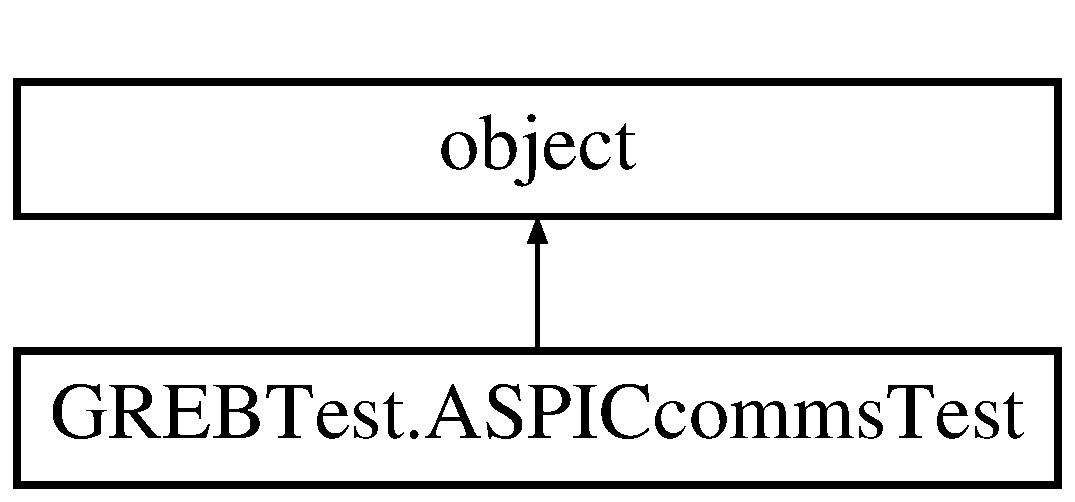
\includegraphics[height=2.000000cm]{class_g_r_e_b_test_1_1_a_s_p_i_ccomms_test}
\end{center}
\end{figure}
\subsection*{Public Member Functions}
\begin{DoxyCompactItemize}
\item 
def \hyperlink{class_g_r_e_b_test_1_1_a_s_p_i_ccomms_test_aeec16202db802631206bf9a138b00bf3}{\+\_\+\+\_\+init\+\_\+\+\_\+} (self)
\begin{DoxyCompactList}\small\item\em Initialize minimum required variables for test list. \end{DoxyCompactList}\item 
def \hyperlink{class_g_r_e_b_test_1_1_a_s_p_i_ccomms_test_aad41625a1dd3747f5adce6fc0b695f1a}{run\+Test} (self)
\begin{DoxyCompactList}\small\item\em Run the test, save output to state variables. \end{DoxyCompactList}\item 
def \hyperlink{class_g_r_e_b_test_1_1_a_s_p_i_ccomms_test_adf8e1bc11cfaeec4f4c38de815260489}{summarize} (self, summary)
\begin{DoxyCompactList}\small\item\em Summarize the test results for the cover page of the report. \end{DoxyCompactList}\item 
def \hyperlink{class_g_r_e_b_test_1_1_a_s_p_i_ccomms_test_a700281a57d921609bc83feaca6f63d81}{report} (self, pdf, report\+Path)
\begin{DoxyCompactList}\small\item\em generate this test\textquotesingle{}s page in the P\+DF report. \end{DoxyCompactList}\end{DoxyCompactItemize}


\subsection{Detailed Description}
Tests that the board can communicate with the A\+S\+P\+I\+CS. 



\subsection{Constructor \& Destructor Documentation}
\index{G\+R\+E\+B\+Test\+::\+A\+S\+P\+I\+Ccomms\+Test@{G\+R\+E\+B\+Test\+::\+A\+S\+P\+I\+Ccomms\+Test}!\+\_\+\+\_\+init\+\_\+\+\_\+@{\+\_\+\+\_\+init\+\_\+\+\_\+}}
\index{\+\_\+\+\_\+init\+\_\+\+\_\+@{\+\_\+\+\_\+init\+\_\+\+\_\+}!G\+R\+E\+B\+Test\+::\+A\+S\+P\+I\+Ccomms\+Test@{G\+R\+E\+B\+Test\+::\+A\+S\+P\+I\+Ccomms\+Test}}
\subsubsection[{\texorpdfstring{\+\_\+\+\_\+init\+\_\+\+\_\+(self)}{__init__(self)}}]{\setlength{\rightskip}{0pt plus 5cm}def G\+R\+E\+B\+Test.\+A\+S\+P\+I\+Ccomms\+Test.\+\_\+\+\_\+init\+\_\+\+\_\+ (
\begin{DoxyParamCaption}
\item[{}]{self}
\end{DoxyParamCaption}
)}\hypertarget{class_g_r_e_b_test_1_1_a_s_p_i_ccomms_test_aeec16202db802631206bf9a138b00bf3}{}\label{class_g_r_e_b_test_1_1_a_s_p_i_ccomms_test_aeec16202db802631206bf9a138b00bf3}


Initialize minimum required variables for test list. 



\subsection{Member Function Documentation}
\index{G\+R\+E\+B\+Test\+::\+A\+S\+P\+I\+Ccomms\+Test@{G\+R\+E\+B\+Test\+::\+A\+S\+P\+I\+Ccomms\+Test}!report@{report}}
\index{report@{report}!G\+R\+E\+B\+Test\+::\+A\+S\+P\+I\+Ccomms\+Test@{G\+R\+E\+B\+Test\+::\+A\+S\+P\+I\+Ccomms\+Test}}
\subsubsection[{\texorpdfstring{report(self, pdf, report\+Path)}{report(self, pdf, reportPath)}}]{\setlength{\rightskip}{0pt plus 5cm}def G\+R\+E\+B\+Test.\+A\+S\+P\+I\+Ccomms\+Test.\+report (
\begin{DoxyParamCaption}
\item[{}]{self, }
\item[{}]{pdf, }
\item[{}]{report\+Path}
\end{DoxyParamCaption}
)}\hypertarget{class_g_r_e_b_test_1_1_a_s_p_i_ccomms_test_a700281a57d921609bc83feaca6f63d81}{}\label{class_g_r_e_b_test_1_1_a_s_p_i_ccomms_test_a700281a57d921609bc83feaca6f63d81}


generate this test\textquotesingle{}s page in the P\+DF report. 


\begin{DoxyParams}{Parameters}
{\em pdf} & pyfpdf-\/compatible P\+DF object. \\
\hline
{\em report\+Path} & Path of directory containing the pdf report \\
\hline
\end{DoxyParams}
\index{G\+R\+E\+B\+Test\+::\+A\+S\+P\+I\+Ccomms\+Test@{G\+R\+E\+B\+Test\+::\+A\+S\+P\+I\+Ccomms\+Test}!run\+Test@{run\+Test}}
\index{run\+Test@{run\+Test}!G\+R\+E\+B\+Test\+::\+A\+S\+P\+I\+Ccomms\+Test@{G\+R\+E\+B\+Test\+::\+A\+S\+P\+I\+Ccomms\+Test}}
\subsubsection[{\texorpdfstring{run\+Test(self)}{runTest(self)}}]{\setlength{\rightskip}{0pt plus 5cm}def G\+R\+E\+B\+Test.\+A\+S\+P\+I\+Ccomms\+Test.\+run\+Test (
\begin{DoxyParamCaption}
\item[{}]{self}
\end{DoxyParamCaption}
)}\hypertarget{class_g_r_e_b_test_1_1_a_s_p_i_ccomms_test_aad41625a1dd3747f5adce6fc0b695f1a}{}\label{class_g_r_e_b_test_1_1_a_s_p_i_ccomms_test_aad41625a1dd3747f5adce6fc0b695f1a}


Run the test, save output to state variables. 

\index{G\+R\+E\+B\+Test\+::\+A\+S\+P\+I\+Ccomms\+Test@{G\+R\+E\+B\+Test\+::\+A\+S\+P\+I\+Ccomms\+Test}!summarize@{summarize}}
\index{summarize@{summarize}!G\+R\+E\+B\+Test\+::\+A\+S\+P\+I\+Ccomms\+Test@{G\+R\+E\+B\+Test\+::\+A\+S\+P\+I\+Ccomms\+Test}}
\subsubsection[{\texorpdfstring{summarize(self, summary)}{summarize(self, summary)}}]{\setlength{\rightskip}{0pt plus 5cm}def G\+R\+E\+B\+Test.\+A\+S\+P\+I\+Ccomms\+Test.\+summarize (
\begin{DoxyParamCaption}
\item[{}]{self, }
\item[{}]{summary}
\end{DoxyParamCaption}
)}\hypertarget{class_g_r_e_b_test_1_1_a_s_p_i_ccomms_test_adf8e1bc11cfaeec4f4c38de815260489}{}\label{class_g_r_e_b_test_1_1_a_s_p_i_ccomms_test_adf8e1bc11cfaeec4f4c38de815260489}


Summarize the test results for the cover page of the report. 


\begin{DoxyParams}{Parameters}
{\em summary} & \hyperlink{class_g_r_e_b_test_1_1_summary}{Summary} obejct passed from Functional\+Test() \\
\hline
\end{DoxyParams}


The documentation for this class was generated from the following file\+:\begin{DoxyCompactItemize}
\item 
\hyperlink{_g_r_e_b_test_8py}{G\+R\+E\+B\+Test.\+py}\end{DoxyCompactItemize}

\hypertarget{class_v_s_t_test_1_1_a_s_p_i_ccomms_test}{}\section{V\+S\+T\+Test.\+A\+S\+P\+I\+Ccomms\+Test Class Reference}
\label{class_v_s_t_test_1_1_a_s_p_i_ccomms_test}\index{V\+S\+T\+Test.\+A\+S\+P\+I\+Ccomms\+Test@{V\+S\+T\+Test.\+A\+S\+P\+I\+Ccomms\+Test}}


Tests that the board can communicate with the A\+S\+P\+I\+CS.  


Inheritance diagram for V\+S\+T\+Test.\+A\+S\+P\+I\+Ccomms\+Test\+:\begin{figure}[H]
\begin{center}
\leavevmode
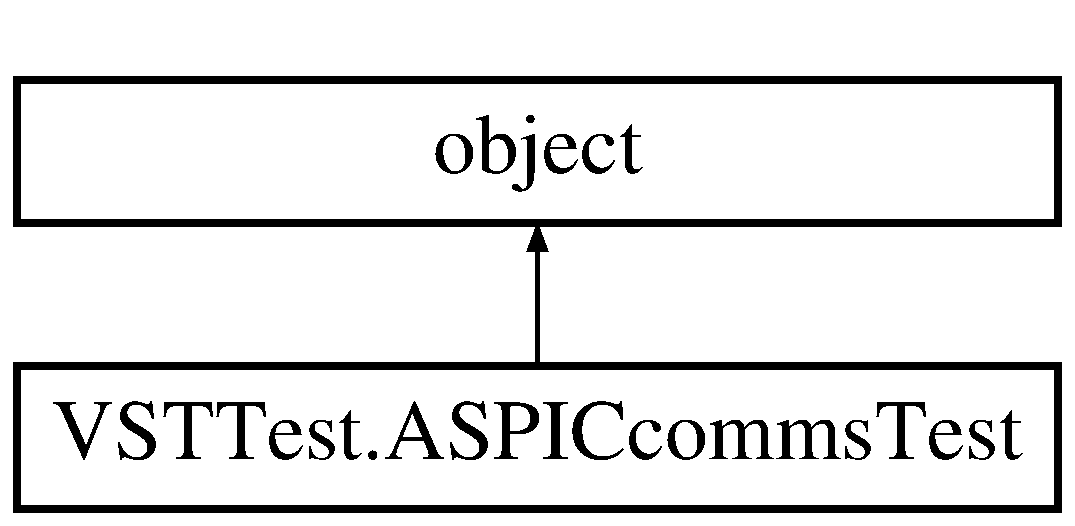
\includegraphics[height=2.000000cm]{class_v_s_t_test_1_1_a_s_p_i_ccomms_test}
\end{center}
\end{figure}
\subsection*{Public Member Functions}
\begin{DoxyCompactItemize}
\item 
def \hyperlink{class_v_s_t_test_1_1_a_s_p_i_ccomms_test_a69362dea820d5e167543f4ea1fb86a08}{\+\_\+\+\_\+init\+\_\+\+\_\+} (self)
\begin{DoxyCompactList}\small\item\em Initialize minimum required variables for test list. \end{DoxyCompactList}\item 
def \hyperlink{class_v_s_t_test_1_1_a_s_p_i_ccomms_test_af7140cb7fcc2a61ab7b0c2c080f78cb8}{run\+Test} (self)
\begin{DoxyCompactList}\small\item\em Run the test, save output to state variables. \end{DoxyCompactList}\item 
def \hyperlink{class_v_s_t_test_1_1_a_s_p_i_ccomms_test_a1c8a9a15b609498fba74d34c1250f8dd}{summarize} (self, summary)
\begin{DoxyCompactList}\small\item\em Summarize the test results for the cover page of the report. \end{DoxyCompactList}\item 
def \hyperlink{class_v_s_t_test_1_1_a_s_p_i_ccomms_test_ab0d44b669fffb02c1a1159ad28f857f8}{report} (self, pdf, report\+Path)
\begin{DoxyCompactList}\small\item\em generate this test\textquotesingle{}s page in the P\+DF report. \end{DoxyCompactList}\end{DoxyCompactItemize}


\subsection{Detailed Description}
Tests that the board can communicate with the A\+S\+P\+I\+CS. 



\subsection{Constructor \& Destructor Documentation}
\index{V\+S\+T\+Test\+::\+A\+S\+P\+I\+Ccomms\+Test@{V\+S\+T\+Test\+::\+A\+S\+P\+I\+Ccomms\+Test}!\+\_\+\+\_\+init\+\_\+\+\_\+@{\+\_\+\+\_\+init\+\_\+\+\_\+}}
\index{\+\_\+\+\_\+init\+\_\+\+\_\+@{\+\_\+\+\_\+init\+\_\+\+\_\+}!V\+S\+T\+Test\+::\+A\+S\+P\+I\+Ccomms\+Test@{V\+S\+T\+Test\+::\+A\+S\+P\+I\+Ccomms\+Test}}
\subsubsection[{\texorpdfstring{\+\_\+\+\_\+init\+\_\+\+\_\+(self)}{__init__(self)}}]{\setlength{\rightskip}{0pt plus 5cm}def V\+S\+T\+Test.\+A\+S\+P\+I\+Ccomms\+Test.\+\_\+\+\_\+init\+\_\+\+\_\+ (
\begin{DoxyParamCaption}
\item[{}]{self}
\end{DoxyParamCaption}
)}\hypertarget{class_v_s_t_test_1_1_a_s_p_i_ccomms_test_a69362dea820d5e167543f4ea1fb86a08}{}\label{class_v_s_t_test_1_1_a_s_p_i_ccomms_test_a69362dea820d5e167543f4ea1fb86a08}


Initialize minimum required variables for test list. 



\subsection{Member Function Documentation}
\index{V\+S\+T\+Test\+::\+A\+S\+P\+I\+Ccomms\+Test@{V\+S\+T\+Test\+::\+A\+S\+P\+I\+Ccomms\+Test}!report@{report}}
\index{report@{report}!V\+S\+T\+Test\+::\+A\+S\+P\+I\+Ccomms\+Test@{V\+S\+T\+Test\+::\+A\+S\+P\+I\+Ccomms\+Test}}
\subsubsection[{\texorpdfstring{report(self, pdf, report\+Path)}{report(self, pdf, reportPath)}}]{\setlength{\rightskip}{0pt plus 5cm}def V\+S\+T\+Test.\+A\+S\+P\+I\+Ccomms\+Test.\+report (
\begin{DoxyParamCaption}
\item[{}]{self, }
\item[{}]{pdf, }
\item[{}]{report\+Path}
\end{DoxyParamCaption}
)}\hypertarget{class_v_s_t_test_1_1_a_s_p_i_ccomms_test_ab0d44b669fffb02c1a1159ad28f857f8}{}\label{class_v_s_t_test_1_1_a_s_p_i_ccomms_test_ab0d44b669fffb02c1a1159ad28f857f8}


generate this test\textquotesingle{}s page in the P\+DF report. 


\begin{DoxyParams}{Parameters}
{\em pdf} & pyfpdf-\/compatible P\+DF object. \\
\hline
{\em report\+Path} & Path of directory containing the pdf report \\
\hline
\end{DoxyParams}
\index{V\+S\+T\+Test\+::\+A\+S\+P\+I\+Ccomms\+Test@{V\+S\+T\+Test\+::\+A\+S\+P\+I\+Ccomms\+Test}!run\+Test@{run\+Test}}
\index{run\+Test@{run\+Test}!V\+S\+T\+Test\+::\+A\+S\+P\+I\+Ccomms\+Test@{V\+S\+T\+Test\+::\+A\+S\+P\+I\+Ccomms\+Test}}
\subsubsection[{\texorpdfstring{run\+Test(self)}{runTest(self)}}]{\setlength{\rightskip}{0pt plus 5cm}def V\+S\+T\+Test.\+A\+S\+P\+I\+Ccomms\+Test.\+run\+Test (
\begin{DoxyParamCaption}
\item[{}]{self}
\end{DoxyParamCaption}
)}\hypertarget{class_v_s_t_test_1_1_a_s_p_i_ccomms_test_af7140cb7fcc2a61ab7b0c2c080f78cb8}{}\label{class_v_s_t_test_1_1_a_s_p_i_ccomms_test_af7140cb7fcc2a61ab7b0c2c080f78cb8}


Run the test, save output to state variables. 

\index{V\+S\+T\+Test\+::\+A\+S\+P\+I\+Ccomms\+Test@{V\+S\+T\+Test\+::\+A\+S\+P\+I\+Ccomms\+Test}!summarize@{summarize}}
\index{summarize@{summarize}!V\+S\+T\+Test\+::\+A\+S\+P\+I\+Ccomms\+Test@{V\+S\+T\+Test\+::\+A\+S\+P\+I\+Ccomms\+Test}}
\subsubsection[{\texorpdfstring{summarize(self, summary)}{summarize(self, summary)}}]{\setlength{\rightskip}{0pt plus 5cm}def V\+S\+T\+Test.\+A\+S\+P\+I\+Ccomms\+Test.\+summarize (
\begin{DoxyParamCaption}
\item[{}]{self, }
\item[{}]{summary}
\end{DoxyParamCaption}
)}\hypertarget{class_v_s_t_test_1_1_a_s_p_i_ccomms_test_a1c8a9a15b609498fba74d34c1250f8dd}{}\label{class_v_s_t_test_1_1_a_s_p_i_ccomms_test_a1c8a9a15b609498fba74d34c1250f8dd}


Summarize the test results for the cover page of the report. 


\begin{DoxyParams}{Parameters}
{\em summary} & \hyperlink{class_v_s_t_test_1_1_summary}{Summary} obejct passed from Functional\+Test() \\
\hline
\end{DoxyParams}


The documentation for this class was generated from the following file\+:\begin{DoxyCompactItemize}
\item 
\hyperlink{_v_s_t_test_8py}{V\+S\+T\+Test.\+py}\end{DoxyCompactItemize}

\hypertarget{class_w_r_e_b_test_1_1_a_s_p_i_ccomms_test}{}\section{W\+R\+E\+B\+Test.\+A\+S\+P\+I\+Ccomms\+Test Class Reference}
\label{class_w_r_e_b_test_1_1_a_s_p_i_ccomms_test}\index{W\+R\+E\+B\+Test.\+A\+S\+P\+I\+Ccomms\+Test@{W\+R\+E\+B\+Test.\+A\+S\+P\+I\+Ccomms\+Test}}


Tests that the board can communicate with the A\+S\+P\+I\+CS.  


Inheritance diagram for W\+R\+E\+B\+Test.\+A\+S\+P\+I\+Ccomms\+Test\+:\begin{figure}[H]
\begin{center}
\leavevmode
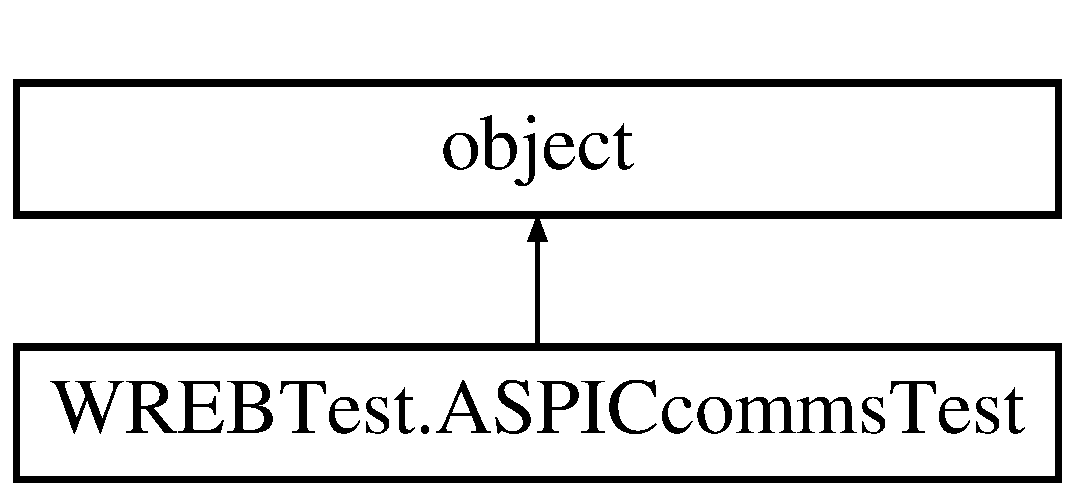
\includegraphics[height=2.000000cm]{class_w_r_e_b_test_1_1_a_s_p_i_ccomms_test}
\end{center}
\end{figure}
\subsection*{Public Member Functions}
\begin{DoxyCompactItemize}
\item 
def \hyperlink{class_w_r_e_b_test_1_1_a_s_p_i_ccomms_test_accfa18c4f22917c2d1ed89b083f02615}{\+\_\+\+\_\+init\+\_\+\+\_\+} (self)
\begin{DoxyCompactList}\small\item\em Initialize minimum required variables for test list. \end{DoxyCompactList}\item 
def \hyperlink{class_w_r_e_b_test_1_1_a_s_p_i_ccomms_test_ab1d5e43e09a6ba9656a27631614cd268}{run\+Test} (self)
\begin{DoxyCompactList}\small\item\em Run the test, save output to state variables. \end{DoxyCompactList}\item 
def \hyperlink{class_w_r_e_b_test_1_1_a_s_p_i_ccomms_test_a359865f04f303787eb68e5f29409a768}{summarize} (self, summary)
\begin{DoxyCompactList}\small\item\em Summarize the test results for the cover page of the report. \end{DoxyCompactList}\item 
def \hyperlink{class_w_r_e_b_test_1_1_a_s_p_i_ccomms_test_a22d5544b8f7c5d9373b9804bb716cc40}{report} (self, pdf, report\+Path)
\begin{DoxyCompactList}\small\item\em generate this test\textquotesingle{}s page in the P\+DF report. \end{DoxyCompactList}\end{DoxyCompactItemize}


\subsection{Detailed Description}
Tests that the board can communicate with the A\+S\+P\+I\+CS. 



\subsection{Constructor \& Destructor Documentation}
\index{W\+R\+E\+B\+Test\+::\+A\+S\+P\+I\+Ccomms\+Test@{W\+R\+E\+B\+Test\+::\+A\+S\+P\+I\+Ccomms\+Test}!\+\_\+\+\_\+init\+\_\+\+\_\+@{\+\_\+\+\_\+init\+\_\+\+\_\+}}
\index{\+\_\+\+\_\+init\+\_\+\+\_\+@{\+\_\+\+\_\+init\+\_\+\+\_\+}!W\+R\+E\+B\+Test\+::\+A\+S\+P\+I\+Ccomms\+Test@{W\+R\+E\+B\+Test\+::\+A\+S\+P\+I\+Ccomms\+Test}}
\subsubsection[{\texorpdfstring{\+\_\+\+\_\+init\+\_\+\+\_\+(self)}{__init__(self)}}]{\setlength{\rightskip}{0pt plus 5cm}def W\+R\+E\+B\+Test.\+A\+S\+P\+I\+Ccomms\+Test.\+\_\+\+\_\+init\+\_\+\+\_\+ (
\begin{DoxyParamCaption}
\item[{}]{self}
\end{DoxyParamCaption}
)}\hypertarget{class_w_r_e_b_test_1_1_a_s_p_i_ccomms_test_accfa18c4f22917c2d1ed89b083f02615}{}\label{class_w_r_e_b_test_1_1_a_s_p_i_ccomms_test_accfa18c4f22917c2d1ed89b083f02615}


Initialize minimum required variables for test list. 



\subsection{Member Function Documentation}
\index{W\+R\+E\+B\+Test\+::\+A\+S\+P\+I\+Ccomms\+Test@{W\+R\+E\+B\+Test\+::\+A\+S\+P\+I\+Ccomms\+Test}!report@{report}}
\index{report@{report}!W\+R\+E\+B\+Test\+::\+A\+S\+P\+I\+Ccomms\+Test@{W\+R\+E\+B\+Test\+::\+A\+S\+P\+I\+Ccomms\+Test}}
\subsubsection[{\texorpdfstring{report(self, pdf, report\+Path)}{report(self, pdf, reportPath)}}]{\setlength{\rightskip}{0pt plus 5cm}def W\+R\+E\+B\+Test.\+A\+S\+P\+I\+Ccomms\+Test.\+report (
\begin{DoxyParamCaption}
\item[{}]{self, }
\item[{}]{pdf, }
\item[{}]{report\+Path}
\end{DoxyParamCaption}
)}\hypertarget{class_w_r_e_b_test_1_1_a_s_p_i_ccomms_test_a22d5544b8f7c5d9373b9804bb716cc40}{}\label{class_w_r_e_b_test_1_1_a_s_p_i_ccomms_test_a22d5544b8f7c5d9373b9804bb716cc40}


generate this test\textquotesingle{}s page in the P\+DF report. 


\begin{DoxyParams}{Parameters}
{\em pdf} & pyfpdf-\/compatible P\+DF object. \\
\hline
{\em report\+Path} & Path of directory containing the pdf report \\
\hline
\end{DoxyParams}
\index{W\+R\+E\+B\+Test\+::\+A\+S\+P\+I\+Ccomms\+Test@{W\+R\+E\+B\+Test\+::\+A\+S\+P\+I\+Ccomms\+Test}!run\+Test@{run\+Test}}
\index{run\+Test@{run\+Test}!W\+R\+E\+B\+Test\+::\+A\+S\+P\+I\+Ccomms\+Test@{W\+R\+E\+B\+Test\+::\+A\+S\+P\+I\+Ccomms\+Test}}
\subsubsection[{\texorpdfstring{run\+Test(self)}{runTest(self)}}]{\setlength{\rightskip}{0pt plus 5cm}def W\+R\+E\+B\+Test.\+A\+S\+P\+I\+Ccomms\+Test.\+run\+Test (
\begin{DoxyParamCaption}
\item[{}]{self}
\end{DoxyParamCaption}
)}\hypertarget{class_w_r_e_b_test_1_1_a_s_p_i_ccomms_test_ab1d5e43e09a6ba9656a27631614cd268}{}\label{class_w_r_e_b_test_1_1_a_s_p_i_ccomms_test_ab1d5e43e09a6ba9656a27631614cd268}


Run the test, save output to state variables. 

\index{W\+R\+E\+B\+Test\+::\+A\+S\+P\+I\+Ccomms\+Test@{W\+R\+E\+B\+Test\+::\+A\+S\+P\+I\+Ccomms\+Test}!summarize@{summarize}}
\index{summarize@{summarize}!W\+R\+E\+B\+Test\+::\+A\+S\+P\+I\+Ccomms\+Test@{W\+R\+E\+B\+Test\+::\+A\+S\+P\+I\+Ccomms\+Test}}
\subsubsection[{\texorpdfstring{summarize(self, summary)}{summarize(self, summary)}}]{\setlength{\rightskip}{0pt plus 5cm}def W\+R\+E\+B\+Test.\+A\+S\+P\+I\+Ccomms\+Test.\+summarize (
\begin{DoxyParamCaption}
\item[{}]{self, }
\item[{}]{summary}
\end{DoxyParamCaption}
)}\hypertarget{class_w_r_e_b_test_1_1_a_s_p_i_ccomms_test_a359865f04f303787eb68e5f29409a768}{}\label{class_w_r_e_b_test_1_1_a_s_p_i_ccomms_test_a359865f04f303787eb68e5f29409a768}


Summarize the test results for the cover page of the report. 


\begin{DoxyParams}{Parameters}
{\em summary} & \hyperlink{class_w_r_e_b_test_1_1_summary}{Summary} obejct passed from Functional\+Test() \\
\hline
\end{DoxyParams}


The documentation for this class was generated from the following file\+:\begin{DoxyCompactItemize}
\item 
\hyperlink{_w_r_e_b_test_8py}{W\+R\+E\+B\+Test.\+py}\end{DoxyCompactItemize}

\hypertarget{class_g_r_e_b_test_1_1_a_s_p_i_c_logging}{}\section{G\+R\+E\+B\+Test.\+A\+S\+P\+I\+C\+Logging Class Reference}
\label{class_g_r_e_b_test_1_1_a_s_p_i_c_logging}\index{G\+R\+E\+B\+Test.\+A\+S\+P\+I\+C\+Logging@{G\+R\+E\+B\+Test.\+A\+S\+P\+I\+C\+Logging}}


Continuously measure noise distribution in A\+S\+P\+I\+Cs.  


Inheritance diagram for G\+R\+E\+B\+Test.\+A\+S\+P\+I\+C\+Logging\+:\begin{figure}[H]
\begin{center}
\leavevmode
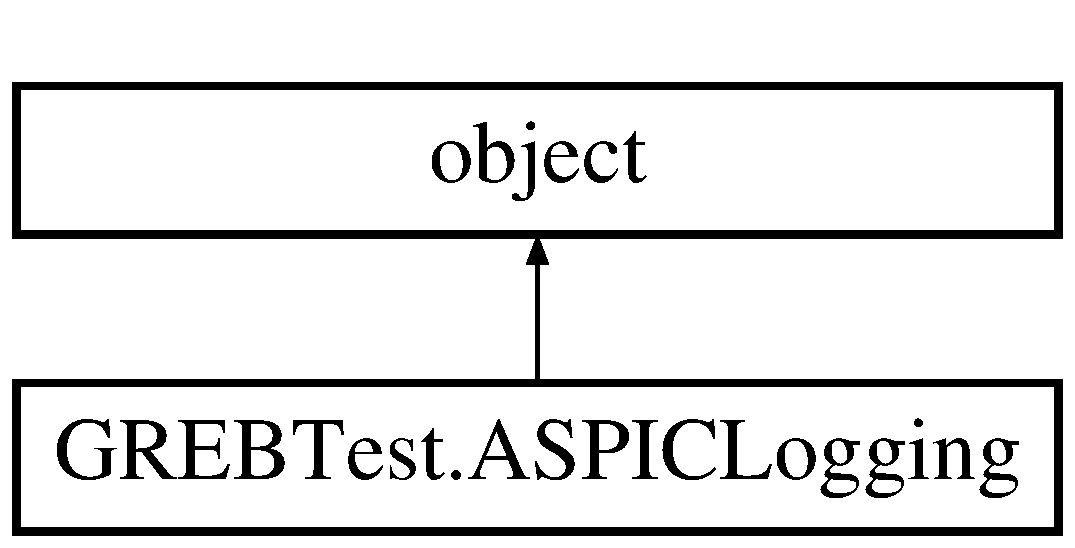
\includegraphics[height=2.000000cm]{class_g_r_e_b_test_1_1_a_s_p_i_c_logging}
\end{center}
\end{figure}
\subsection*{Public Member Functions}
\begin{DoxyCompactItemize}
\item 
def \hyperlink{class_g_r_e_b_test_1_1_a_s_p_i_c_logging_a009d36147be8ad7628f5c7cd099759a7}{\+\_\+\+\_\+init\+\_\+\+\_\+} (self, values\+To\+Read=None)
\begin{DoxyCompactList}\small\item\em Initialize minimum required variables for test list. \end{DoxyCompactList}\item 
def \hyperlink{class_g_r_e_b_test_1_1_a_s_p_i_c_logging_a649325e8307acc4e94aa21d5c5b3d311}{run\+Test} (self, delay=5 $\ast$60)
\begin{DoxyCompactList}\small\item\em Continuously log A\+S\+P\+IC images every time interval. \end{DoxyCompactList}\item 
def \hyperlink{class_g_r_e_b_test_1_1_a_s_p_i_c_logging_a86d905193d1549a3b86f4bca8e94fc4d}{summarize} (self, summary)
\begin{DoxyCompactList}\small\item\em Summarize the test results for the cover page of the report. \end{DoxyCompactList}\item 
def \hyperlink{class_g_r_e_b_test_1_1_a_s_p_i_c_logging_a4d12b049f243febdec8b378cda8ae885}{report} (self, pdf)
\begin{DoxyCompactList}\small\item\em generate this test\textquotesingle{}s page in the P\+DF report. \end{DoxyCompactList}\end{DoxyCompactItemize}


\subsection{Detailed Description}
Continuously measure noise distribution in A\+S\+P\+I\+Cs. 

Must be run with -\/l enabled. 

\subsection{Constructor \& Destructor Documentation}
\index{G\+R\+E\+B\+Test\+::\+A\+S\+P\+I\+C\+Logging@{G\+R\+E\+B\+Test\+::\+A\+S\+P\+I\+C\+Logging}!\+\_\+\+\_\+init\+\_\+\+\_\+@{\+\_\+\+\_\+init\+\_\+\+\_\+}}
\index{\+\_\+\+\_\+init\+\_\+\+\_\+@{\+\_\+\+\_\+init\+\_\+\+\_\+}!G\+R\+E\+B\+Test\+::\+A\+S\+P\+I\+C\+Logging@{G\+R\+E\+B\+Test\+::\+A\+S\+P\+I\+C\+Logging}}
\subsubsection[{\texorpdfstring{\+\_\+\+\_\+init\+\_\+\+\_\+(self, values\+To\+Read=\+None)}{__init__(self, valuesToRead=None)}}]{\setlength{\rightskip}{0pt plus 5cm}def G\+R\+E\+B\+Test.\+A\+S\+P\+I\+C\+Logging.\+\_\+\+\_\+init\+\_\+\+\_\+ (
\begin{DoxyParamCaption}
\item[{}]{self, }
\item[{}]{values\+To\+Read = {\ttfamily None}}
\end{DoxyParamCaption}
)}\hypertarget{class_g_r_e_b_test_1_1_a_s_p_i_c_logging_a009d36147be8ad7628f5c7cd099759a7}{}\label{class_g_r_e_b_test_1_1_a_s_p_i_c_logging_a009d36147be8ad7628f5c7cd099759a7}


Initialize minimum required variables for test list. 



\subsection{Member Function Documentation}
\index{G\+R\+E\+B\+Test\+::\+A\+S\+P\+I\+C\+Logging@{G\+R\+E\+B\+Test\+::\+A\+S\+P\+I\+C\+Logging}!report@{report}}
\index{report@{report}!G\+R\+E\+B\+Test\+::\+A\+S\+P\+I\+C\+Logging@{G\+R\+E\+B\+Test\+::\+A\+S\+P\+I\+C\+Logging}}
\subsubsection[{\texorpdfstring{report(self, pdf)}{report(self, pdf)}}]{\setlength{\rightskip}{0pt plus 5cm}def G\+R\+E\+B\+Test.\+A\+S\+P\+I\+C\+Logging.\+report (
\begin{DoxyParamCaption}
\item[{}]{self, }
\item[{}]{pdf}
\end{DoxyParamCaption}
)}\hypertarget{class_g_r_e_b_test_1_1_a_s_p_i_c_logging_a4d12b049f243febdec8b378cda8ae885}{}\label{class_g_r_e_b_test_1_1_a_s_p_i_c_logging_a4d12b049f243febdec8b378cda8ae885}


generate this test\textquotesingle{}s page in the P\+DF report. 


\begin{DoxyParams}{Parameters}
{\em pdf} & pyfpdf-\/compatible P\+DF object. \\
\hline
\end{DoxyParams}
\index{G\+R\+E\+B\+Test\+::\+A\+S\+P\+I\+C\+Logging@{G\+R\+E\+B\+Test\+::\+A\+S\+P\+I\+C\+Logging}!run\+Test@{run\+Test}}
\index{run\+Test@{run\+Test}!G\+R\+E\+B\+Test\+::\+A\+S\+P\+I\+C\+Logging@{G\+R\+E\+B\+Test\+::\+A\+S\+P\+I\+C\+Logging}}
\subsubsection[{\texorpdfstring{run\+Test(self, delay=5 $\ast$60)}{runTest(self, delay=5 *60)}}]{\setlength{\rightskip}{0pt plus 5cm}def G\+R\+E\+B\+Test.\+A\+S\+P\+I\+C\+Logging.\+run\+Test (
\begin{DoxyParamCaption}
\item[{}]{self, }
\item[{}]{delay = {\ttfamily 5~$\ast$~60}}
\end{DoxyParamCaption}
)}\hypertarget{class_g_r_e_b_test_1_1_a_s_p_i_c_logging_a649325e8307acc4e94aa21d5c5b3d311}{}\label{class_g_r_e_b_test_1_1_a_s_p_i_c_logging_a649325e8307acc4e94aa21d5c5b3d311}


Continuously log A\+S\+P\+IC images every time interval. 

\index{G\+R\+E\+B\+Test\+::\+A\+S\+P\+I\+C\+Logging@{G\+R\+E\+B\+Test\+::\+A\+S\+P\+I\+C\+Logging}!summarize@{summarize}}
\index{summarize@{summarize}!G\+R\+E\+B\+Test\+::\+A\+S\+P\+I\+C\+Logging@{G\+R\+E\+B\+Test\+::\+A\+S\+P\+I\+C\+Logging}}
\subsubsection[{\texorpdfstring{summarize(self, summary)}{summarize(self, summary)}}]{\setlength{\rightskip}{0pt plus 5cm}def G\+R\+E\+B\+Test.\+A\+S\+P\+I\+C\+Logging.\+summarize (
\begin{DoxyParamCaption}
\item[{}]{self, }
\item[{}]{summary}
\end{DoxyParamCaption}
)}\hypertarget{class_g_r_e_b_test_1_1_a_s_p_i_c_logging_a86d905193d1549a3b86f4bca8e94fc4d}{}\label{class_g_r_e_b_test_1_1_a_s_p_i_c_logging_a86d905193d1549a3b86f4bca8e94fc4d}


Summarize the test results for the cover page of the report. 


\begin{DoxyParams}{Parameters}
{\em summary} & \hyperlink{class_g_r_e_b_test_1_1_summary}{Summary} obejct passed from Functional\+Test() \\
\hline
\end{DoxyParams}


The documentation for this class was generated from the following file\+:\begin{DoxyCompactItemize}
\item 
\hyperlink{_g_r_e_b_test_8py}{G\+R\+E\+B\+Test.\+py}\end{DoxyCompactItemize}

\hypertarget{class_v_s_t_test_1_1_a_s_p_i_c_logging}{}\section{V\+S\+T\+Test.\+A\+S\+P\+I\+C\+Logging Class Reference}
\label{class_v_s_t_test_1_1_a_s_p_i_c_logging}\index{V\+S\+T\+Test.\+A\+S\+P\+I\+C\+Logging@{V\+S\+T\+Test.\+A\+S\+P\+I\+C\+Logging}}


Continuously measure noise distribution in A\+S\+P\+I\+Cs.  


Inheritance diagram for V\+S\+T\+Test.\+A\+S\+P\+I\+C\+Logging\+:\begin{figure}[H]
\begin{center}
\leavevmode
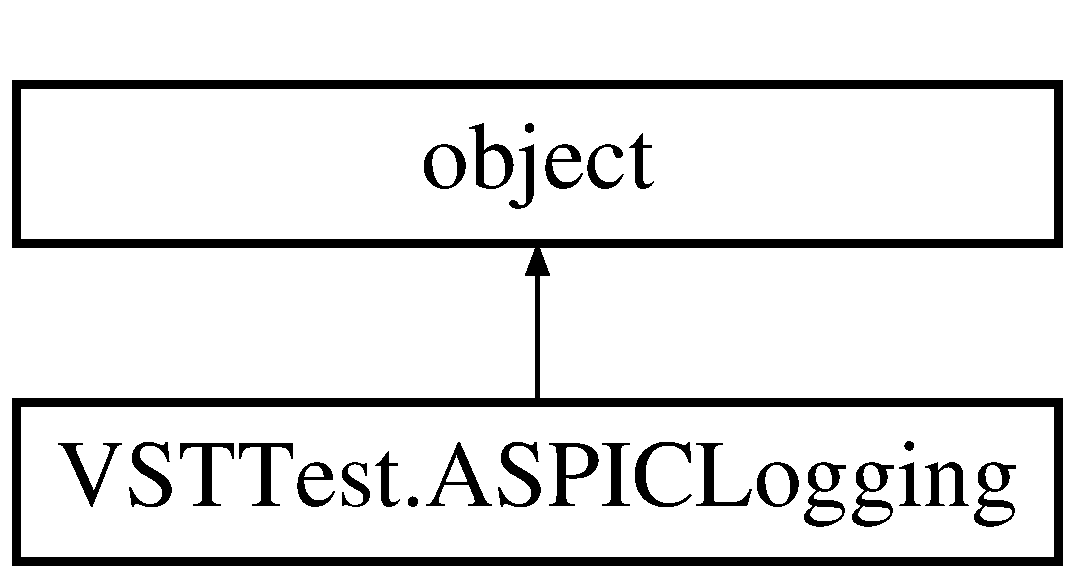
\includegraphics[height=2.000000cm]{class_v_s_t_test_1_1_a_s_p_i_c_logging}
\end{center}
\end{figure}
\subsection*{Public Member Functions}
\begin{DoxyCompactItemize}
\item 
def \hyperlink{class_v_s_t_test_1_1_a_s_p_i_c_logging_a4109e19584640be34d9f2249e210bab5}{\+\_\+\+\_\+init\+\_\+\+\_\+} (self, values\+To\+Read=None)
\begin{DoxyCompactList}\small\item\em Initialize minimum required variables for test list. \end{DoxyCompactList}\item 
def \hyperlink{class_v_s_t_test_1_1_a_s_p_i_c_logging_a9917bfa04e1d09b94eb9baaf2ab192ae}{run\+Test} (self, delay=5 $\ast$60)
\begin{DoxyCompactList}\small\item\em Continuously log A\+S\+P\+IC images every time interval. \end{DoxyCompactList}\item 
def \hyperlink{class_v_s_t_test_1_1_a_s_p_i_c_logging_abc0c3f33d4f4e75da2ddfc529b74bf22}{summarize} (self, summary)
\begin{DoxyCompactList}\small\item\em Summarize the test results for the cover page of the report. \end{DoxyCompactList}\item 
def \hyperlink{class_v_s_t_test_1_1_a_s_p_i_c_logging_ad41e35efcd3ec00652c6ea4774101331}{report} (self, pdf)
\begin{DoxyCompactList}\small\item\em generate this test\textquotesingle{}s page in the P\+DF report. \end{DoxyCompactList}\end{DoxyCompactItemize}


\subsection{Detailed Description}
Continuously measure noise distribution in A\+S\+P\+I\+Cs. 

Must be run with -\/l enabled. 

\subsection{Constructor \& Destructor Documentation}
\index{V\+S\+T\+Test\+::\+A\+S\+P\+I\+C\+Logging@{V\+S\+T\+Test\+::\+A\+S\+P\+I\+C\+Logging}!\+\_\+\+\_\+init\+\_\+\+\_\+@{\+\_\+\+\_\+init\+\_\+\+\_\+}}
\index{\+\_\+\+\_\+init\+\_\+\+\_\+@{\+\_\+\+\_\+init\+\_\+\+\_\+}!V\+S\+T\+Test\+::\+A\+S\+P\+I\+C\+Logging@{V\+S\+T\+Test\+::\+A\+S\+P\+I\+C\+Logging}}
\subsubsection[{\texorpdfstring{\+\_\+\+\_\+init\+\_\+\+\_\+(self, values\+To\+Read=\+None)}{__init__(self, valuesToRead=None)}}]{\setlength{\rightskip}{0pt plus 5cm}def V\+S\+T\+Test.\+A\+S\+P\+I\+C\+Logging.\+\_\+\+\_\+init\+\_\+\+\_\+ (
\begin{DoxyParamCaption}
\item[{}]{self, }
\item[{}]{values\+To\+Read = {\ttfamily None}}
\end{DoxyParamCaption}
)}\hypertarget{class_v_s_t_test_1_1_a_s_p_i_c_logging_a4109e19584640be34d9f2249e210bab5}{}\label{class_v_s_t_test_1_1_a_s_p_i_c_logging_a4109e19584640be34d9f2249e210bab5}


Initialize minimum required variables for test list. 



\subsection{Member Function Documentation}
\index{V\+S\+T\+Test\+::\+A\+S\+P\+I\+C\+Logging@{V\+S\+T\+Test\+::\+A\+S\+P\+I\+C\+Logging}!report@{report}}
\index{report@{report}!V\+S\+T\+Test\+::\+A\+S\+P\+I\+C\+Logging@{V\+S\+T\+Test\+::\+A\+S\+P\+I\+C\+Logging}}
\subsubsection[{\texorpdfstring{report(self, pdf)}{report(self, pdf)}}]{\setlength{\rightskip}{0pt plus 5cm}def V\+S\+T\+Test.\+A\+S\+P\+I\+C\+Logging.\+report (
\begin{DoxyParamCaption}
\item[{}]{self, }
\item[{}]{pdf}
\end{DoxyParamCaption}
)}\hypertarget{class_v_s_t_test_1_1_a_s_p_i_c_logging_ad41e35efcd3ec00652c6ea4774101331}{}\label{class_v_s_t_test_1_1_a_s_p_i_c_logging_ad41e35efcd3ec00652c6ea4774101331}


generate this test\textquotesingle{}s page in the P\+DF report. 


\begin{DoxyParams}{Parameters}
{\em pdf} & pyfpdf-\/compatible P\+DF object. \\
\hline
\end{DoxyParams}
\index{V\+S\+T\+Test\+::\+A\+S\+P\+I\+C\+Logging@{V\+S\+T\+Test\+::\+A\+S\+P\+I\+C\+Logging}!run\+Test@{run\+Test}}
\index{run\+Test@{run\+Test}!V\+S\+T\+Test\+::\+A\+S\+P\+I\+C\+Logging@{V\+S\+T\+Test\+::\+A\+S\+P\+I\+C\+Logging}}
\subsubsection[{\texorpdfstring{run\+Test(self, delay=5 $\ast$60)}{runTest(self, delay=5 *60)}}]{\setlength{\rightskip}{0pt plus 5cm}def V\+S\+T\+Test.\+A\+S\+P\+I\+C\+Logging.\+run\+Test (
\begin{DoxyParamCaption}
\item[{}]{self, }
\item[{}]{delay = {\ttfamily 5~$\ast$~60}}
\end{DoxyParamCaption}
)}\hypertarget{class_v_s_t_test_1_1_a_s_p_i_c_logging_a9917bfa04e1d09b94eb9baaf2ab192ae}{}\label{class_v_s_t_test_1_1_a_s_p_i_c_logging_a9917bfa04e1d09b94eb9baaf2ab192ae}


Continuously log A\+S\+P\+IC images every time interval. 

\index{V\+S\+T\+Test\+::\+A\+S\+P\+I\+C\+Logging@{V\+S\+T\+Test\+::\+A\+S\+P\+I\+C\+Logging}!summarize@{summarize}}
\index{summarize@{summarize}!V\+S\+T\+Test\+::\+A\+S\+P\+I\+C\+Logging@{V\+S\+T\+Test\+::\+A\+S\+P\+I\+C\+Logging}}
\subsubsection[{\texorpdfstring{summarize(self, summary)}{summarize(self, summary)}}]{\setlength{\rightskip}{0pt plus 5cm}def V\+S\+T\+Test.\+A\+S\+P\+I\+C\+Logging.\+summarize (
\begin{DoxyParamCaption}
\item[{}]{self, }
\item[{}]{summary}
\end{DoxyParamCaption}
)}\hypertarget{class_v_s_t_test_1_1_a_s_p_i_c_logging_abc0c3f33d4f4e75da2ddfc529b74bf22}{}\label{class_v_s_t_test_1_1_a_s_p_i_c_logging_abc0c3f33d4f4e75da2ddfc529b74bf22}


Summarize the test results for the cover page of the report. 


\begin{DoxyParams}{Parameters}
{\em summary} & \hyperlink{class_v_s_t_test_1_1_summary}{Summary} obejct passed from Functional\+Test() \\
\hline
\end{DoxyParams}


The documentation for this class was generated from the following file\+:\begin{DoxyCompactItemize}
\item 
\hyperlink{_v_s_t_test_8py}{V\+S\+T\+Test.\+py}\end{DoxyCompactItemize}

\hypertarget{class_w_r_e_b_test_1_1_a_s_p_i_c_logging}{}\section{W\+R\+E\+B\+Test.\+A\+S\+P\+I\+C\+Logging Class Reference}
\label{class_w_r_e_b_test_1_1_a_s_p_i_c_logging}\index{W\+R\+E\+B\+Test.\+A\+S\+P\+I\+C\+Logging@{W\+R\+E\+B\+Test.\+A\+S\+P\+I\+C\+Logging}}


Continuously measure noise distribution in A\+S\+P\+I\+Cs.  


Inheritance diagram for W\+R\+E\+B\+Test.\+A\+S\+P\+I\+C\+Logging\+:\begin{figure}[H]
\begin{center}
\leavevmode
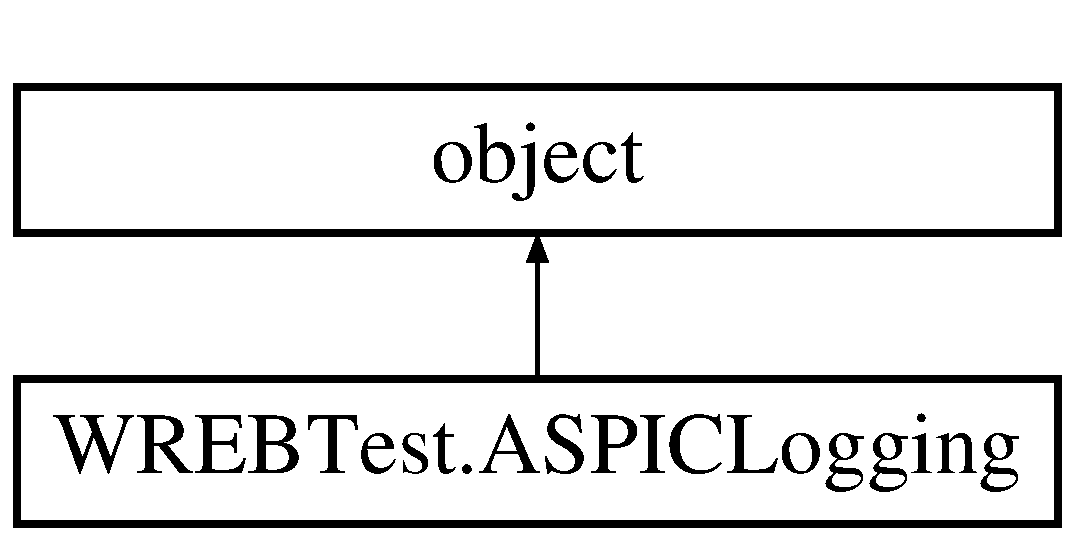
\includegraphics[height=2.000000cm]{class_w_r_e_b_test_1_1_a_s_p_i_c_logging}
\end{center}
\end{figure}
\subsection*{Public Member Functions}
\begin{DoxyCompactItemize}
\item 
def \hyperlink{class_w_r_e_b_test_1_1_a_s_p_i_c_logging_aa57be40a690bbce4458df52fbd61cac3}{\+\_\+\+\_\+init\+\_\+\+\_\+} (self)
\begin{DoxyCompactList}\small\item\em Initialize minimum required variables for test list. \end{DoxyCompactList}\item 
def \hyperlink{class_w_r_e_b_test_1_1_a_s_p_i_c_logging_ab6382a12a1bc12f9865f0a1d8d49acff}{run\+Test} (self, delay=50 $\ast$60)
\begin{DoxyCompactList}\small\item\em Continuously log A\+S\+P\+IC images every time interval. \end{DoxyCompactList}\item 
def \hyperlink{class_w_r_e_b_test_1_1_a_s_p_i_c_logging_a4189d090fcfd601127caa7c59edeb3a1}{summarize} (self, summary)
\begin{DoxyCompactList}\small\item\em Summarize the test results for the cover page of the report. \end{DoxyCompactList}\item 
def \hyperlink{class_w_r_e_b_test_1_1_a_s_p_i_c_logging_a0913af7afc258f537e6a7dc6c5b42bdb}{report} (self, pdf)
\begin{DoxyCompactList}\small\item\em generate this test\textquotesingle{}s page in the P\+DF report. \end{DoxyCompactList}\end{DoxyCompactItemize}


\subsection{Detailed Description}
Continuously measure noise distribution in A\+S\+P\+I\+Cs. 

Must be run with -\/l enabled. 

\subsection{Constructor \& Destructor Documentation}
\index{W\+R\+E\+B\+Test\+::\+A\+S\+P\+I\+C\+Logging@{W\+R\+E\+B\+Test\+::\+A\+S\+P\+I\+C\+Logging}!\+\_\+\+\_\+init\+\_\+\+\_\+@{\+\_\+\+\_\+init\+\_\+\+\_\+}}
\index{\+\_\+\+\_\+init\+\_\+\+\_\+@{\+\_\+\+\_\+init\+\_\+\+\_\+}!W\+R\+E\+B\+Test\+::\+A\+S\+P\+I\+C\+Logging@{W\+R\+E\+B\+Test\+::\+A\+S\+P\+I\+C\+Logging}}
\subsubsection[{\texorpdfstring{\+\_\+\+\_\+init\+\_\+\+\_\+(self)}{__init__(self)}}]{\setlength{\rightskip}{0pt plus 5cm}def W\+R\+E\+B\+Test.\+A\+S\+P\+I\+C\+Logging.\+\_\+\+\_\+init\+\_\+\+\_\+ (
\begin{DoxyParamCaption}
\item[{}]{self}
\end{DoxyParamCaption}
)}\hypertarget{class_w_r_e_b_test_1_1_a_s_p_i_c_logging_aa57be40a690bbce4458df52fbd61cac3}{}\label{class_w_r_e_b_test_1_1_a_s_p_i_c_logging_aa57be40a690bbce4458df52fbd61cac3}


Initialize minimum required variables for test list. 



\subsection{Member Function Documentation}
\index{W\+R\+E\+B\+Test\+::\+A\+S\+P\+I\+C\+Logging@{W\+R\+E\+B\+Test\+::\+A\+S\+P\+I\+C\+Logging}!report@{report}}
\index{report@{report}!W\+R\+E\+B\+Test\+::\+A\+S\+P\+I\+C\+Logging@{W\+R\+E\+B\+Test\+::\+A\+S\+P\+I\+C\+Logging}}
\subsubsection[{\texorpdfstring{report(self, pdf)}{report(self, pdf)}}]{\setlength{\rightskip}{0pt plus 5cm}def W\+R\+E\+B\+Test.\+A\+S\+P\+I\+C\+Logging.\+report (
\begin{DoxyParamCaption}
\item[{}]{self, }
\item[{}]{pdf}
\end{DoxyParamCaption}
)}\hypertarget{class_w_r_e_b_test_1_1_a_s_p_i_c_logging_a0913af7afc258f537e6a7dc6c5b42bdb}{}\label{class_w_r_e_b_test_1_1_a_s_p_i_c_logging_a0913af7afc258f537e6a7dc6c5b42bdb}


generate this test\textquotesingle{}s page in the P\+DF report. 


\begin{DoxyParams}{Parameters}
{\em pdf} & pyfpdf-\/compatible P\+DF object. \\
\hline
\end{DoxyParams}
\index{W\+R\+E\+B\+Test\+::\+A\+S\+P\+I\+C\+Logging@{W\+R\+E\+B\+Test\+::\+A\+S\+P\+I\+C\+Logging}!run\+Test@{run\+Test}}
\index{run\+Test@{run\+Test}!W\+R\+E\+B\+Test\+::\+A\+S\+P\+I\+C\+Logging@{W\+R\+E\+B\+Test\+::\+A\+S\+P\+I\+C\+Logging}}
\subsubsection[{\texorpdfstring{run\+Test(self, delay=50 $\ast$60)}{runTest(self, delay=50 *60)}}]{\setlength{\rightskip}{0pt plus 5cm}def W\+R\+E\+B\+Test.\+A\+S\+P\+I\+C\+Logging.\+run\+Test (
\begin{DoxyParamCaption}
\item[{}]{self, }
\item[{}]{delay = {\ttfamily 50~$\ast$~60}}
\end{DoxyParamCaption}
)}\hypertarget{class_w_r_e_b_test_1_1_a_s_p_i_c_logging_ab6382a12a1bc12f9865f0a1d8d49acff}{}\label{class_w_r_e_b_test_1_1_a_s_p_i_c_logging_ab6382a12a1bc12f9865f0a1d8d49acff}


Continuously log A\+S\+P\+IC images every time interval. 

\index{W\+R\+E\+B\+Test\+::\+A\+S\+P\+I\+C\+Logging@{W\+R\+E\+B\+Test\+::\+A\+S\+P\+I\+C\+Logging}!summarize@{summarize}}
\index{summarize@{summarize}!W\+R\+E\+B\+Test\+::\+A\+S\+P\+I\+C\+Logging@{W\+R\+E\+B\+Test\+::\+A\+S\+P\+I\+C\+Logging}}
\subsubsection[{\texorpdfstring{summarize(self, summary)}{summarize(self, summary)}}]{\setlength{\rightskip}{0pt plus 5cm}def W\+R\+E\+B\+Test.\+A\+S\+P\+I\+C\+Logging.\+summarize (
\begin{DoxyParamCaption}
\item[{}]{self, }
\item[{}]{summary}
\end{DoxyParamCaption}
)}\hypertarget{class_w_r_e_b_test_1_1_a_s_p_i_c_logging_a4189d090fcfd601127caa7c59edeb3a1}{}\label{class_w_r_e_b_test_1_1_a_s_p_i_c_logging_a4189d090fcfd601127caa7c59edeb3a1}


Summarize the test results for the cover page of the report. 


\begin{DoxyParams}{Parameters}
{\em summary} & \hyperlink{class_w_r_e_b_test_1_1_summary}{Summary} obejct passed from Functional\+Test() \\
\hline
\end{DoxyParams}


The documentation for this class was generated from the following file\+:\begin{DoxyCompactItemize}
\item 
\hyperlink{_w_r_e_b_test_8py}{W\+R\+E\+B\+Test.\+py}\end{DoxyCompactItemize}

\hypertarget{class_g_r_e_b_test_1_1_a_s_p_i_c_noise}{}\section{G\+R\+E\+B\+Test.\+A\+S\+P\+I\+C\+Noise Class Reference}
\label{class_g_r_e_b_test_1_1_a_s_p_i_c_noise}\index{G\+R\+E\+B\+Test.\+A\+S\+P\+I\+C\+Noise@{G\+R\+E\+B\+Test.\+A\+S\+P\+I\+C\+Noise}}


Measure noise distribution in A\+S\+P\+I\+Cs for the unclamped, clamped, and reset cases.  


Inheritance diagram for G\+R\+E\+B\+Test.\+A\+S\+P\+I\+C\+Noise\+:\begin{figure}[H]
\begin{center}
\leavevmode
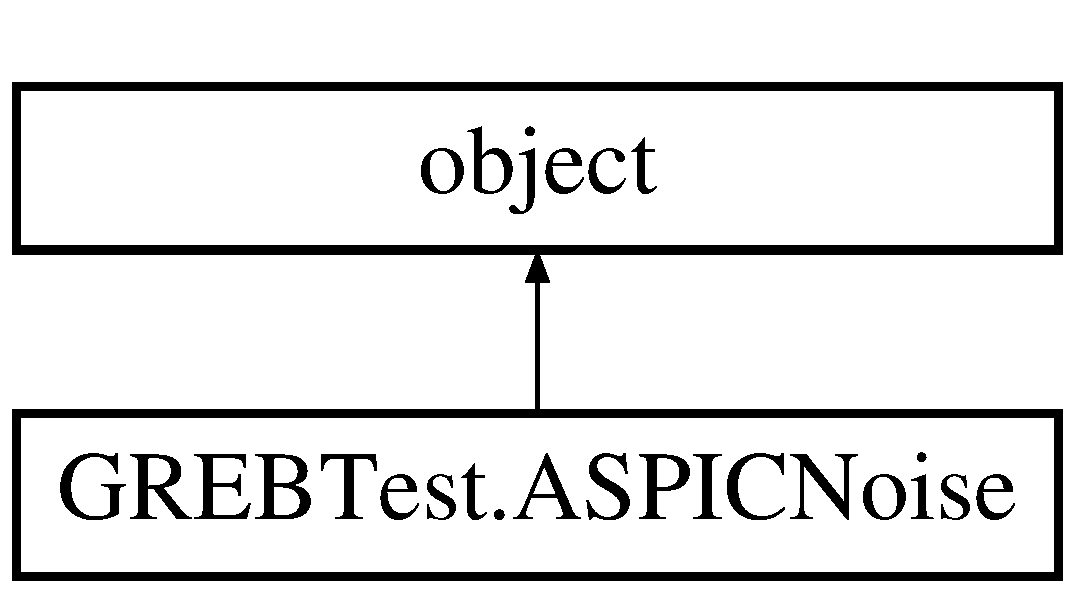
\includegraphics[height=2.000000cm]{class_g_r_e_b_test_1_1_a_s_p_i_c_noise}
\end{center}
\end{figure}
\subsection*{Public Member Functions}
\begin{DoxyCompactItemize}
\item 
def \hyperlink{class_g_r_e_b_test_1_1_a_s_p_i_c_noise_ac71e749ed1871de1917a340bc1097d0b}{\+\_\+\+\_\+init\+\_\+\+\_\+} (self)
\begin{DoxyCompactList}\small\item\em Initialize minimum required variables for test list. \end{DoxyCompactList}\item 
def \hyperlink{class_g_r_e_b_test_1_1_a_s_p_i_c_noise_aefdfdf594fd5ac62cc477d43a7097d00}{run\+Test} (self)
\begin{DoxyCompactList}\small\item\em Run the test, save output to state variables. \end{DoxyCompactList}\item 
def \hyperlink{class_g_r_e_b_test_1_1_a_s_p_i_c_noise_a670c67244661ddc0126f03bf283846cf}{summarize} (self, summary)
\begin{DoxyCompactList}\small\item\em Summarize the test results for the cover page of the report. \end{DoxyCompactList}\item 
def \hyperlink{class_g_r_e_b_test_1_1_a_s_p_i_c_noise_a890f0ec2e8fa0a8bcc8a314e7f9a1bba}{report} (self, pdf)
\begin{DoxyCompactList}\small\item\em generate this test\textquotesingle{}s page in the P\+DF report. \end{DoxyCompactList}\end{DoxyCompactItemize}


\subsection{Detailed Description}
Measure noise distribution in A\+S\+P\+I\+Cs for the unclamped, clamped, and reset cases. 



\subsection{Constructor \& Destructor Documentation}
\index{G\+R\+E\+B\+Test\+::\+A\+S\+P\+I\+C\+Noise@{G\+R\+E\+B\+Test\+::\+A\+S\+P\+I\+C\+Noise}!\+\_\+\+\_\+init\+\_\+\+\_\+@{\+\_\+\+\_\+init\+\_\+\+\_\+}}
\index{\+\_\+\+\_\+init\+\_\+\+\_\+@{\+\_\+\+\_\+init\+\_\+\+\_\+}!G\+R\+E\+B\+Test\+::\+A\+S\+P\+I\+C\+Noise@{G\+R\+E\+B\+Test\+::\+A\+S\+P\+I\+C\+Noise}}
\subsubsection[{\texorpdfstring{\+\_\+\+\_\+init\+\_\+\+\_\+(self)}{__init__(self)}}]{\setlength{\rightskip}{0pt plus 5cm}def G\+R\+E\+B\+Test.\+A\+S\+P\+I\+C\+Noise.\+\_\+\+\_\+init\+\_\+\+\_\+ (
\begin{DoxyParamCaption}
\item[{}]{self}
\end{DoxyParamCaption}
)}\hypertarget{class_g_r_e_b_test_1_1_a_s_p_i_c_noise_ac71e749ed1871de1917a340bc1097d0b}{}\label{class_g_r_e_b_test_1_1_a_s_p_i_c_noise_ac71e749ed1871de1917a340bc1097d0b}


Initialize minimum required variables for test list. 



\subsection{Member Function Documentation}
\index{G\+R\+E\+B\+Test\+::\+A\+S\+P\+I\+C\+Noise@{G\+R\+E\+B\+Test\+::\+A\+S\+P\+I\+C\+Noise}!report@{report}}
\index{report@{report}!G\+R\+E\+B\+Test\+::\+A\+S\+P\+I\+C\+Noise@{G\+R\+E\+B\+Test\+::\+A\+S\+P\+I\+C\+Noise}}
\subsubsection[{\texorpdfstring{report(self, pdf)}{report(self, pdf)}}]{\setlength{\rightskip}{0pt plus 5cm}def G\+R\+E\+B\+Test.\+A\+S\+P\+I\+C\+Noise.\+report (
\begin{DoxyParamCaption}
\item[{}]{self, }
\item[{}]{pdf}
\end{DoxyParamCaption}
)}\hypertarget{class_g_r_e_b_test_1_1_a_s_p_i_c_noise_a890f0ec2e8fa0a8bcc8a314e7f9a1bba}{}\label{class_g_r_e_b_test_1_1_a_s_p_i_c_noise_a890f0ec2e8fa0a8bcc8a314e7f9a1bba}


generate this test\textquotesingle{}s page in the P\+DF report. 


\begin{DoxyParams}{Parameters}
{\em pdf} & pyfpdf-\/compatible P\+DF object. \\
\hline
\end{DoxyParams}
\index{G\+R\+E\+B\+Test\+::\+A\+S\+P\+I\+C\+Noise@{G\+R\+E\+B\+Test\+::\+A\+S\+P\+I\+C\+Noise}!run\+Test@{run\+Test}}
\index{run\+Test@{run\+Test}!G\+R\+E\+B\+Test\+::\+A\+S\+P\+I\+C\+Noise@{G\+R\+E\+B\+Test\+::\+A\+S\+P\+I\+C\+Noise}}
\subsubsection[{\texorpdfstring{run\+Test(self)}{runTest(self)}}]{\setlength{\rightskip}{0pt plus 5cm}def G\+R\+E\+B\+Test.\+A\+S\+P\+I\+C\+Noise.\+run\+Test (
\begin{DoxyParamCaption}
\item[{}]{self}
\end{DoxyParamCaption}
)}\hypertarget{class_g_r_e_b_test_1_1_a_s_p_i_c_noise_aefdfdf594fd5ac62cc477d43a7097d00}{}\label{class_g_r_e_b_test_1_1_a_s_p_i_c_noise_aefdfdf594fd5ac62cc477d43a7097d00}


Run the test, save output to state variables. 

\index{G\+R\+E\+B\+Test\+::\+A\+S\+P\+I\+C\+Noise@{G\+R\+E\+B\+Test\+::\+A\+S\+P\+I\+C\+Noise}!summarize@{summarize}}
\index{summarize@{summarize}!G\+R\+E\+B\+Test\+::\+A\+S\+P\+I\+C\+Noise@{G\+R\+E\+B\+Test\+::\+A\+S\+P\+I\+C\+Noise}}
\subsubsection[{\texorpdfstring{summarize(self, summary)}{summarize(self, summary)}}]{\setlength{\rightskip}{0pt plus 5cm}def G\+R\+E\+B\+Test.\+A\+S\+P\+I\+C\+Noise.\+summarize (
\begin{DoxyParamCaption}
\item[{}]{self, }
\item[{}]{summary}
\end{DoxyParamCaption}
)}\hypertarget{class_g_r_e_b_test_1_1_a_s_p_i_c_noise_a670c67244661ddc0126f03bf283846cf}{}\label{class_g_r_e_b_test_1_1_a_s_p_i_c_noise_a670c67244661ddc0126f03bf283846cf}


Summarize the test results for the cover page of the report. 


\begin{DoxyParams}{Parameters}
{\em summary} & \hyperlink{class_g_r_e_b_test_1_1_summary}{Summary} obejct passed from Functional\+Test() \\
\hline
\end{DoxyParams}


The documentation for this class was generated from the following file\+:\begin{DoxyCompactItemize}
\item 
\hyperlink{_g_r_e_b_test_8py}{G\+R\+E\+B\+Test.\+py}\end{DoxyCompactItemize}

\hypertarget{class_v_s_t_test_1_1_a_s_p_i_c_noise}{}\section{V\+S\+T\+Test.\+A\+S\+P\+I\+C\+Noise Class Reference}
\label{class_v_s_t_test_1_1_a_s_p_i_c_noise}\index{V\+S\+T\+Test.\+A\+S\+P\+I\+C\+Noise@{V\+S\+T\+Test.\+A\+S\+P\+I\+C\+Noise}}


Measure noise distribution in A\+S\+P\+I\+Cs for the unclamped, clamped, and reset cases.  


Inheritance diagram for V\+S\+T\+Test.\+A\+S\+P\+I\+C\+Noise\+:\begin{figure}[H]
\begin{center}
\leavevmode
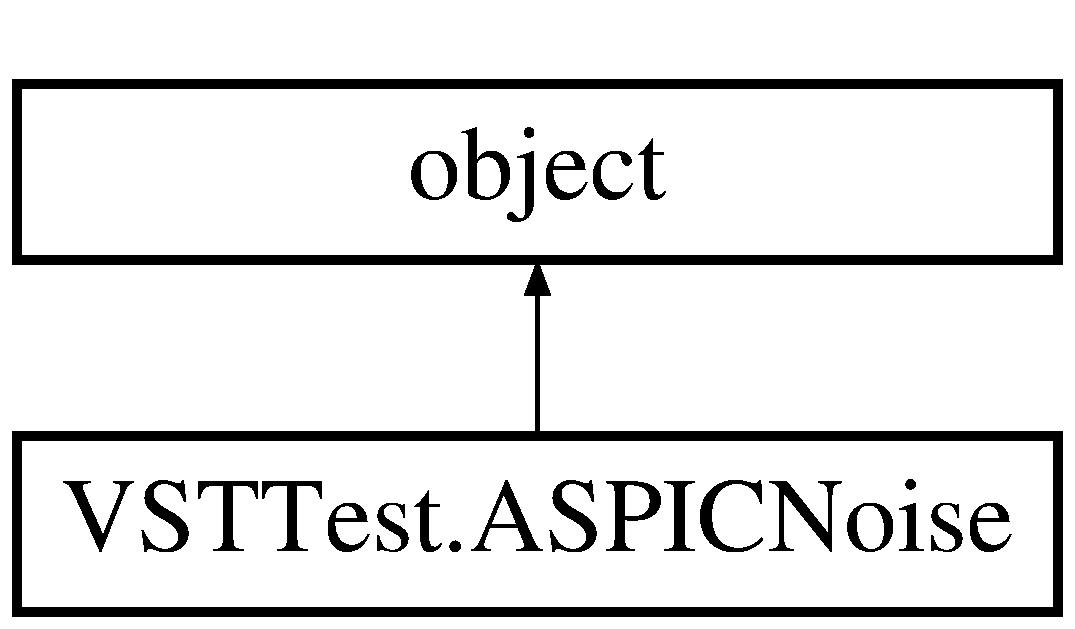
\includegraphics[height=2.000000cm]{class_v_s_t_test_1_1_a_s_p_i_c_noise}
\end{center}
\end{figure}
\subsection*{Public Member Functions}
\begin{DoxyCompactItemize}
\item 
def \hyperlink{class_v_s_t_test_1_1_a_s_p_i_c_noise_adbdd35857b4e3814cb46e18099835b13}{\+\_\+\+\_\+init\+\_\+\+\_\+} (self)
\begin{DoxyCompactList}\small\item\em Initialize minimum required variables for test list. \end{DoxyCompactList}\item 
def \hyperlink{class_v_s_t_test_1_1_a_s_p_i_c_noise_a6111fa01f3ab4e5108594ef967dd304a}{run\+Test} (self)
\begin{DoxyCompactList}\small\item\em Run the test, save output to state variables. \end{DoxyCompactList}\item 
def \hyperlink{class_v_s_t_test_1_1_a_s_p_i_c_noise_a17fb047a564da4c19572f8e3e3942687}{summarize} (self, summary)
\begin{DoxyCompactList}\small\item\em Summarize the test results for the cover page of the report. \end{DoxyCompactList}\item 
def \hyperlink{class_v_s_t_test_1_1_a_s_p_i_c_noise_a8c19116ee5a9c085973a299ec4cd3406}{report} (self, pdf)
\begin{DoxyCompactList}\small\item\em generate this test\textquotesingle{}s page in the P\+DF report. \end{DoxyCompactList}\end{DoxyCompactItemize}


\subsection{Detailed Description}
Measure noise distribution in A\+S\+P\+I\+Cs for the unclamped, clamped, and reset cases. 



\subsection{Constructor \& Destructor Documentation}
\index{V\+S\+T\+Test\+::\+A\+S\+P\+I\+C\+Noise@{V\+S\+T\+Test\+::\+A\+S\+P\+I\+C\+Noise}!\+\_\+\+\_\+init\+\_\+\+\_\+@{\+\_\+\+\_\+init\+\_\+\+\_\+}}
\index{\+\_\+\+\_\+init\+\_\+\+\_\+@{\+\_\+\+\_\+init\+\_\+\+\_\+}!V\+S\+T\+Test\+::\+A\+S\+P\+I\+C\+Noise@{V\+S\+T\+Test\+::\+A\+S\+P\+I\+C\+Noise}}
\subsubsection[{\texorpdfstring{\+\_\+\+\_\+init\+\_\+\+\_\+(self)}{__init__(self)}}]{\setlength{\rightskip}{0pt plus 5cm}def V\+S\+T\+Test.\+A\+S\+P\+I\+C\+Noise.\+\_\+\+\_\+init\+\_\+\+\_\+ (
\begin{DoxyParamCaption}
\item[{}]{self}
\end{DoxyParamCaption}
)}\hypertarget{class_v_s_t_test_1_1_a_s_p_i_c_noise_adbdd35857b4e3814cb46e18099835b13}{}\label{class_v_s_t_test_1_1_a_s_p_i_c_noise_adbdd35857b4e3814cb46e18099835b13}


Initialize minimum required variables for test list. 



\subsection{Member Function Documentation}
\index{V\+S\+T\+Test\+::\+A\+S\+P\+I\+C\+Noise@{V\+S\+T\+Test\+::\+A\+S\+P\+I\+C\+Noise}!report@{report}}
\index{report@{report}!V\+S\+T\+Test\+::\+A\+S\+P\+I\+C\+Noise@{V\+S\+T\+Test\+::\+A\+S\+P\+I\+C\+Noise}}
\subsubsection[{\texorpdfstring{report(self, pdf)}{report(self, pdf)}}]{\setlength{\rightskip}{0pt plus 5cm}def V\+S\+T\+Test.\+A\+S\+P\+I\+C\+Noise.\+report (
\begin{DoxyParamCaption}
\item[{}]{self, }
\item[{}]{pdf}
\end{DoxyParamCaption}
)}\hypertarget{class_v_s_t_test_1_1_a_s_p_i_c_noise_a8c19116ee5a9c085973a299ec4cd3406}{}\label{class_v_s_t_test_1_1_a_s_p_i_c_noise_a8c19116ee5a9c085973a299ec4cd3406}


generate this test\textquotesingle{}s page in the P\+DF report. 


\begin{DoxyParams}{Parameters}
{\em pdf} & pyfpdf-\/compatible P\+DF object. \\
\hline
\end{DoxyParams}
\index{V\+S\+T\+Test\+::\+A\+S\+P\+I\+C\+Noise@{V\+S\+T\+Test\+::\+A\+S\+P\+I\+C\+Noise}!run\+Test@{run\+Test}}
\index{run\+Test@{run\+Test}!V\+S\+T\+Test\+::\+A\+S\+P\+I\+C\+Noise@{V\+S\+T\+Test\+::\+A\+S\+P\+I\+C\+Noise}}
\subsubsection[{\texorpdfstring{run\+Test(self)}{runTest(self)}}]{\setlength{\rightskip}{0pt plus 5cm}def V\+S\+T\+Test.\+A\+S\+P\+I\+C\+Noise.\+run\+Test (
\begin{DoxyParamCaption}
\item[{}]{self}
\end{DoxyParamCaption}
)}\hypertarget{class_v_s_t_test_1_1_a_s_p_i_c_noise_a6111fa01f3ab4e5108594ef967dd304a}{}\label{class_v_s_t_test_1_1_a_s_p_i_c_noise_a6111fa01f3ab4e5108594ef967dd304a}


Run the test, save output to state variables. 

\index{V\+S\+T\+Test\+::\+A\+S\+P\+I\+C\+Noise@{V\+S\+T\+Test\+::\+A\+S\+P\+I\+C\+Noise}!summarize@{summarize}}
\index{summarize@{summarize}!V\+S\+T\+Test\+::\+A\+S\+P\+I\+C\+Noise@{V\+S\+T\+Test\+::\+A\+S\+P\+I\+C\+Noise}}
\subsubsection[{\texorpdfstring{summarize(self, summary)}{summarize(self, summary)}}]{\setlength{\rightskip}{0pt plus 5cm}def V\+S\+T\+Test.\+A\+S\+P\+I\+C\+Noise.\+summarize (
\begin{DoxyParamCaption}
\item[{}]{self, }
\item[{}]{summary}
\end{DoxyParamCaption}
)}\hypertarget{class_v_s_t_test_1_1_a_s_p_i_c_noise_a17fb047a564da4c19572f8e3e3942687}{}\label{class_v_s_t_test_1_1_a_s_p_i_c_noise_a17fb047a564da4c19572f8e3e3942687}


Summarize the test results for the cover page of the report. 


\begin{DoxyParams}{Parameters}
{\em summary} & \hyperlink{class_v_s_t_test_1_1_summary}{Summary} obejct passed from Functional\+Test() \\
\hline
\end{DoxyParams}


The documentation for this class was generated from the following file\+:\begin{DoxyCompactItemize}
\item 
\hyperlink{_v_s_t_test_8py}{V\+S\+T\+Test.\+py}\end{DoxyCompactItemize}

\hypertarget{class_w_r_e_b_test_1_1_a_s_p_i_c_noise}{}\section{W\+R\+E\+B\+Test.\+A\+S\+P\+I\+C\+Noise Class Reference}
\label{class_w_r_e_b_test_1_1_a_s_p_i_c_noise}\index{W\+R\+E\+B\+Test.\+A\+S\+P\+I\+C\+Noise@{W\+R\+E\+B\+Test.\+A\+S\+P\+I\+C\+Noise}}


Measure noise distribution in A\+S\+P\+I\+Cs for the unclamped, clamped, and reset cases.  


Inheritance diagram for W\+R\+E\+B\+Test.\+A\+S\+P\+I\+C\+Noise\+:\begin{figure}[H]
\begin{center}
\leavevmode
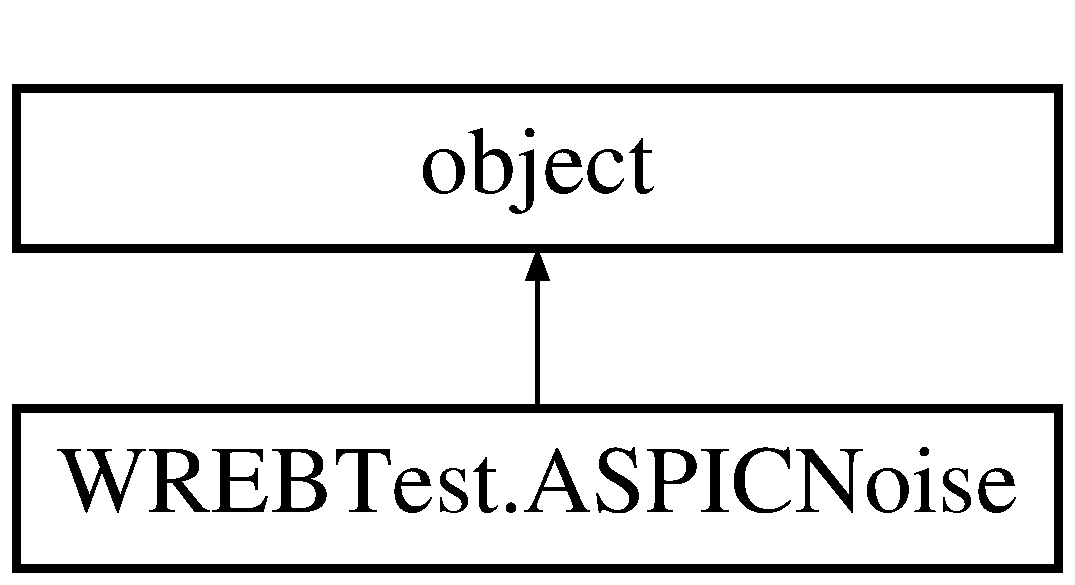
\includegraphics[height=2.000000cm]{class_w_r_e_b_test_1_1_a_s_p_i_c_noise}
\end{center}
\end{figure}
\subsection*{Public Member Functions}
\begin{DoxyCompactItemize}
\item 
def \hyperlink{class_w_r_e_b_test_1_1_a_s_p_i_c_noise_aeba1015afa34a9e7a910cea0f29e8c3d}{\+\_\+\+\_\+init\+\_\+\+\_\+} (self)
\begin{DoxyCompactList}\small\item\em Initialize minimum required variables for test list. \end{DoxyCompactList}\item 
def \hyperlink{class_w_r_e_b_test_1_1_a_s_p_i_c_noise_a19e29e14fffdf4e68138cbdfcc163239}{run\+Test} (self)
\begin{DoxyCompactList}\small\item\em Run the test, save output to state variables. \end{DoxyCompactList}\item 
def \hyperlink{class_w_r_e_b_test_1_1_a_s_p_i_c_noise_ad62fb0b9da2f0ce945d87c39bc6b21ec}{summarize} (self, summary)
\begin{DoxyCompactList}\small\item\em Summarize the test results for the cover page of the report. \end{DoxyCompactList}\item 
def \hyperlink{class_w_r_e_b_test_1_1_a_s_p_i_c_noise_afd7290484d947bfc92799c868ab27d98}{report} (self, pdf)
\begin{DoxyCompactList}\small\item\em generate this test\textquotesingle{}s page in the P\+DF report. \end{DoxyCompactList}\end{DoxyCompactItemize}


\subsection{Detailed Description}
Measure noise distribution in A\+S\+P\+I\+Cs for the unclamped, clamped, and reset cases. 



\subsection{Constructor \& Destructor Documentation}
\index{W\+R\+E\+B\+Test\+::\+A\+S\+P\+I\+C\+Noise@{W\+R\+E\+B\+Test\+::\+A\+S\+P\+I\+C\+Noise}!\+\_\+\+\_\+init\+\_\+\+\_\+@{\+\_\+\+\_\+init\+\_\+\+\_\+}}
\index{\+\_\+\+\_\+init\+\_\+\+\_\+@{\+\_\+\+\_\+init\+\_\+\+\_\+}!W\+R\+E\+B\+Test\+::\+A\+S\+P\+I\+C\+Noise@{W\+R\+E\+B\+Test\+::\+A\+S\+P\+I\+C\+Noise}}
\subsubsection[{\texorpdfstring{\+\_\+\+\_\+init\+\_\+\+\_\+(self)}{__init__(self)}}]{\setlength{\rightskip}{0pt plus 5cm}def W\+R\+E\+B\+Test.\+A\+S\+P\+I\+C\+Noise.\+\_\+\+\_\+init\+\_\+\+\_\+ (
\begin{DoxyParamCaption}
\item[{}]{self}
\end{DoxyParamCaption}
)}\hypertarget{class_w_r_e_b_test_1_1_a_s_p_i_c_noise_aeba1015afa34a9e7a910cea0f29e8c3d}{}\label{class_w_r_e_b_test_1_1_a_s_p_i_c_noise_aeba1015afa34a9e7a910cea0f29e8c3d}


Initialize minimum required variables for test list. 



\subsection{Member Function Documentation}
\index{W\+R\+E\+B\+Test\+::\+A\+S\+P\+I\+C\+Noise@{W\+R\+E\+B\+Test\+::\+A\+S\+P\+I\+C\+Noise}!report@{report}}
\index{report@{report}!W\+R\+E\+B\+Test\+::\+A\+S\+P\+I\+C\+Noise@{W\+R\+E\+B\+Test\+::\+A\+S\+P\+I\+C\+Noise}}
\subsubsection[{\texorpdfstring{report(self, pdf)}{report(self, pdf)}}]{\setlength{\rightskip}{0pt plus 5cm}def W\+R\+E\+B\+Test.\+A\+S\+P\+I\+C\+Noise.\+report (
\begin{DoxyParamCaption}
\item[{}]{self, }
\item[{}]{pdf}
\end{DoxyParamCaption}
)}\hypertarget{class_w_r_e_b_test_1_1_a_s_p_i_c_noise_afd7290484d947bfc92799c868ab27d98}{}\label{class_w_r_e_b_test_1_1_a_s_p_i_c_noise_afd7290484d947bfc92799c868ab27d98}


generate this test\textquotesingle{}s page in the P\+DF report. 


\begin{DoxyParams}{Parameters}
{\em pdf} & pyfpdf-\/compatible P\+DF object. \\
\hline
\end{DoxyParams}
\index{W\+R\+E\+B\+Test\+::\+A\+S\+P\+I\+C\+Noise@{W\+R\+E\+B\+Test\+::\+A\+S\+P\+I\+C\+Noise}!run\+Test@{run\+Test}}
\index{run\+Test@{run\+Test}!W\+R\+E\+B\+Test\+::\+A\+S\+P\+I\+C\+Noise@{W\+R\+E\+B\+Test\+::\+A\+S\+P\+I\+C\+Noise}}
\subsubsection[{\texorpdfstring{run\+Test(self)}{runTest(self)}}]{\setlength{\rightskip}{0pt plus 5cm}def W\+R\+E\+B\+Test.\+A\+S\+P\+I\+C\+Noise.\+run\+Test (
\begin{DoxyParamCaption}
\item[{}]{self}
\end{DoxyParamCaption}
)}\hypertarget{class_w_r_e_b_test_1_1_a_s_p_i_c_noise_a19e29e14fffdf4e68138cbdfcc163239}{}\label{class_w_r_e_b_test_1_1_a_s_p_i_c_noise_a19e29e14fffdf4e68138cbdfcc163239}


Run the test, save output to state variables. 

\index{W\+R\+E\+B\+Test\+::\+A\+S\+P\+I\+C\+Noise@{W\+R\+E\+B\+Test\+::\+A\+S\+P\+I\+C\+Noise}!summarize@{summarize}}
\index{summarize@{summarize}!W\+R\+E\+B\+Test\+::\+A\+S\+P\+I\+C\+Noise@{W\+R\+E\+B\+Test\+::\+A\+S\+P\+I\+C\+Noise}}
\subsubsection[{\texorpdfstring{summarize(self, summary)}{summarize(self, summary)}}]{\setlength{\rightskip}{0pt plus 5cm}def W\+R\+E\+B\+Test.\+A\+S\+P\+I\+C\+Noise.\+summarize (
\begin{DoxyParamCaption}
\item[{}]{self, }
\item[{}]{summary}
\end{DoxyParamCaption}
)}\hypertarget{class_w_r_e_b_test_1_1_a_s_p_i_c_noise_ad62fb0b9da2f0ce945d87c39bc6b21ec}{}\label{class_w_r_e_b_test_1_1_a_s_p_i_c_noise_ad62fb0b9da2f0ce945d87c39bc6b21ec}


Summarize the test results for the cover page of the report. 


\begin{DoxyParams}{Parameters}
{\em summary} & \hyperlink{class_w_r_e_b_test_1_1_summary}{Summary} obejct passed from Functional\+Test() \\
\hline
\end{DoxyParams}


The documentation for this class was generated from the following file\+:\begin{DoxyCompactItemize}
\item 
\hyperlink{_w_r_e_b_test_8py}{W\+R\+E\+B\+Test.\+py}\end{DoxyCompactItemize}

\hypertarget{classdeprecated_1_1_board_select}{}\section{deprecated.\+Board\+Select Class Reference}
\label{classdeprecated_1_1_board_select}\index{deprecated.\+Board\+Select@{deprecated.\+Board\+Select}}


Dialog-\/based G\+UI for displaying test progress and navigating options.  


Inheritance diagram for deprecated.\+Board\+Select\+:\begin{figure}[H]
\begin{center}
\leavevmode
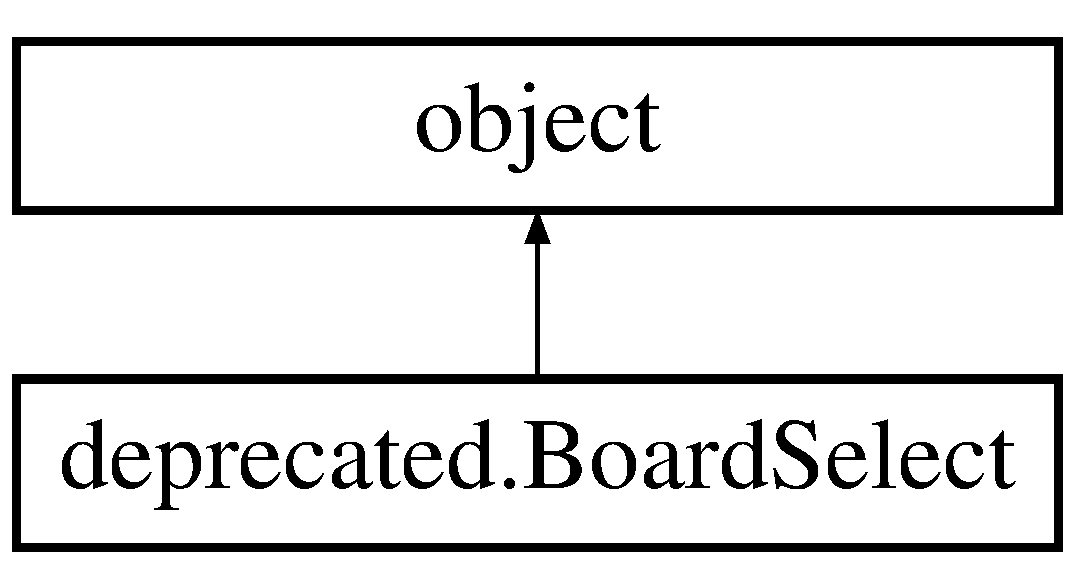
\includegraphics[height=2.000000cm]{classdeprecated_1_1_board_select}
\end{center}
\end{figure}
\subsection*{Public Member Functions}
\begin{DoxyCompactItemize}
\item 
def \hyperlink{classdeprecated_1_1_board_select_aab94c6c85115ea66c47d0158dfca5659}{\+\_\+\+\_\+init\+\_\+\+\_\+} (self)
\begin{DoxyCompactList}\small\item\em Start the dialog. \end{DoxyCompactList}\item 
def \hyperlink{classdeprecated_1_1_board_select_a00a559c89aa9a4c381a2036ddaebae3b}{start\+Menu} (self)\hypertarget{classdeprecated_1_1_board_select_a00a559c89aa9a4c381a2036ddaebae3b}{}\label{classdeprecated_1_1_board_select_a00a559c89aa9a4c381a2036ddaebae3b}

\begin{DoxyCompactList}\small\item\em Initial board selection menu. \end{DoxyCompactList}\end{DoxyCompactItemize}


\subsection{Detailed Description}
Dialog-\/based G\+UI for displaying test progress and navigating options. 



\subsection{Constructor \& Destructor Documentation}
\index{deprecated\+::\+Board\+Select@{deprecated\+::\+Board\+Select}!\+\_\+\+\_\+init\+\_\+\+\_\+@{\+\_\+\+\_\+init\+\_\+\+\_\+}}
\index{\+\_\+\+\_\+init\+\_\+\+\_\+@{\+\_\+\+\_\+init\+\_\+\+\_\+}!deprecated\+::\+Board\+Select@{deprecated\+::\+Board\+Select}}
\subsubsection[{\texorpdfstring{\+\_\+\+\_\+init\+\_\+\+\_\+(self)}{__init__(self)}}]{\setlength{\rightskip}{0pt plus 5cm}def deprecated.\+Board\+Select.\+\_\+\+\_\+init\+\_\+\+\_\+ (
\begin{DoxyParamCaption}
\item[{}]{self}
\end{DoxyParamCaption}
)}\hypertarget{classdeprecated_1_1_board_select_aab94c6c85115ea66c47d0158dfca5659}{}\label{classdeprecated_1_1_board_select_aab94c6c85115ea66c47d0158dfca5659}


Start the dialog. 



The documentation for this class was generated from the following file\+:\begin{DoxyCompactItemize}
\item 
deprecated.\+R\+E\+B\+Test.\+py\end{DoxyCompactItemize}

\hypertarget{class_g_r_e_b_test_1_1_channel_test}{}\section{G\+R\+E\+B\+Test.\+Channel\+Test Class Reference}
\label{class_g_r_e_b_test_1_1_channel_test}\index{G\+R\+E\+B\+Test.\+Channel\+Test@{G\+R\+E\+B\+Test.\+Channel\+Test}}


Tests number of communicable channels available to the board.  


Inheritance diagram for G\+R\+E\+B\+Test.\+Channel\+Test\+:\begin{figure}[H]
\begin{center}
\leavevmode
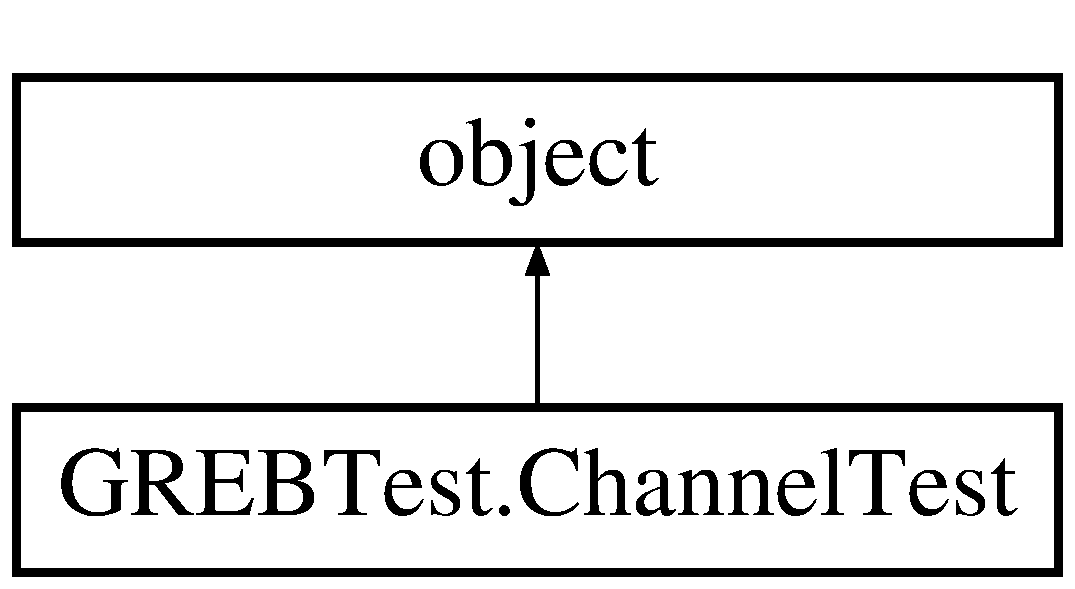
\includegraphics[height=2.000000cm]{class_g_r_e_b_test_1_1_channel_test}
\end{center}
\end{figure}
\subsection*{Public Member Functions}
\begin{DoxyCompactItemize}
\item 
def \hyperlink{class_g_r_e_b_test_1_1_channel_test_aa01ae906573e0a056b12b23acb1e3039}{\+\_\+\+\_\+init\+\_\+\+\_\+} (self)
\begin{DoxyCompactList}\small\item\em Initialize minimum required variables for test list. \end{DoxyCompactList}\item 
def \hyperlink{class_g_r_e_b_test_1_1_channel_test_ad3b83c5d4ba92385d6c9a0b41971cb98}{run\+Test} (self)
\begin{DoxyCompactList}\small\item\em Run the test, save output to state variables. \end{DoxyCompactList}\item 
def \hyperlink{class_g_r_e_b_test_1_1_channel_test_a7256a7c8f9aad2de49575381bebb099b}{summarize} (self, summary)
\begin{DoxyCompactList}\small\item\em Summarize the test results for the cover page of the report. \end{DoxyCompactList}\item 
def \hyperlink{class_g_r_e_b_test_1_1_channel_test_a2741ea419616e82f0f2e845c9f11d66f}{report} (self, pdf, report\+Path)
\begin{DoxyCompactList}\small\item\em generate this test\textquotesingle{}s page in the P\+DF report. \end{DoxyCompactList}\end{DoxyCompactItemize}


\subsection{Detailed Description}
Tests number of communicable channels available to the board. 



\subsection{Constructor \& Destructor Documentation}
\index{G\+R\+E\+B\+Test\+::\+Channel\+Test@{G\+R\+E\+B\+Test\+::\+Channel\+Test}!\+\_\+\+\_\+init\+\_\+\+\_\+@{\+\_\+\+\_\+init\+\_\+\+\_\+}}
\index{\+\_\+\+\_\+init\+\_\+\+\_\+@{\+\_\+\+\_\+init\+\_\+\+\_\+}!G\+R\+E\+B\+Test\+::\+Channel\+Test@{G\+R\+E\+B\+Test\+::\+Channel\+Test}}
\subsubsection[{\texorpdfstring{\+\_\+\+\_\+init\+\_\+\+\_\+(self)}{__init__(self)}}]{\setlength{\rightskip}{0pt plus 5cm}def G\+R\+E\+B\+Test.\+Channel\+Test.\+\_\+\+\_\+init\+\_\+\+\_\+ (
\begin{DoxyParamCaption}
\item[{}]{self}
\end{DoxyParamCaption}
)}\hypertarget{class_g_r_e_b_test_1_1_channel_test_aa01ae906573e0a056b12b23acb1e3039}{}\label{class_g_r_e_b_test_1_1_channel_test_aa01ae906573e0a056b12b23acb1e3039}


Initialize minimum required variables for test list. 



\subsection{Member Function Documentation}
\index{G\+R\+E\+B\+Test\+::\+Channel\+Test@{G\+R\+E\+B\+Test\+::\+Channel\+Test}!report@{report}}
\index{report@{report}!G\+R\+E\+B\+Test\+::\+Channel\+Test@{G\+R\+E\+B\+Test\+::\+Channel\+Test}}
\subsubsection[{\texorpdfstring{report(self, pdf, report\+Path)}{report(self, pdf, reportPath)}}]{\setlength{\rightskip}{0pt plus 5cm}def G\+R\+E\+B\+Test.\+Channel\+Test.\+report (
\begin{DoxyParamCaption}
\item[{}]{self, }
\item[{}]{pdf, }
\item[{}]{report\+Path}
\end{DoxyParamCaption}
)}\hypertarget{class_g_r_e_b_test_1_1_channel_test_a2741ea419616e82f0f2e845c9f11d66f}{}\label{class_g_r_e_b_test_1_1_channel_test_a2741ea419616e82f0f2e845c9f11d66f}


generate this test\textquotesingle{}s page in the P\+DF report. 


\begin{DoxyParams}{Parameters}
{\em pdf} & pyfpdf-\/compatible P\+DF object. \\
\hline
{\em report\+Path} & Path of directory containing the pdf report \\
\hline
\end{DoxyParams}
\index{G\+R\+E\+B\+Test\+::\+Channel\+Test@{G\+R\+E\+B\+Test\+::\+Channel\+Test}!run\+Test@{run\+Test}}
\index{run\+Test@{run\+Test}!G\+R\+E\+B\+Test\+::\+Channel\+Test@{G\+R\+E\+B\+Test\+::\+Channel\+Test}}
\subsubsection[{\texorpdfstring{run\+Test(self)}{runTest(self)}}]{\setlength{\rightskip}{0pt plus 5cm}def G\+R\+E\+B\+Test.\+Channel\+Test.\+run\+Test (
\begin{DoxyParamCaption}
\item[{}]{self}
\end{DoxyParamCaption}
)}\hypertarget{class_g_r_e_b_test_1_1_channel_test_ad3b83c5d4ba92385d6c9a0b41971cb98}{}\label{class_g_r_e_b_test_1_1_channel_test_ad3b83c5d4ba92385d6c9a0b41971cb98}


Run the test, save output to state variables. 

\index{G\+R\+E\+B\+Test\+::\+Channel\+Test@{G\+R\+E\+B\+Test\+::\+Channel\+Test}!summarize@{summarize}}
\index{summarize@{summarize}!G\+R\+E\+B\+Test\+::\+Channel\+Test@{G\+R\+E\+B\+Test\+::\+Channel\+Test}}
\subsubsection[{\texorpdfstring{summarize(self, summary)}{summarize(self, summary)}}]{\setlength{\rightskip}{0pt plus 5cm}def G\+R\+E\+B\+Test.\+Channel\+Test.\+summarize (
\begin{DoxyParamCaption}
\item[{}]{self, }
\item[{}]{summary}
\end{DoxyParamCaption}
)}\hypertarget{class_g_r_e_b_test_1_1_channel_test_a7256a7c8f9aad2de49575381bebb099b}{}\label{class_g_r_e_b_test_1_1_channel_test_a7256a7c8f9aad2de49575381bebb099b}


Summarize the test results for the cover page of the report. 


\begin{DoxyParams}{Parameters}
{\em summary} & \hyperlink{class_g_r_e_b_test_1_1_summary}{Summary} obejct passed from Functional\+Test() \\
\hline
\end{DoxyParams}


The documentation for this class was generated from the following file\+:\begin{DoxyCompactItemize}
\item 
\hyperlink{_g_r_e_b_test_8py}{G\+R\+E\+B\+Test.\+py}\end{DoxyCompactItemize}

\hypertarget{class_w_r_e_b_test_1_1_channel_test}{}\section{W\+R\+E\+B\+Test.\+Channel\+Test Class Reference}
\label{class_w_r_e_b_test_1_1_channel_test}\index{W\+R\+E\+B\+Test.\+Channel\+Test@{W\+R\+E\+B\+Test.\+Channel\+Test}}


Tests number of communicable channels available to the board.  


Inheritance diagram for W\+R\+E\+B\+Test.\+Channel\+Test\+:\begin{figure}[H]
\begin{center}
\leavevmode
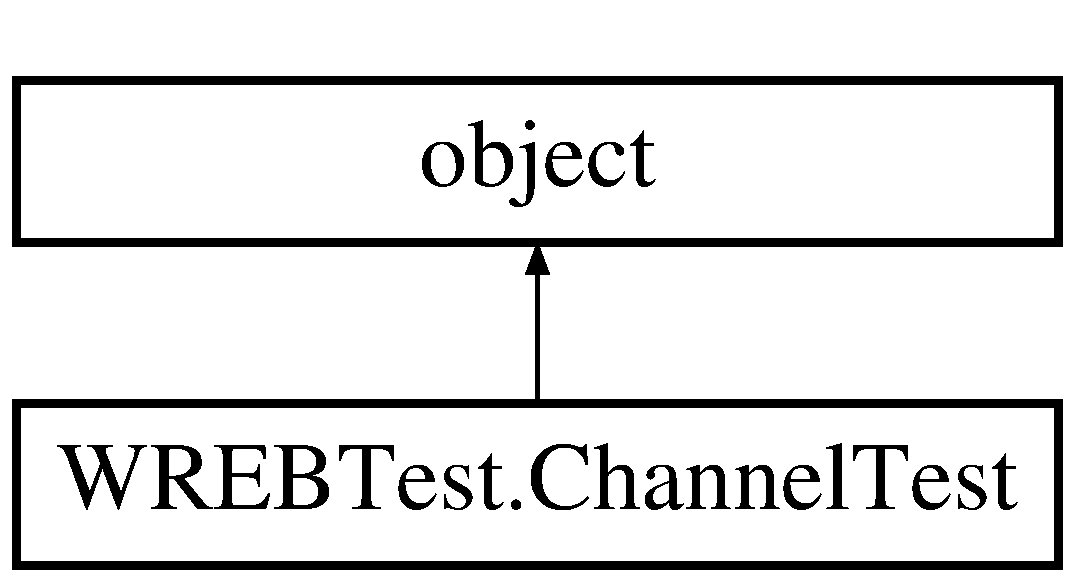
\includegraphics[height=2.000000cm]{class_w_r_e_b_test_1_1_channel_test}
\end{center}
\end{figure}
\subsection*{Public Member Functions}
\begin{DoxyCompactItemize}
\item 
def \hyperlink{class_w_r_e_b_test_1_1_channel_test_a52771dc0fe0c01373ebd9857bdaa45b1}{\+\_\+\+\_\+init\+\_\+\+\_\+} (self)
\begin{DoxyCompactList}\small\item\em Initialize minimum required variables for test list. \end{DoxyCompactList}\item 
def \hyperlink{class_w_r_e_b_test_1_1_channel_test_aad063c6ec4ec9b834f3799e1aa5d2d32}{run\+Test} (self)
\begin{DoxyCompactList}\small\item\em Run the test, save output to state variables. \end{DoxyCompactList}\item 
def \hyperlink{class_w_r_e_b_test_1_1_channel_test_a298393ff7375dbd2928d83b3fa1448c6}{summarize} (self, summary)
\begin{DoxyCompactList}\small\item\em Summarize the test results for the cover page of the report. \end{DoxyCompactList}\item 
def \hyperlink{class_w_r_e_b_test_1_1_channel_test_a0d929d9ab91f224afa432d3e461a3575}{report} (self, pdf, report\+Path)
\begin{DoxyCompactList}\small\item\em generate this test\textquotesingle{}s page in the P\+DF report. \end{DoxyCompactList}\end{DoxyCompactItemize}


\subsection{Detailed Description}
Tests number of communicable channels available to the board. 



\subsection{Constructor \& Destructor Documentation}
\index{W\+R\+E\+B\+Test\+::\+Channel\+Test@{W\+R\+E\+B\+Test\+::\+Channel\+Test}!\+\_\+\+\_\+init\+\_\+\+\_\+@{\+\_\+\+\_\+init\+\_\+\+\_\+}}
\index{\+\_\+\+\_\+init\+\_\+\+\_\+@{\+\_\+\+\_\+init\+\_\+\+\_\+}!W\+R\+E\+B\+Test\+::\+Channel\+Test@{W\+R\+E\+B\+Test\+::\+Channel\+Test}}
\subsubsection[{\texorpdfstring{\+\_\+\+\_\+init\+\_\+\+\_\+(self)}{__init__(self)}}]{\setlength{\rightskip}{0pt plus 5cm}def W\+R\+E\+B\+Test.\+Channel\+Test.\+\_\+\+\_\+init\+\_\+\+\_\+ (
\begin{DoxyParamCaption}
\item[{}]{self}
\end{DoxyParamCaption}
)}\hypertarget{class_w_r_e_b_test_1_1_channel_test_a52771dc0fe0c01373ebd9857bdaa45b1}{}\label{class_w_r_e_b_test_1_1_channel_test_a52771dc0fe0c01373ebd9857bdaa45b1}


Initialize minimum required variables for test list. 



\subsection{Member Function Documentation}
\index{W\+R\+E\+B\+Test\+::\+Channel\+Test@{W\+R\+E\+B\+Test\+::\+Channel\+Test}!report@{report}}
\index{report@{report}!W\+R\+E\+B\+Test\+::\+Channel\+Test@{W\+R\+E\+B\+Test\+::\+Channel\+Test}}
\subsubsection[{\texorpdfstring{report(self, pdf, report\+Path)}{report(self, pdf, reportPath)}}]{\setlength{\rightskip}{0pt plus 5cm}def W\+R\+E\+B\+Test.\+Channel\+Test.\+report (
\begin{DoxyParamCaption}
\item[{}]{self, }
\item[{}]{pdf, }
\item[{}]{report\+Path}
\end{DoxyParamCaption}
)}\hypertarget{class_w_r_e_b_test_1_1_channel_test_a0d929d9ab91f224afa432d3e461a3575}{}\label{class_w_r_e_b_test_1_1_channel_test_a0d929d9ab91f224afa432d3e461a3575}


generate this test\textquotesingle{}s page in the P\+DF report. 


\begin{DoxyParams}{Parameters}
{\em pdf} & pyfpdf-\/compatible P\+DF object. \\
\hline
{\em report\+Path} & Path of directory containing the pdf report \\
\hline
\end{DoxyParams}
\index{W\+R\+E\+B\+Test\+::\+Channel\+Test@{W\+R\+E\+B\+Test\+::\+Channel\+Test}!run\+Test@{run\+Test}}
\index{run\+Test@{run\+Test}!W\+R\+E\+B\+Test\+::\+Channel\+Test@{W\+R\+E\+B\+Test\+::\+Channel\+Test}}
\subsubsection[{\texorpdfstring{run\+Test(self)}{runTest(self)}}]{\setlength{\rightskip}{0pt plus 5cm}def W\+R\+E\+B\+Test.\+Channel\+Test.\+run\+Test (
\begin{DoxyParamCaption}
\item[{}]{self}
\end{DoxyParamCaption}
)}\hypertarget{class_w_r_e_b_test_1_1_channel_test_aad063c6ec4ec9b834f3799e1aa5d2d32}{}\label{class_w_r_e_b_test_1_1_channel_test_aad063c6ec4ec9b834f3799e1aa5d2d32}


Run the test, save output to state variables. 

\index{W\+R\+E\+B\+Test\+::\+Channel\+Test@{W\+R\+E\+B\+Test\+::\+Channel\+Test}!summarize@{summarize}}
\index{summarize@{summarize}!W\+R\+E\+B\+Test\+::\+Channel\+Test@{W\+R\+E\+B\+Test\+::\+Channel\+Test}}
\subsubsection[{\texorpdfstring{summarize(self, summary)}{summarize(self, summary)}}]{\setlength{\rightskip}{0pt plus 5cm}def W\+R\+E\+B\+Test.\+Channel\+Test.\+summarize (
\begin{DoxyParamCaption}
\item[{}]{self, }
\item[{}]{summary}
\end{DoxyParamCaption}
)}\hypertarget{class_w_r_e_b_test_1_1_channel_test_a298393ff7375dbd2928d83b3fa1448c6}{}\label{class_w_r_e_b_test_1_1_channel_test_a298393ff7375dbd2928d83b3fa1448c6}


Summarize the test results for the cover page of the report. 


\begin{DoxyParams}{Parameters}
{\em summary} & \hyperlink{class_w_r_e_b_test_1_1_summary}{Summary} obejct passed from Functional\+Test() \\
\hline
\end{DoxyParams}


The documentation for this class was generated from the following file\+:\begin{DoxyCompactItemize}
\item 
\hyperlink{_w_r_e_b_test_8py}{W\+R\+E\+B\+Test.\+py}\end{DoxyCompactItemize}

\hypertarget{class_v_s_t_test_1_1_channel_test}{}\section{V\+S\+T\+Test.\+Channel\+Test Class Reference}
\label{class_v_s_t_test_1_1_channel_test}\index{V\+S\+T\+Test.\+Channel\+Test@{V\+S\+T\+Test.\+Channel\+Test}}


Tests number of communicable channels available to the board.  


Inheritance diagram for V\+S\+T\+Test.\+Channel\+Test\+:\begin{figure}[H]
\begin{center}
\leavevmode
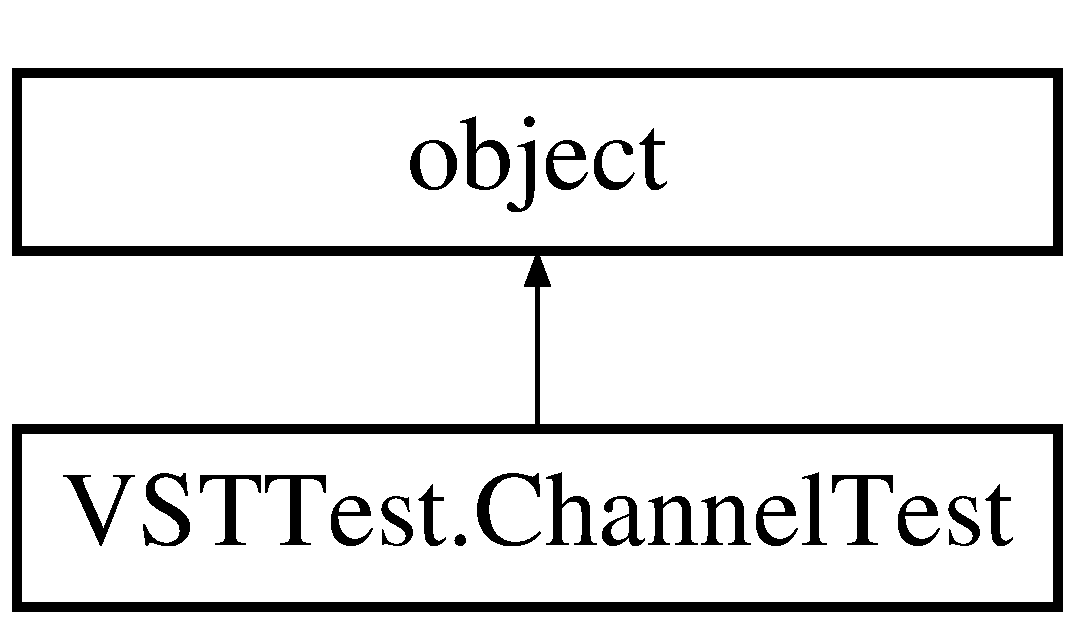
\includegraphics[height=2.000000cm]{class_v_s_t_test_1_1_channel_test}
\end{center}
\end{figure}
\subsection*{Public Member Functions}
\begin{DoxyCompactItemize}
\item 
def \hyperlink{class_v_s_t_test_1_1_channel_test_a63bf2fa1f6a019a832692102fcad7ee5}{\+\_\+\+\_\+init\+\_\+\+\_\+} (self)
\begin{DoxyCompactList}\small\item\em Initialize minimum required variables for test list. \end{DoxyCompactList}\item 
def \hyperlink{class_v_s_t_test_1_1_channel_test_a608d3ca04e5d754dd68153198d8f22a8}{run\+Test} (self)
\begin{DoxyCompactList}\small\item\em Run the test, save output to state variables. \end{DoxyCompactList}\item 
def \hyperlink{class_v_s_t_test_1_1_channel_test_a542b2fb3184ebc2a58570cabe8d558e1}{summarize} (self, summary)
\begin{DoxyCompactList}\small\item\em Summarize the test results for the cover page of the report. \end{DoxyCompactList}\item 
def \hyperlink{class_v_s_t_test_1_1_channel_test_a98fc5d455f72cafc1498e5dfc68d4328}{report} (self, pdf, report\+Path)
\begin{DoxyCompactList}\small\item\em generate this test\textquotesingle{}s page in the P\+DF report. \end{DoxyCompactList}\end{DoxyCompactItemize}


\subsection{Detailed Description}
Tests number of communicable channels available to the board. 



\subsection{Constructor \& Destructor Documentation}
\index{V\+S\+T\+Test\+::\+Channel\+Test@{V\+S\+T\+Test\+::\+Channel\+Test}!\+\_\+\+\_\+init\+\_\+\+\_\+@{\+\_\+\+\_\+init\+\_\+\+\_\+}}
\index{\+\_\+\+\_\+init\+\_\+\+\_\+@{\+\_\+\+\_\+init\+\_\+\+\_\+}!V\+S\+T\+Test\+::\+Channel\+Test@{V\+S\+T\+Test\+::\+Channel\+Test}}
\subsubsection[{\texorpdfstring{\+\_\+\+\_\+init\+\_\+\+\_\+(self)}{__init__(self)}}]{\setlength{\rightskip}{0pt plus 5cm}def V\+S\+T\+Test.\+Channel\+Test.\+\_\+\+\_\+init\+\_\+\+\_\+ (
\begin{DoxyParamCaption}
\item[{}]{self}
\end{DoxyParamCaption}
)}\hypertarget{class_v_s_t_test_1_1_channel_test_a63bf2fa1f6a019a832692102fcad7ee5}{}\label{class_v_s_t_test_1_1_channel_test_a63bf2fa1f6a019a832692102fcad7ee5}


Initialize minimum required variables for test list. 



\subsection{Member Function Documentation}
\index{V\+S\+T\+Test\+::\+Channel\+Test@{V\+S\+T\+Test\+::\+Channel\+Test}!report@{report}}
\index{report@{report}!V\+S\+T\+Test\+::\+Channel\+Test@{V\+S\+T\+Test\+::\+Channel\+Test}}
\subsubsection[{\texorpdfstring{report(self, pdf, report\+Path)}{report(self, pdf, reportPath)}}]{\setlength{\rightskip}{0pt plus 5cm}def V\+S\+T\+Test.\+Channel\+Test.\+report (
\begin{DoxyParamCaption}
\item[{}]{self, }
\item[{}]{pdf, }
\item[{}]{report\+Path}
\end{DoxyParamCaption}
)}\hypertarget{class_v_s_t_test_1_1_channel_test_a98fc5d455f72cafc1498e5dfc68d4328}{}\label{class_v_s_t_test_1_1_channel_test_a98fc5d455f72cafc1498e5dfc68d4328}


generate this test\textquotesingle{}s page in the P\+DF report. 


\begin{DoxyParams}{Parameters}
{\em pdf} & pyfpdf-\/compatible P\+DF object. \\
\hline
{\em report\+Path} & Path of directory containing the pdf report \\
\hline
\end{DoxyParams}
\index{V\+S\+T\+Test\+::\+Channel\+Test@{V\+S\+T\+Test\+::\+Channel\+Test}!run\+Test@{run\+Test}}
\index{run\+Test@{run\+Test}!V\+S\+T\+Test\+::\+Channel\+Test@{V\+S\+T\+Test\+::\+Channel\+Test}}
\subsubsection[{\texorpdfstring{run\+Test(self)}{runTest(self)}}]{\setlength{\rightskip}{0pt plus 5cm}def V\+S\+T\+Test.\+Channel\+Test.\+run\+Test (
\begin{DoxyParamCaption}
\item[{}]{self}
\end{DoxyParamCaption}
)}\hypertarget{class_v_s_t_test_1_1_channel_test_a608d3ca04e5d754dd68153198d8f22a8}{}\label{class_v_s_t_test_1_1_channel_test_a608d3ca04e5d754dd68153198d8f22a8}


Run the test, save output to state variables. 

\index{V\+S\+T\+Test\+::\+Channel\+Test@{V\+S\+T\+Test\+::\+Channel\+Test}!summarize@{summarize}}
\index{summarize@{summarize}!V\+S\+T\+Test\+::\+Channel\+Test@{V\+S\+T\+Test\+::\+Channel\+Test}}
\subsubsection[{\texorpdfstring{summarize(self, summary)}{summarize(self, summary)}}]{\setlength{\rightskip}{0pt plus 5cm}def V\+S\+T\+Test.\+Channel\+Test.\+summarize (
\begin{DoxyParamCaption}
\item[{}]{self, }
\item[{}]{summary}
\end{DoxyParamCaption}
)}\hypertarget{class_v_s_t_test_1_1_channel_test_a542b2fb3184ebc2a58570cabe8d558e1}{}\label{class_v_s_t_test_1_1_channel_test_a542b2fb3184ebc2a58570cabe8d558e1}


Summarize the test results for the cover page of the report. 


\begin{DoxyParams}{Parameters}
{\em summary} & \hyperlink{class_v_s_t_test_1_1_summary}{Summary} obejct passed from Functional\+Test() \\
\hline
\end{DoxyParams}


The documentation for this class was generated from the following file\+:\begin{DoxyCompactItemize}
\item 
\hyperlink{_v_s_t_test_8py}{V\+S\+T\+Test.\+py}\end{DoxyCompactItemize}

\hypertarget{class_w_r_e_b_test_1_1_c_s_gate}{}\section{W\+R\+E\+B\+Test.\+C\+S\+Gate Class Reference}
\label{class_w_r_e_b_test_1_1_c_s_gate}\index{W\+R\+E\+B\+Test.\+C\+S\+Gate@{W\+R\+E\+B\+Test.\+C\+S\+Gate}}


Tests the current source gate.  


Inheritance diagram for W\+R\+E\+B\+Test.\+C\+S\+Gate\+:\begin{figure}[H]
\begin{center}
\leavevmode
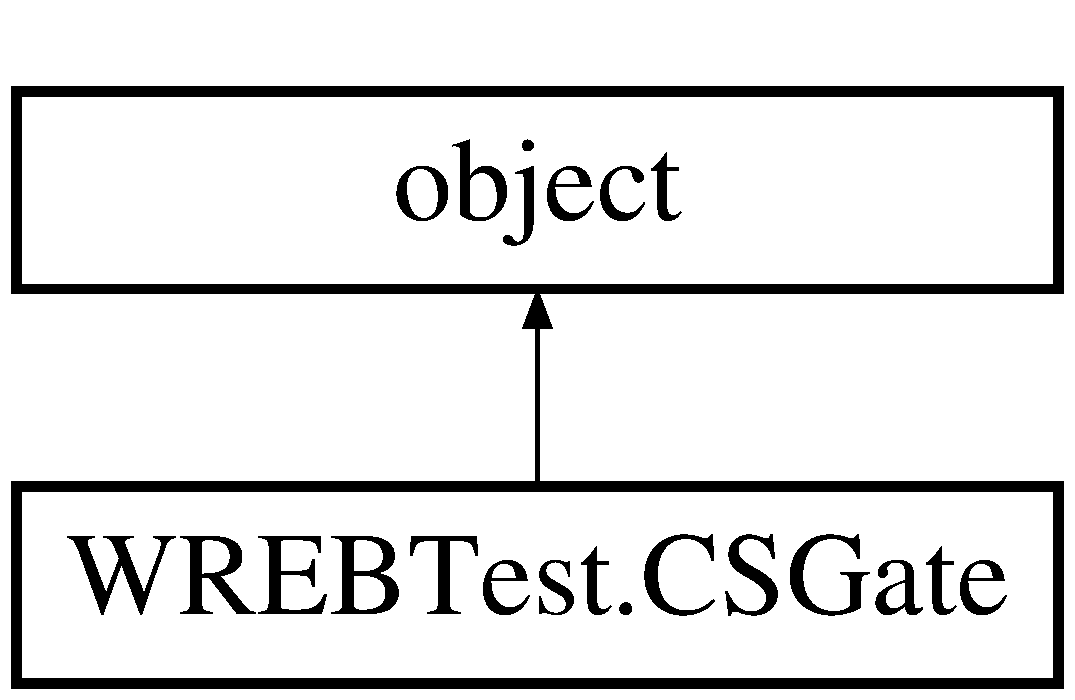
\includegraphics[height=2.000000cm]{class_w_r_e_b_test_1_1_c_s_gate}
\end{center}
\end{figure}
\subsection*{Public Member Functions}
\begin{DoxyCompactItemize}
\item 
def \hyperlink{class_w_r_e_b_test_1_1_c_s_gate_a1ef42c27062a4336a6e38153f0d63f22}{\+\_\+\+\_\+init\+\_\+\+\_\+} (self)
\begin{DoxyCompactList}\small\item\em Initialize minimum required variables for test list. \end{DoxyCompactList}\item 
def \hyperlink{class_w_r_e_b_test_1_1_c_s_gate_a2022ca5cfd0cca5dc1e68c96bee503e5}{run\+Test} (self)
\begin{DoxyCompactList}\small\item\em Run the test, save output to state variables. \end{DoxyCompactList}\item 
def \hyperlink{class_w_r_e_b_test_1_1_c_s_gate_ace80c551527bc66602b517fa0891ae55}{summarize} (self, summary)
\begin{DoxyCompactList}\small\item\em Summarize the test results for the cover page of the report. \end{DoxyCompactList}\item 
def \hyperlink{class_w_r_e_b_test_1_1_c_s_gate_a9f773280dd583a852b784ea858f52d5c}{report} (self, pdf)
\begin{DoxyCompactList}\small\item\em generate this test\textquotesingle{}s page in the P\+DF report. \end{DoxyCompactList}\end{DoxyCompactItemize}


\subsection{Detailed Description}
Tests the current source gate. 



\subsection{Constructor \& Destructor Documentation}
\index{W\+R\+E\+B\+Test\+::\+C\+S\+Gate@{W\+R\+E\+B\+Test\+::\+C\+S\+Gate}!\+\_\+\+\_\+init\+\_\+\+\_\+@{\+\_\+\+\_\+init\+\_\+\+\_\+}}
\index{\+\_\+\+\_\+init\+\_\+\+\_\+@{\+\_\+\+\_\+init\+\_\+\+\_\+}!W\+R\+E\+B\+Test\+::\+C\+S\+Gate@{W\+R\+E\+B\+Test\+::\+C\+S\+Gate}}
\subsubsection[{\texorpdfstring{\+\_\+\+\_\+init\+\_\+\+\_\+(self)}{__init__(self)}}]{\setlength{\rightskip}{0pt plus 5cm}def W\+R\+E\+B\+Test.\+C\+S\+Gate.\+\_\+\+\_\+init\+\_\+\+\_\+ (
\begin{DoxyParamCaption}
\item[{}]{self}
\end{DoxyParamCaption}
)}\hypertarget{class_w_r_e_b_test_1_1_c_s_gate_a1ef42c27062a4336a6e38153f0d63f22}{}\label{class_w_r_e_b_test_1_1_c_s_gate_a1ef42c27062a4336a6e38153f0d63f22}


Initialize minimum required variables for test list. 



\subsection{Member Function Documentation}
\index{W\+R\+E\+B\+Test\+::\+C\+S\+Gate@{W\+R\+E\+B\+Test\+::\+C\+S\+Gate}!report@{report}}
\index{report@{report}!W\+R\+E\+B\+Test\+::\+C\+S\+Gate@{W\+R\+E\+B\+Test\+::\+C\+S\+Gate}}
\subsubsection[{\texorpdfstring{report(self, pdf)}{report(self, pdf)}}]{\setlength{\rightskip}{0pt plus 5cm}def W\+R\+E\+B\+Test.\+C\+S\+Gate.\+report (
\begin{DoxyParamCaption}
\item[{}]{self, }
\item[{}]{pdf}
\end{DoxyParamCaption}
)}\hypertarget{class_w_r_e_b_test_1_1_c_s_gate_a9f773280dd583a852b784ea858f52d5c}{}\label{class_w_r_e_b_test_1_1_c_s_gate_a9f773280dd583a852b784ea858f52d5c}


generate this test\textquotesingle{}s page in the P\+DF report. 


\begin{DoxyParams}{Parameters}
{\em pdf} & pyfpdf-\/compatible P\+DF object. \\
\hline
\end{DoxyParams}
\index{W\+R\+E\+B\+Test\+::\+C\+S\+Gate@{W\+R\+E\+B\+Test\+::\+C\+S\+Gate}!run\+Test@{run\+Test}}
\index{run\+Test@{run\+Test}!W\+R\+E\+B\+Test\+::\+C\+S\+Gate@{W\+R\+E\+B\+Test\+::\+C\+S\+Gate}}
\subsubsection[{\texorpdfstring{run\+Test(self)}{runTest(self)}}]{\setlength{\rightskip}{0pt plus 5cm}def W\+R\+E\+B\+Test.\+C\+S\+Gate.\+run\+Test (
\begin{DoxyParamCaption}
\item[{}]{self}
\end{DoxyParamCaption}
)}\hypertarget{class_w_r_e_b_test_1_1_c_s_gate_a2022ca5cfd0cca5dc1e68c96bee503e5}{}\label{class_w_r_e_b_test_1_1_c_s_gate_a2022ca5cfd0cca5dc1e68c96bee503e5}


Run the test, save output to state variables. 

\index{W\+R\+E\+B\+Test\+::\+C\+S\+Gate@{W\+R\+E\+B\+Test\+::\+C\+S\+Gate}!summarize@{summarize}}
\index{summarize@{summarize}!W\+R\+E\+B\+Test\+::\+C\+S\+Gate@{W\+R\+E\+B\+Test\+::\+C\+S\+Gate}}
\subsubsection[{\texorpdfstring{summarize(self, summary)}{summarize(self, summary)}}]{\setlength{\rightskip}{0pt plus 5cm}def W\+R\+E\+B\+Test.\+C\+S\+Gate.\+summarize (
\begin{DoxyParamCaption}
\item[{}]{self, }
\item[{}]{summary}
\end{DoxyParamCaption}
)}\hypertarget{class_w_r_e_b_test_1_1_c_s_gate_ace80c551527bc66602b517fa0891ae55}{}\label{class_w_r_e_b_test_1_1_c_s_gate_ace80c551527bc66602b517fa0891ae55}


Summarize the test results for the cover page of the report. 


\begin{DoxyParams}{Parameters}
{\em summary} & \hyperlink{class_w_r_e_b_test_1_1_summary}{Summary} obejct passed from Functional\+Test() \\
\hline
\end{DoxyParams}


The documentation for this class was generated from the following file\+:\begin{DoxyCompactItemize}
\item 
\hyperlink{_w_r_e_b_test_8py}{W\+R\+E\+B\+Test.\+py}\end{DoxyCompactItemize}

\hypertarget{class_g_r_e_b_test_1_1_c_s_gate}{}\section{G\+R\+E\+B\+Test.\+C\+S\+Gate Class Reference}
\label{class_g_r_e_b_test_1_1_c_s_gate}\index{G\+R\+E\+B\+Test.\+C\+S\+Gate@{G\+R\+E\+B\+Test.\+C\+S\+Gate}}


Tests the current source gate.  


Inheritance diagram for G\+R\+E\+B\+Test.\+C\+S\+Gate\+:\begin{figure}[H]
\begin{center}
\leavevmode
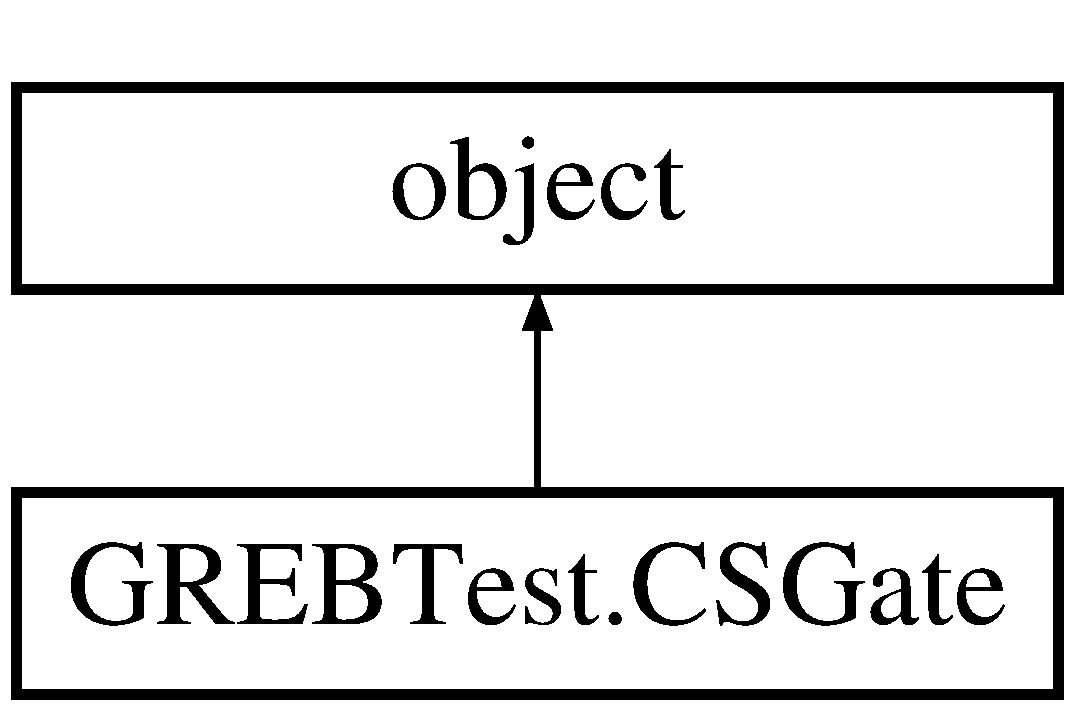
\includegraphics[height=2.000000cm]{class_g_r_e_b_test_1_1_c_s_gate}
\end{center}
\end{figure}
\subsection*{Public Member Functions}
\begin{DoxyCompactItemize}
\item 
def \hyperlink{class_g_r_e_b_test_1_1_c_s_gate_aaa67ea03a3a0f3c4e025c2f2fcf00547}{\+\_\+\+\_\+init\+\_\+\+\_\+} (self)
\begin{DoxyCompactList}\small\item\em Initialize minimum required variables for test list. \end{DoxyCompactList}\item 
def \hyperlink{class_g_r_e_b_test_1_1_c_s_gate_a4642819df1ae2fde9bf9fb14791b3d26}{run\+Test} (self)
\begin{DoxyCompactList}\small\item\em Run the test, save output to state variables. \end{DoxyCompactList}\item 
def \hyperlink{class_g_r_e_b_test_1_1_c_s_gate_afc9725472e61ad63c780ab0c186f14e4}{summarize} (self, summary)
\begin{DoxyCompactList}\small\item\em Summarize the test results for the cover page of the report. \end{DoxyCompactList}\item 
def \hyperlink{class_g_r_e_b_test_1_1_c_s_gate_a115b6c2e2446839ac38f180986fc9d41}{report} (self, pdf, report\+Path)
\begin{DoxyCompactList}\small\item\em generate this test\textquotesingle{}s page in the P\+DF report. \end{DoxyCompactList}\end{DoxyCompactItemize}


\subsection{Detailed Description}
Tests the current source gate. 



\subsection{Constructor \& Destructor Documentation}
\index{G\+R\+E\+B\+Test\+::\+C\+S\+Gate@{G\+R\+E\+B\+Test\+::\+C\+S\+Gate}!\+\_\+\+\_\+init\+\_\+\+\_\+@{\+\_\+\+\_\+init\+\_\+\+\_\+}}
\index{\+\_\+\+\_\+init\+\_\+\+\_\+@{\+\_\+\+\_\+init\+\_\+\+\_\+}!G\+R\+E\+B\+Test\+::\+C\+S\+Gate@{G\+R\+E\+B\+Test\+::\+C\+S\+Gate}}
\subsubsection[{\texorpdfstring{\+\_\+\+\_\+init\+\_\+\+\_\+(self)}{__init__(self)}}]{\setlength{\rightskip}{0pt plus 5cm}def G\+R\+E\+B\+Test.\+C\+S\+Gate.\+\_\+\+\_\+init\+\_\+\+\_\+ (
\begin{DoxyParamCaption}
\item[{}]{self}
\end{DoxyParamCaption}
)}\hypertarget{class_g_r_e_b_test_1_1_c_s_gate_aaa67ea03a3a0f3c4e025c2f2fcf00547}{}\label{class_g_r_e_b_test_1_1_c_s_gate_aaa67ea03a3a0f3c4e025c2f2fcf00547}


Initialize minimum required variables for test list. 



\subsection{Member Function Documentation}
\index{G\+R\+E\+B\+Test\+::\+C\+S\+Gate@{G\+R\+E\+B\+Test\+::\+C\+S\+Gate}!report@{report}}
\index{report@{report}!G\+R\+E\+B\+Test\+::\+C\+S\+Gate@{G\+R\+E\+B\+Test\+::\+C\+S\+Gate}}
\subsubsection[{\texorpdfstring{report(self, pdf, report\+Path)}{report(self, pdf, reportPath)}}]{\setlength{\rightskip}{0pt plus 5cm}def G\+R\+E\+B\+Test.\+C\+S\+Gate.\+report (
\begin{DoxyParamCaption}
\item[{}]{self, }
\item[{}]{pdf, }
\item[{}]{report\+Path}
\end{DoxyParamCaption}
)}\hypertarget{class_g_r_e_b_test_1_1_c_s_gate_a115b6c2e2446839ac38f180986fc9d41}{}\label{class_g_r_e_b_test_1_1_c_s_gate_a115b6c2e2446839ac38f180986fc9d41}


generate this test\textquotesingle{}s page in the P\+DF report. 


\begin{DoxyParams}{Parameters}
{\em pdf} & pyfpdf-\/compatible P\+DF object. \\
\hline
\end{DoxyParams}
\index{G\+R\+E\+B\+Test\+::\+C\+S\+Gate@{G\+R\+E\+B\+Test\+::\+C\+S\+Gate}!run\+Test@{run\+Test}}
\index{run\+Test@{run\+Test}!G\+R\+E\+B\+Test\+::\+C\+S\+Gate@{G\+R\+E\+B\+Test\+::\+C\+S\+Gate}}
\subsubsection[{\texorpdfstring{run\+Test(self)}{runTest(self)}}]{\setlength{\rightskip}{0pt plus 5cm}def G\+R\+E\+B\+Test.\+C\+S\+Gate.\+run\+Test (
\begin{DoxyParamCaption}
\item[{}]{self}
\end{DoxyParamCaption}
)}\hypertarget{class_g_r_e_b_test_1_1_c_s_gate_a4642819df1ae2fde9bf9fb14791b3d26}{}\label{class_g_r_e_b_test_1_1_c_s_gate_a4642819df1ae2fde9bf9fb14791b3d26}


Run the test, save output to state variables. 

\index{G\+R\+E\+B\+Test\+::\+C\+S\+Gate@{G\+R\+E\+B\+Test\+::\+C\+S\+Gate}!summarize@{summarize}}
\index{summarize@{summarize}!G\+R\+E\+B\+Test\+::\+C\+S\+Gate@{G\+R\+E\+B\+Test\+::\+C\+S\+Gate}}
\subsubsection[{\texorpdfstring{summarize(self, summary)}{summarize(self, summary)}}]{\setlength{\rightskip}{0pt plus 5cm}def G\+R\+E\+B\+Test.\+C\+S\+Gate.\+summarize (
\begin{DoxyParamCaption}
\item[{}]{self, }
\item[{}]{summary}
\end{DoxyParamCaption}
)}\hypertarget{class_g_r_e_b_test_1_1_c_s_gate_afc9725472e61ad63c780ab0c186f14e4}{}\label{class_g_r_e_b_test_1_1_c_s_gate_afc9725472e61ad63c780ab0c186f14e4}


Summarize the test results for the cover page of the report. 


\begin{DoxyParams}{Parameters}
{\em summary} & \hyperlink{class_g_r_e_b_test_1_1_summary}{Summary} obejct passed from Functional\+Test() \\
\hline
\end{DoxyParams}


The documentation for this class was generated from the following file\+:\begin{DoxyCompactItemize}
\item 
\hyperlink{_g_r_e_b_test_8py}{G\+R\+E\+B\+Test.\+py}\end{DoxyCompactItemize}

\hypertarget{class_w_r_e_b_test_1_1_functional_test}{}\section{W\+R\+E\+B\+Test.\+Functional\+Test Class Reference}
\label{class_w_r_e_b_test_1_1_functional_test}\index{W\+R\+E\+B\+Test.\+Functional\+Test@{W\+R\+E\+B\+Test.\+Functional\+Test}}


Runs the functional testing suite.  


Inheritance diagram for W\+R\+E\+B\+Test.\+Functional\+Test\+:\begin{figure}[H]
\begin{center}
\leavevmode
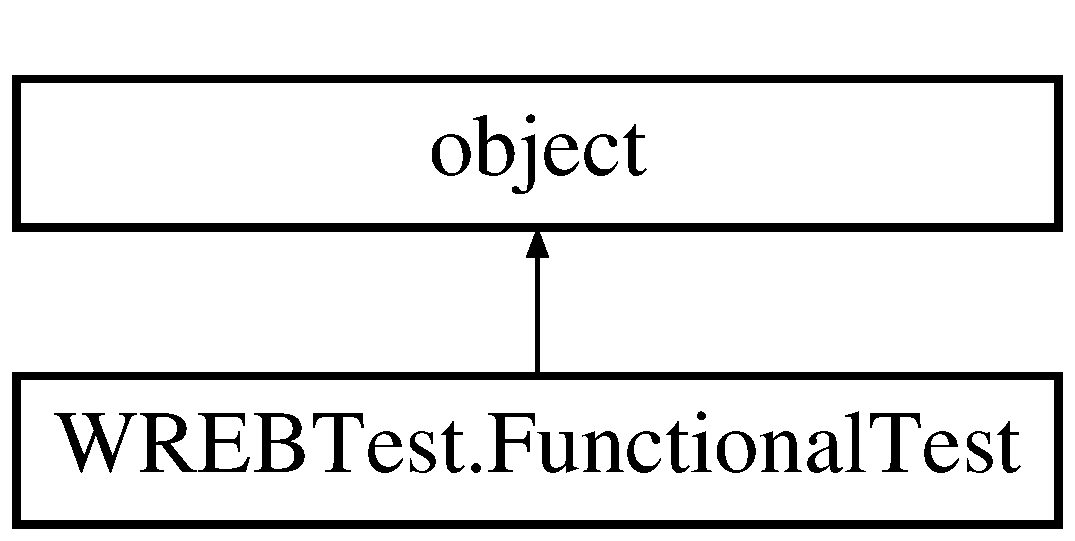
\includegraphics[height=2.000000cm]{class_w_r_e_b_test_1_1_functional_test}
\end{center}
\end{figure}
\subsection*{Public Member Functions}
\begin{DoxyCompactItemize}
\item 
def \hyperlink{class_w_r_e_b_test_1_1_functional_test_a18ce08cc79725a4b7b69e3859d19c849}{\+\_\+\+\_\+init\+\_\+\+\_\+} (self)
\begin{DoxyCompactList}\small\item\em Initializes the board information and list of tests to be run. \end{DoxyCompactList}\item 
def \hyperlink{class_w_r_e_b_test_1_1_functional_test_abc3fbd2a8e90988cb62731653df94cdf}{run\+Tests} (self)
\begin{DoxyCompactList}\small\item\em Run the tests. \end{DoxyCompactList}\item 
def \hyperlink{class_w_r_e_b_test_1_1_functional_test_a9b9f48ba6a45e7b47417bb3b39cfdaef}{generate\+Report} (self)
\begin{DoxyCompactList}\small\item\em Generate a pyfpdf-\/compatible P\+DF report from the test data. \end{DoxyCompactList}\end{DoxyCompactItemize}


\subsection{Detailed Description}
Runs the functional testing suite. 



\subsection{Constructor \& Destructor Documentation}
\index{W\+R\+E\+B\+Test\+::\+Functional\+Test@{W\+R\+E\+B\+Test\+::\+Functional\+Test}!\+\_\+\+\_\+init\+\_\+\+\_\+@{\+\_\+\+\_\+init\+\_\+\+\_\+}}
\index{\+\_\+\+\_\+init\+\_\+\+\_\+@{\+\_\+\+\_\+init\+\_\+\+\_\+}!W\+R\+E\+B\+Test\+::\+Functional\+Test@{W\+R\+E\+B\+Test\+::\+Functional\+Test}}
\subsubsection[{\texorpdfstring{\+\_\+\+\_\+init\+\_\+\+\_\+(self)}{__init__(self)}}]{\setlength{\rightskip}{0pt plus 5cm}def W\+R\+E\+B\+Test.\+Functional\+Test.\+\_\+\+\_\+init\+\_\+\+\_\+ (
\begin{DoxyParamCaption}
\item[{}]{self}
\end{DoxyParamCaption}
)}\hypertarget{class_w_r_e_b_test_1_1_functional_test_a18ce08cc79725a4b7b69e3859d19c849}{}\label{class_w_r_e_b_test_1_1_functional_test_a18ce08cc79725a4b7b69e3859d19c849}


Initializes the board information and list of tests to be run. 



\subsection{Member Function Documentation}
\index{W\+R\+E\+B\+Test\+::\+Functional\+Test@{W\+R\+E\+B\+Test\+::\+Functional\+Test}!generate\+Report@{generate\+Report}}
\index{generate\+Report@{generate\+Report}!W\+R\+E\+B\+Test\+::\+Functional\+Test@{W\+R\+E\+B\+Test\+::\+Functional\+Test}}
\subsubsection[{\texorpdfstring{generate\+Report(self)}{generateReport(self)}}]{\setlength{\rightskip}{0pt plus 5cm}def W\+R\+E\+B\+Test.\+Functional\+Test.\+generate\+Report (
\begin{DoxyParamCaption}
\item[{}]{self}
\end{DoxyParamCaption}
)}\hypertarget{class_w_r_e_b_test_1_1_functional_test_a9b9f48ba6a45e7b47417bb3b39cfdaef}{}\label{class_w_r_e_b_test_1_1_functional_test_a9b9f48ba6a45e7b47417bb3b39cfdaef}


Generate a pyfpdf-\/compatible P\+DF report from the test data. 

\index{W\+R\+E\+B\+Test\+::\+Functional\+Test@{W\+R\+E\+B\+Test\+::\+Functional\+Test}!run\+Tests@{run\+Tests}}
\index{run\+Tests@{run\+Tests}!W\+R\+E\+B\+Test\+::\+Functional\+Test@{W\+R\+E\+B\+Test\+::\+Functional\+Test}}
\subsubsection[{\texorpdfstring{run\+Tests(self)}{runTests(self)}}]{\setlength{\rightskip}{0pt plus 5cm}def W\+R\+E\+B\+Test.\+Functional\+Test.\+run\+Tests (
\begin{DoxyParamCaption}
\item[{}]{self}
\end{DoxyParamCaption}
)}\hypertarget{class_w_r_e_b_test_1_1_functional_test_abc3fbd2a8e90988cb62731653df94cdf}{}\label{class_w_r_e_b_test_1_1_functional_test_abc3fbd2a8e90988cb62731653df94cdf}


Run the tests. 



The documentation for this class was generated from the following file\+:\begin{DoxyCompactItemize}
\item 
\hyperlink{_w_r_e_b_test_8py}{W\+R\+E\+B\+Test.\+py}\end{DoxyCompactItemize}

\hypertarget{class_v_s_t_test_1_1_functional_test}{}\section{V\+S\+T\+Test.\+Functional\+Test Class Reference}
\label{class_v_s_t_test_1_1_functional_test}\index{V\+S\+T\+Test.\+Functional\+Test@{V\+S\+T\+Test.\+Functional\+Test}}


Runs the functional testing suite.  


Inheritance diagram for V\+S\+T\+Test.\+Functional\+Test\+:\begin{figure}[H]
\begin{center}
\leavevmode
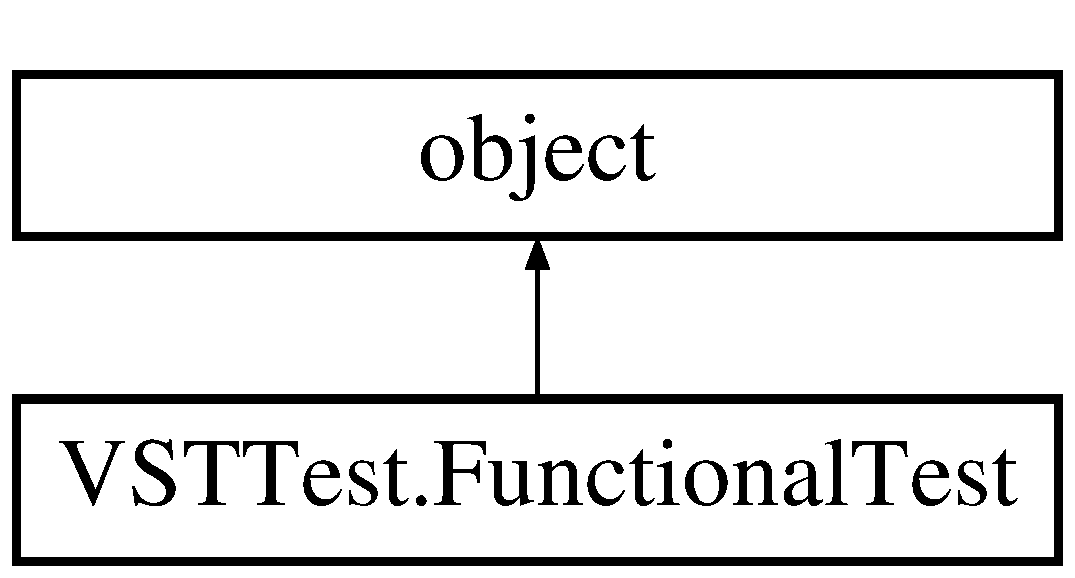
\includegraphics[height=2.000000cm]{class_v_s_t_test_1_1_functional_test}
\end{center}
\end{figure}
\subsection*{Public Member Functions}
\begin{DoxyCompactItemize}
\item 
def \hyperlink{class_v_s_t_test_1_1_functional_test_a8550a74691ecc31c808a274a8a16a76a}{run\+Tests} (self)
\begin{DoxyCompactList}\small\item\em Run the tests. \end{DoxyCompactList}\item 
def \hyperlink{class_v_s_t_test_1_1_functional_test_ac941fa6d87621ff6709715ea0b50dd49}{generate\+Report} (self)
\begin{DoxyCompactList}\small\item\em Generate a pyfpdf-\/compatible P\+DF report from the test data. \end{DoxyCompactList}\end{DoxyCompactItemize}


\subsection{Detailed Description}
Runs the functional testing suite. 

Tests are provided as a list of class initializations. 

\subsection{Member Function Documentation}
\index{V\+S\+T\+Test\+::\+Functional\+Test@{V\+S\+T\+Test\+::\+Functional\+Test}!generate\+Report@{generate\+Report}}
\index{generate\+Report@{generate\+Report}!V\+S\+T\+Test\+::\+Functional\+Test@{V\+S\+T\+Test\+::\+Functional\+Test}}
\subsubsection[{\texorpdfstring{generate\+Report(self)}{generateReport(self)}}]{\setlength{\rightskip}{0pt plus 5cm}def V\+S\+T\+Test.\+Functional\+Test.\+generate\+Report (
\begin{DoxyParamCaption}
\item[{}]{self}
\end{DoxyParamCaption}
)}\hypertarget{class_v_s_t_test_1_1_functional_test_ac941fa6d87621ff6709715ea0b50dd49}{}\label{class_v_s_t_test_1_1_functional_test_ac941fa6d87621ff6709715ea0b50dd49}


Generate a pyfpdf-\/compatible P\+DF report from the test data. 

\index{V\+S\+T\+Test\+::\+Functional\+Test@{V\+S\+T\+Test\+::\+Functional\+Test}!run\+Tests@{run\+Tests}}
\index{run\+Tests@{run\+Tests}!V\+S\+T\+Test\+::\+Functional\+Test@{V\+S\+T\+Test\+::\+Functional\+Test}}
\subsubsection[{\texorpdfstring{run\+Tests(self)}{runTests(self)}}]{\setlength{\rightskip}{0pt plus 5cm}def V\+S\+T\+Test.\+Functional\+Test.\+run\+Tests (
\begin{DoxyParamCaption}
\item[{}]{self}
\end{DoxyParamCaption}
)}\hypertarget{class_v_s_t_test_1_1_functional_test_a8550a74691ecc31c808a274a8a16a76a}{}\label{class_v_s_t_test_1_1_functional_test_a8550a74691ecc31c808a274a8a16a76a}


Run the tests. 



The documentation for this class was generated from the following file\+:\begin{DoxyCompactItemize}
\item 
\hyperlink{_v_s_t_test_8py}{V\+S\+T\+Test.\+py}\end{DoxyCompactItemize}

\hypertarget{class_g_r_e_b_test_1_1_functional_test}{}\section{G\+R\+E\+B\+Test.\+Functional\+Test Class Reference}
\label{class_g_r_e_b_test_1_1_functional_test}\index{G\+R\+E\+B\+Test.\+Functional\+Test@{G\+R\+E\+B\+Test.\+Functional\+Test}}


Runs the functional testing suite.  


Inheritance diagram for G\+R\+E\+B\+Test.\+Functional\+Test\+:\begin{figure}[H]
\begin{center}
\leavevmode
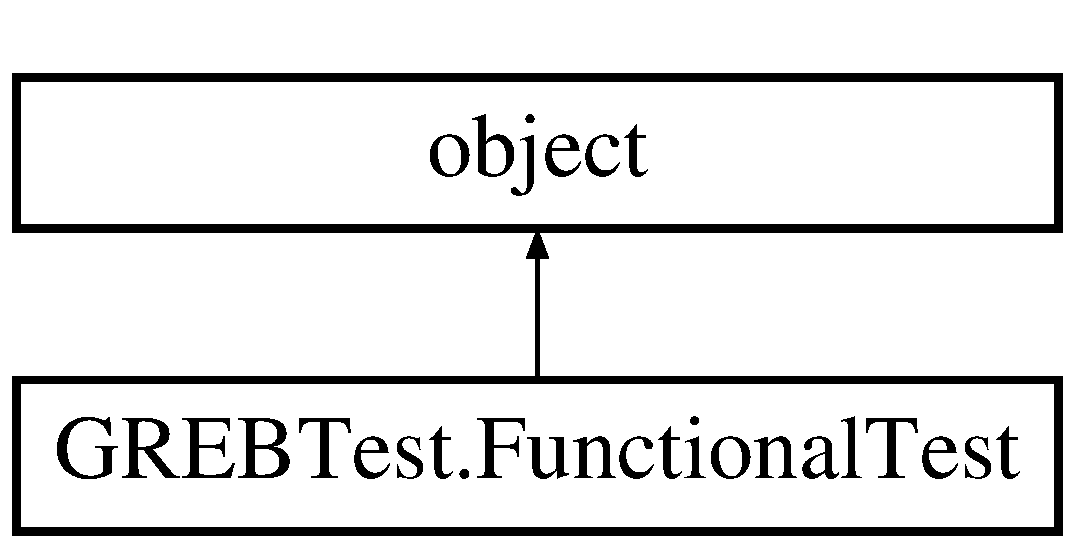
\includegraphics[height=2.000000cm]{class_g_r_e_b_test_1_1_functional_test}
\end{center}
\end{figure}
\subsection*{Public Member Functions}
\begin{DoxyCompactItemize}
\item 
def \hyperlink{class_g_r_e_b_test_1_1_functional_test_abc3c4c6a53cd099fde61418e5738acc9}{run\+Tests} (self)
\begin{DoxyCompactList}\small\item\em Run the tests. \end{DoxyCompactList}\item 
def \hyperlink{class_g_r_e_b_test_1_1_functional_test_ac0904992a4e2a98a5ec318bdc3656520}{generate\+Report} (self)
\begin{DoxyCompactList}\small\item\em Generate a pyfpdf-\/compatible P\+DF report from the test data. \end{DoxyCompactList}\end{DoxyCompactItemize}


\subsection{Detailed Description}
Runs the functional testing suite. 

Tests are provided as a list of class initializations. 

\subsection{Member Function Documentation}
\index{G\+R\+E\+B\+Test\+::\+Functional\+Test@{G\+R\+E\+B\+Test\+::\+Functional\+Test}!generate\+Report@{generate\+Report}}
\index{generate\+Report@{generate\+Report}!G\+R\+E\+B\+Test\+::\+Functional\+Test@{G\+R\+E\+B\+Test\+::\+Functional\+Test}}
\subsubsection[{\texorpdfstring{generate\+Report(self)}{generateReport(self)}}]{\setlength{\rightskip}{0pt plus 5cm}def G\+R\+E\+B\+Test.\+Functional\+Test.\+generate\+Report (
\begin{DoxyParamCaption}
\item[{}]{self}
\end{DoxyParamCaption}
)}\hypertarget{class_g_r_e_b_test_1_1_functional_test_ac0904992a4e2a98a5ec318bdc3656520}{}\label{class_g_r_e_b_test_1_1_functional_test_ac0904992a4e2a98a5ec318bdc3656520}


Generate a pyfpdf-\/compatible P\+DF report from the test data. 

\index{G\+R\+E\+B\+Test\+::\+Functional\+Test@{G\+R\+E\+B\+Test\+::\+Functional\+Test}!run\+Tests@{run\+Tests}}
\index{run\+Tests@{run\+Tests}!G\+R\+E\+B\+Test\+::\+Functional\+Test@{G\+R\+E\+B\+Test\+::\+Functional\+Test}}
\subsubsection[{\texorpdfstring{run\+Tests(self)}{runTests(self)}}]{\setlength{\rightskip}{0pt plus 5cm}def G\+R\+E\+B\+Test.\+Functional\+Test.\+run\+Tests (
\begin{DoxyParamCaption}
\item[{}]{self}
\end{DoxyParamCaption}
)}\hypertarget{class_g_r_e_b_test_1_1_functional_test_abc3c4c6a53cd099fde61418e5738acc9}{}\label{class_g_r_e_b_test_1_1_functional_test_abc3c4c6a53cd099fde61418e5738acc9}


Run the tests. 



The documentation for this class was generated from the following file\+:\begin{DoxyCompactItemize}
\item 
\hyperlink{_g_r_e_b_test_8py}{G\+R\+E\+B\+Test.\+py}\end{DoxyCompactItemize}

\hypertarget{class_v_s_t_test_1_1_g_d_bias}{}\section{V\+S\+T\+Test.\+G\+D\+Bias Class Reference}
\label{class_v_s_t_test_1_1_g_d_bias}\index{V\+S\+T\+Test.\+G\+D\+Bias@{V\+S\+T\+Test.\+G\+D\+Bias}}


Tests the guard drain performance.  


Inheritance diagram for V\+S\+T\+Test.\+G\+D\+Bias\+:\begin{figure}[H]
\begin{center}
\leavevmode
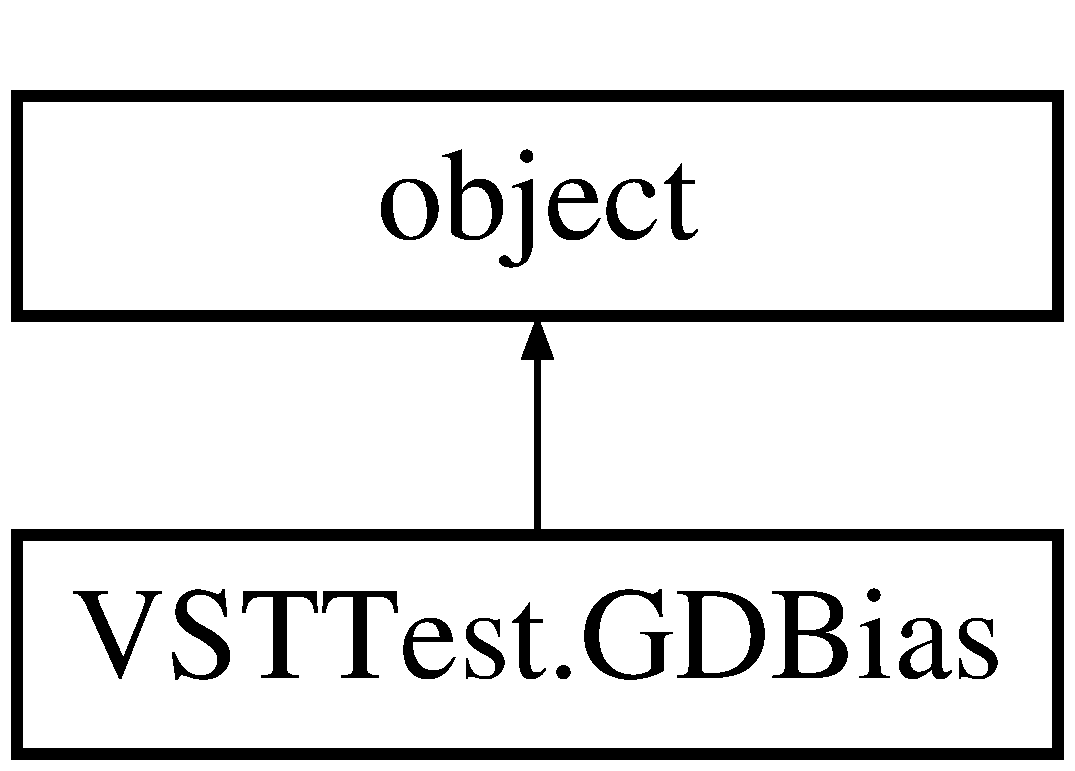
\includegraphics[height=2.000000cm]{class_v_s_t_test_1_1_g_d_bias}
\end{center}
\end{figure}
\subsection*{Public Member Functions}
\begin{DoxyCompactItemize}
\item 
def \hyperlink{class_v_s_t_test_1_1_g_d_bias_ae5f6661aa67e963b252893b33f7e48ed}{\+\_\+\+\_\+init\+\_\+\+\_\+} (self)
\begin{DoxyCompactList}\small\item\em Initialize minimum required variables for test list. \end{DoxyCompactList}\item 
def \hyperlink{class_v_s_t_test_1_1_g_d_bias_a7dab9741796cca9bc33aa0e28783a3f6}{run\+Test} (self)
\begin{DoxyCompactList}\small\item\em Run the test, save output to state variables. \end{DoxyCompactList}\item 
def \hyperlink{class_v_s_t_test_1_1_g_d_bias_a0a6175514ae3959b21b466d9e41e1976}{summarize} (self, summary)
\begin{DoxyCompactList}\small\item\em Summarize the test results for the cover page of the report. \end{DoxyCompactList}\item 
def \hyperlink{class_v_s_t_test_1_1_g_d_bias_ae2a38caef0c13f8e14a4e5157c7e257d}{report} (self, pdf, report\+Path)
\begin{DoxyCompactList}\small\item\em generate this test\textquotesingle{}s page in the P\+DF report. \end{DoxyCompactList}\end{DoxyCompactItemize}


\subsection{Detailed Description}
Tests the guard drain performance. 



\subsection{Constructor \& Destructor Documentation}
\index{V\+S\+T\+Test\+::\+G\+D\+Bias@{V\+S\+T\+Test\+::\+G\+D\+Bias}!\+\_\+\+\_\+init\+\_\+\+\_\+@{\+\_\+\+\_\+init\+\_\+\+\_\+}}
\index{\+\_\+\+\_\+init\+\_\+\+\_\+@{\+\_\+\+\_\+init\+\_\+\+\_\+}!V\+S\+T\+Test\+::\+G\+D\+Bias@{V\+S\+T\+Test\+::\+G\+D\+Bias}}
\subsubsection[{\texorpdfstring{\+\_\+\+\_\+init\+\_\+\+\_\+(self)}{__init__(self)}}]{\setlength{\rightskip}{0pt plus 5cm}def V\+S\+T\+Test.\+G\+D\+Bias.\+\_\+\+\_\+init\+\_\+\+\_\+ (
\begin{DoxyParamCaption}
\item[{}]{self}
\end{DoxyParamCaption}
)}\hypertarget{class_v_s_t_test_1_1_g_d_bias_ae5f6661aa67e963b252893b33f7e48ed}{}\label{class_v_s_t_test_1_1_g_d_bias_ae5f6661aa67e963b252893b33f7e48ed}


Initialize minimum required variables for test list. 



\subsection{Member Function Documentation}
\index{V\+S\+T\+Test\+::\+G\+D\+Bias@{V\+S\+T\+Test\+::\+G\+D\+Bias}!report@{report}}
\index{report@{report}!V\+S\+T\+Test\+::\+G\+D\+Bias@{V\+S\+T\+Test\+::\+G\+D\+Bias}}
\subsubsection[{\texorpdfstring{report(self, pdf, report\+Path)}{report(self, pdf, reportPath)}}]{\setlength{\rightskip}{0pt plus 5cm}def V\+S\+T\+Test.\+G\+D\+Bias.\+report (
\begin{DoxyParamCaption}
\item[{}]{self, }
\item[{}]{pdf, }
\item[{}]{report\+Path}
\end{DoxyParamCaption}
)}\hypertarget{class_v_s_t_test_1_1_g_d_bias_ae2a38caef0c13f8e14a4e5157c7e257d}{}\label{class_v_s_t_test_1_1_g_d_bias_ae2a38caef0c13f8e14a4e5157c7e257d}


generate this test\textquotesingle{}s page in the P\+DF report. 


\begin{DoxyParams}{Parameters}
{\em pdf} & pyfpdf-\/compatible P\+DF object. \\
\hline
{\em report\+Path} & Path of directory containing the pdf report \\
\hline
\end{DoxyParams}
\index{V\+S\+T\+Test\+::\+G\+D\+Bias@{V\+S\+T\+Test\+::\+G\+D\+Bias}!run\+Test@{run\+Test}}
\index{run\+Test@{run\+Test}!V\+S\+T\+Test\+::\+G\+D\+Bias@{V\+S\+T\+Test\+::\+G\+D\+Bias}}
\subsubsection[{\texorpdfstring{run\+Test(self)}{runTest(self)}}]{\setlength{\rightskip}{0pt plus 5cm}def V\+S\+T\+Test.\+G\+D\+Bias.\+run\+Test (
\begin{DoxyParamCaption}
\item[{}]{self}
\end{DoxyParamCaption}
)}\hypertarget{class_v_s_t_test_1_1_g_d_bias_a7dab9741796cca9bc33aa0e28783a3f6}{}\label{class_v_s_t_test_1_1_g_d_bias_a7dab9741796cca9bc33aa0e28783a3f6}


Run the test, save output to state variables. 

\index{V\+S\+T\+Test\+::\+G\+D\+Bias@{V\+S\+T\+Test\+::\+G\+D\+Bias}!summarize@{summarize}}
\index{summarize@{summarize}!V\+S\+T\+Test\+::\+G\+D\+Bias@{V\+S\+T\+Test\+::\+G\+D\+Bias}}
\subsubsection[{\texorpdfstring{summarize(self, summary)}{summarize(self, summary)}}]{\setlength{\rightskip}{0pt plus 5cm}def V\+S\+T\+Test.\+G\+D\+Bias.\+summarize (
\begin{DoxyParamCaption}
\item[{}]{self, }
\item[{}]{summary}
\end{DoxyParamCaption}
)}\hypertarget{class_v_s_t_test_1_1_g_d_bias_a0a6175514ae3959b21b466d9e41e1976}{}\label{class_v_s_t_test_1_1_g_d_bias_a0a6175514ae3959b21b466d9e41e1976}


Summarize the test results for the cover page of the report. 


\begin{DoxyParams}{Parameters}
{\em summary} & \hyperlink{class_v_s_t_test_1_1_summary}{Summary} obejct passed from Functional\+Test() \\
\hline
\end{DoxyParams}


The documentation for this class was generated from the following file\+:\begin{DoxyCompactItemize}
\item 
\hyperlink{_v_s_t_test_8py}{V\+S\+T\+Test.\+py}\end{DoxyCompactItemize}

\hypertarget{class_w_r_e_b_test_1_1_g_d_bias}{}\section{W\+R\+E\+B\+Test.\+G\+D\+Bias Class Reference}
\label{class_w_r_e_b_test_1_1_g_d_bias}\index{W\+R\+E\+B\+Test.\+G\+D\+Bias@{W\+R\+E\+B\+Test.\+G\+D\+Bias}}


Tests the guard drain performance.  


Inheritance diagram for W\+R\+E\+B\+Test.\+G\+D\+Bias\+:\begin{figure}[H]
\begin{center}
\leavevmode
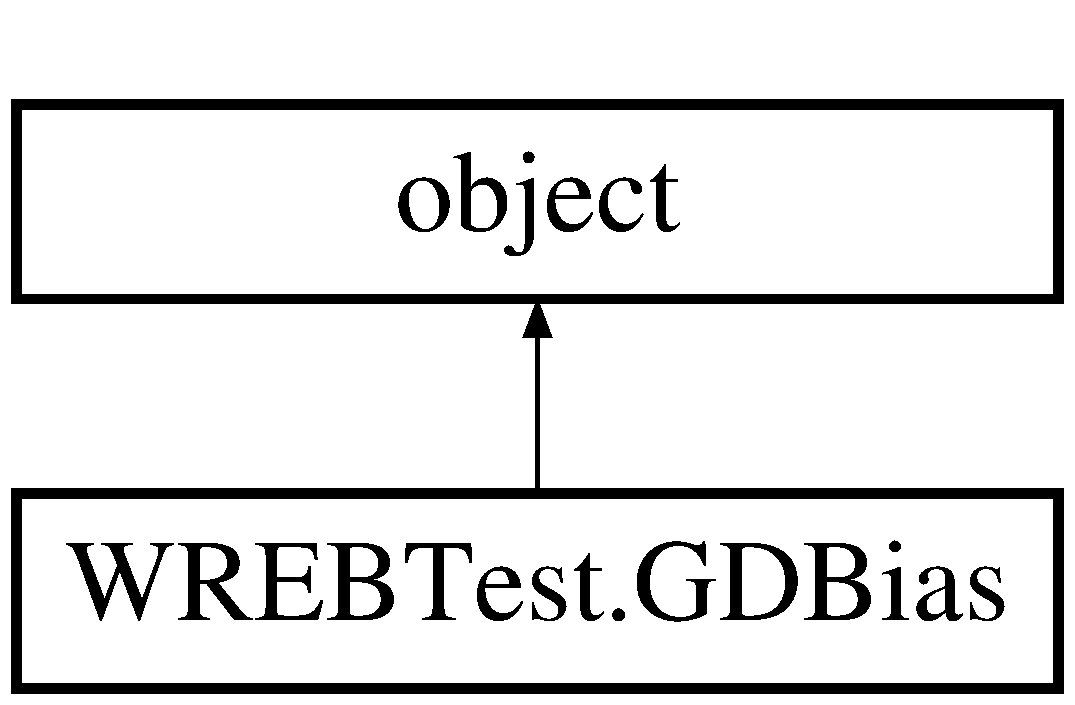
\includegraphics[height=2.000000cm]{class_w_r_e_b_test_1_1_g_d_bias}
\end{center}
\end{figure}
\subsection*{Public Member Functions}
\begin{DoxyCompactItemize}
\item 
def \hyperlink{class_w_r_e_b_test_1_1_g_d_bias_acf053e4e6e21e4a84814cfeb775f4c6b}{\+\_\+\+\_\+init\+\_\+\+\_\+} (self)
\begin{DoxyCompactList}\small\item\em Initialize minimum required variables for test list. \end{DoxyCompactList}\item 
def \hyperlink{class_w_r_e_b_test_1_1_g_d_bias_a994b19e58792f80591e2dc4dd4629bea}{run\+Test} (self)
\begin{DoxyCompactList}\small\item\em Run the test, save output to state variables. \end{DoxyCompactList}\item 
def \hyperlink{class_w_r_e_b_test_1_1_g_d_bias_a06f39560e8ecafd5299efd10e28dd7e9}{summarize} (self, summary)
\begin{DoxyCompactList}\small\item\em Summarize the test results for the cover page of the report. \end{DoxyCompactList}\item 
def \hyperlink{class_w_r_e_b_test_1_1_g_d_bias_a75fa14d7339831f013814bf1ca996f31}{report} (self, pdf)
\begin{DoxyCompactList}\small\item\em generate this test\textquotesingle{}s page in the P\+DF report. \end{DoxyCompactList}\end{DoxyCompactItemize}


\subsection{Detailed Description}
Tests the guard drain performance. 



\subsection{Constructor \& Destructor Documentation}
\index{W\+R\+E\+B\+Test\+::\+G\+D\+Bias@{W\+R\+E\+B\+Test\+::\+G\+D\+Bias}!\+\_\+\+\_\+init\+\_\+\+\_\+@{\+\_\+\+\_\+init\+\_\+\+\_\+}}
\index{\+\_\+\+\_\+init\+\_\+\+\_\+@{\+\_\+\+\_\+init\+\_\+\+\_\+}!W\+R\+E\+B\+Test\+::\+G\+D\+Bias@{W\+R\+E\+B\+Test\+::\+G\+D\+Bias}}
\subsubsection[{\texorpdfstring{\+\_\+\+\_\+init\+\_\+\+\_\+(self)}{__init__(self)}}]{\setlength{\rightskip}{0pt plus 5cm}def W\+R\+E\+B\+Test.\+G\+D\+Bias.\+\_\+\+\_\+init\+\_\+\+\_\+ (
\begin{DoxyParamCaption}
\item[{}]{self}
\end{DoxyParamCaption}
)}\hypertarget{class_w_r_e_b_test_1_1_g_d_bias_acf053e4e6e21e4a84814cfeb775f4c6b}{}\label{class_w_r_e_b_test_1_1_g_d_bias_acf053e4e6e21e4a84814cfeb775f4c6b}


Initialize minimum required variables for test list. 



\subsection{Member Function Documentation}
\index{W\+R\+E\+B\+Test\+::\+G\+D\+Bias@{W\+R\+E\+B\+Test\+::\+G\+D\+Bias}!report@{report}}
\index{report@{report}!W\+R\+E\+B\+Test\+::\+G\+D\+Bias@{W\+R\+E\+B\+Test\+::\+G\+D\+Bias}}
\subsubsection[{\texorpdfstring{report(self, pdf)}{report(self, pdf)}}]{\setlength{\rightskip}{0pt plus 5cm}def W\+R\+E\+B\+Test.\+G\+D\+Bias.\+report (
\begin{DoxyParamCaption}
\item[{}]{self, }
\item[{}]{pdf}
\end{DoxyParamCaption}
)}\hypertarget{class_w_r_e_b_test_1_1_g_d_bias_a75fa14d7339831f013814bf1ca996f31}{}\label{class_w_r_e_b_test_1_1_g_d_bias_a75fa14d7339831f013814bf1ca996f31}


generate this test\textquotesingle{}s page in the P\+DF report. 


\begin{DoxyParams}{Parameters}
{\em pdf} & pyfpdf-\/compatible P\+DF object. \\
\hline
\end{DoxyParams}
\index{W\+R\+E\+B\+Test\+::\+G\+D\+Bias@{W\+R\+E\+B\+Test\+::\+G\+D\+Bias}!run\+Test@{run\+Test}}
\index{run\+Test@{run\+Test}!W\+R\+E\+B\+Test\+::\+G\+D\+Bias@{W\+R\+E\+B\+Test\+::\+G\+D\+Bias}}
\subsubsection[{\texorpdfstring{run\+Test(self)}{runTest(self)}}]{\setlength{\rightskip}{0pt plus 5cm}def W\+R\+E\+B\+Test.\+G\+D\+Bias.\+run\+Test (
\begin{DoxyParamCaption}
\item[{}]{self}
\end{DoxyParamCaption}
)}\hypertarget{class_w_r_e_b_test_1_1_g_d_bias_a994b19e58792f80591e2dc4dd4629bea}{}\label{class_w_r_e_b_test_1_1_g_d_bias_a994b19e58792f80591e2dc4dd4629bea}


Run the test, save output to state variables. 

\index{W\+R\+E\+B\+Test\+::\+G\+D\+Bias@{W\+R\+E\+B\+Test\+::\+G\+D\+Bias}!summarize@{summarize}}
\index{summarize@{summarize}!W\+R\+E\+B\+Test\+::\+G\+D\+Bias@{W\+R\+E\+B\+Test\+::\+G\+D\+Bias}}
\subsubsection[{\texorpdfstring{summarize(self, summary)}{summarize(self, summary)}}]{\setlength{\rightskip}{0pt plus 5cm}def W\+R\+E\+B\+Test.\+G\+D\+Bias.\+summarize (
\begin{DoxyParamCaption}
\item[{}]{self, }
\item[{}]{summary}
\end{DoxyParamCaption}
)}\hypertarget{class_w_r_e_b_test_1_1_g_d_bias_a06f39560e8ecafd5299efd10e28dd7e9}{}\label{class_w_r_e_b_test_1_1_g_d_bias_a06f39560e8ecafd5299efd10e28dd7e9}


Summarize the test results for the cover page of the report. 


\begin{DoxyParams}{Parameters}
{\em summary} & \hyperlink{class_w_r_e_b_test_1_1_summary}{Summary} obejct passed from Functional\+Test() \\
\hline
\end{DoxyParams}


The documentation for this class was generated from the following file\+:\begin{DoxyCompactItemize}
\item 
\hyperlink{_w_r_e_b_test_8py}{W\+R\+E\+B\+Test.\+py}\end{DoxyCompactItemize}

\hypertarget{class_g_r_e_b_test_1_1_g_d_bias}{}\section{G\+R\+E\+B\+Test.\+G\+D\+Bias Class Reference}
\label{class_g_r_e_b_test_1_1_g_d_bias}\index{G\+R\+E\+B\+Test.\+G\+D\+Bias@{G\+R\+E\+B\+Test.\+G\+D\+Bias}}


Tests the guard drain performance.  


Inheritance diagram for G\+R\+E\+B\+Test.\+G\+D\+Bias\+:\begin{figure}[H]
\begin{center}
\leavevmode
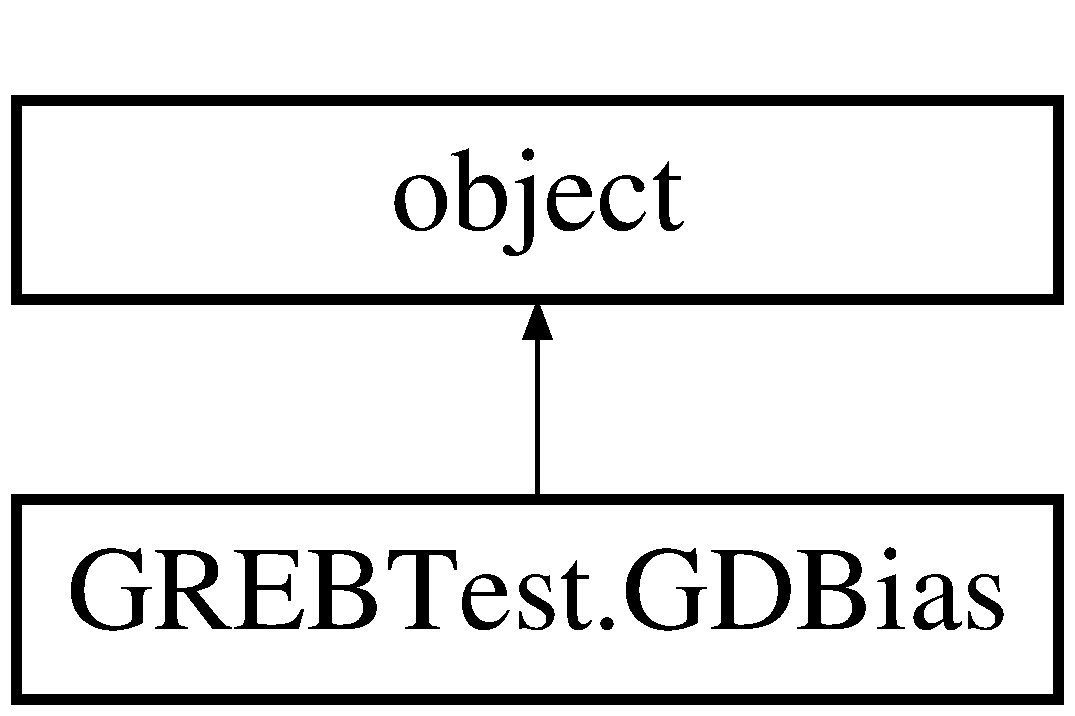
\includegraphics[height=2.000000cm]{class_g_r_e_b_test_1_1_g_d_bias}
\end{center}
\end{figure}
\subsection*{Public Member Functions}
\begin{DoxyCompactItemize}
\item 
def \hyperlink{class_g_r_e_b_test_1_1_g_d_bias_ac7f9e559681ac29efc4c27b3378cede2}{\+\_\+\+\_\+init\+\_\+\+\_\+} (self)
\begin{DoxyCompactList}\small\item\em Initialize minimum required variables for test list. \end{DoxyCompactList}\item 
def \hyperlink{class_g_r_e_b_test_1_1_g_d_bias_a321da21e9423c59f5b38fa3be84eac2a}{run\+Test} (self)
\begin{DoxyCompactList}\small\item\em Run the test, save output to state variables. \end{DoxyCompactList}\item 
def \hyperlink{class_g_r_e_b_test_1_1_g_d_bias_ae739a588383aa66af9452093d6e5b775}{summarize} (self, summary)
\begin{DoxyCompactList}\small\item\em Summarize the test results for the cover page of the report. \end{DoxyCompactList}\item 
def \hyperlink{class_g_r_e_b_test_1_1_g_d_bias_a46459b0db0d33a97664b1559046f2444}{report} (self, pdf, report\+Path)
\begin{DoxyCompactList}\small\item\em generate this test\textquotesingle{}s page in the P\+DF report. \end{DoxyCompactList}\end{DoxyCompactItemize}


\subsection{Detailed Description}
Tests the guard drain performance. 



\subsection{Constructor \& Destructor Documentation}
\index{G\+R\+E\+B\+Test\+::\+G\+D\+Bias@{G\+R\+E\+B\+Test\+::\+G\+D\+Bias}!\+\_\+\+\_\+init\+\_\+\+\_\+@{\+\_\+\+\_\+init\+\_\+\+\_\+}}
\index{\+\_\+\+\_\+init\+\_\+\+\_\+@{\+\_\+\+\_\+init\+\_\+\+\_\+}!G\+R\+E\+B\+Test\+::\+G\+D\+Bias@{G\+R\+E\+B\+Test\+::\+G\+D\+Bias}}
\subsubsection[{\texorpdfstring{\+\_\+\+\_\+init\+\_\+\+\_\+(self)}{__init__(self)}}]{\setlength{\rightskip}{0pt plus 5cm}def G\+R\+E\+B\+Test.\+G\+D\+Bias.\+\_\+\+\_\+init\+\_\+\+\_\+ (
\begin{DoxyParamCaption}
\item[{}]{self}
\end{DoxyParamCaption}
)}\hypertarget{class_g_r_e_b_test_1_1_g_d_bias_ac7f9e559681ac29efc4c27b3378cede2}{}\label{class_g_r_e_b_test_1_1_g_d_bias_ac7f9e559681ac29efc4c27b3378cede2}


Initialize minimum required variables for test list. 



\subsection{Member Function Documentation}
\index{G\+R\+E\+B\+Test\+::\+G\+D\+Bias@{G\+R\+E\+B\+Test\+::\+G\+D\+Bias}!report@{report}}
\index{report@{report}!G\+R\+E\+B\+Test\+::\+G\+D\+Bias@{G\+R\+E\+B\+Test\+::\+G\+D\+Bias}}
\subsubsection[{\texorpdfstring{report(self, pdf, report\+Path)}{report(self, pdf, reportPath)}}]{\setlength{\rightskip}{0pt plus 5cm}def G\+R\+E\+B\+Test.\+G\+D\+Bias.\+report (
\begin{DoxyParamCaption}
\item[{}]{self, }
\item[{}]{pdf, }
\item[{}]{report\+Path}
\end{DoxyParamCaption}
)}\hypertarget{class_g_r_e_b_test_1_1_g_d_bias_a46459b0db0d33a97664b1559046f2444}{}\label{class_g_r_e_b_test_1_1_g_d_bias_a46459b0db0d33a97664b1559046f2444}


generate this test\textquotesingle{}s page in the P\+DF report. 


\begin{DoxyParams}{Parameters}
{\em pdf} & pyfpdf-\/compatible P\+DF object. \\
\hline
{\em report\+Path} & Path of directory containing the pdf report \\
\hline
\end{DoxyParams}
\index{G\+R\+E\+B\+Test\+::\+G\+D\+Bias@{G\+R\+E\+B\+Test\+::\+G\+D\+Bias}!run\+Test@{run\+Test}}
\index{run\+Test@{run\+Test}!G\+R\+E\+B\+Test\+::\+G\+D\+Bias@{G\+R\+E\+B\+Test\+::\+G\+D\+Bias}}
\subsubsection[{\texorpdfstring{run\+Test(self)}{runTest(self)}}]{\setlength{\rightskip}{0pt plus 5cm}def G\+R\+E\+B\+Test.\+G\+D\+Bias.\+run\+Test (
\begin{DoxyParamCaption}
\item[{}]{self}
\end{DoxyParamCaption}
)}\hypertarget{class_g_r_e_b_test_1_1_g_d_bias_a321da21e9423c59f5b38fa3be84eac2a}{}\label{class_g_r_e_b_test_1_1_g_d_bias_a321da21e9423c59f5b38fa3be84eac2a}


Run the test, save output to state variables. 

\index{G\+R\+E\+B\+Test\+::\+G\+D\+Bias@{G\+R\+E\+B\+Test\+::\+G\+D\+Bias}!summarize@{summarize}}
\index{summarize@{summarize}!G\+R\+E\+B\+Test\+::\+G\+D\+Bias@{G\+R\+E\+B\+Test\+::\+G\+D\+Bias}}
\subsubsection[{\texorpdfstring{summarize(self, summary)}{summarize(self, summary)}}]{\setlength{\rightskip}{0pt plus 5cm}def G\+R\+E\+B\+Test.\+G\+D\+Bias.\+summarize (
\begin{DoxyParamCaption}
\item[{}]{self, }
\item[{}]{summary}
\end{DoxyParamCaption}
)}\hypertarget{class_g_r_e_b_test_1_1_g_d_bias_ae739a588383aa66af9452093d6e5b775}{}\label{class_g_r_e_b_test_1_1_g_d_bias_ae739a588383aa66af9452093d6e5b775}


Summarize the test results for the cover page of the report. 


\begin{DoxyParams}{Parameters}
{\em summary} & \hyperlink{class_g_r_e_b_test_1_1_summary}{Summary} obejct passed from Functional\+Test() \\
\hline
\end{DoxyParams}


The documentation for this class was generated from the following file\+:\begin{DoxyCompactItemize}
\item 
\hyperlink{_g_r_e_b_test_8py}{G\+R\+E\+B\+Test.\+py}\end{DoxyCompactItemize}

\hypertarget{class_w_r_e_b_test_1_1_g_u_i}{}\section{W\+R\+E\+B\+Test.\+G\+UI Class Reference}
\label{class_w_r_e_b_test_1_1_g_u_i}\index{W\+R\+E\+B\+Test.\+G\+UI@{W\+R\+E\+B\+Test.\+G\+UI}}


Dialog-\/based \hyperlink{class_w_r_e_b_test_1_1_g_u_i}{G\+UI} for displaying test progress and navigating options.  


Inheritance diagram for W\+R\+E\+B\+Test.\+G\+UI\+:\begin{figure}[H]
\begin{center}
\leavevmode
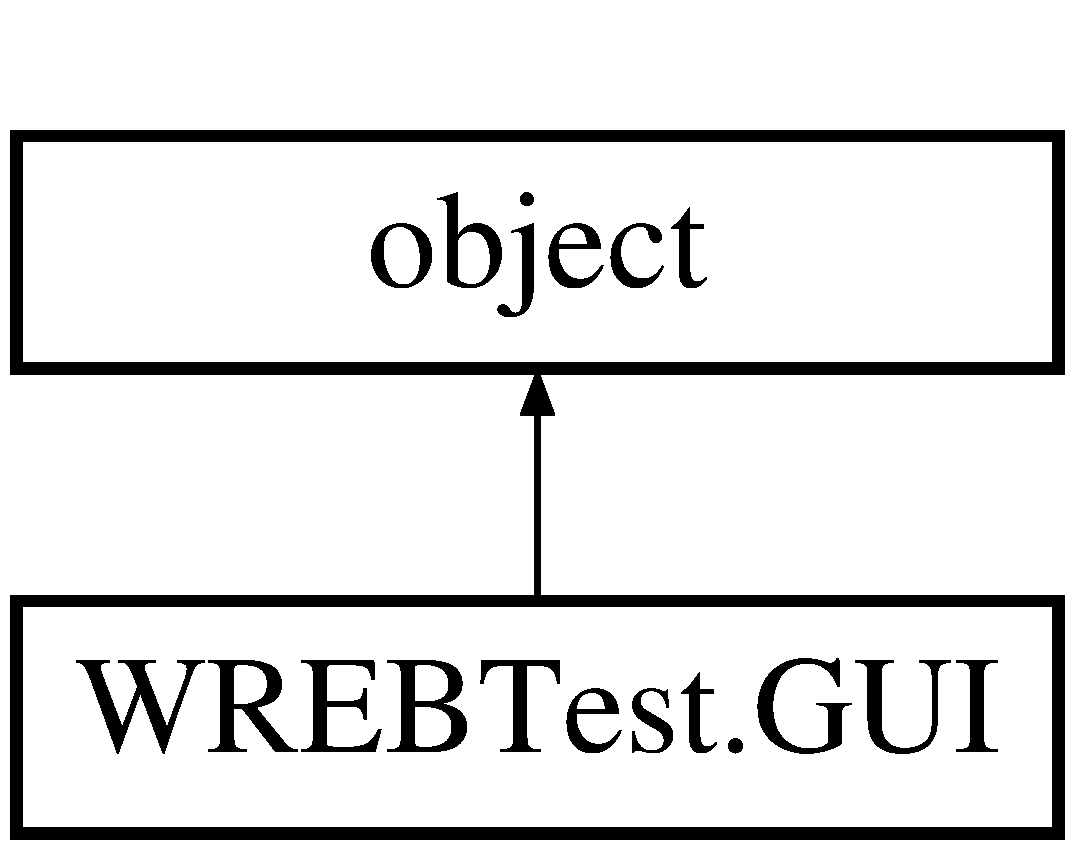
\includegraphics[height=2.000000cm]{class_w_r_e_b_test_1_1_g_u_i}
\end{center}
\end{figure}
\subsection*{Public Member Functions}
\begin{DoxyCompactItemize}
\item 
def \hyperlink{class_w_r_e_b_test_1_1_g_u_i_af16c984b23c92fbd1c31ef7e7f7528f6}{\+\_\+\+\_\+init\+\_\+\+\_\+} (self)
\begin{DoxyCompactList}\small\item\em Start the dialog. \end{DoxyCompactList}\item 
def \hyperlink{class_w_r_e_b_test_1_1_g_u_i_a6f9d70bcdf483cc55920068feacb8472}{update} (self, fn\+Test, generating\+P\+DF=False)
\begin{DoxyCompactList}\small\item\em Update the \hyperlink{class_w_r_e_b_test_1_1_g_u_i}{G\+UI} to display current testing progress. \end{DoxyCompactList}\item 
def \hyperlink{class_w_r_e_b_test_1_1_g_u_i_abf4a962a7a5b1da66157a96916bab756}{update\+Continuously} (self, fn\+Test)
\begin{DoxyCompactList}\small\item\em Continuously update the display every \+\_\+ seconds. \end{DoxyCompactList}\end{DoxyCompactItemize}


\subsection{Detailed Description}
Dialog-\/based \hyperlink{class_w_r_e_b_test_1_1_g_u_i}{G\+UI} for displaying test progress and navigating options. 



\subsection{Constructor \& Destructor Documentation}
\index{W\+R\+E\+B\+Test\+::\+G\+UI@{W\+R\+E\+B\+Test\+::\+G\+UI}!\+\_\+\+\_\+init\+\_\+\+\_\+@{\+\_\+\+\_\+init\+\_\+\+\_\+}}
\index{\+\_\+\+\_\+init\+\_\+\+\_\+@{\+\_\+\+\_\+init\+\_\+\+\_\+}!W\+R\+E\+B\+Test\+::\+G\+UI@{W\+R\+E\+B\+Test\+::\+G\+UI}}
\subsubsection[{\texorpdfstring{\+\_\+\+\_\+init\+\_\+\+\_\+(self)}{__init__(self)}}]{\setlength{\rightskip}{0pt plus 5cm}def W\+R\+E\+B\+Test.\+G\+U\+I.\+\_\+\+\_\+init\+\_\+\+\_\+ (
\begin{DoxyParamCaption}
\item[{}]{self}
\end{DoxyParamCaption}
)}\hypertarget{class_w_r_e_b_test_1_1_g_u_i_af16c984b23c92fbd1c31ef7e7f7528f6}{}\label{class_w_r_e_b_test_1_1_g_u_i_af16c984b23c92fbd1c31ef7e7f7528f6}


Start the dialog. 



\subsection{Member Function Documentation}
\index{W\+R\+E\+B\+Test\+::\+G\+UI@{W\+R\+E\+B\+Test\+::\+G\+UI}!update@{update}}
\index{update@{update}!W\+R\+E\+B\+Test\+::\+G\+UI@{W\+R\+E\+B\+Test\+::\+G\+UI}}
\subsubsection[{\texorpdfstring{update(self, fn\+Test, generating\+P\+D\+F=\+False)}{update(self, fnTest, generatingPDF=False)}}]{\setlength{\rightskip}{0pt plus 5cm}def W\+R\+E\+B\+Test.\+G\+U\+I.\+update (
\begin{DoxyParamCaption}
\item[{}]{self, }
\item[{}]{fn\+Test, }
\item[{}]{generating\+P\+DF = {\ttfamily False}}
\end{DoxyParamCaption}
)}\hypertarget{class_w_r_e_b_test_1_1_g_u_i_a6f9d70bcdf483cc55920068feacb8472}{}\label{class_w_r_e_b_test_1_1_g_u_i_a6f9d70bcdf483cc55920068feacb8472}


Update the \hyperlink{class_w_r_e_b_test_1_1_g_u_i}{G\+UI} to display current testing progress. 

\index{W\+R\+E\+B\+Test\+::\+G\+UI@{W\+R\+E\+B\+Test\+::\+G\+UI}!update\+Continuously@{update\+Continuously}}
\index{update\+Continuously@{update\+Continuously}!W\+R\+E\+B\+Test\+::\+G\+UI@{W\+R\+E\+B\+Test\+::\+G\+UI}}
\subsubsection[{\texorpdfstring{update\+Continuously(self, fn\+Test)}{updateContinuously(self, fnTest)}}]{\setlength{\rightskip}{0pt plus 5cm}def W\+R\+E\+B\+Test.\+G\+U\+I.\+update\+Continuously (
\begin{DoxyParamCaption}
\item[{}]{self, }
\item[{}]{fn\+Test}
\end{DoxyParamCaption}
)}\hypertarget{class_w_r_e_b_test_1_1_g_u_i_abf4a962a7a5b1da66157a96916bab756}{}\label{class_w_r_e_b_test_1_1_g_u_i_abf4a962a7a5b1da66157a96916bab756}


Continuously update the display every \+\_\+ seconds. 



The documentation for this class was generated from the following file\+:\begin{DoxyCompactItemize}
\item 
\hyperlink{_w_r_e_b_test_8py}{W\+R\+E\+B\+Test.\+py}\end{DoxyCompactItemize}

\hypertarget{class_v_s_t_test_1_1_g_u_i}{}\section{V\+S\+T\+Test.\+G\+UI Class Reference}
\label{class_v_s_t_test_1_1_g_u_i}\index{V\+S\+T\+Test.\+G\+UI@{V\+S\+T\+Test.\+G\+UI}}


Dialog-\/based \hyperlink{class_v_s_t_test_1_1_g_u_i}{G\+UI} for displaying test progress and navigating options.  


Inheritance diagram for V\+S\+T\+Test.\+G\+UI\+:\begin{figure}[H]
\begin{center}
\leavevmode
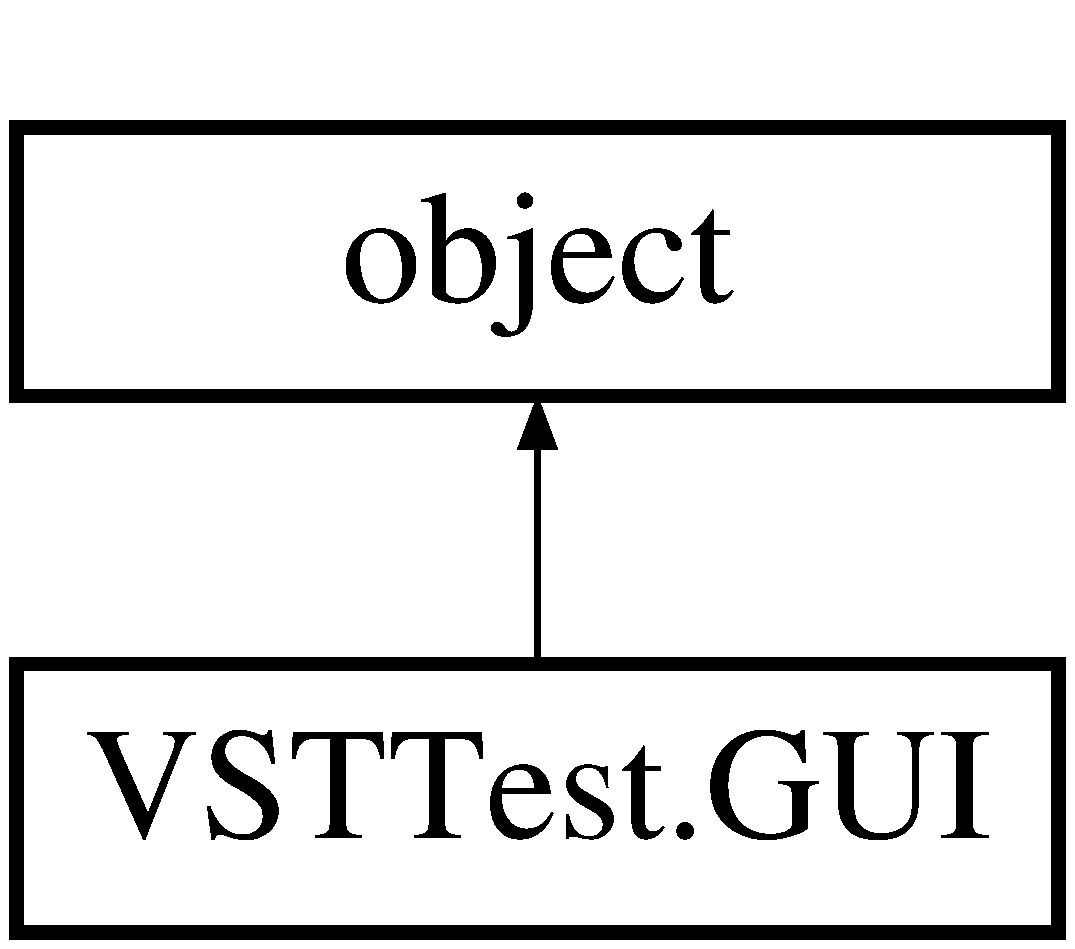
\includegraphics[height=2.000000cm]{class_v_s_t_test_1_1_g_u_i}
\end{center}
\end{figure}
\subsection*{Public Member Functions}
\begin{DoxyCompactItemize}
\item 
def \hyperlink{class_v_s_t_test_1_1_g_u_i_a51207db4115b235777b25bc15ba110d4}{\+\_\+\+\_\+init\+\_\+\+\_\+} (self)
\begin{DoxyCompactList}\small\item\em Start the dialog. \end{DoxyCompactList}\item 
def \hyperlink{class_v_s_t_test_1_1_g_u_i_a78e8fdaf0efd0c3b6fdc9c1b83ce9b58}{update} (self)
\begin{DoxyCompactList}\small\item\em Update the \hyperlink{class_v_s_t_test_1_1_g_u_i}{G\+UI} to display current testing progress. \end{DoxyCompactList}\item 
def \hyperlink{class_v_s_t_test_1_1_g_u_i_ae27c6cba235f7fb4c8c2f79f781dd143}{update\+Continuously} (self)
\begin{DoxyCompactList}\small\item\em Continuously update the display every \+\_\+ seconds. \end{DoxyCompactList}\item 
def \hyperlink{class_v_s_t_test_1_1_g_u_i_a740873dfe3a0d549b026f5534e2c301a}{start\+Update\+Continuously} (self)
\begin{DoxyCompactList}\small\item\em Start the self.\+update\+Continuously() procedure in a separate daemon thread. \end{DoxyCompactList}\item 
def \hyperlink{class_v_s_t_test_1_1_g_u_i_a38fec04bf02589c95708b329fdb04462}{start\+Menu} (self)
\begin{DoxyCompactList}\small\item\em Initial navigation menu. \end{DoxyCompactList}\item 
def \hyperlink{class_v_s_t_test_1_1_g_u_i_a4a5e04827eecb71faa569ce8c69774e6}{run\+Functional\+Test} (self)
\begin{DoxyCompactList}\small\item\em Runs the full suite of tests from the \hyperlink{class_v_s_t_test_1_1_g_u_i}{G\+UI}. \end{DoxyCompactList}\item 
def \hyperlink{class_v_s_t_test_1_1_g_u_i_a4db08c39bba6d63bdfdd7283f68a3cad}{run\+Custom\+Tests} (self)
\begin{DoxyCompactList}\small\item\em Allows the user to configure which tests should be run, and runs only those tests. \end{DoxyCompactList}\end{DoxyCompactItemize}


\subsection{Detailed Description}
Dialog-\/based \hyperlink{class_v_s_t_test_1_1_g_u_i}{G\+UI} for displaying test progress and navigating options. 



\subsection{Constructor \& Destructor Documentation}
\index{V\+S\+T\+Test\+::\+G\+UI@{V\+S\+T\+Test\+::\+G\+UI}!\+\_\+\+\_\+init\+\_\+\+\_\+@{\+\_\+\+\_\+init\+\_\+\+\_\+}}
\index{\+\_\+\+\_\+init\+\_\+\+\_\+@{\+\_\+\+\_\+init\+\_\+\+\_\+}!V\+S\+T\+Test\+::\+G\+UI@{V\+S\+T\+Test\+::\+G\+UI}}
\subsubsection[{\texorpdfstring{\+\_\+\+\_\+init\+\_\+\+\_\+(self)}{__init__(self)}}]{\setlength{\rightskip}{0pt plus 5cm}def V\+S\+T\+Test.\+G\+U\+I.\+\_\+\+\_\+init\+\_\+\+\_\+ (
\begin{DoxyParamCaption}
\item[{}]{self}
\end{DoxyParamCaption}
)}\hypertarget{class_v_s_t_test_1_1_g_u_i_a51207db4115b235777b25bc15ba110d4}{}\label{class_v_s_t_test_1_1_g_u_i_a51207db4115b235777b25bc15ba110d4}


Start the dialog. 



\subsection{Member Function Documentation}
\index{V\+S\+T\+Test\+::\+G\+UI@{V\+S\+T\+Test\+::\+G\+UI}!run\+Custom\+Tests@{run\+Custom\+Tests}}
\index{run\+Custom\+Tests@{run\+Custom\+Tests}!V\+S\+T\+Test\+::\+G\+UI@{V\+S\+T\+Test\+::\+G\+UI}}
\subsubsection[{\texorpdfstring{run\+Custom\+Tests(self)}{runCustomTests(self)}}]{\setlength{\rightskip}{0pt plus 5cm}def V\+S\+T\+Test.\+G\+U\+I.\+run\+Custom\+Tests (
\begin{DoxyParamCaption}
\item[{}]{self}
\end{DoxyParamCaption}
)}\hypertarget{class_v_s_t_test_1_1_g_u_i_a4db08c39bba6d63bdfdd7283f68a3cad}{}\label{class_v_s_t_test_1_1_g_u_i_a4db08c39bba6d63bdfdd7283f68a3cad}


Allows the user to configure which tests should be run, and runs only those tests. 

\index{V\+S\+T\+Test\+::\+G\+UI@{V\+S\+T\+Test\+::\+G\+UI}!run\+Functional\+Test@{run\+Functional\+Test}}
\index{run\+Functional\+Test@{run\+Functional\+Test}!V\+S\+T\+Test\+::\+G\+UI@{V\+S\+T\+Test\+::\+G\+UI}}
\subsubsection[{\texorpdfstring{run\+Functional\+Test(self)}{runFunctionalTest(self)}}]{\setlength{\rightskip}{0pt plus 5cm}def V\+S\+T\+Test.\+G\+U\+I.\+run\+Functional\+Test (
\begin{DoxyParamCaption}
\item[{}]{self}
\end{DoxyParamCaption}
)}\hypertarget{class_v_s_t_test_1_1_g_u_i_a4a5e04827eecb71faa569ce8c69774e6}{}\label{class_v_s_t_test_1_1_g_u_i_a4a5e04827eecb71faa569ce8c69774e6}


Runs the full suite of tests from the \hyperlink{class_v_s_t_test_1_1_g_u_i}{G\+UI}. 

\index{V\+S\+T\+Test\+::\+G\+UI@{V\+S\+T\+Test\+::\+G\+UI}!start\+Menu@{start\+Menu}}
\index{start\+Menu@{start\+Menu}!V\+S\+T\+Test\+::\+G\+UI@{V\+S\+T\+Test\+::\+G\+UI}}
\subsubsection[{\texorpdfstring{start\+Menu(self)}{startMenu(self)}}]{\setlength{\rightskip}{0pt plus 5cm}def V\+S\+T\+Test.\+G\+U\+I.\+start\+Menu (
\begin{DoxyParamCaption}
\item[{}]{self}
\end{DoxyParamCaption}
)}\hypertarget{class_v_s_t_test_1_1_g_u_i_a38fec04bf02589c95708b329fdb04462}{}\label{class_v_s_t_test_1_1_g_u_i_a38fec04bf02589c95708b329fdb04462}


Initial navigation menu. 

Checks that board is connected and presents the user with various options. \index{V\+S\+T\+Test\+::\+G\+UI@{V\+S\+T\+Test\+::\+G\+UI}!start\+Update\+Continuously@{start\+Update\+Continuously}}
\index{start\+Update\+Continuously@{start\+Update\+Continuously}!V\+S\+T\+Test\+::\+G\+UI@{V\+S\+T\+Test\+::\+G\+UI}}
\subsubsection[{\texorpdfstring{start\+Update\+Continuously(self)}{startUpdateContinuously(self)}}]{\setlength{\rightskip}{0pt plus 5cm}def V\+S\+T\+Test.\+G\+U\+I.\+start\+Update\+Continuously (
\begin{DoxyParamCaption}
\item[{}]{self}
\end{DoxyParamCaption}
)}\hypertarget{class_v_s_t_test_1_1_g_u_i_a740873dfe3a0d549b026f5534e2c301a}{}\label{class_v_s_t_test_1_1_g_u_i_a740873dfe3a0d549b026f5534e2c301a}


Start the self.\+update\+Continuously() procedure in a separate daemon thread. 

\index{V\+S\+T\+Test\+::\+G\+UI@{V\+S\+T\+Test\+::\+G\+UI}!update@{update}}
\index{update@{update}!V\+S\+T\+Test\+::\+G\+UI@{V\+S\+T\+Test\+::\+G\+UI}}
\subsubsection[{\texorpdfstring{update(self)}{update(self)}}]{\setlength{\rightskip}{0pt plus 5cm}def V\+S\+T\+Test.\+G\+U\+I.\+update (
\begin{DoxyParamCaption}
\item[{}]{self}
\end{DoxyParamCaption}
)}\hypertarget{class_v_s_t_test_1_1_g_u_i_a78e8fdaf0efd0c3b6fdc9c1b83ce9b58}{}\label{class_v_s_t_test_1_1_g_u_i_a78e8fdaf0efd0c3b6fdc9c1b83ce9b58}


Update the \hyperlink{class_v_s_t_test_1_1_g_u_i}{G\+UI} to display current testing progress. 

\index{V\+S\+T\+Test\+::\+G\+UI@{V\+S\+T\+Test\+::\+G\+UI}!update\+Continuously@{update\+Continuously}}
\index{update\+Continuously@{update\+Continuously}!V\+S\+T\+Test\+::\+G\+UI@{V\+S\+T\+Test\+::\+G\+UI}}
\subsubsection[{\texorpdfstring{update\+Continuously(self)}{updateContinuously(self)}}]{\setlength{\rightskip}{0pt plus 5cm}def V\+S\+T\+Test.\+G\+U\+I.\+update\+Continuously (
\begin{DoxyParamCaption}
\item[{}]{self}
\end{DoxyParamCaption}
)}\hypertarget{class_v_s_t_test_1_1_g_u_i_ae27c6cba235f7fb4c8c2f79f781dd143}{}\label{class_v_s_t_test_1_1_g_u_i_ae27c6cba235f7fb4c8c2f79f781dd143}


Continuously update the display every \+\_\+ seconds. 



The documentation for this class was generated from the following file\+:\begin{DoxyCompactItemize}
\item 
\hyperlink{_v_s_t_test_8py}{V\+S\+T\+Test.\+py}\end{DoxyCompactItemize}

\hypertarget{class_g_r_e_b_test_1_1_g_u_i}{}\section{G\+R\+E\+B\+Test.\+G\+UI Class Reference}
\label{class_g_r_e_b_test_1_1_g_u_i}\index{G\+R\+E\+B\+Test.\+G\+UI@{G\+R\+E\+B\+Test.\+G\+UI}}


Dialog-\/based \hyperlink{class_g_r_e_b_test_1_1_g_u_i}{G\+UI} for displaying test progress and navigating options.  


Inheritance diagram for G\+R\+E\+B\+Test.\+G\+UI\+:\begin{figure}[H]
\begin{center}
\leavevmode
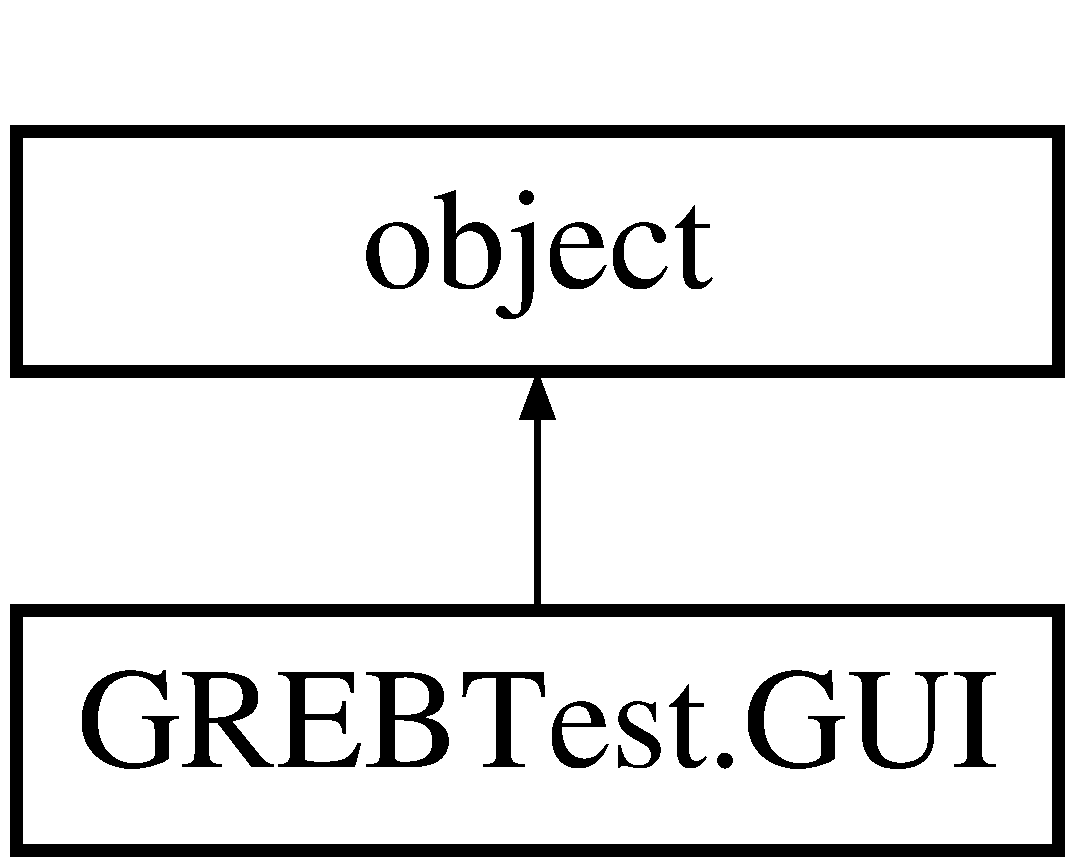
\includegraphics[height=2.000000cm]{class_g_r_e_b_test_1_1_g_u_i}
\end{center}
\end{figure}
\subsection*{Public Member Functions}
\begin{DoxyCompactItemize}
\item 
def \hyperlink{class_g_r_e_b_test_1_1_g_u_i_a4ecd31b36ad7f5c7bc2a42f0e32251b2}{\+\_\+\+\_\+init\+\_\+\+\_\+} (self)
\begin{DoxyCompactList}\small\item\em Start the dialog. \end{DoxyCompactList}\item 
def \hyperlink{class_g_r_e_b_test_1_1_g_u_i_a326df1d4b2efec002c02e7304066a2c3}{update} (self)
\begin{DoxyCompactList}\small\item\em Update the \hyperlink{class_g_r_e_b_test_1_1_g_u_i}{G\+UI} to display current testing progress. \end{DoxyCompactList}\item 
def \hyperlink{class_g_r_e_b_test_1_1_g_u_i_ae943e5f3a163d37991463b0a0a84d39a}{update\+Continuously} (self)
\begin{DoxyCompactList}\small\item\em Continuously update the display every \+\_\+ seconds. \end{DoxyCompactList}\item 
def \hyperlink{class_g_r_e_b_test_1_1_g_u_i_a8b1be69882cc710548d2fd7f7c05510c}{start\+Update\+Continuously} (self)
\begin{DoxyCompactList}\small\item\em Start the self.\+update\+Continuously() procedure in a separate daemon thread. \end{DoxyCompactList}\item 
def \hyperlink{class_g_r_e_b_test_1_1_g_u_i_a3bef1983e18d3cb039987a6b9d9d7ebe}{start\+Menu} (self)
\begin{DoxyCompactList}\small\item\em Initial navigation menu. \end{DoxyCompactList}\item 
def \hyperlink{class_g_r_e_b_test_1_1_g_u_i_a7bbbc241639e7c82f5bcc1bc9afef453}{run\+Functional\+Test} (self)
\begin{DoxyCompactList}\small\item\em Runs the full suite of tests from the \hyperlink{class_g_r_e_b_test_1_1_g_u_i}{G\+UI}. \end{DoxyCompactList}\item 
def \hyperlink{class_g_r_e_b_test_1_1_g_u_i_a13107c40c9106c861be757ad47a3052e}{run\+Custom\+Tests} (self)
\begin{DoxyCompactList}\small\item\em Allows the user to configure which tests should be run, and runs only those tests. \end{DoxyCompactList}\end{DoxyCompactItemize}


\subsection{Detailed Description}
Dialog-\/based \hyperlink{class_g_r_e_b_test_1_1_g_u_i}{G\+UI} for displaying test progress and navigating options. 



\subsection{Constructor \& Destructor Documentation}
\index{G\+R\+E\+B\+Test\+::\+G\+UI@{G\+R\+E\+B\+Test\+::\+G\+UI}!\+\_\+\+\_\+init\+\_\+\+\_\+@{\+\_\+\+\_\+init\+\_\+\+\_\+}}
\index{\+\_\+\+\_\+init\+\_\+\+\_\+@{\+\_\+\+\_\+init\+\_\+\+\_\+}!G\+R\+E\+B\+Test\+::\+G\+UI@{G\+R\+E\+B\+Test\+::\+G\+UI}}
\subsubsection[{\texorpdfstring{\+\_\+\+\_\+init\+\_\+\+\_\+(self)}{__init__(self)}}]{\setlength{\rightskip}{0pt plus 5cm}def G\+R\+E\+B\+Test.\+G\+U\+I.\+\_\+\+\_\+init\+\_\+\+\_\+ (
\begin{DoxyParamCaption}
\item[{}]{self}
\end{DoxyParamCaption}
)}\hypertarget{class_g_r_e_b_test_1_1_g_u_i_a4ecd31b36ad7f5c7bc2a42f0e32251b2}{}\label{class_g_r_e_b_test_1_1_g_u_i_a4ecd31b36ad7f5c7bc2a42f0e32251b2}


Start the dialog. 



\subsection{Member Function Documentation}
\index{G\+R\+E\+B\+Test\+::\+G\+UI@{G\+R\+E\+B\+Test\+::\+G\+UI}!run\+Custom\+Tests@{run\+Custom\+Tests}}
\index{run\+Custom\+Tests@{run\+Custom\+Tests}!G\+R\+E\+B\+Test\+::\+G\+UI@{G\+R\+E\+B\+Test\+::\+G\+UI}}
\subsubsection[{\texorpdfstring{run\+Custom\+Tests(self)}{runCustomTests(self)}}]{\setlength{\rightskip}{0pt plus 5cm}def G\+R\+E\+B\+Test.\+G\+U\+I.\+run\+Custom\+Tests (
\begin{DoxyParamCaption}
\item[{}]{self}
\end{DoxyParamCaption}
)}\hypertarget{class_g_r_e_b_test_1_1_g_u_i_a13107c40c9106c861be757ad47a3052e}{}\label{class_g_r_e_b_test_1_1_g_u_i_a13107c40c9106c861be757ad47a3052e}


Allows the user to configure which tests should be run, and runs only those tests. 

\index{G\+R\+E\+B\+Test\+::\+G\+UI@{G\+R\+E\+B\+Test\+::\+G\+UI}!run\+Functional\+Test@{run\+Functional\+Test}}
\index{run\+Functional\+Test@{run\+Functional\+Test}!G\+R\+E\+B\+Test\+::\+G\+UI@{G\+R\+E\+B\+Test\+::\+G\+UI}}
\subsubsection[{\texorpdfstring{run\+Functional\+Test(self)}{runFunctionalTest(self)}}]{\setlength{\rightskip}{0pt plus 5cm}def G\+R\+E\+B\+Test.\+G\+U\+I.\+run\+Functional\+Test (
\begin{DoxyParamCaption}
\item[{}]{self}
\end{DoxyParamCaption}
)}\hypertarget{class_g_r_e_b_test_1_1_g_u_i_a7bbbc241639e7c82f5bcc1bc9afef453}{}\label{class_g_r_e_b_test_1_1_g_u_i_a7bbbc241639e7c82f5bcc1bc9afef453}


Runs the full suite of tests from the \hyperlink{class_g_r_e_b_test_1_1_g_u_i}{G\+UI}. 

\index{G\+R\+E\+B\+Test\+::\+G\+UI@{G\+R\+E\+B\+Test\+::\+G\+UI}!start\+Menu@{start\+Menu}}
\index{start\+Menu@{start\+Menu}!G\+R\+E\+B\+Test\+::\+G\+UI@{G\+R\+E\+B\+Test\+::\+G\+UI}}
\subsubsection[{\texorpdfstring{start\+Menu(self)}{startMenu(self)}}]{\setlength{\rightskip}{0pt plus 5cm}def G\+R\+E\+B\+Test.\+G\+U\+I.\+start\+Menu (
\begin{DoxyParamCaption}
\item[{}]{self}
\end{DoxyParamCaption}
)}\hypertarget{class_g_r_e_b_test_1_1_g_u_i_a3bef1983e18d3cb039987a6b9d9d7ebe}{}\label{class_g_r_e_b_test_1_1_g_u_i_a3bef1983e18d3cb039987a6b9d9d7ebe}


Initial navigation menu. 

Checks that board is connected and presents the user with various options. \index{G\+R\+E\+B\+Test\+::\+G\+UI@{G\+R\+E\+B\+Test\+::\+G\+UI}!start\+Update\+Continuously@{start\+Update\+Continuously}}
\index{start\+Update\+Continuously@{start\+Update\+Continuously}!G\+R\+E\+B\+Test\+::\+G\+UI@{G\+R\+E\+B\+Test\+::\+G\+UI}}
\subsubsection[{\texorpdfstring{start\+Update\+Continuously(self)}{startUpdateContinuously(self)}}]{\setlength{\rightskip}{0pt plus 5cm}def G\+R\+E\+B\+Test.\+G\+U\+I.\+start\+Update\+Continuously (
\begin{DoxyParamCaption}
\item[{}]{self}
\end{DoxyParamCaption}
)}\hypertarget{class_g_r_e_b_test_1_1_g_u_i_a8b1be69882cc710548d2fd7f7c05510c}{}\label{class_g_r_e_b_test_1_1_g_u_i_a8b1be69882cc710548d2fd7f7c05510c}


Start the self.\+update\+Continuously() procedure in a separate daemon thread. 

\index{G\+R\+E\+B\+Test\+::\+G\+UI@{G\+R\+E\+B\+Test\+::\+G\+UI}!update@{update}}
\index{update@{update}!G\+R\+E\+B\+Test\+::\+G\+UI@{G\+R\+E\+B\+Test\+::\+G\+UI}}
\subsubsection[{\texorpdfstring{update(self)}{update(self)}}]{\setlength{\rightskip}{0pt plus 5cm}def G\+R\+E\+B\+Test.\+G\+U\+I.\+update (
\begin{DoxyParamCaption}
\item[{}]{self}
\end{DoxyParamCaption}
)}\hypertarget{class_g_r_e_b_test_1_1_g_u_i_a326df1d4b2efec002c02e7304066a2c3}{}\label{class_g_r_e_b_test_1_1_g_u_i_a326df1d4b2efec002c02e7304066a2c3}


Update the \hyperlink{class_g_r_e_b_test_1_1_g_u_i}{G\+UI} to display current testing progress. 

\index{G\+R\+E\+B\+Test\+::\+G\+UI@{G\+R\+E\+B\+Test\+::\+G\+UI}!update\+Continuously@{update\+Continuously}}
\index{update\+Continuously@{update\+Continuously}!G\+R\+E\+B\+Test\+::\+G\+UI@{G\+R\+E\+B\+Test\+::\+G\+UI}}
\subsubsection[{\texorpdfstring{update\+Continuously(self)}{updateContinuously(self)}}]{\setlength{\rightskip}{0pt plus 5cm}def G\+R\+E\+B\+Test.\+G\+U\+I.\+update\+Continuously (
\begin{DoxyParamCaption}
\item[{}]{self}
\end{DoxyParamCaption}
)}\hypertarget{class_g_r_e_b_test_1_1_g_u_i_ae943e5f3a163d37991463b0a0a84d39a}{}\label{class_g_r_e_b_test_1_1_g_u_i_ae943e5f3a163d37991463b0a0a84d39a}


Continuously update the display every \+\_\+ seconds. 



The documentation for this class was generated from the following file\+:\begin{DoxyCompactItemize}
\item 
\hyperlink{_g_r_e_b_test_8py}{G\+R\+E\+B\+Test.\+py}\end{DoxyCompactItemize}

\hypertarget{class_g_r_e_b_test_1_1_idle_current_consumption}{}\section{G\+R\+E\+B\+Test.\+Idle\+Current\+Consumption Class Reference}
\label{class_g_r_e_b_test_1_1_idle_current_consumption}\index{G\+R\+E\+B\+Test.\+Idle\+Current\+Consumption@{G\+R\+E\+B\+Test.\+Idle\+Current\+Consumption}}


Test for idle current consumption in the G\+R\+EB board.  


Inheritance diagram for G\+R\+E\+B\+Test.\+Idle\+Current\+Consumption\+:\begin{figure}[H]
\begin{center}
\leavevmode
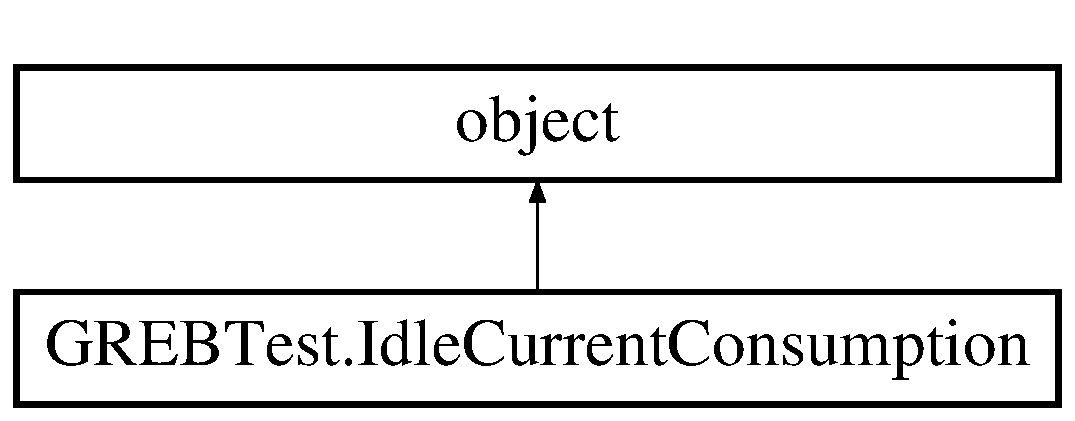
\includegraphics[height=2.000000cm]{class_g_r_e_b_test_1_1_idle_current_consumption}
\end{center}
\end{figure}
\subsection*{Public Member Functions}
\begin{DoxyCompactItemize}
\item 
def \hyperlink{class_g_r_e_b_test_1_1_idle_current_consumption_a69031fdeff95bec4109a9375b822693d}{\+\_\+\+\_\+init\+\_\+\+\_\+} (self)
\begin{DoxyCompactList}\small\item\em Initialize minimum required variables for test list. \end{DoxyCompactList}\item 
def \hyperlink{class_g_r_e_b_test_1_1_idle_current_consumption_a025d9d67ac6df090df0477c68b1dd8be}{run\+Test} (self)
\begin{DoxyCompactList}\small\item\em Run the test, save output to state variables. \end{DoxyCompactList}\item 
def \hyperlink{class_g_r_e_b_test_1_1_idle_current_consumption_a8f1c6ad70193d9795c5cb0a4d224a6ea}{summarize} (self, summary)
\begin{DoxyCompactList}\small\item\em Summarize the test results for the cover page of the report. \end{DoxyCompactList}\item 
def \hyperlink{class_g_r_e_b_test_1_1_idle_current_consumption_af0e85b6a116583cbc17294417d74b6ce}{report} (self, pdf, report\+Path)
\begin{DoxyCompactList}\small\item\em generate this test\textquotesingle{}s page in the P\+DF report. \end{DoxyCompactList}\end{DoxyCompactItemize}


\subsection{Detailed Description}
Test for idle current consumption in the G\+R\+EB board. 



\subsection{Constructor \& Destructor Documentation}
\index{G\+R\+E\+B\+Test\+::\+Idle\+Current\+Consumption@{G\+R\+E\+B\+Test\+::\+Idle\+Current\+Consumption}!\+\_\+\+\_\+init\+\_\+\+\_\+@{\+\_\+\+\_\+init\+\_\+\+\_\+}}
\index{\+\_\+\+\_\+init\+\_\+\+\_\+@{\+\_\+\+\_\+init\+\_\+\+\_\+}!G\+R\+E\+B\+Test\+::\+Idle\+Current\+Consumption@{G\+R\+E\+B\+Test\+::\+Idle\+Current\+Consumption}}
\subsubsection[{\texorpdfstring{\+\_\+\+\_\+init\+\_\+\+\_\+(self)}{__init__(self)}}]{\setlength{\rightskip}{0pt plus 5cm}def G\+R\+E\+B\+Test.\+Idle\+Current\+Consumption.\+\_\+\+\_\+init\+\_\+\+\_\+ (
\begin{DoxyParamCaption}
\item[{}]{self}
\end{DoxyParamCaption}
)}\hypertarget{class_g_r_e_b_test_1_1_idle_current_consumption_a69031fdeff95bec4109a9375b822693d}{}\label{class_g_r_e_b_test_1_1_idle_current_consumption_a69031fdeff95bec4109a9375b822693d}


Initialize minimum required variables for test list. 



\subsection{Member Function Documentation}
\index{G\+R\+E\+B\+Test\+::\+Idle\+Current\+Consumption@{G\+R\+E\+B\+Test\+::\+Idle\+Current\+Consumption}!report@{report}}
\index{report@{report}!G\+R\+E\+B\+Test\+::\+Idle\+Current\+Consumption@{G\+R\+E\+B\+Test\+::\+Idle\+Current\+Consumption}}
\subsubsection[{\texorpdfstring{report(self, pdf, report\+Path)}{report(self, pdf, reportPath)}}]{\setlength{\rightskip}{0pt plus 5cm}def G\+R\+E\+B\+Test.\+Idle\+Current\+Consumption.\+report (
\begin{DoxyParamCaption}
\item[{}]{self, }
\item[{}]{pdf, }
\item[{}]{report\+Path}
\end{DoxyParamCaption}
)}\hypertarget{class_g_r_e_b_test_1_1_idle_current_consumption_af0e85b6a116583cbc17294417d74b6ce}{}\label{class_g_r_e_b_test_1_1_idle_current_consumption_af0e85b6a116583cbc17294417d74b6ce}


generate this test\textquotesingle{}s page in the P\+DF report. 


\begin{DoxyParams}{Parameters}
{\em pdf} & pyfpdf-\/compatible P\+DF object. \\
\hline
{\em report\+Path} & Path of directory containing the pdf report \\
\hline
\end{DoxyParams}
\index{G\+R\+E\+B\+Test\+::\+Idle\+Current\+Consumption@{G\+R\+E\+B\+Test\+::\+Idle\+Current\+Consumption}!run\+Test@{run\+Test}}
\index{run\+Test@{run\+Test}!G\+R\+E\+B\+Test\+::\+Idle\+Current\+Consumption@{G\+R\+E\+B\+Test\+::\+Idle\+Current\+Consumption}}
\subsubsection[{\texorpdfstring{run\+Test(self)}{runTest(self)}}]{\setlength{\rightskip}{0pt plus 5cm}def G\+R\+E\+B\+Test.\+Idle\+Current\+Consumption.\+run\+Test (
\begin{DoxyParamCaption}
\item[{}]{self}
\end{DoxyParamCaption}
)}\hypertarget{class_g_r_e_b_test_1_1_idle_current_consumption_a025d9d67ac6df090df0477c68b1dd8be}{}\label{class_g_r_e_b_test_1_1_idle_current_consumption_a025d9d67ac6df090df0477c68b1dd8be}


Run the test, save output to state variables. 

\index{G\+R\+E\+B\+Test\+::\+Idle\+Current\+Consumption@{G\+R\+E\+B\+Test\+::\+Idle\+Current\+Consumption}!summarize@{summarize}}
\index{summarize@{summarize}!G\+R\+E\+B\+Test\+::\+Idle\+Current\+Consumption@{G\+R\+E\+B\+Test\+::\+Idle\+Current\+Consumption}}
\subsubsection[{\texorpdfstring{summarize(self, summary)}{summarize(self, summary)}}]{\setlength{\rightskip}{0pt plus 5cm}def G\+R\+E\+B\+Test.\+Idle\+Current\+Consumption.\+summarize (
\begin{DoxyParamCaption}
\item[{}]{self, }
\item[{}]{summary}
\end{DoxyParamCaption}
)}\hypertarget{class_g_r_e_b_test_1_1_idle_current_consumption_a8f1c6ad70193d9795c5cb0a4d224a6ea}{}\label{class_g_r_e_b_test_1_1_idle_current_consumption_a8f1c6ad70193d9795c5cb0a4d224a6ea}


Summarize the test results for the cover page of the report. 


\begin{DoxyParams}{Parameters}
{\em summary} & \hyperlink{class_g_r_e_b_test_1_1_summary}{Summary} obejct passed from Functional\+Test() \\
\hline
\end{DoxyParams}


The documentation for this class was generated from the following file\+:\begin{DoxyCompactItemize}
\item 
\hyperlink{_g_r_e_b_test_8py}{G\+R\+E\+B\+Test.\+py}\end{DoxyCompactItemize}

\hypertarget{class_w_r_e_b_test_1_1_idle_current_consumption}{}\section{W\+R\+E\+B\+Test.\+Idle\+Current\+Consumption Class Reference}
\label{class_w_r_e_b_test_1_1_idle_current_consumption}\index{W\+R\+E\+B\+Test.\+Idle\+Current\+Consumption@{W\+R\+E\+B\+Test.\+Idle\+Current\+Consumption}}


Test for idle current consumption in the W\+R\+EB board.  


Inheritance diagram for W\+R\+E\+B\+Test.\+Idle\+Current\+Consumption\+:\begin{figure}[H]
\begin{center}
\leavevmode
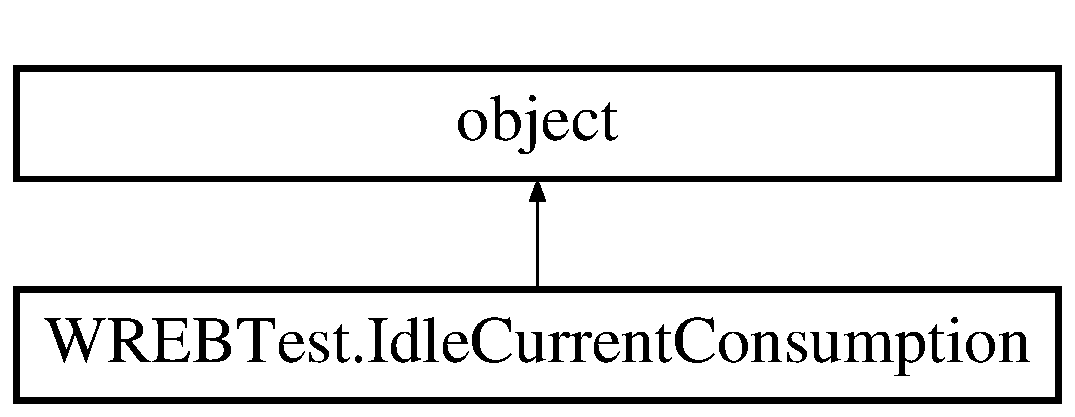
\includegraphics[height=2.000000cm]{class_w_r_e_b_test_1_1_idle_current_consumption}
\end{center}
\end{figure}
\subsection*{Public Member Functions}
\begin{DoxyCompactItemize}
\item 
def \hyperlink{class_w_r_e_b_test_1_1_idle_current_consumption_a7aec47c458783e4d1cdfe0df5c4973e3}{\+\_\+\+\_\+init\+\_\+\+\_\+} (self)
\begin{DoxyCompactList}\small\item\em Initialize minimum required variables for test list. \end{DoxyCompactList}\item 
def \hyperlink{class_w_r_e_b_test_1_1_idle_current_consumption_aeaa52c734d7528a4c120939189e4a500}{run\+Test} (self)
\begin{DoxyCompactList}\small\item\em Run the test, save output to state variables. \end{DoxyCompactList}\item 
def \hyperlink{class_w_r_e_b_test_1_1_idle_current_consumption_a867a45d43d305dcb08d1db2560c8db33}{summarize} (self, summary)
\begin{DoxyCompactList}\small\item\em Summarize the test results for the cover page of the report. \end{DoxyCompactList}\item 
def \hyperlink{class_w_r_e_b_test_1_1_idle_current_consumption_acb8e46859a43b20689ca8f30ea05e5a6}{report} (self, pdf, report\+Path)
\begin{DoxyCompactList}\small\item\em generate this test\textquotesingle{}s page in the P\+DF report. \end{DoxyCompactList}\end{DoxyCompactItemize}


\subsection{Detailed Description}
Test for idle current consumption in the W\+R\+EB board. 



\subsection{Constructor \& Destructor Documentation}
\index{W\+R\+E\+B\+Test\+::\+Idle\+Current\+Consumption@{W\+R\+E\+B\+Test\+::\+Idle\+Current\+Consumption}!\+\_\+\+\_\+init\+\_\+\+\_\+@{\+\_\+\+\_\+init\+\_\+\+\_\+}}
\index{\+\_\+\+\_\+init\+\_\+\+\_\+@{\+\_\+\+\_\+init\+\_\+\+\_\+}!W\+R\+E\+B\+Test\+::\+Idle\+Current\+Consumption@{W\+R\+E\+B\+Test\+::\+Idle\+Current\+Consumption}}
\subsubsection[{\texorpdfstring{\+\_\+\+\_\+init\+\_\+\+\_\+(self)}{__init__(self)}}]{\setlength{\rightskip}{0pt plus 5cm}def W\+R\+E\+B\+Test.\+Idle\+Current\+Consumption.\+\_\+\+\_\+init\+\_\+\+\_\+ (
\begin{DoxyParamCaption}
\item[{}]{self}
\end{DoxyParamCaption}
)}\hypertarget{class_w_r_e_b_test_1_1_idle_current_consumption_a7aec47c458783e4d1cdfe0df5c4973e3}{}\label{class_w_r_e_b_test_1_1_idle_current_consumption_a7aec47c458783e4d1cdfe0df5c4973e3}


Initialize minimum required variables for test list. 



\subsection{Member Function Documentation}
\index{W\+R\+E\+B\+Test\+::\+Idle\+Current\+Consumption@{W\+R\+E\+B\+Test\+::\+Idle\+Current\+Consumption}!report@{report}}
\index{report@{report}!W\+R\+E\+B\+Test\+::\+Idle\+Current\+Consumption@{W\+R\+E\+B\+Test\+::\+Idle\+Current\+Consumption}}
\subsubsection[{\texorpdfstring{report(self, pdf, report\+Path)}{report(self, pdf, reportPath)}}]{\setlength{\rightskip}{0pt plus 5cm}def W\+R\+E\+B\+Test.\+Idle\+Current\+Consumption.\+report (
\begin{DoxyParamCaption}
\item[{}]{self, }
\item[{}]{pdf, }
\item[{}]{report\+Path}
\end{DoxyParamCaption}
)}\hypertarget{class_w_r_e_b_test_1_1_idle_current_consumption_acb8e46859a43b20689ca8f30ea05e5a6}{}\label{class_w_r_e_b_test_1_1_idle_current_consumption_acb8e46859a43b20689ca8f30ea05e5a6}


generate this test\textquotesingle{}s page in the P\+DF report. 


\begin{DoxyParams}{Parameters}
{\em pdf} & pyfpdf-\/compatible P\+DF object. \\
\hline
{\em report\+Path} & Path of directory containing the pdf report \\
\hline
\end{DoxyParams}
\index{W\+R\+E\+B\+Test\+::\+Idle\+Current\+Consumption@{W\+R\+E\+B\+Test\+::\+Idle\+Current\+Consumption}!run\+Test@{run\+Test}}
\index{run\+Test@{run\+Test}!W\+R\+E\+B\+Test\+::\+Idle\+Current\+Consumption@{W\+R\+E\+B\+Test\+::\+Idle\+Current\+Consumption}}
\subsubsection[{\texorpdfstring{run\+Test(self)}{runTest(self)}}]{\setlength{\rightskip}{0pt plus 5cm}def W\+R\+E\+B\+Test.\+Idle\+Current\+Consumption.\+run\+Test (
\begin{DoxyParamCaption}
\item[{}]{self}
\end{DoxyParamCaption}
)}\hypertarget{class_w_r_e_b_test_1_1_idle_current_consumption_aeaa52c734d7528a4c120939189e4a500}{}\label{class_w_r_e_b_test_1_1_idle_current_consumption_aeaa52c734d7528a4c120939189e4a500}


Run the test, save output to state variables. 

\index{W\+R\+E\+B\+Test\+::\+Idle\+Current\+Consumption@{W\+R\+E\+B\+Test\+::\+Idle\+Current\+Consumption}!summarize@{summarize}}
\index{summarize@{summarize}!W\+R\+E\+B\+Test\+::\+Idle\+Current\+Consumption@{W\+R\+E\+B\+Test\+::\+Idle\+Current\+Consumption}}
\subsubsection[{\texorpdfstring{summarize(self, summary)}{summarize(self, summary)}}]{\setlength{\rightskip}{0pt plus 5cm}def W\+R\+E\+B\+Test.\+Idle\+Current\+Consumption.\+summarize (
\begin{DoxyParamCaption}
\item[{}]{self, }
\item[{}]{summary}
\end{DoxyParamCaption}
)}\hypertarget{class_w_r_e_b_test_1_1_idle_current_consumption_a867a45d43d305dcb08d1db2560c8db33}{}\label{class_w_r_e_b_test_1_1_idle_current_consumption_a867a45d43d305dcb08d1db2560c8db33}


Summarize the test results for the cover page of the report. 


\begin{DoxyParams}{Parameters}
{\em summary} & \hyperlink{class_w_r_e_b_test_1_1_summary}{Summary} obejct passed from Functional\+Test() \\
\hline
\end{DoxyParams}


The documentation for this class was generated from the following file\+:\begin{DoxyCompactItemize}
\item 
\hyperlink{_w_r_e_b_test_8py}{W\+R\+E\+B\+Test.\+py}\end{DoxyCompactItemize}

\hypertarget{class_v_s_t_test_1_1_idle_current_consumption}{}\section{V\+S\+T\+Test.\+Idle\+Current\+Consumption Class Reference}
\label{class_v_s_t_test_1_1_idle_current_consumption}\index{V\+S\+T\+Test.\+Idle\+Current\+Consumption@{V\+S\+T\+Test.\+Idle\+Current\+Consumption}}


Test for idle current consumption in the V\+ST board.  


Inheritance diagram for V\+S\+T\+Test.\+Idle\+Current\+Consumption\+:\begin{figure}[H]
\begin{center}
\leavevmode
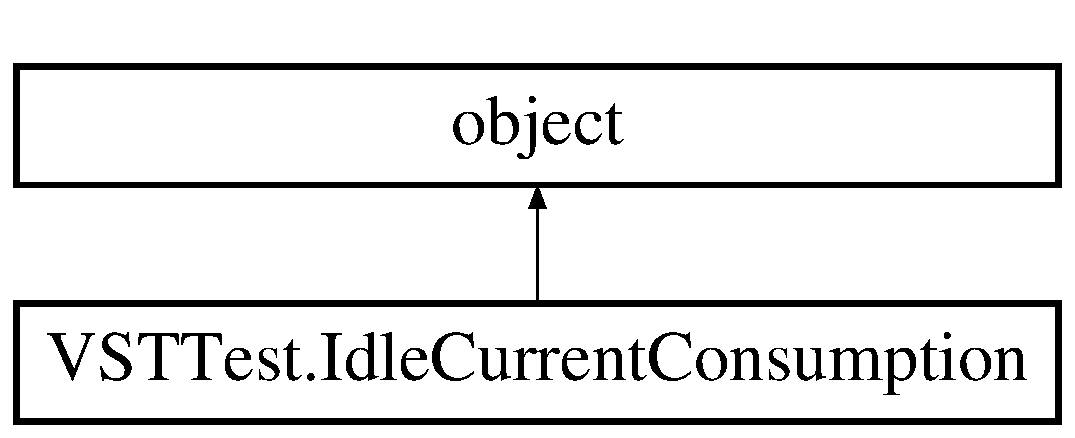
\includegraphics[height=2.000000cm]{class_v_s_t_test_1_1_idle_current_consumption}
\end{center}
\end{figure}
\subsection*{Public Member Functions}
\begin{DoxyCompactItemize}
\item 
def \hyperlink{class_v_s_t_test_1_1_idle_current_consumption_a8a0b820d03d5e6506abace8c70cd7577}{\+\_\+\+\_\+init\+\_\+\+\_\+} (self)
\begin{DoxyCompactList}\small\item\em Initialize minimum required variables for test list. \end{DoxyCompactList}\item 
def \hyperlink{class_v_s_t_test_1_1_idle_current_consumption_a39026b823531f0939cd2cd0568fdec5c}{run\+Test} (self)
\begin{DoxyCompactList}\small\item\em Run the test, save output to state variables. \end{DoxyCompactList}\item 
def \hyperlink{class_v_s_t_test_1_1_idle_current_consumption_a5c8b44240faa0975e632ce5bac14b259}{summarize} (self, summary)
\begin{DoxyCompactList}\small\item\em Summarize the test results for the cover page of the report. \end{DoxyCompactList}\item 
def \hyperlink{class_v_s_t_test_1_1_idle_current_consumption_afb740a7f4791cdf1240d84c1729fc0fc}{report} (self, pdf, report\+Path)
\begin{DoxyCompactList}\small\item\em generate this test\textquotesingle{}s page in the P\+DF report. \end{DoxyCompactList}\end{DoxyCompactItemize}


\subsection{Detailed Description}
Test for idle current consumption in the V\+ST board. 



\subsection{Constructor \& Destructor Documentation}
\index{V\+S\+T\+Test\+::\+Idle\+Current\+Consumption@{V\+S\+T\+Test\+::\+Idle\+Current\+Consumption}!\+\_\+\+\_\+init\+\_\+\+\_\+@{\+\_\+\+\_\+init\+\_\+\+\_\+}}
\index{\+\_\+\+\_\+init\+\_\+\+\_\+@{\+\_\+\+\_\+init\+\_\+\+\_\+}!V\+S\+T\+Test\+::\+Idle\+Current\+Consumption@{V\+S\+T\+Test\+::\+Idle\+Current\+Consumption}}
\subsubsection[{\texorpdfstring{\+\_\+\+\_\+init\+\_\+\+\_\+(self)}{__init__(self)}}]{\setlength{\rightskip}{0pt plus 5cm}def V\+S\+T\+Test.\+Idle\+Current\+Consumption.\+\_\+\+\_\+init\+\_\+\+\_\+ (
\begin{DoxyParamCaption}
\item[{}]{self}
\end{DoxyParamCaption}
)}\hypertarget{class_v_s_t_test_1_1_idle_current_consumption_a8a0b820d03d5e6506abace8c70cd7577}{}\label{class_v_s_t_test_1_1_idle_current_consumption_a8a0b820d03d5e6506abace8c70cd7577}


Initialize minimum required variables for test list. 



\subsection{Member Function Documentation}
\index{V\+S\+T\+Test\+::\+Idle\+Current\+Consumption@{V\+S\+T\+Test\+::\+Idle\+Current\+Consumption}!report@{report}}
\index{report@{report}!V\+S\+T\+Test\+::\+Idle\+Current\+Consumption@{V\+S\+T\+Test\+::\+Idle\+Current\+Consumption}}
\subsubsection[{\texorpdfstring{report(self, pdf, report\+Path)}{report(self, pdf, reportPath)}}]{\setlength{\rightskip}{0pt plus 5cm}def V\+S\+T\+Test.\+Idle\+Current\+Consumption.\+report (
\begin{DoxyParamCaption}
\item[{}]{self, }
\item[{}]{pdf, }
\item[{}]{report\+Path}
\end{DoxyParamCaption}
)}\hypertarget{class_v_s_t_test_1_1_idle_current_consumption_afb740a7f4791cdf1240d84c1729fc0fc}{}\label{class_v_s_t_test_1_1_idle_current_consumption_afb740a7f4791cdf1240d84c1729fc0fc}


generate this test\textquotesingle{}s page in the P\+DF report. 


\begin{DoxyParams}{Parameters}
{\em pdf} & pyfpdf-\/compatible P\+DF object. \\
\hline
{\em report\+Path} & Path of directory containing the pdf report \\
\hline
\end{DoxyParams}
\index{V\+S\+T\+Test\+::\+Idle\+Current\+Consumption@{V\+S\+T\+Test\+::\+Idle\+Current\+Consumption}!run\+Test@{run\+Test}}
\index{run\+Test@{run\+Test}!V\+S\+T\+Test\+::\+Idle\+Current\+Consumption@{V\+S\+T\+Test\+::\+Idle\+Current\+Consumption}}
\subsubsection[{\texorpdfstring{run\+Test(self)}{runTest(self)}}]{\setlength{\rightskip}{0pt plus 5cm}def V\+S\+T\+Test.\+Idle\+Current\+Consumption.\+run\+Test (
\begin{DoxyParamCaption}
\item[{}]{self}
\end{DoxyParamCaption}
)}\hypertarget{class_v_s_t_test_1_1_idle_current_consumption_a39026b823531f0939cd2cd0568fdec5c}{}\label{class_v_s_t_test_1_1_idle_current_consumption_a39026b823531f0939cd2cd0568fdec5c}


Run the test, save output to state variables. 

\index{V\+S\+T\+Test\+::\+Idle\+Current\+Consumption@{V\+S\+T\+Test\+::\+Idle\+Current\+Consumption}!summarize@{summarize}}
\index{summarize@{summarize}!V\+S\+T\+Test\+::\+Idle\+Current\+Consumption@{V\+S\+T\+Test\+::\+Idle\+Current\+Consumption}}
\subsubsection[{\texorpdfstring{summarize(self, summary)}{summarize(self, summary)}}]{\setlength{\rightskip}{0pt plus 5cm}def V\+S\+T\+Test.\+Idle\+Current\+Consumption.\+summarize (
\begin{DoxyParamCaption}
\item[{}]{self, }
\item[{}]{summary}
\end{DoxyParamCaption}
)}\hypertarget{class_v_s_t_test_1_1_idle_current_consumption_a5c8b44240faa0975e632ce5bac14b259}{}\label{class_v_s_t_test_1_1_idle_current_consumption_a5c8b44240faa0975e632ce5bac14b259}


Summarize the test results for the cover page of the report. 


\begin{DoxyParams}{Parameters}
{\em summary} & \hyperlink{class_v_s_t_test_1_1_summary}{Summary} obejct passed from Functional\+Test() \\
\hline
\end{DoxyParams}


The documentation for this class was generated from the following file\+:\begin{DoxyCompactItemize}
\item 
\hyperlink{_v_s_t_test_8py}{V\+S\+T\+Test.\+py}\end{DoxyCompactItemize}

\hypertarget{classdeprecated_1_1_jython_interface}{}\section{deprecated.\+Jython\+Interface Class Reference}
\label{classdeprecated_1_1_jython_interface}\index{deprecated.\+Jython\+Interface@{deprecated.\+Jython\+Interface}}


Some hacky workarounds to clean up the limited communication with the Jython interface.  


Inheritance diagram for deprecated.\+Jython\+Interface\+:\begin{figure}[H]
\begin{center}
\leavevmode
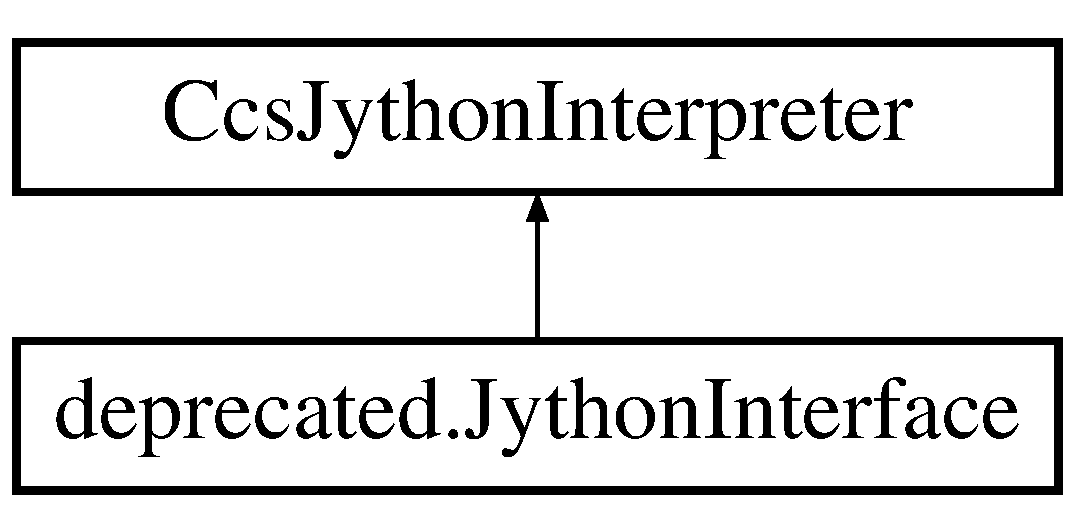
\includegraphics[height=2.000000cm]{classdeprecated_1_1_jython_interface}
\end{center}
\end{figure}
\subsection*{Public Member Functions}
\begin{DoxyCompactItemize}
\item 
def \hyperlink{classdeprecated_1_1_jython_interface_a0cd1c2bab5f66d4d34069a330b1a1303}{do} (self, code)
\begin{DoxyCompactList}\small\item\em Execute a command on the C\+CS Jython interpreter. \end{DoxyCompactList}\item 
def \hyperlink{classdeprecated_1_1_jython_interface_addcd57aa8723240416239dd13ba5940e}{get} (self, code, dtype=\char`\"{}float\char`\"{})
\begin{DoxyCompactList}\small\item\em Executes a piece of code and returns the value through get\+Output(). \end{DoxyCompactList}\end{DoxyCompactItemize}


\subsection{Detailed Description}
Some hacky workarounds to clean up the limited communication with the Jython interface. 



\subsection{Member Function Documentation}
\index{deprecated\+::\+Jython\+Interface@{deprecated\+::\+Jython\+Interface}!do@{do}}
\index{do@{do}!deprecated\+::\+Jython\+Interface@{deprecated\+::\+Jython\+Interface}}
\subsubsection[{\texorpdfstring{do(self, code)}{do(self, code)}}]{\setlength{\rightskip}{0pt plus 5cm}def deprecated.\+Jython\+Interface.\+do (
\begin{DoxyParamCaption}
\item[{}]{self, }
\item[{}]{code}
\end{DoxyParamCaption}
)}\hypertarget{classdeprecated_1_1_jython_interface_a0cd1c2bab5f66d4d34069a330b1a1303}{}\label{classdeprecated_1_1_jython_interface_a0cd1c2bab5f66d4d34069a330b1a1303}


Execute a command on the C\+CS Jython interpreter. 


\begin{DoxyParams}{Parameters}
{\em code} & Code as a literal to be executed. \\
\hline
\end{DoxyParams}
\index{deprecated\+::\+Jython\+Interface@{deprecated\+::\+Jython\+Interface}!get@{get}}
\index{get@{get}!deprecated\+::\+Jython\+Interface@{deprecated\+::\+Jython\+Interface}}
\subsubsection[{\texorpdfstring{get(self, code, dtype=""float"")}{get(self, code, dtype="float")}}]{\setlength{\rightskip}{0pt plus 5cm}def deprecated.\+Jython\+Interface.\+get (
\begin{DoxyParamCaption}
\item[{}]{self, }
\item[{}]{code, }
\item[{}]{dtype = {\ttfamily \char`\"{}float\char`\"{}}}
\end{DoxyParamCaption}
)}\hypertarget{classdeprecated_1_1_jython_interface_addcd57aa8723240416239dd13ba5940e}{}\label{classdeprecated_1_1_jython_interface_addcd57aa8723240416239dd13ba5940e}


Executes a piece of code and returns the value through get\+Output(). 


\begin{DoxyParams}{Parameters}
{\em code} & Code as a literal to be executed. \\
\hline
{\em dtype} & Optional data type, defaults to float. \\
\hline
\end{DoxyParams}
\begin{DoxyReturn}{Returns}
Converted value received through printed output from get\+Output(). get\+Output() normally only returns the results of cout, so the result is automatically typecasted to type dtype. This should be used only with a single command at a time. Like I said, hacky work around, this should be fixed in the future. 
\end{DoxyReturn}


The documentation for this class was generated from the following file\+:\begin{DoxyCompactItemize}
\item 
deprecated.\+R\+E\+B\+Test.\+py\end{DoxyCompactItemize}

\hypertarget{class_w_r_e_b_test_1_1_jython_interface}{}\section{W\+R\+E\+B\+Test.\+Jython\+Interface Class Reference}
\label{class_w_r_e_b_test_1_1_jython_interface}\index{W\+R\+E\+B\+Test.\+Jython\+Interface@{W\+R\+E\+B\+Test.\+Jython\+Interface}}


Some hacky workarounds to clean up the limited communication with the Jython interface.  


Inheritance diagram for W\+R\+E\+B\+Test.\+Jython\+Interface\+:\begin{figure}[H]
\begin{center}
\leavevmode
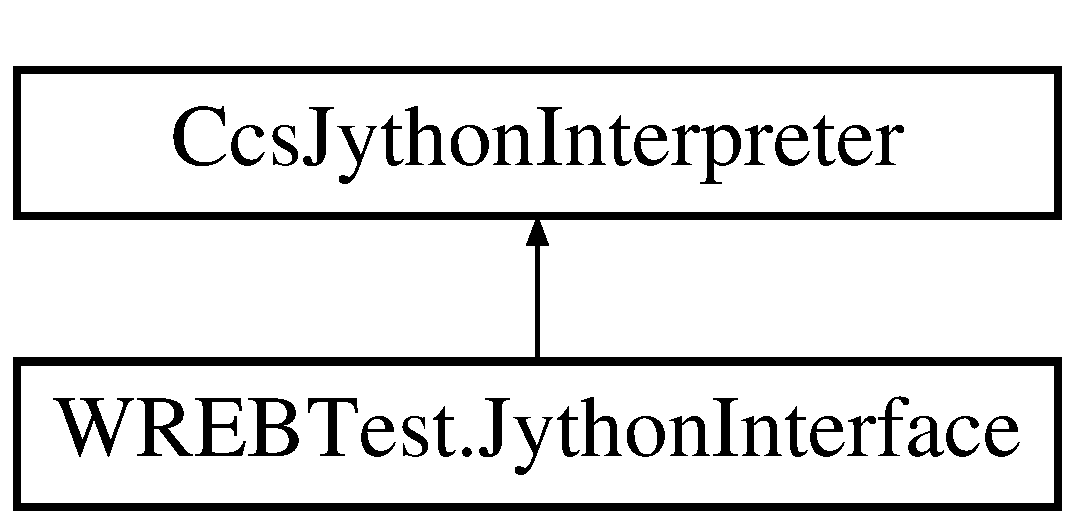
\includegraphics[height=2.000000cm]{class_w_r_e_b_test_1_1_jython_interface}
\end{center}
\end{figure}
\subsection*{Public Member Functions}
\begin{DoxyCompactItemize}
\item 
def \hyperlink{class_w_r_e_b_test_1_1_jython_interface_aaff9cae5e3c5367b1c79f8be5f087181}{do} (self, code)
\begin{DoxyCompactList}\small\item\em Execute a command on the C\+CS Jython interpreter. \end{DoxyCompactList}\item 
def \hyperlink{class_w_r_e_b_test_1_1_jython_interface_a0c3b2841fae79791193be63ac323b46a}{get} (self, code, dtype=\char`\"{}float\char`\"{})
\begin{DoxyCompactList}\small\item\em Executes a piece of code and returns the value through get\+Output(). \end{DoxyCompactList}\end{DoxyCompactItemize}


\subsection{Detailed Description}
Some hacky workarounds to clean up the limited communication with the Jython interface. 



\subsection{Member Function Documentation}
\index{W\+R\+E\+B\+Test\+::\+Jython\+Interface@{W\+R\+E\+B\+Test\+::\+Jython\+Interface}!do@{do}}
\index{do@{do}!W\+R\+E\+B\+Test\+::\+Jython\+Interface@{W\+R\+E\+B\+Test\+::\+Jython\+Interface}}
\subsubsection[{\texorpdfstring{do(self, code)}{do(self, code)}}]{\setlength{\rightskip}{0pt plus 5cm}def W\+R\+E\+B\+Test.\+Jython\+Interface.\+do (
\begin{DoxyParamCaption}
\item[{}]{self, }
\item[{}]{code}
\end{DoxyParamCaption}
)}\hypertarget{class_w_r_e_b_test_1_1_jython_interface_aaff9cae5e3c5367b1c79f8be5f087181}{}\label{class_w_r_e_b_test_1_1_jython_interface_aaff9cae5e3c5367b1c79f8be5f087181}


Execute a command on the C\+CS Jython interpreter. 


\begin{DoxyParams}{Parameters}
{\em code} & Code as a literal to be executed. \\
\hline
\end{DoxyParams}
\index{W\+R\+E\+B\+Test\+::\+Jython\+Interface@{W\+R\+E\+B\+Test\+::\+Jython\+Interface}!get@{get}}
\index{get@{get}!W\+R\+E\+B\+Test\+::\+Jython\+Interface@{W\+R\+E\+B\+Test\+::\+Jython\+Interface}}
\subsubsection[{\texorpdfstring{get(self, code, dtype=""float"")}{get(self, code, dtype="float")}}]{\setlength{\rightskip}{0pt plus 5cm}def W\+R\+E\+B\+Test.\+Jython\+Interface.\+get (
\begin{DoxyParamCaption}
\item[{}]{self, }
\item[{}]{code, }
\item[{}]{dtype = {\ttfamily \char`\"{}float\char`\"{}}}
\end{DoxyParamCaption}
)}\hypertarget{class_w_r_e_b_test_1_1_jython_interface_a0c3b2841fae79791193be63ac323b46a}{}\label{class_w_r_e_b_test_1_1_jython_interface_a0c3b2841fae79791193be63ac323b46a}


Executes a piece of code and returns the value through get\+Output(). 


\begin{DoxyParams}{Parameters}
{\em code} & Code as a literal to be executed. \\
\hline
{\em dtype} & Optional data type, defaults to float. \\
\hline
\end{DoxyParams}
\begin{DoxyReturn}{Returns}
Converted value received through printed output from get\+Output(). get\+Output() normally only returns the results of cout, so the result is automatically typecasted to type dtype. This should be used only with a single command at a time. Like I said, hacky work around, this should be fixed in the future. 
\end{DoxyReturn}


The documentation for this class was generated from the following file\+:\begin{DoxyCompactItemize}
\item 
\hyperlink{_w_r_e_b_test_8py}{W\+R\+E\+B\+Test.\+py}\end{DoxyCompactItemize}

\hypertarget{class_v_s_t_test_1_1_jython_interface}{}\section{V\+S\+T\+Test.\+Jython\+Interface Class Reference}
\label{class_v_s_t_test_1_1_jython_interface}\index{V\+S\+T\+Test.\+Jython\+Interface@{V\+S\+T\+Test.\+Jython\+Interface}}


Some hacky workarounds to clean up the limited communication with the Jython interface.  


Inheritance diagram for V\+S\+T\+Test.\+Jython\+Interface\+:\begin{figure}[H]
\begin{center}
\leavevmode
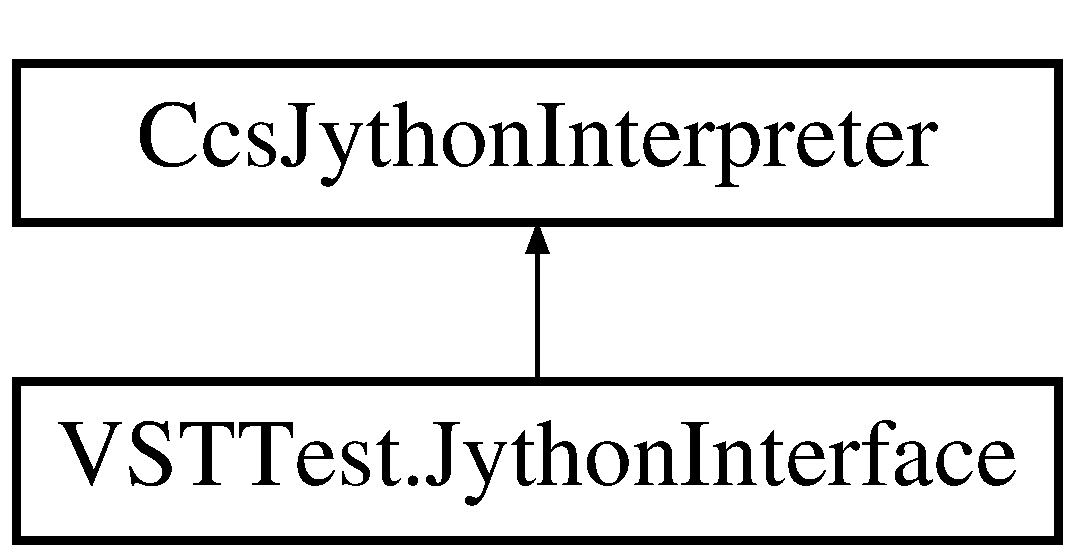
\includegraphics[height=2.000000cm]{class_v_s_t_test_1_1_jython_interface}
\end{center}
\end{figure}
\subsection*{Public Member Functions}
\begin{DoxyCompactItemize}
\item 
def \hyperlink{class_v_s_t_test_1_1_jython_interface_a15c370c16f9bace76aed9c8d1c814233}{do} (self, code)
\begin{DoxyCompactList}\small\item\em Execute a command on the C\+CS Jython interpreter. \end{DoxyCompactList}\item 
def \hyperlink{class_v_s_t_test_1_1_jython_interface_a8c33995ad28358dec6bb5ab3384fc320}{get} (self, code, dtype=\char`\"{}float\char`\"{})
\begin{DoxyCompactList}\small\item\em Executes a piece of code and returns the value through get\+Output(). \end{DoxyCompactList}\end{DoxyCompactItemize}


\subsection{Detailed Description}
Some hacky workarounds to clean up the limited communication with the Jython interface. 



\subsection{Member Function Documentation}
\index{V\+S\+T\+Test\+::\+Jython\+Interface@{V\+S\+T\+Test\+::\+Jython\+Interface}!do@{do}}
\index{do@{do}!V\+S\+T\+Test\+::\+Jython\+Interface@{V\+S\+T\+Test\+::\+Jython\+Interface}}
\subsubsection[{\texorpdfstring{do(self, code)}{do(self, code)}}]{\setlength{\rightskip}{0pt plus 5cm}def V\+S\+T\+Test.\+Jython\+Interface.\+do (
\begin{DoxyParamCaption}
\item[{}]{self, }
\item[{}]{code}
\end{DoxyParamCaption}
)}\hypertarget{class_v_s_t_test_1_1_jython_interface_a15c370c16f9bace76aed9c8d1c814233}{}\label{class_v_s_t_test_1_1_jython_interface_a15c370c16f9bace76aed9c8d1c814233}


Execute a command on the C\+CS Jython interpreter. 


\begin{DoxyParams}{Parameters}
{\em code} & Code as a literal to be executed. \\
\hline
\end{DoxyParams}
\index{V\+S\+T\+Test\+::\+Jython\+Interface@{V\+S\+T\+Test\+::\+Jython\+Interface}!get@{get}}
\index{get@{get}!V\+S\+T\+Test\+::\+Jython\+Interface@{V\+S\+T\+Test\+::\+Jython\+Interface}}
\subsubsection[{\texorpdfstring{get(self, code, dtype=""float"")}{get(self, code, dtype="float")}}]{\setlength{\rightskip}{0pt plus 5cm}def V\+S\+T\+Test.\+Jython\+Interface.\+get (
\begin{DoxyParamCaption}
\item[{}]{self, }
\item[{}]{code, }
\item[{}]{dtype = {\ttfamily \char`\"{}float\char`\"{}}}
\end{DoxyParamCaption}
)}\hypertarget{class_v_s_t_test_1_1_jython_interface_a8c33995ad28358dec6bb5ab3384fc320}{}\label{class_v_s_t_test_1_1_jython_interface_a8c33995ad28358dec6bb5ab3384fc320}


Executes a piece of code and returns the value through get\+Output(). 


\begin{DoxyParams}{Parameters}
{\em code} & Code as a literal to be executed. \\
\hline
{\em dtype} & Optional data type, defaults to float. \\
\hline
\end{DoxyParams}
\begin{DoxyReturn}{Returns}
Converted value received through printed output from get\+Output(). get\+Output() normally only returns the results of cout, so the result is automatically typecasted to type dtype. This should be used only with a single command at a time. Like I said, hacky work around, this should be fixed in the future. 
\end{DoxyReturn}


The documentation for this class was generated from the following file\+:\begin{DoxyCompactItemize}
\item 
\hyperlink{_v_s_t_test_8py}{V\+S\+T\+Test.\+py}\end{DoxyCompactItemize}

\hypertarget{class_g_r_e_b_test_1_1_jython_interface}{}\section{G\+R\+E\+B\+Test.\+Jython\+Interface Class Reference}
\label{class_g_r_e_b_test_1_1_jython_interface}\index{G\+R\+E\+B\+Test.\+Jython\+Interface@{G\+R\+E\+B\+Test.\+Jython\+Interface}}


Some hacky workarounds to clean up the limited communication with the Jython interface.  


Inheritance diagram for G\+R\+E\+B\+Test.\+Jython\+Interface\+:\begin{figure}[H]
\begin{center}
\leavevmode
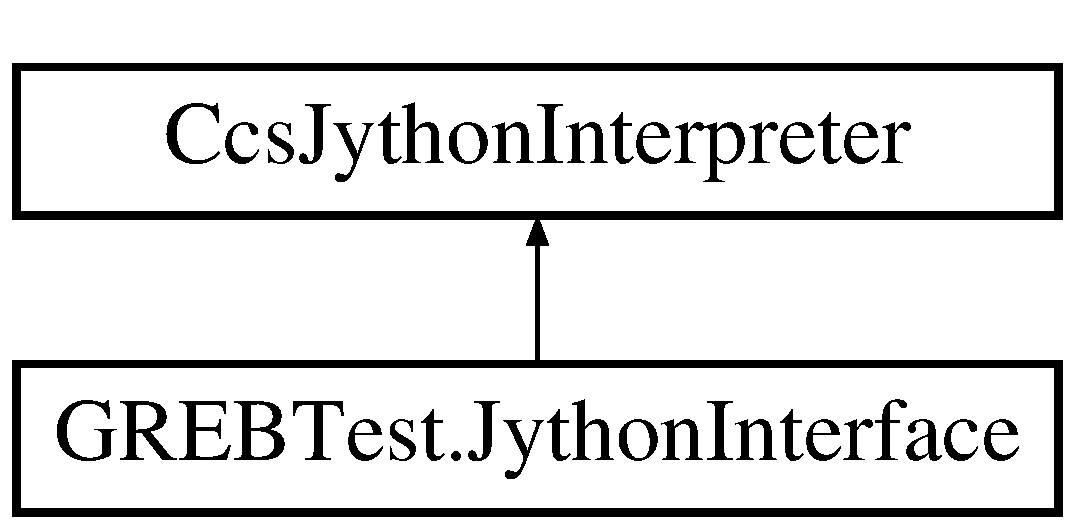
\includegraphics[height=2.000000cm]{class_g_r_e_b_test_1_1_jython_interface}
\end{center}
\end{figure}
\subsection*{Public Member Functions}
\begin{DoxyCompactItemize}
\item 
def \hyperlink{class_g_r_e_b_test_1_1_jython_interface_a8eef0a16132a249df6cc0a6e59929759}{do} (self, code)
\begin{DoxyCompactList}\small\item\em Execute a command on the C\+CS Jython interpreter. \end{DoxyCompactList}\item 
def \hyperlink{class_g_r_e_b_test_1_1_jython_interface_a5ffb7d0428e6d695cd344db062c39ed4}{get} (self, code, dtype=\char`\"{}float\char`\"{})
\begin{DoxyCompactList}\small\item\em Executes a piece of code and returns the value through get\+Output(). \end{DoxyCompactList}\end{DoxyCompactItemize}


\subsection{Detailed Description}
Some hacky workarounds to clean up the limited communication with the Jython interface. 



\subsection{Member Function Documentation}
\index{G\+R\+E\+B\+Test\+::\+Jython\+Interface@{G\+R\+E\+B\+Test\+::\+Jython\+Interface}!do@{do}}
\index{do@{do}!G\+R\+E\+B\+Test\+::\+Jython\+Interface@{G\+R\+E\+B\+Test\+::\+Jython\+Interface}}
\subsubsection[{\texorpdfstring{do(self, code)}{do(self, code)}}]{\setlength{\rightskip}{0pt plus 5cm}def G\+R\+E\+B\+Test.\+Jython\+Interface.\+do (
\begin{DoxyParamCaption}
\item[{}]{self, }
\item[{}]{code}
\end{DoxyParamCaption}
)}\hypertarget{class_g_r_e_b_test_1_1_jython_interface_a8eef0a16132a249df6cc0a6e59929759}{}\label{class_g_r_e_b_test_1_1_jython_interface_a8eef0a16132a249df6cc0a6e59929759}


Execute a command on the C\+CS Jython interpreter. 


\begin{DoxyParams}{Parameters}
{\em code} & Code as a literal to be executed. \\
\hline
\end{DoxyParams}
\index{G\+R\+E\+B\+Test\+::\+Jython\+Interface@{G\+R\+E\+B\+Test\+::\+Jython\+Interface}!get@{get}}
\index{get@{get}!G\+R\+E\+B\+Test\+::\+Jython\+Interface@{G\+R\+E\+B\+Test\+::\+Jython\+Interface}}
\subsubsection[{\texorpdfstring{get(self, code, dtype=""float"")}{get(self, code, dtype="float")}}]{\setlength{\rightskip}{0pt plus 5cm}def G\+R\+E\+B\+Test.\+Jython\+Interface.\+get (
\begin{DoxyParamCaption}
\item[{}]{self, }
\item[{}]{code, }
\item[{}]{dtype = {\ttfamily \char`\"{}float\char`\"{}}}
\end{DoxyParamCaption}
)}\hypertarget{class_g_r_e_b_test_1_1_jython_interface_a5ffb7d0428e6d695cd344db062c39ed4}{}\label{class_g_r_e_b_test_1_1_jython_interface_a5ffb7d0428e6d695cd344db062c39ed4}


Executes a piece of code and returns the value through get\+Output(). 


\begin{DoxyParams}{Parameters}
{\em code} & Code as a literal to be executed. \\
\hline
{\em dtype} & Optional data type, defaults to float. \\
\hline
\end{DoxyParams}
\begin{DoxyReturn}{Returns}
Converted value received through printed output from get\+Output(). get\+Output() normally only returns the results of cout, so the result is automatically typecasted to type dtype. This should be used only with a single command at a time. Like I said, hacky work around, this should be fixed in the future. 
\end{DoxyReturn}


The documentation for this class was generated from the following file\+:\begin{DoxyCompactItemize}
\item 
\hyperlink{_g_r_e_b_test_8py}{G\+R\+E\+B\+Test.\+py}\end{DoxyCompactItemize}

\hypertarget{class_w_r_e_b_test_1_1_o_d_bias}{}\section{W\+R\+E\+B\+Test.\+O\+D\+Bias Class Reference}
\label{class_w_r_e_b_test_1_1_o_d_bias}\index{W\+R\+E\+B\+Test.\+O\+D\+Bias@{W\+R\+E\+B\+Test.\+O\+D\+Bias}}


Tests the output drain performance.  


Inheritance diagram for W\+R\+E\+B\+Test.\+O\+D\+Bias\+:\begin{figure}[H]
\begin{center}
\leavevmode
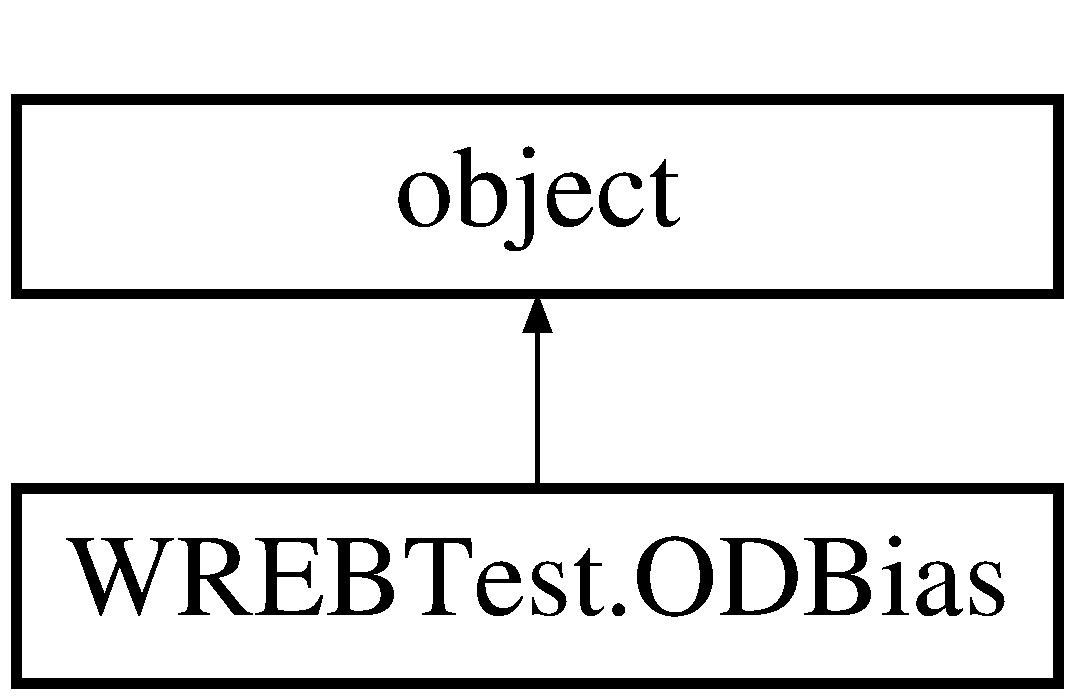
\includegraphics[height=2.000000cm]{class_w_r_e_b_test_1_1_o_d_bias}
\end{center}
\end{figure}
\subsection*{Public Member Functions}
\begin{DoxyCompactItemize}
\item 
def \hyperlink{class_w_r_e_b_test_1_1_o_d_bias_a5ab5511ac55947fbb770513f93ad86c3}{\+\_\+\+\_\+init\+\_\+\+\_\+} (self)
\begin{DoxyCompactList}\small\item\em Initialize minimum required variables for test list. \end{DoxyCompactList}\item 
def \hyperlink{class_w_r_e_b_test_1_1_o_d_bias_a70f5249d1a85164c7f3e59cad8ee23a1}{run\+Test} (self)
\begin{DoxyCompactList}\small\item\em Run the test, save output to state variables. \end{DoxyCompactList}\item 
def \hyperlink{class_w_r_e_b_test_1_1_o_d_bias_af6e5f6d44037247cc05e587cb8c8a642}{summarize} (self, summary)
\begin{DoxyCompactList}\small\item\em Summarize the test results for the cover page of the report. \end{DoxyCompactList}\item 
def \hyperlink{class_w_r_e_b_test_1_1_o_d_bias_a75f47041ae9a27789365773619cb2aad}{report} (self, pdf, report\+Path)
\begin{DoxyCompactList}\small\item\em generate this test\textquotesingle{}s page in the P\+DF report. \end{DoxyCompactList}\end{DoxyCompactItemize}


\subsection{Detailed Description}
Tests the output drain performance. 



\subsection{Constructor \& Destructor Documentation}
\index{W\+R\+E\+B\+Test\+::\+O\+D\+Bias@{W\+R\+E\+B\+Test\+::\+O\+D\+Bias}!\+\_\+\+\_\+init\+\_\+\+\_\+@{\+\_\+\+\_\+init\+\_\+\+\_\+}}
\index{\+\_\+\+\_\+init\+\_\+\+\_\+@{\+\_\+\+\_\+init\+\_\+\+\_\+}!W\+R\+E\+B\+Test\+::\+O\+D\+Bias@{W\+R\+E\+B\+Test\+::\+O\+D\+Bias}}
\subsubsection[{\texorpdfstring{\+\_\+\+\_\+init\+\_\+\+\_\+(self)}{__init__(self)}}]{\setlength{\rightskip}{0pt plus 5cm}def W\+R\+E\+B\+Test.\+O\+D\+Bias.\+\_\+\+\_\+init\+\_\+\+\_\+ (
\begin{DoxyParamCaption}
\item[{}]{self}
\end{DoxyParamCaption}
)}\hypertarget{class_w_r_e_b_test_1_1_o_d_bias_a5ab5511ac55947fbb770513f93ad86c3}{}\label{class_w_r_e_b_test_1_1_o_d_bias_a5ab5511ac55947fbb770513f93ad86c3}


Initialize minimum required variables for test list. 



\subsection{Member Function Documentation}
\index{W\+R\+E\+B\+Test\+::\+O\+D\+Bias@{W\+R\+E\+B\+Test\+::\+O\+D\+Bias}!report@{report}}
\index{report@{report}!W\+R\+E\+B\+Test\+::\+O\+D\+Bias@{W\+R\+E\+B\+Test\+::\+O\+D\+Bias}}
\subsubsection[{\texorpdfstring{report(self, pdf, report\+Path)}{report(self, pdf, reportPath)}}]{\setlength{\rightskip}{0pt plus 5cm}def W\+R\+E\+B\+Test.\+O\+D\+Bias.\+report (
\begin{DoxyParamCaption}
\item[{}]{self, }
\item[{}]{pdf, }
\item[{}]{report\+Path}
\end{DoxyParamCaption}
)}\hypertarget{class_w_r_e_b_test_1_1_o_d_bias_a75f47041ae9a27789365773619cb2aad}{}\label{class_w_r_e_b_test_1_1_o_d_bias_a75f47041ae9a27789365773619cb2aad}


generate this test\textquotesingle{}s page in the P\+DF report. 


\begin{DoxyParams}{Parameters}
{\em pdf} & pyfpdf-\/compatible P\+DF object. \\
\hline
{\em report\+Path} & Path of directory containing the pdf report \\
\hline
\end{DoxyParams}
\index{W\+R\+E\+B\+Test\+::\+O\+D\+Bias@{W\+R\+E\+B\+Test\+::\+O\+D\+Bias}!run\+Test@{run\+Test}}
\index{run\+Test@{run\+Test}!W\+R\+E\+B\+Test\+::\+O\+D\+Bias@{W\+R\+E\+B\+Test\+::\+O\+D\+Bias}}
\subsubsection[{\texorpdfstring{run\+Test(self)}{runTest(self)}}]{\setlength{\rightskip}{0pt plus 5cm}def W\+R\+E\+B\+Test.\+O\+D\+Bias.\+run\+Test (
\begin{DoxyParamCaption}
\item[{}]{self}
\end{DoxyParamCaption}
)}\hypertarget{class_w_r_e_b_test_1_1_o_d_bias_a70f5249d1a85164c7f3e59cad8ee23a1}{}\label{class_w_r_e_b_test_1_1_o_d_bias_a70f5249d1a85164c7f3e59cad8ee23a1}


Run the test, save output to state variables. 

\index{W\+R\+E\+B\+Test\+::\+O\+D\+Bias@{W\+R\+E\+B\+Test\+::\+O\+D\+Bias}!summarize@{summarize}}
\index{summarize@{summarize}!W\+R\+E\+B\+Test\+::\+O\+D\+Bias@{W\+R\+E\+B\+Test\+::\+O\+D\+Bias}}
\subsubsection[{\texorpdfstring{summarize(self, summary)}{summarize(self, summary)}}]{\setlength{\rightskip}{0pt plus 5cm}def W\+R\+E\+B\+Test.\+O\+D\+Bias.\+summarize (
\begin{DoxyParamCaption}
\item[{}]{self, }
\item[{}]{summary}
\end{DoxyParamCaption}
)}\hypertarget{class_w_r_e_b_test_1_1_o_d_bias_af6e5f6d44037247cc05e587cb8c8a642}{}\label{class_w_r_e_b_test_1_1_o_d_bias_af6e5f6d44037247cc05e587cb8c8a642}


Summarize the test results for the cover page of the report. 


\begin{DoxyParams}{Parameters}
{\em summary} & \hyperlink{class_w_r_e_b_test_1_1_summary}{Summary} obejct passed from Functional\+Test() \\
\hline
\end{DoxyParams}


The documentation for this class was generated from the following file\+:\begin{DoxyCompactItemize}
\item 
\hyperlink{_w_r_e_b_test_8py}{W\+R\+E\+B\+Test.\+py}\end{DoxyCompactItemize}

\hypertarget{class_g_r_e_b_test_1_1_o_d_bias}{}\section{G\+R\+E\+B\+Test.\+O\+D\+Bias Class Reference}
\label{class_g_r_e_b_test_1_1_o_d_bias}\index{G\+R\+E\+B\+Test.\+O\+D\+Bias@{G\+R\+E\+B\+Test.\+O\+D\+Bias}}


Tests the output drain performance.  


Inheritance diagram for G\+R\+E\+B\+Test.\+O\+D\+Bias\+:\begin{figure}[H]
\begin{center}
\leavevmode
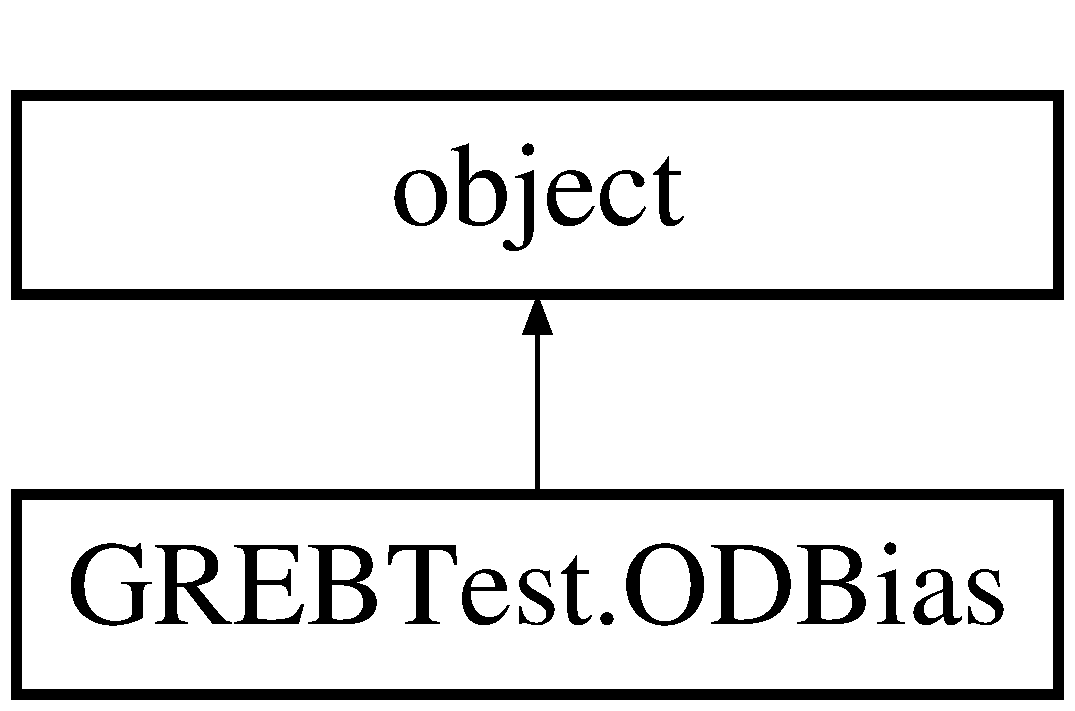
\includegraphics[height=2.000000cm]{class_g_r_e_b_test_1_1_o_d_bias}
\end{center}
\end{figure}
\subsection*{Public Member Functions}
\begin{DoxyCompactItemize}
\item 
def \hyperlink{class_g_r_e_b_test_1_1_o_d_bias_a01492c0e86e8870c15cc01c1abea62ad}{\+\_\+\+\_\+init\+\_\+\+\_\+} (self)
\begin{DoxyCompactList}\small\item\em Initialize minimum required variables for test list. \end{DoxyCompactList}\item 
def \hyperlink{class_g_r_e_b_test_1_1_o_d_bias_aa1e6d3d8892c1b8645996cf77c556c02}{run\+Test} (self)
\begin{DoxyCompactList}\small\item\em Run the test, save output to state variables. \end{DoxyCompactList}\item 
def \hyperlink{class_g_r_e_b_test_1_1_o_d_bias_a4c886d6401c18d05a81626a3a8737ab2}{summarize} (self, summary)
\begin{DoxyCompactList}\small\item\em Summarize the test results for the cover page of the report. \end{DoxyCompactList}\item 
def \hyperlink{class_g_r_e_b_test_1_1_o_d_bias_a2679f544c5633c55ba9f714d4f1d6bfb}{report} (self, pdf, report\+Path)
\begin{DoxyCompactList}\small\item\em generate this test\textquotesingle{}s page in the P\+DF report. \end{DoxyCompactList}\end{DoxyCompactItemize}


\subsection{Detailed Description}
Tests the output drain performance. 



\subsection{Constructor \& Destructor Documentation}
\index{G\+R\+E\+B\+Test\+::\+O\+D\+Bias@{G\+R\+E\+B\+Test\+::\+O\+D\+Bias}!\+\_\+\+\_\+init\+\_\+\+\_\+@{\+\_\+\+\_\+init\+\_\+\+\_\+}}
\index{\+\_\+\+\_\+init\+\_\+\+\_\+@{\+\_\+\+\_\+init\+\_\+\+\_\+}!G\+R\+E\+B\+Test\+::\+O\+D\+Bias@{G\+R\+E\+B\+Test\+::\+O\+D\+Bias}}
\subsubsection[{\texorpdfstring{\+\_\+\+\_\+init\+\_\+\+\_\+(self)}{__init__(self)}}]{\setlength{\rightskip}{0pt plus 5cm}def G\+R\+E\+B\+Test.\+O\+D\+Bias.\+\_\+\+\_\+init\+\_\+\+\_\+ (
\begin{DoxyParamCaption}
\item[{}]{self}
\end{DoxyParamCaption}
)}\hypertarget{class_g_r_e_b_test_1_1_o_d_bias_a01492c0e86e8870c15cc01c1abea62ad}{}\label{class_g_r_e_b_test_1_1_o_d_bias_a01492c0e86e8870c15cc01c1abea62ad}


Initialize minimum required variables for test list. 



\subsection{Member Function Documentation}
\index{G\+R\+E\+B\+Test\+::\+O\+D\+Bias@{G\+R\+E\+B\+Test\+::\+O\+D\+Bias}!report@{report}}
\index{report@{report}!G\+R\+E\+B\+Test\+::\+O\+D\+Bias@{G\+R\+E\+B\+Test\+::\+O\+D\+Bias}}
\subsubsection[{\texorpdfstring{report(self, pdf, report\+Path)}{report(self, pdf, reportPath)}}]{\setlength{\rightskip}{0pt plus 5cm}def G\+R\+E\+B\+Test.\+O\+D\+Bias.\+report (
\begin{DoxyParamCaption}
\item[{}]{self, }
\item[{}]{pdf, }
\item[{}]{report\+Path}
\end{DoxyParamCaption}
)}\hypertarget{class_g_r_e_b_test_1_1_o_d_bias_a2679f544c5633c55ba9f714d4f1d6bfb}{}\label{class_g_r_e_b_test_1_1_o_d_bias_a2679f544c5633c55ba9f714d4f1d6bfb}


generate this test\textquotesingle{}s page in the P\+DF report. 


\begin{DoxyParams}{Parameters}
{\em pdf} & pyfpdf-\/compatible P\+DF object. \\
\hline
{\em report\+Path} & Path of directory containing the pdf report \\
\hline
\end{DoxyParams}
\index{G\+R\+E\+B\+Test\+::\+O\+D\+Bias@{G\+R\+E\+B\+Test\+::\+O\+D\+Bias}!run\+Test@{run\+Test}}
\index{run\+Test@{run\+Test}!G\+R\+E\+B\+Test\+::\+O\+D\+Bias@{G\+R\+E\+B\+Test\+::\+O\+D\+Bias}}
\subsubsection[{\texorpdfstring{run\+Test(self)}{runTest(self)}}]{\setlength{\rightskip}{0pt plus 5cm}def G\+R\+E\+B\+Test.\+O\+D\+Bias.\+run\+Test (
\begin{DoxyParamCaption}
\item[{}]{self}
\end{DoxyParamCaption}
)}\hypertarget{class_g_r_e_b_test_1_1_o_d_bias_aa1e6d3d8892c1b8645996cf77c556c02}{}\label{class_g_r_e_b_test_1_1_o_d_bias_aa1e6d3d8892c1b8645996cf77c556c02}


Run the test, save output to state variables. 

\index{G\+R\+E\+B\+Test\+::\+O\+D\+Bias@{G\+R\+E\+B\+Test\+::\+O\+D\+Bias}!summarize@{summarize}}
\index{summarize@{summarize}!G\+R\+E\+B\+Test\+::\+O\+D\+Bias@{G\+R\+E\+B\+Test\+::\+O\+D\+Bias}}
\subsubsection[{\texorpdfstring{summarize(self, summary)}{summarize(self, summary)}}]{\setlength{\rightskip}{0pt plus 5cm}def G\+R\+E\+B\+Test.\+O\+D\+Bias.\+summarize (
\begin{DoxyParamCaption}
\item[{}]{self, }
\item[{}]{summary}
\end{DoxyParamCaption}
)}\hypertarget{class_g_r_e_b_test_1_1_o_d_bias_a4c886d6401c18d05a81626a3a8737ab2}{}\label{class_g_r_e_b_test_1_1_o_d_bias_a4c886d6401c18d05a81626a3a8737ab2}


Summarize the test results for the cover page of the report. 


\begin{DoxyParams}{Parameters}
{\em summary} & \hyperlink{class_g_r_e_b_test_1_1_summary}{Summary} obejct passed from Functional\+Test() \\
\hline
\end{DoxyParams}


The documentation for this class was generated from the following file\+:\begin{DoxyCompactItemize}
\item 
\hyperlink{_g_r_e_b_test_8py}{G\+R\+E\+B\+Test.\+py}\end{DoxyCompactItemize}

\hypertarget{class_v_s_t_test_1_1_o_d_bias}{}\section{V\+S\+T\+Test.\+O\+D\+Bias Class Reference}
\label{class_v_s_t_test_1_1_o_d_bias}\index{V\+S\+T\+Test.\+O\+D\+Bias@{V\+S\+T\+Test.\+O\+D\+Bias}}


Tests the output drain performance.  


Inheritance diagram for V\+S\+T\+Test.\+O\+D\+Bias\+:\begin{figure}[H]
\begin{center}
\leavevmode
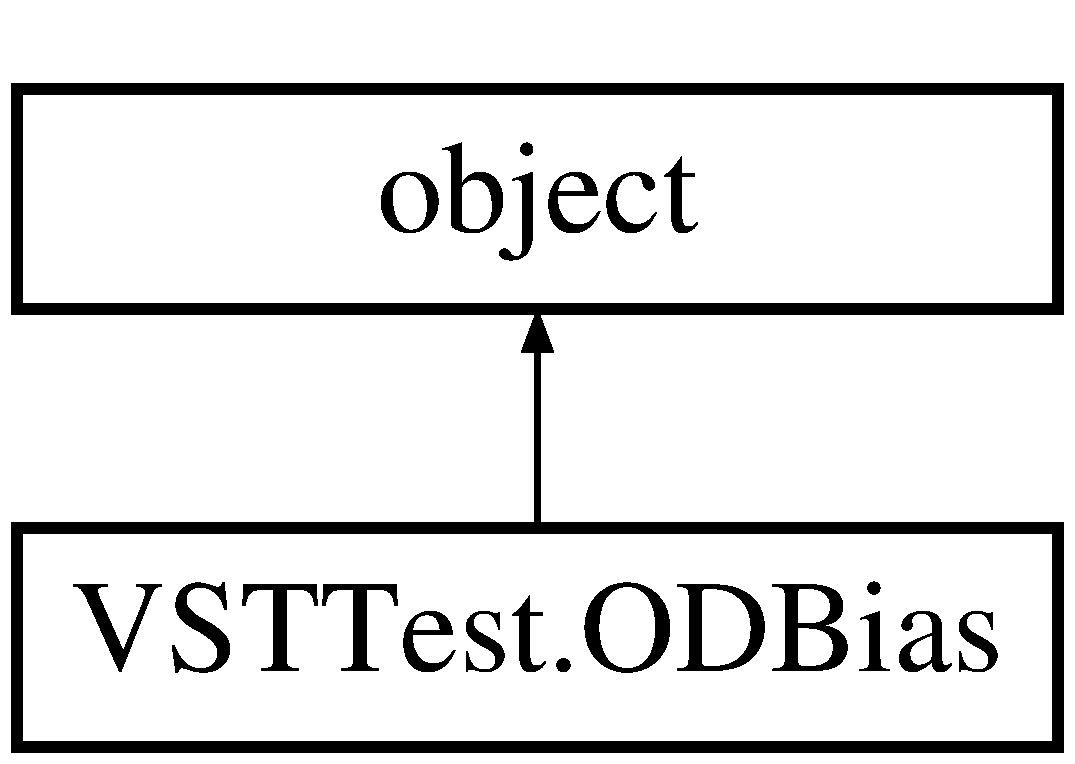
\includegraphics[height=2.000000cm]{class_v_s_t_test_1_1_o_d_bias}
\end{center}
\end{figure}
\subsection*{Public Member Functions}
\begin{DoxyCompactItemize}
\item 
def \hyperlink{class_v_s_t_test_1_1_o_d_bias_a88e2719862efb9dd56270b85f7278633}{\+\_\+\+\_\+init\+\_\+\+\_\+} (self)
\begin{DoxyCompactList}\small\item\em Initialize minimum required variables for test list. \end{DoxyCompactList}\item 
def \hyperlink{class_v_s_t_test_1_1_o_d_bias_af4171c62c482cb405b7a9f041b77b0a7}{run\+Test} (self)
\begin{DoxyCompactList}\small\item\em Run the test, save output to state variables. \end{DoxyCompactList}\item 
def \hyperlink{class_v_s_t_test_1_1_o_d_bias_a3c03e2c6ef520bbb3e816840c938d4a4}{summarize} (self, summary)
\begin{DoxyCompactList}\small\item\em Summarize the test results for the cover page of the report. \end{DoxyCompactList}\item 
def \hyperlink{class_v_s_t_test_1_1_o_d_bias_a6d831d4a581a1ec2964dcf36e2f68f61}{report} (self, pdf, report\+Path)
\begin{DoxyCompactList}\small\item\em generate this test\textquotesingle{}s page in the P\+DF report. \end{DoxyCompactList}\end{DoxyCompactItemize}


\subsection{Detailed Description}
Tests the output drain performance. 



\subsection{Constructor \& Destructor Documentation}
\index{V\+S\+T\+Test\+::\+O\+D\+Bias@{V\+S\+T\+Test\+::\+O\+D\+Bias}!\+\_\+\+\_\+init\+\_\+\+\_\+@{\+\_\+\+\_\+init\+\_\+\+\_\+}}
\index{\+\_\+\+\_\+init\+\_\+\+\_\+@{\+\_\+\+\_\+init\+\_\+\+\_\+}!V\+S\+T\+Test\+::\+O\+D\+Bias@{V\+S\+T\+Test\+::\+O\+D\+Bias}}
\subsubsection[{\texorpdfstring{\+\_\+\+\_\+init\+\_\+\+\_\+(self)}{__init__(self)}}]{\setlength{\rightskip}{0pt plus 5cm}def V\+S\+T\+Test.\+O\+D\+Bias.\+\_\+\+\_\+init\+\_\+\+\_\+ (
\begin{DoxyParamCaption}
\item[{}]{self}
\end{DoxyParamCaption}
)}\hypertarget{class_v_s_t_test_1_1_o_d_bias_a88e2719862efb9dd56270b85f7278633}{}\label{class_v_s_t_test_1_1_o_d_bias_a88e2719862efb9dd56270b85f7278633}


Initialize minimum required variables for test list. 



\subsection{Member Function Documentation}
\index{V\+S\+T\+Test\+::\+O\+D\+Bias@{V\+S\+T\+Test\+::\+O\+D\+Bias}!report@{report}}
\index{report@{report}!V\+S\+T\+Test\+::\+O\+D\+Bias@{V\+S\+T\+Test\+::\+O\+D\+Bias}}
\subsubsection[{\texorpdfstring{report(self, pdf, report\+Path)}{report(self, pdf, reportPath)}}]{\setlength{\rightskip}{0pt plus 5cm}def V\+S\+T\+Test.\+O\+D\+Bias.\+report (
\begin{DoxyParamCaption}
\item[{}]{self, }
\item[{}]{pdf, }
\item[{}]{report\+Path}
\end{DoxyParamCaption}
)}\hypertarget{class_v_s_t_test_1_1_o_d_bias_a6d831d4a581a1ec2964dcf36e2f68f61}{}\label{class_v_s_t_test_1_1_o_d_bias_a6d831d4a581a1ec2964dcf36e2f68f61}


generate this test\textquotesingle{}s page in the P\+DF report. 


\begin{DoxyParams}{Parameters}
{\em pdf} & pyfpdf-\/compatible P\+DF object. \\
\hline
{\em report\+Path} & Path of directory containing the pdf report \\
\hline
\end{DoxyParams}
\index{V\+S\+T\+Test\+::\+O\+D\+Bias@{V\+S\+T\+Test\+::\+O\+D\+Bias}!run\+Test@{run\+Test}}
\index{run\+Test@{run\+Test}!V\+S\+T\+Test\+::\+O\+D\+Bias@{V\+S\+T\+Test\+::\+O\+D\+Bias}}
\subsubsection[{\texorpdfstring{run\+Test(self)}{runTest(self)}}]{\setlength{\rightskip}{0pt plus 5cm}def V\+S\+T\+Test.\+O\+D\+Bias.\+run\+Test (
\begin{DoxyParamCaption}
\item[{}]{self}
\end{DoxyParamCaption}
)}\hypertarget{class_v_s_t_test_1_1_o_d_bias_af4171c62c482cb405b7a9f041b77b0a7}{}\label{class_v_s_t_test_1_1_o_d_bias_af4171c62c482cb405b7a9f041b77b0a7}


Run the test, save output to state variables. 

\index{V\+S\+T\+Test\+::\+O\+D\+Bias@{V\+S\+T\+Test\+::\+O\+D\+Bias}!summarize@{summarize}}
\index{summarize@{summarize}!V\+S\+T\+Test\+::\+O\+D\+Bias@{V\+S\+T\+Test\+::\+O\+D\+Bias}}
\subsubsection[{\texorpdfstring{summarize(self, summary)}{summarize(self, summary)}}]{\setlength{\rightskip}{0pt plus 5cm}def V\+S\+T\+Test.\+O\+D\+Bias.\+summarize (
\begin{DoxyParamCaption}
\item[{}]{self, }
\item[{}]{summary}
\end{DoxyParamCaption}
)}\hypertarget{class_v_s_t_test_1_1_o_d_bias_a3c03e2c6ef520bbb3e816840c938d4a4}{}\label{class_v_s_t_test_1_1_o_d_bias_a3c03e2c6ef520bbb3e816840c938d4a4}


Summarize the test results for the cover page of the report. 


\begin{DoxyParams}{Parameters}
{\em summary} & \hyperlink{class_v_s_t_test_1_1_summary}{Summary} obejct passed from Functional\+Test() \\
\hline
\end{DoxyParams}


The documentation for this class was generated from the following file\+:\begin{DoxyCompactItemize}
\item 
\hyperlink{_v_s_t_test_8py}{V\+S\+T\+Test.\+py}\end{DoxyCompactItemize}

\hypertarget{class_v_s_t_test_1_1_o_g_bias}{}\section{V\+S\+T\+Test.\+O\+G\+Bias Class Reference}
\label{class_v_s_t_test_1_1_o_g_bias}\index{V\+S\+T\+Test.\+O\+G\+Bias@{V\+S\+T\+Test.\+O\+G\+Bias}}


Tests the output gate performance.  


Inheritance diagram for V\+S\+T\+Test.\+O\+G\+Bias\+:\begin{figure}[H]
\begin{center}
\leavevmode
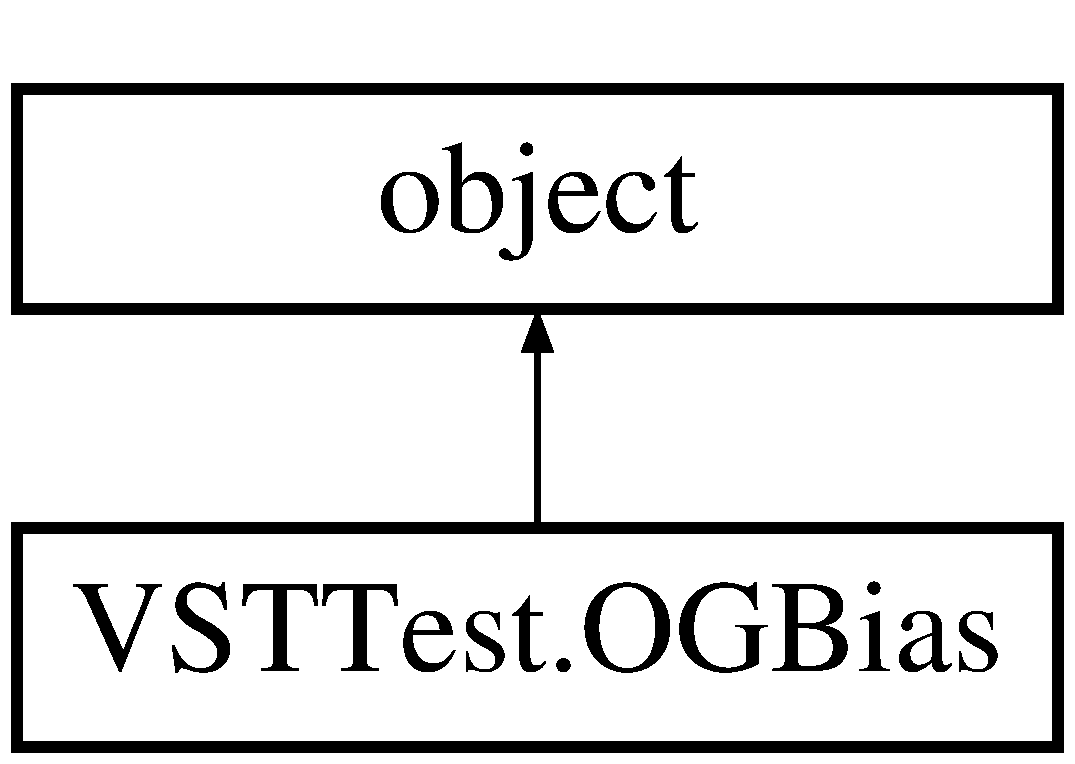
\includegraphics[height=2.000000cm]{class_v_s_t_test_1_1_o_g_bias}
\end{center}
\end{figure}
\subsection*{Public Member Functions}
\begin{DoxyCompactItemize}
\item 
def \hyperlink{class_v_s_t_test_1_1_o_g_bias_a19178d7a25a2b5230d7fcafafd000bf8}{\+\_\+\+\_\+init\+\_\+\+\_\+} (self)
\begin{DoxyCompactList}\small\item\em Initialize minimum required variables for test list. \end{DoxyCompactList}\item 
def \hyperlink{class_v_s_t_test_1_1_o_g_bias_aefb7b7ad5ddbfab605045114759dce68}{run\+Test} (self)
\begin{DoxyCompactList}\small\item\em Run the test, save output to state variables. \end{DoxyCompactList}\item 
def \hyperlink{class_v_s_t_test_1_1_o_g_bias_a9014ca0149c4800680d56f8f999d6f3c}{summarize} (self, summary)
\begin{DoxyCompactList}\small\item\em Summarize the test results for the cover page of the report. \end{DoxyCompactList}\item 
def \hyperlink{class_v_s_t_test_1_1_o_g_bias_a0d87c66621884560f08a38ec98a36153}{report} (self, pdf, report\+Path)
\begin{DoxyCompactList}\small\item\em generate this test\textquotesingle{}s page in the P\+DF report. \end{DoxyCompactList}\end{DoxyCompactItemize}


\subsection{Detailed Description}
Tests the output gate performance. 

The real OG test. 

\subsection{Constructor \& Destructor Documentation}
\index{V\+S\+T\+Test\+::\+O\+G\+Bias@{V\+S\+T\+Test\+::\+O\+G\+Bias}!\+\_\+\+\_\+init\+\_\+\+\_\+@{\+\_\+\+\_\+init\+\_\+\+\_\+}}
\index{\+\_\+\+\_\+init\+\_\+\+\_\+@{\+\_\+\+\_\+init\+\_\+\+\_\+}!V\+S\+T\+Test\+::\+O\+G\+Bias@{V\+S\+T\+Test\+::\+O\+G\+Bias}}
\subsubsection[{\texorpdfstring{\+\_\+\+\_\+init\+\_\+\+\_\+(self)}{__init__(self)}}]{\setlength{\rightskip}{0pt plus 5cm}def V\+S\+T\+Test.\+O\+G\+Bias.\+\_\+\+\_\+init\+\_\+\+\_\+ (
\begin{DoxyParamCaption}
\item[{}]{self}
\end{DoxyParamCaption}
)}\hypertarget{class_v_s_t_test_1_1_o_g_bias_a19178d7a25a2b5230d7fcafafd000bf8}{}\label{class_v_s_t_test_1_1_o_g_bias_a19178d7a25a2b5230d7fcafafd000bf8}


Initialize minimum required variables for test list. 



\subsection{Member Function Documentation}
\index{V\+S\+T\+Test\+::\+O\+G\+Bias@{V\+S\+T\+Test\+::\+O\+G\+Bias}!report@{report}}
\index{report@{report}!V\+S\+T\+Test\+::\+O\+G\+Bias@{V\+S\+T\+Test\+::\+O\+G\+Bias}}
\subsubsection[{\texorpdfstring{report(self, pdf, report\+Path)}{report(self, pdf, reportPath)}}]{\setlength{\rightskip}{0pt plus 5cm}def V\+S\+T\+Test.\+O\+G\+Bias.\+report (
\begin{DoxyParamCaption}
\item[{}]{self, }
\item[{}]{pdf, }
\item[{}]{report\+Path}
\end{DoxyParamCaption}
)}\hypertarget{class_v_s_t_test_1_1_o_g_bias_a0d87c66621884560f08a38ec98a36153}{}\label{class_v_s_t_test_1_1_o_g_bias_a0d87c66621884560f08a38ec98a36153}


generate this test\textquotesingle{}s page in the P\+DF report. 


\begin{DoxyParams}{Parameters}
{\em pdf} & pyfpdf-\/compatible P\+DF object. \\
\hline
{\em report\+Path} & Path of directory containing the pdf report \\
\hline
\end{DoxyParams}
\index{V\+S\+T\+Test\+::\+O\+G\+Bias@{V\+S\+T\+Test\+::\+O\+G\+Bias}!run\+Test@{run\+Test}}
\index{run\+Test@{run\+Test}!V\+S\+T\+Test\+::\+O\+G\+Bias@{V\+S\+T\+Test\+::\+O\+G\+Bias}}
\subsubsection[{\texorpdfstring{run\+Test(self)}{runTest(self)}}]{\setlength{\rightskip}{0pt plus 5cm}def V\+S\+T\+Test.\+O\+G\+Bias.\+run\+Test (
\begin{DoxyParamCaption}
\item[{}]{self}
\end{DoxyParamCaption}
)}\hypertarget{class_v_s_t_test_1_1_o_g_bias_aefb7b7ad5ddbfab605045114759dce68}{}\label{class_v_s_t_test_1_1_o_g_bias_aefb7b7ad5ddbfab605045114759dce68}


Run the test, save output to state variables. 

\index{V\+S\+T\+Test\+::\+O\+G\+Bias@{V\+S\+T\+Test\+::\+O\+G\+Bias}!summarize@{summarize}}
\index{summarize@{summarize}!V\+S\+T\+Test\+::\+O\+G\+Bias@{V\+S\+T\+Test\+::\+O\+G\+Bias}}
\subsubsection[{\texorpdfstring{summarize(self, summary)}{summarize(self, summary)}}]{\setlength{\rightskip}{0pt plus 5cm}def V\+S\+T\+Test.\+O\+G\+Bias.\+summarize (
\begin{DoxyParamCaption}
\item[{}]{self, }
\item[{}]{summary}
\end{DoxyParamCaption}
)}\hypertarget{class_v_s_t_test_1_1_o_g_bias_a9014ca0149c4800680d56f8f999d6f3c}{}\label{class_v_s_t_test_1_1_o_g_bias_a9014ca0149c4800680d56f8f999d6f3c}


Summarize the test results for the cover page of the report. 


\begin{DoxyParams}{Parameters}
{\em summary} & \hyperlink{class_v_s_t_test_1_1_summary}{Summary} obejct passed from Functional\+Test() \\
\hline
\end{DoxyParams}


The documentation for this class was generated from the following file\+:\begin{DoxyCompactItemize}
\item 
\hyperlink{_v_s_t_test_8py}{V\+S\+T\+Test.\+py}\end{DoxyCompactItemize}

\hypertarget{class_g_r_e_b_test_1_1_o_g_bias}{}\section{G\+R\+E\+B\+Test.\+O\+G\+Bias Class Reference}
\label{class_g_r_e_b_test_1_1_o_g_bias}\index{G\+R\+E\+B\+Test.\+O\+G\+Bias@{G\+R\+E\+B\+Test.\+O\+G\+Bias}}


Tests the output gate performance.  


Inheritance diagram for G\+R\+E\+B\+Test.\+O\+G\+Bias\+:\begin{figure}[H]
\begin{center}
\leavevmode
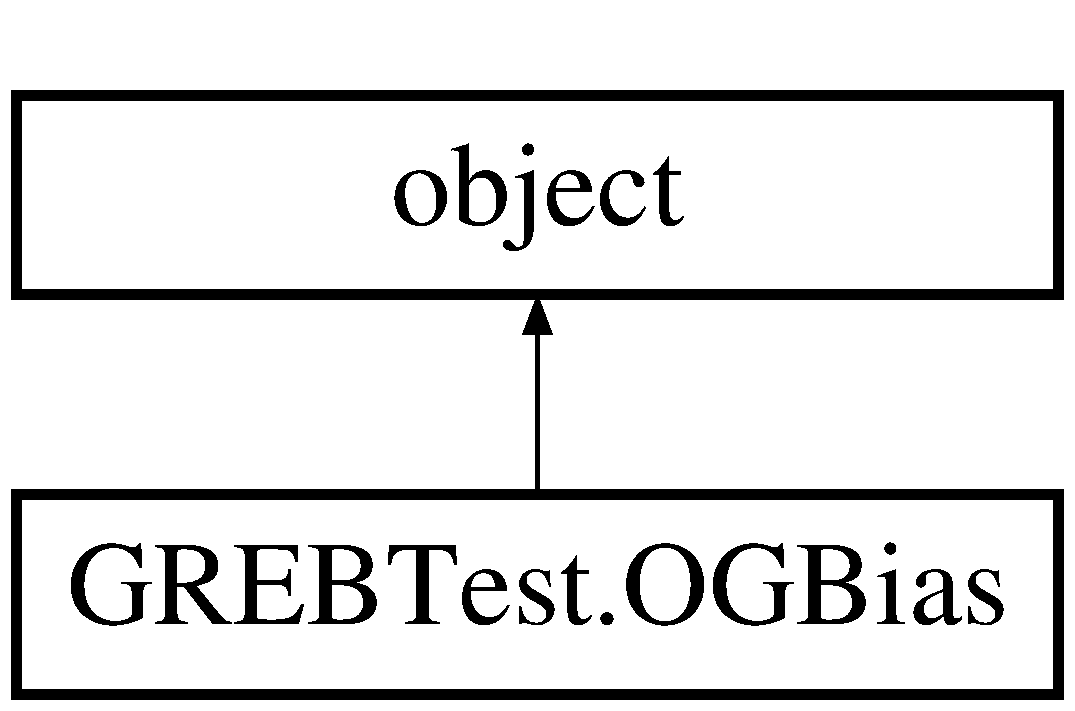
\includegraphics[height=2.000000cm]{class_g_r_e_b_test_1_1_o_g_bias}
\end{center}
\end{figure}
\subsection*{Public Member Functions}
\begin{DoxyCompactItemize}
\item 
def \hyperlink{class_g_r_e_b_test_1_1_o_g_bias_a8182fe6319290d1e1af761949871663e}{\+\_\+\+\_\+init\+\_\+\+\_\+} (self)
\begin{DoxyCompactList}\small\item\em Initialize minimum required variables for test list. \end{DoxyCompactList}\item 
def \hyperlink{class_g_r_e_b_test_1_1_o_g_bias_aaeb638ec031afb104579b968c72ee06c}{run\+Test} (self)
\begin{DoxyCompactList}\small\item\em Run the test, save output to state variables. \end{DoxyCompactList}\item 
def \hyperlink{class_g_r_e_b_test_1_1_o_g_bias_a22a9b5a43ccd76f58b6109446a34015a}{summarize} (self, summary)
\begin{DoxyCompactList}\small\item\em Summarize the test results for the cover page of the report. \end{DoxyCompactList}\item 
def \hyperlink{class_g_r_e_b_test_1_1_o_g_bias_ad0814258580f121c9ba1a5b730d9bac4}{report} (self, pdf, report\+Path)
\begin{DoxyCompactList}\small\item\em generate this test\textquotesingle{}s page in the P\+DF report. \end{DoxyCompactList}\end{DoxyCompactItemize}


\subsection{Detailed Description}
Tests the output gate performance. 

The real OG test. 

\subsection{Constructor \& Destructor Documentation}
\index{G\+R\+E\+B\+Test\+::\+O\+G\+Bias@{G\+R\+E\+B\+Test\+::\+O\+G\+Bias}!\+\_\+\+\_\+init\+\_\+\+\_\+@{\+\_\+\+\_\+init\+\_\+\+\_\+}}
\index{\+\_\+\+\_\+init\+\_\+\+\_\+@{\+\_\+\+\_\+init\+\_\+\+\_\+}!G\+R\+E\+B\+Test\+::\+O\+G\+Bias@{G\+R\+E\+B\+Test\+::\+O\+G\+Bias}}
\subsubsection[{\texorpdfstring{\+\_\+\+\_\+init\+\_\+\+\_\+(self)}{__init__(self)}}]{\setlength{\rightskip}{0pt plus 5cm}def G\+R\+E\+B\+Test.\+O\+G\+Bias.\+\_\+\+\_\+init\+\_\+\+\_\+ (
\begin{DoxyParamCaption}
\item[{}]{self}
\end{DoxyParamCaption}
)}\hypertarget{class_g_r_e_b_test_1_1_o_g_bias_a8182fe6319290d1e1af761949871663e}{}\label{class_g_r_e_b_test_1_1_o_g_bias_a8182fe6319290d1e1af761949871663e}


Initialize minimum required variables for test list. 



\subsection{Member Function Documentation}
\index{G\+R\+E\+B\+Test\+::\+O\+G\+Bias@{G\+R\+E\+B\+Test\+::\+O\+G\+Bias}!report@{report}}
\index{report@{report}!G\+R\+E\+B\+Test\+::\+O\+G\+Bias@{G\+R\+E\+B\+Test\+::\+O\+G\+Bias}}
\subsubsection[{\texorpdfstring{report(self, pdf, report\+Path)}{report(self, pdf, reportPath)}}]{\setlength{\rightskip}{0pt plus 5cm}def G\+R\+E\+B\+Test.\+O\+G\+Bias.\+report (
\begin{DoxyParamCaption}
\item[{}]{self, }
\item[{}]{pdf, }
\item[{}]{report\+Path}
\end{DoxyParamCaption}
)}\hypertarget{class_g_r_e_b_test_1_1_o_g_bias_ad0814258580f121c9ba1a5b730d9bac4}{}\label{class_g_r_e_b_test_1_1_o_g_bias_ad0814258580f121c9ba1a5b730d9bac4}


generate this test\textquotesingle{}s page in the P\+DF report. 


\begin{DoxyParams}{Parameters}
{\em pdf} & pyfpdf-\/compatible P\+DF object. \\
\hline
{\em report\+Path} & Path of directory containing the pdf report \\
\hline
\end{DoxyParams}
\index{G\+R\+E\+B\+Test\+::\+O\+G\+Bias@{G\+R\+E\+B\+Test\+::\+O\+G\+Bias}!run\+Test@{run\+Test}}
\index{run\+Test@{run\+Test}!G\+R\+E\+B\+Test\+::\+O\+G\+Bias@{G\+R\+E\+B\+Test\+::\+O\+G\+Bias}}
\subsubsection[{\texorpdfstring{run\+Test(self)}{runTest(self)}}]{\setlength{\rightskip}{0pt plus 5cm}def G\+R\+E\+B\+Test.\+O\+G\+Bias.\+run\+Test (
\begin{DoxyParamCaption}
\item[{}]{self}
\end{DoxyParamCaption}
)}\hypertarget{class_g_r_e_b_test_1_1_o_g_bias_aaeb638ec031afb104579b968c72ee06c}{}\label{class_g_r_e_b_test_1_1_o_g_bias_aaeb638ec031afb104579b968c72ee06c}


Run the test, save output to state variables. 

\index{G\+R\+E\+B\+Test\+::\+O\+G\+Bias@{G\+R\+E\+B\+Test\+::\+O\+G\+Bias}!summarize@{summarize}}
\index{summarize@{summarize}!G\+R\+E\+B\+Test\+::\+O\+G\+Bias@{G\+R\+E\+B\+Test\+::\+O\+G\+Bias}}
\subsubsection[{\texorpdfstring{summarize(self, summary)}{summarize(self, summary)}}]{\setlength{\rightskip}{0pt plus 5cm}def G\+R\+E\+B\+Test.\+O\+G\+Bias.\+summarize (
\begin{DoxyParamCaption}
\item[{}]{self, }
\item[{}]{summary}
\end{DoxyParamCaption}
)}\hypertarget{class_g_r_e_b_test_1_1_o_g_bias_a22a9b5a43ccd76f58b6109446a34015a}{}\label{class_g_r_e_b_test_1_1_o_g_bias_a22a9b5a43ccd76f58b6109446a34015a}


Summarize the test results for the cover page of the report. 


\begin{DoxyParams}{Parameters}
{\em summary} & \hyperlink{class_g_r_e_b_test_1_1_summary}{Summary} obejct passed from Functional\+Test() \\
\hline
\end{DoxyParams}


The documentation for this class was generated from the following file\+:\begin{DoxyCompactItemize}
\item 
\hyperlink{_g_r_e_b_test_8py}{G\+R\+E\+B\+Test.\+py}\end{DoxyCompactItemize}

\hypertarget{class_w_r_e_b_test_1_1_o_g_bias}{}\section{W\+R\+E\+B\+Test.\+O\+G\+Bias Class Reference}
\label{class_w_r_e_b_test_1_1_o_g_bias}\index{W\+R\+E\+B\+Test.\+O\+G\+Bias@{W\+R\+E\+B\+Test.\+O\+G\+Bias}}


Tests the output gate performance.  


Inheritance diagram for W\+R\+E\+B\+Test.\+O\+G\+Bias\+:\begin{figure}[H]
\begin{center}
\leavevmode
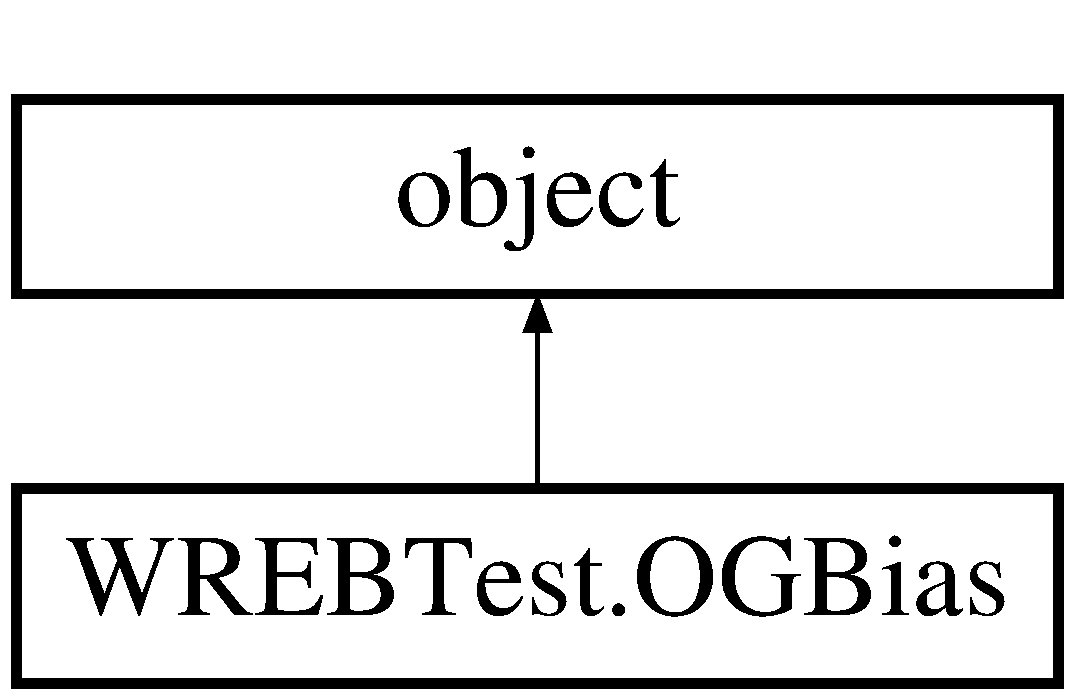
\includegraphics[height=2.000000cm]{class_w_r_e_b_test_1_1_o_g_bias}
\end{center}
\end{figure}
\subsection*{Public Member Functions}
\begin{DoxyCompactItemize}
\item 
def \hyperlink{class_w_r_e_b_test_1_1_o_g_bias_a54e5379325a6a8707049e5287b4a540b}{\+\_\+\+\_\+init\+\_\+\+\_\+} (self)
\begin{DoxyCompactList}\small\item\em Initialize minimum required variables for test list. \end{DoxyCompactList}\item 
def \hyperlink{class_w_r_e_b_test_1_1_o_g_bias_ab3882e57d4909ecab2f9a255661df21d}{run\+Test} (self)
\begin{DoxyCompactList}\small\item\em Run the test, save output to state variables. \end{DoxyCompactList}\item 
def \hyperlink{class_w_r_e_b_test_1_1_o_g_bias_a9efac6be807016d3ed4359aae56e15a8}{summarize} (self, summary)
\begin{DoxyCompactList}\small\item\em Summarize the test results for the cover page of the report. \end{DoxyCompactList}\item 
def \hyperlink{class_w_r_e_b_test_1_1_o_g_bias_a031d4b9bde53c91eeb095d19c2f5576f}{report} (self, pdf, report\+Path)
\begin{DoxyCompactList}\small\item\em generate this test\textquotesingle{}s page in the P\+DF report. \end{DoxyCompactList}\end{DoxyCompactItemize}


\subsection{Detailed Description}
Tests the output gate performance. 

The real OG test. 

\subsection{Constructor \& Destructor Documentation}
\index{W\+R\+E\+B\+Test\+::\+O\+G\+Bias@{W\+R\+E\+B\+Test\+::\+O\+G\+Bias}!\+\_\+\+\_\+init\+\_\+\+\_\+@{\+\_\+\+\_\+init\+\_\+\+\_\+}}
\index{\+\_\+\+\_\+init\+\_\+\+\_\+@{\+\_\+\+\_\+init\+\_\+\+\_\+}!W\+R\+E\+B\+Test\+::\+O\+G\+Bias@{W\+R\+E\+B\+Test\+::\+O\+G\+Bias}}
\subsubsection[{\texorpdfstring{\+\_\+\+\_\+init\+\_\+\+\_\+(self)}{__init__(self)}}]{\setlength{\rightskip}{0pt plus 5cm}def W\+R\+E\+B\+Test.\+O\+G\+Bias.\+\_\+\+\_\+init\+\_\+\+\_\+ (
\begin{DoxyParamCaption}
\item[{}]{self}
\end{DoxyParamCaption}
)}\hypertarget{class_w_r_e_b_test_1_1_o_g_bias_a54e5379325a6a8707049e5287b4a540b}{}\label{class_w_r_e_b_test_1_1_o_g_bias_a54e5379325a6a8707049e5287b4a540b}


Initialize minimum required variables for test list. 



\subsection{Member Function Documentation}
\index{W\+R\+E\+B\+Test\+::\+O\+G\+Bias@{W\+R\+E\+B\+Test\+::\+O\+G\+Bias}!report@{report}}
\index{report@{report}!W\+R\+E\+B\+Test\+::\+O\+G\+Bias@{W\+R\+E\+B\+Test\+::\+O\+G\+Bias}}
\subsubsection[{\texorpdfstring{report(self, pdf, report\+Path)}{report(self, pdf, reportPath)}}]{\setlength{\rightskip}{0pt plus 5cm}def W\+R\+E\+B\+Test.\+O\+G\+Bias.\+report (
\begin{DoxyParamCaption}
\item[{}]{self, }
\item[{}]{pdf, }
\item[{}]{report\+Path}
\end{DoxyParamCaption}
)}\hypertarget{class_w_r_e_b_test_1_1_o_g_bias_a031d4b9bde53c91eeb095d19c2f5576f}{}\label{class_w_r_e_b_test_1_1_o_g_bias_a031d4b9bde53c91eeb095d19c2f5576f}


generate this test\textquotesingle{}s page in the P\+DF report. 


\begin{DoxyParams}{Parameters}
{\em pdf} & pyfpdf-\/compatible P\+DF object. \\
\hline
{\em report\+Path} & Path of directory containing the pdf report \\
\hline
\end{DoxyParams}
\index{W\+R\+E\+B\+Test\+::\+O\+G\+Bias@{W\+R\+E\+B\+Test\+::\+O\+G\+Bias}!run\+Test@{run\+Test}}
\index{run\+Test@{run\+Test}!W\+R\+E\+B\+Test\+::\+O\+G\+Bias@{W\+R\+E\+B\+Test\+::\+O\+G\+Bias}}
\subsubsection[{\texorpdfstring{run\+Test(self)}{runTest(self)}}]{\setlength{\rightskip}{0pt plus 5cm}def W\+R\+E\+B\+Test.\+O\+G\+Bias.\+run\+Test (
\begin{DoxyParamCaption}
\item[{}]{self}
\end{DoxyParamCaption}
)}\hypertarget{class_w_r_e_b_test_1_1_o_g_bias_ab3882e57d4909ecab2f9a255661df21d}{}\label{class_w_r_e_b_test_1_1_o_g_bias_ab3882e57d4909ecab2f9a255661df21d}


Run the test, save output to state variables. 

\index{W\+R\+E\+B\+Test\+::\+O\+G\+Bias@{W\+R\+E\+B\+Test\+::\+O\+G\+Bias}!summarize@{summarize}}
\index{summarize@{summarize}!W\+R\+E\+B\+Test\+::\+O\+G\+Bias@{W\+R\+E\+B\+Test\+::\+O\+G\+Bias}}
\subsubsection[{\texorpdfstring{summarize(self, summary)}{summarize(self, summary)}}]{\setlength{\rightskip}{0pt plus 5cm}def W\+R\+E\+B\+Test.\+O\+G\+Bias.\+summarize (
\begin{DoxyParamCaption}
\item[{}]{self, }
\item[{}]{summary}
\end{DoxyParamCaption}
)}\hypertarget{class_w_r_e_b_test_1_1_o_g_bias_a9efac6be807016d3ed4359aae56e15a8}{}\label{class_w_r_e_b_test_1_1_o_g_bias_a9efac6be807016d3ed4359aae56e15a8}


Summarize the test results for the cover page of the report. 


\begin{DoxyParams}{Parameters}
{\em summary} & \hyperlink{class_w_r_e_b_test_1_1_summary}{Summary} obejct passed from Functional\+Test() \\
\hline
\end{DoxyParams}


The documentation for this class was generated from the following file\+:\begin{DoxyCompactItemize}
\item 
\hyperlink{_w_r_e_b_test_8py}{W\+R\+E\+B\+Test.\+py}\end{DoxyCompactItemize}

\hypertarget{class_g_r_e_b_test_1_1_parameter_logging}{}\section{G\+R\+E\+B\+Test.\+Parameter\+Logging Class Reference}
\label{class_g_r_e_b_test_1_1_parameter_logging}\index{G\+R\+E\+B\+Test.\+Parameter\+Logging@{G\+R\+E\+B\+Test.\+Parameter\+Logging}}


Periodically records specified values over the course of the testing sequence.  


Inheritance diagram for G\+R\+E\+B\+Test.\+Parameter\+Logging\+:\begin{figure}[H]
\begin{center}
\leavevmode
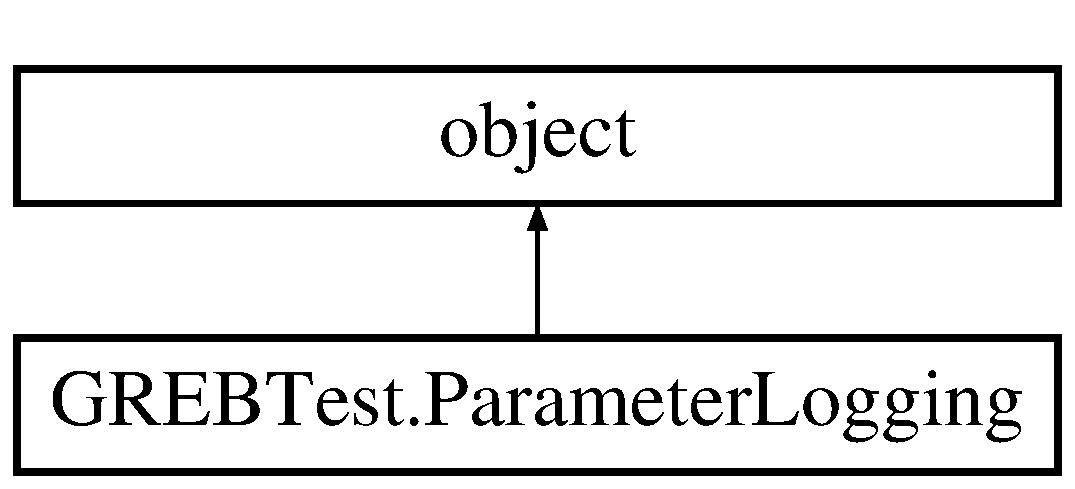
\includegraphics[height=2.000000cm]{class_g_r_e_b_test_1_1_parameter_logging}
\end{center}
\end{figure}
\subsection*{Public Member Functions}
\begin{DoxyCompactItemize}
\item 
def \hyperlink{class_g_r_e_b_test_1_1_parameter_logging_a9f4b5fea65ed9d1b1ead8c998e55e7d9}{\+\_\+\+\_\+init\+\_\+\+\_\+} (self, values\+To\+Read, delay=5, fn\+Test=None, backup=0)
\begin{DoxyCompactList}\small\item\em Initializes the test. \end{DoxyCompactList}\item 
def \hyperlink{class_g_r_e_b_test_1_1_parameter_logging_aa17135431592e8e48d6beef5bdf69bf7}{run\+Test} (self)
\begin{DoxyCompactList}\small\item\em Starts the logging in a separate thread, moves to the next test. \end{DoxyCompactList}\item 
def \hyperlink{class_g_r_e_b_test_1_1_parameter_logging_af0371ffd21126c1c792feeb48f6f0f50}{stop\+Test} (self)
\begin{DoxyCompactList}\small\item\em Sets the recording option to false, allowing the test to stop. \end{DoxyCompactList}\item 
def \hyperlink{class_g_r_e_b_test_1_1_parameter_logging_af29d8e244da00678d07584abd2aa6973}{record\+Continuously} (self)
\begin{DoxyCompactList}\small\item\em Continuously records the requested parameters while self.\+recording is set to true. \end{DoxyCompactList}\item 
def \hyperlink{class_g_r_e_b_test_1_1_parameter_logging_a490fb25836f3c8eccb514d165798e995}{pass\+Fail} (self)
\begin{DoxyCompactList}\small\item\em Determine if the value logging passed -\/ this is done in a separate function, unlike other tests. \end{DoxyCompactList}\item 
def \hyperlink{class_g_r_e_b_test_1_1_parameter_logging_aab5129de996e3ff7735676f208b1c9cd}{report} (self, pdf, report\+Path)
\begin{DoxyCompactList}\small\item\em generate this test\textquotesingle{}s page in the P\+DF report. \end{DoxyCompactList}\end{DoxyCompactItemize}


\subsection{Detailed Description}
Periodically records specified values over the course of the testing sequence. 



\subsection{Constructor \& Destructor Documentation}
\index{G\+R\+E\+B\+Test\+::\+Parameter\+Logging@{G\+R\+E\+B\+Test\+::\+Parameter\+Logging}!\+\_\+\+\_\+init\+\_\+\+\_\+@{\+\_\+\+\_\+init\+\_\+\+\_\+}}
\index{\+\_\+\+\_\+init\+\_\+\+\_\+@{\+\_\+\+\_\+init\+\_\+\+\_\+}!G\+R\+E\+B\+Test\+::\+Parameter\+Logging@{G\+R\+E\+B\+Test\+::\+Parameter\+Logging}}
\subsubsection[{\texorpdfstring{\+\_\+\+\_\+init\+\_\+\+\_\+(self, values\+To\+Read, delay=5, fn\+Test=\+None, backup=0)}{__init__(self, valuesToRead, delay=5, fnTest=None, backup=0)}}]{\setlength{\rightskip}{0pt plus 5cm}def G\+R\+E\+B\+Test.\+Parameter\+Logging.\+\_\+\+\_\+init\+\_\+\+\_\+ (
\begin{DoxyParamCaption}
\item[{}]{self, }
\item[{}]{values\+To\+Read, }
\item[{}]{delay = {\ttfamily 5}, }
\item[{}]{fn\+Test = {\ttfamily None}, }
\item[{}]{backup = {\ttfamily 0}}
\end{DoxyParamCaption}
)}\hypertarget{class_g_r_e_b_test_1_1_parameter_logging_a9f4b5fea65ed9d1b1ead8c998e55e7d9}{}\label{class_g_r_e_b_test_1_1_parameter_logging_a9f4b5fea65ed9d1b1ead8c998e55e7d9}


Initializes the test. 


\begin{DoxyParams}{Parameters}
{\em values\+To\+Read} & A list of (\char`\"{}subsystem\char`\"{}, \char`\"{}value to read\char`\"{}) tuples \\
\hline
{\em delay} & Time to sleep between periodic queries \\
\hline
{\em fn\+Test} & The Functional\+Test() object, allowing this test to track progress/terminate \\
\hline
{\em backup} & Backup data every n cycles. If zero, do not back up. \\
\hline
\end{DoxyParams}


\subsection{Member Function Documentation}
\index{G\+R\+E\+B\+Test\+::\+Parameter\+Logging@{G\+R\+E\+B\+Test\+::\+Parameter\+Logging}!pass\+Fail@{pass\+Fail}}
\index{pass\+Fail@{pass\+Fail}!G\+R\+E\+B\+Test\+::\+Parameter\+Logging@{G\+R\+E\+B\+Test\+::\+Parameter\+Logging}}
\subsubsection[{\texorpdfstring{pass\+Fail(self)}{passFail(self)}}]{\setlength{\rightskip}{0pt plus 5cm}def G\+R\+E\+B\+Test.\+Parameter\+Logging.\+pass\+Fail (
\begin{DoxyParamCaption}
\item[{}]{self}
\end{DoxyParamCaption}
)}\hypertarget{class_g_r_e_b_test_1_1_parameter_logging_a490fb25836f3c8eccb514d165798e995}{}\label{class_g_r_e_b_test_1_1_parameter_logging_a490fb25836f3c8eccb514d165798e995}


Determine if the value logging passed -\/ this is done in a separate function, unlike other tests. 

\index{G\+R\+E\+B\+Test\+::\+Parameter\+Logging@{G\+R\+E\+B\+Test\+::\+Parameter\+Logging}!record\+Continuously@{record\+Continuously}}
\index{record\+Continuously@{record\+Continuously}!G\+R\+E\+B\+Test\+::\+Parameter\+Logging@{G\+R\+E\+B\+Test\+::\+Parameter\+Logging}}
\subsubsection[{\texorpdfstring{record\+Continuously(self)}{recordContinuously(self)}}]{\setlength{\rightskip}{0pt plus 5cm}def G\+R\+E\+B\+Test.\+Parameter\+Logging.\+record\+Continuously (
\begin{DoxyParamCaption}
\item[{}]{self}
\end{DoxyParamCaption}
)}\hypertarget{class_g_r_e_b_test_1_1_parameter_logging_af29d8e244da00678d07584abd2aa6973}{}\label{class_g_r_e_b_test_1_1_parameter_logging_af29d8e244da00678d07584abd2aa6973}


Continuously records the requested parameters while self.\+recording is set to true. 

\index{G\+R\+E\+B\+Test\+::\+Parameter\+Logging@{G\+R\+E\+B\+Test\+::\+Parameter\+Logging}!report@{report}}
\index{report@{report}!G\+R\+E\+B\+Test\+::\+Parameter\+Logging@{G\+R\+E\+B\+Test\+::\+Parameter\+Logging}}
\subsubsection[{\texorpdfstring{report(self, pdf, report\+Path)}{report(self, pdf, reportPath)}}]{\setlength{\rightskip}{0pt plus 5cm}def G\+R\+E\+B\+Test.\+Parameter\+Logging.\+report (
\begin{DoxyParamCaption}
\item[{}]{self, }
\item[{}]{pdf, }
\item[{}]{report\+Path}
\end{DoxyParamCaption}
)}\hypertarget{class_g_r_e_b_test_1_1_parameter_logging_aab5129de996e3ff7735676f208b1c9cd}{}\label{class_g_r_e_b_test_1_1_parameter_logging_aab5129de996e3ff7735676f208b1c9cd}


generate this test\textquotesingle{}s page in the P\+DF report. 


\begin{DoxyParams}{Parameters}
{\em pdf} & pyfpdf-\/compatible P\+DF object. \\
\hline
{\em report\+Path} & Path of directory containing the pdf report \\
\hline
\end{DoxyParams}
\index{G\+R\+E\+B\+Test\+::\+Parameter\+Logging@{G\+R\+E\+B\+Test\+::\+Parameter\+Logging}!run\+Test@{run\+Test}}
\index{run\+Test@{run\+Test}!G\+R\+E\+B\+Test\+::\+Parameter\+Logging@{G\+R\+E\+B\+Test\+::\+Parameter\+Logging}}
\subsubsection[{\texorpdfstring{run\+Test(self)}{runTest(self)}}]{\setlength{\rightskip}{0pt plus 5cm}def G\+R\+E\+B\+Test.\+Parameter\+Logging.\+run\+Test (
\begin{DoxyParamCaption}
\item[{}]{self}
\end{DoxyParamCaption}
)}\hypertarget{class_g_r_e_b_test_1_1_parameter_logging_aa17135431592e8e48d6beef5bdf69bf7}{}\label{class_g_r_e_b_test_1_1_parameter_logging_aa17135431592e8e48d6beef5bdf69bf7}


Starts the logging in a separate thread, moves to the next test. 

\index{G\+R\+E\+B\+Test\+::\+Parameter\+Logging@{G\+R\+E\+B\+Test\+::\+Parameter\+Logging}!stop\+Test@{stop\+Test}}
\index{stop\+Test@{stop\+Test}!G\+R\+E\+B\+Test\+::\+Parameter\+Logging@{G\+R\+E\+B\+Test\+::\+Parameter\+Logging}}
\subsubsection[{\texorpdfstring{stop\+Test(self)}{stopTest(self)}}]{\setlength{\rightskip}{0pt plus 5cm}def G\+R\+E\+B\+Test.\+Parameter\+Logging.\+stop\+Test (
\begin{DoxyParamCaption}
\item[{}]{self}
\end{DoxyParamCaption}
)}\hypertarget{class_g_r_e_b_test_1_1_parameter_logging_af0371ffd21126c1c792feeb48f6f0f50}{}\label{class_g_r_e_b_test_1_1_parameter_logging_af0371ffd21126c1c792feeb48f6f0f50}


Sets the recording option to false, allowing the test to stop. 



The documentation for this class was generated from the following file\+:\begin{DoxyCompactItemize}
\item 
\hyperlink{_g_r_e_b_test_8py}{G\+R\+E\+B\+Test.\+py}\end{DoxyCompactItemize}

\hypertarget{class_v_s_t_test_1_1_parameter_logging}{}\section{V\+S\+T\+Test.\+Parameter\+Logging Class Reference}
\label{class_v_s_t_test_1_1_parameter_logging}\index{V\+S\+T\+Test.\+Parameter\+Logging@{V\+S\+T\+Test.\+Parameter\+Logging}}


Periodically records specified values over the course of the testing sequence.  


Inheritance diagram for V\+S\+T\+Test.\+Parameter\+Logging\+:\begin{figure}[H]
\begin{center}
\leavevmode
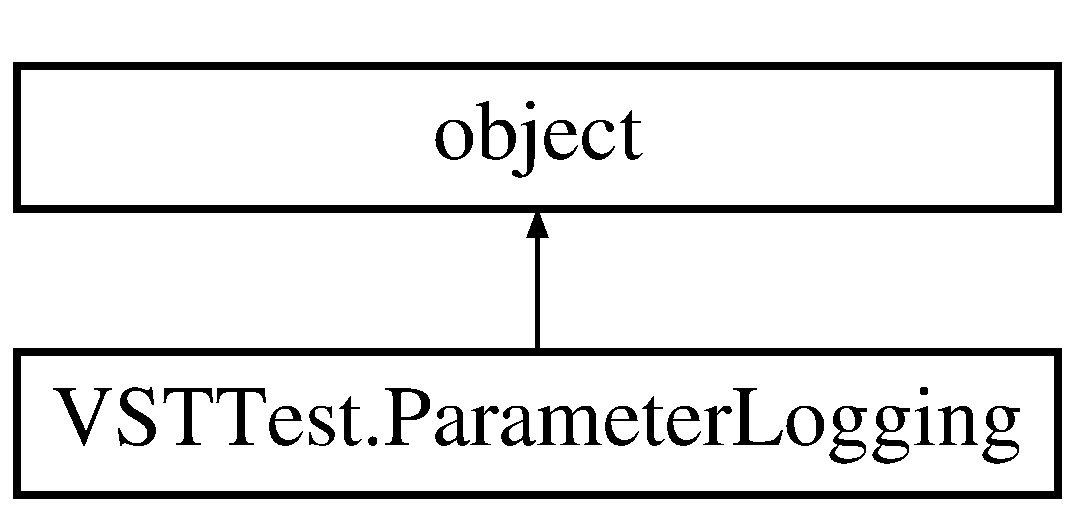
\includegraphics[height=2.000000cm]{class_v_s_t_test_1_1_parameter_logging}
\end{center}
\end{figure}
\subsection*{Public Member Functions}
\begin{DoxyCompactItemize}
\item 
def \hyperlink{class_v_s_t_test_1_1_parameter_logging_ae02d44f336ca02c746c26bd2aa9d74a6}{\+\_\+\+\_\+init\+\_\+\+\_\+} (self, values\+To\+Read, delay=5, fn\+Test=None, backup=0)
\begin{DoxyCompactList}\small\item\em Initializes the test. \end{DoxyCompactList}\item 
def \hyperlink{class_v_s_t_test_1_1_parameter_logging_af6152877e9e239669400dd2a21eed2c9}{run\+Test} (self)
\begin{DoxyCompactList}\small\item\em Starts the logging in a separate thread, moves to the next test. \end{DoxyCompactList}\item 
def \hyperlink{class_v_s_t_test_1_1_parameter_logging_a26fd0345d2477966a108b8c85982c6f0}{stop\+Test} (self)
\begin{DoxyCompactList}\small\item\em Sets the recording option to false, allowing the test to stop. \end{DoxyCompactList}\item 
def \hyperlink{class_v_s_t_test_1_1_parameter_logging_a5018eeef89e877937b38781ff2a5f4ce}{record\+Continuously} (self)
\begin{DoxyCompactList}\small\item\em Continuously records the requested parameters while self.\+recording is set to true. \end{DoxyCompactList}\item 
def \hyperlink{class_v_s_t_test_1_1_parameter_logging_ac4293918415e8732a40b71710f674ec1}{pass\+Fail} (self)
\begin{DoxyCompactList}\small\item\em Determine if the value logging passed -\/ this is done in a separate function, unlike other tests. \end{DoxyCompactList}\item 
def \hyperlink{class_v_s_t_test_1_1_parameter_logging_a2008267f3408fcf63e9cab90f38c5d09}{report} (self, pdf, report\+Path)
\begin{DoxyCompactList}\small\item\em generate this test\textquotesingle{}s page in the P\+DF report. \end{DoxyCompactList}\end{DoxyCompactItemize}


\subsection{Detailed Description}
Periodically records specified values over the course of the testing sequence. 



\subsection{Constructor \& Destructor Documentation}
\index{V\+S\+T\+Test\+::\+Parameter\+Logging@{V\+S\+T\+Test\+::\+Parameter\+Logging}!\+\_\+\+\_\+init\+\_\+\+\_\+@{\+\_\+\+\_\+init\+\_\+\+\_\+}}
\index{\+\_\+\+\_\+init\+\_\+\+\_\+@{\+\_\+\+\_\+init\+\_\+\+\_\+}!V\+S\+T\+Test\+::\+Parameter\+Logging@{V\+S\+T\+Test\+::\+Parameter\+Logging}}
\subsubsection[{\texorpdfstring{\+\_\+\+\_\+init\+\_\+\+\_\+(self, values\+To\+Read, delay=5, fn\+Test=\+None, backup=0)}{__init__(self, valuesToRead, delay=5, fnTest=None, backup=0)}}]{\setlength{\rightskip}{0pt plus 5cm}def V\+S\+T\+Test.\+Parameter\+Logging.\+\_\+\+\_\+init\+\_\+\+\_\+ (
\begin{DoxyParamCaption}
\item[{}]{self, }
\item[{}]{values\+To\+Read, }
\item[{}]{delay = {\ttfamily 5}, }
\item[{}]{fn\+Test = {\ttfamily None}, }
\item[{}]{backup = {\ttfamily 0}}
\end{DoxyParamCaption}
)}\hypertarget{class_v_s_t_test_1_1_parameter_logging_ae02d44f336ca02c746c26bd2aa9d74a6}{}\label{class_v_s_t_test_1_1_parameter_logging_ae02d44f336ca02c746c26bd2aa9d74a6}


Initializes the test. 


\begin{DoxyParams}{Parameters}
{\em values\+To\+Read} & A list of (\char`\"{}subsystem\char`\"{}, \char`\"{}value to read\char`\"{}) tuples \\
\hline
{\em delay} & Time to sleep between periodic queries \\
\hline
{\em fn\+Test} & The Functional\+Test() object, allowing this test to track progress/terminate \\
\hline
{\em backup} & Backup data every n cycles. If zero, do not back up. \\
\hline
\end{DoxyParams}


\subsection{Member Function Documentation}
\index{V\+S\+T\+Test\+::\+Parameter\+Logging@{V\+S\+T\+Test\+::\+Parameter\+Logging}!pass\+Fail@{pass\+Fail}}
\index{pass\+Fail@{pass\+Fail}!V\+S\+T\+Test\+::\+Parameter\+Logging@{V\+S\+T\+Test\+::\+Parameter\+Logging}}
\subsubsection[{\texorpdfstring{pass\+Fail(self)}{passFail(self)}}]{\setlength{\rightskip}{0pt plus 5cm}def V\+S\+T\+Test.\+Parameter\+Logging.\+pass\+Fail (
\begin{DoxyParamCaption}
\item[{}]{self}
\end{DoxyParamCaption}
)}\hypertarget{class_v_s_t_test_1_1_parameter_logging_ac4293918415e8732a40b71710f674ec1}{}\label{class_v_s_t_test_1_1_parameter_logging_ac4293918415e8732a40b71710f674ec1}


Determine if the value logging passed -\/ this is done in a separate function, unlike other tests. 

\index{V\+S\+T\+Test\+::\+Parameter\+Logging@{V\+S\+T\+Test\+::\+Parameter\+Logging}!record\+Continuously@{record\+Continuously}}
\index{record\+Continuously@{record\+Continuously}!V\+S\+T\+Test\+::\+Parameter\+Logging@{V\+S\+T\+Test\+::\+Parameter\+Logging}}
\subsubsection[{\texorpdfstring{record\+Continuously(self)}{recordContinuously(self)}}]{\setlength{\rightskip}{0pt plus 5cm}def V\+S\+T\+Test.\+Parameter\+Logging.\+record\+Continuously (
\begin{DoxyParamCaption}
\item[{}]{self}
\end{DoxyParamCaption}
)}\hypertarget{class_v_s_t_test_1_1_parameter_logging_a5018eeef89e877937b38781ff2a5f4ce}{}\label{class_v_s_t_test_1_1_parameter_logging_a5018eeef89e877937b38781ff2a5f4ce}


Continuously records the requested parameters while self.\+recording is set to true. 

\index{V\+S\+T\+Test\+::\+Parameter\+Logging@{V\+S\+T\+Test\+::\+Parameter\+Logging}!report@{report}}
\index{report@{report}!V\+S\+T\+Test\+::\+Parameter\+Logging@{V\+S\+T\+Test\+::\+Parameter\+Logging}}
\subsubsection[{\texorpdfstring{report(self, pdf, report\+Path)}{report(self, pdf, reportPath)}}]{\setlength{\rightskip}{0pt plus 5cm}def V\+S\+T\+Test.\+Parameter\+Logging.\+report (
\begin{DoxyParamCaption}
\item[{}]{self, }
\item[{}]{pdf, }
\item[{}]{report\+Path}
\end{DoxyParamCaption}
)}\hypertarget{class_v_s_t_test_1_1_parameter_logging_a2008267f3408fcf63e9cab90f38c5d09}{}\label{class_v_s_t_test_1_1_parameter_logging_a2008267f3408fcf63e9cab90f38c5d09}


generate this test\textquotesingle{}s page in the P\+DF report. 


\begin{DoxyParams}{Parameters}
{\em pdf} & pyfpdf-\/compatible P\+DF object. \\
\hline
{\em report\+Path} & Path of directory containing the pdf report \\
\hline
\end{DoxyParams}
\index{V\+S\+T\+Test\+::\+Parameter\+Logging@{V\+S\+T\+Test\+::\+Parameter\+Logging}!run\+Test@{run\+Test}}
\index{run\+Test@{run\+Test}!V\+S\+T\+Test\+::\+Parameter\+Logging@{V\+S\+T\+Test\+::\+Parameter\+Logging}}
\subsubsection[{\texorpdfstring{run\+Test(self)}{runTest(self)}}]{\setlength{\rightskip}{0pt plus 5cm}def V\+S\+T\+Test.\+Parameter\+Logging.\+run\+Test (
\begin{DoxyParamCaption}
\item[{}]{self}
\end{DoxyParamCaption}
)}\hypertarget{class_v_s_t_test_1_1_parameter_logging_af6152877e9e239669400dd2a21eed2c9}{}\label{class_v_s_t_test_1_1_parameter_logging_af6152877e9e239669400dd2a21eed2c9}


Starts the logging in a separate thread, moves to the next test. 

\index{V\+S\+T\+Test\+::\+Parameter\+Logging@{V\+S\+T\+Test\+::\+Parameter\+Logging}!stop\+Test@{stop\+Test}}
\index{stop\+Test@{stop\+Test}!V\+S\+T\+Test\+::\+Parameter\+Logging@{V\+S\+T\+Test\+::\+Parameter\+Logging}}
\subsubsection[{\texorpdfstring{stop\+Test(self)}{stopTest(self)}}]{\setlength{\rightskip}{0pt plus 5cm}def V\+S\+T\+Test.\+Parameter\+Logging.\+stop\+Test (
\begin{DoxyParamCaption}
\item[{}]{self}
\end{DoxyParamCaption}
)}\hypertarget{class_v_s_t_test_1_1_parameter_logging_a26fd0345d2477966a108b8c85982c6f0}{}\label{class_v_s_t_test_1_1_parameter_logging_a26fd0345d2477966a108b8c85982c6f0}


Sets the recording option to false, allowing the test to stop. 



The documentation for this class was generated from the following file\+:\begin{DoxyCompactItemize}
\item 
\hyperlink{_v_s_t_test_8py}{V\+S\+T\+Test.\+py}\end{DoxyCompactItemize}

\hypertarget{class_w_r_e_b_test_1_1_parameter_logging}{}\section{W\+R\+E\+B\+Test.\+Parameter\+Logging Class Reference}
\label{class_w_r_e_b_test_1_1_parameter_logging}\index{W\+R\+E\+B\+Test.\+Parameter\+Logging@{W\+R\+E\+B\+Test.\+Parameter\+Logging}}


Periodically records specified values over the course of the testing sequence.  


Inheritance diagram for W\+R\+E\+B\+Test.\+Parameter\+Logging\+:\begin{figure}[H]
\begin{center}
\leavevmode
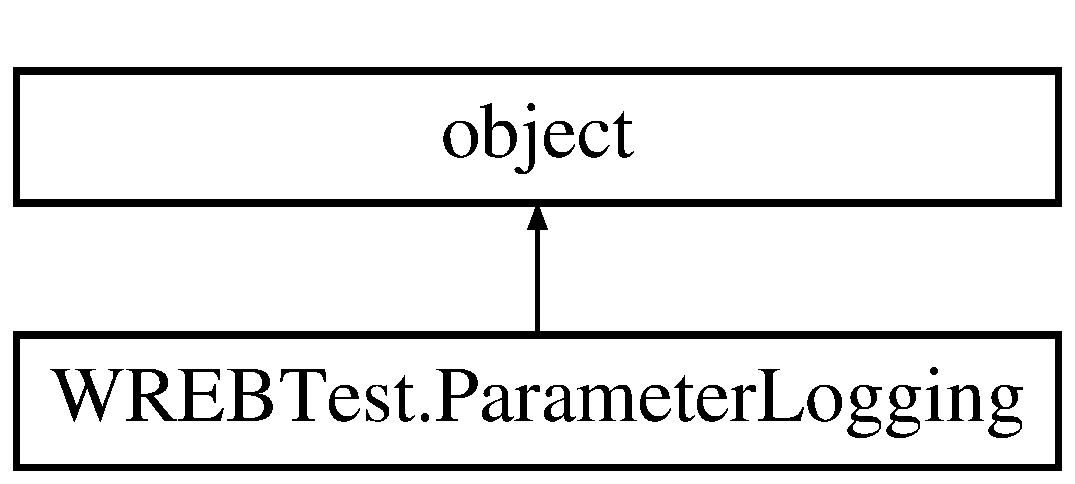
\includegraphics[height=2.000000cm]{class_w_r_e_b_test_1_1_parameter_logging}
\end{center}
\end{figure}
\subsection*{Public Member Functions}
\begin{DoxyCompactItemize}
\item 
def \hyperlink{class_w_r_e_b_test_1_1_parameter_logging_a62abe06e526e6f1a895e46b334e24384}{\+\_\+\+\_\+init\+\_\+\+\_\+} (self, values\+To\+Read, delay=5, fn\+Test=None, backup=0)
\begin{DoxyCompactList}\small\item\em Initializes the test. \end{DoxyCompactList}\item 
def \hyperlink{class_w_r_e_b_test_1_1_parameter_logging_a18edbbadfabec10acb606442bd29d3a6}{run\+Test} (self)
\begin{DoxyCompactList}\small\item\em Starts the logging in a separate thread, moves to the next test. \end{DoxyCompactList}\item 
def \hyperlink{class_w_r_e_b_test_1_1_parameter_logging_af1ed1619ecfea9adf279c4e202aa85c5}{stop\+Test} (self)
\begin{DoxyCompactList}\small\item\em Sets the recording option to false, allowing the test to stop. \end{DoxyCompactList}\item 
def \hyperlink{class_w_r_e_b_test_1_1_parameter_logging_ad8f5c5ee47ced7f956dec174384fb23a}{record\+Continuously} (self)
\begin{DoxyCompactList}\small\item\em Continuously records the requested parameters while self.\+recording is set to true. \end{DoxyCompactList}\item 
def \hyperlink{class_w_r_e_b_test_1_1_parameter_logging_af3556eb776a8a50c983b9b0804228a54}{pass\+Fail} (self)
\begin{DoxyCompactList}\small\item\em Determine if the value logging passed -\/ this is done in a separate function, unlike other tests. \end{DoxyCompactList}\item 
def \hyperlink{class_w_r_e_b_test_1_1_parameter_logging_aa94da9a0cc1c13e48c10e1b4bffc2a26}{report} (self, pdf, report\+Path)
\begin{DoxyCompactList}\small\item\em generate this test\textquotesingle{}s page in the P\+DF report. \end{DoxyCompactList}\end{DoxyCompactItemize}


\subsection{Detailed Description}
Periodically records specified values over the course of the testing sequence. 



\subsection{Constructor \& Destructor Documentation}
\index{W\+R\+E\+B\+Test\+::\+Parameter\+Logging@{W\+R\+E\+B\+Test\+::\+Parameter\+Logging}!\+\_\+\+\_\+init\+\_\+\+\_\+@{\+\_\+\+\_\+init\+\_\+\+\_\+}}
\index{\+\_\+\+\_\+init\+\_\+\+\_\+@{\+\_\+\+\_\+init\+\_\+\+\_\+}!W\+R\+E\+B\+Test\+::\+Parameter\+Logging@{W\+R\+E\+B\+Test\+::\+Parameter\+Logging}}
\subsubsection[{\texorpdfstring{\+\_\+\+\_\+init\+\_\+\+\_\+(self, values\+To\+Read, delay=5, fn\+Test=\+None, backup=0)}{__init__(self, valuesToRead, delay=5, fnTest=None, backup=0)}}]{\setlength{\rightskip}{0pt plus 5cm}def W\+R\+E\+B\+Test.\+Parameter\+Logging.\+\_\+\+\_\+init\+\_\+\+\_\+ (
\begin{DoxyParamCaption}
\item[{}]{self, }
\item[{}]{values\+To\+Read, }
\item[{}]{delay = {\ttfamily 5}, }
\item[{}]{fn\+Test = {\ttfamily None}, }
\item[{}]{backup = {\ttfamily 0}}
\end{DoxyParamCaption}
)}\hypertarget{class_w_r_e_b_test_1_1_parameter_logging_a62abe06e526e6f1a895e46b334e24384}{}\label{class_w_r_e_b_test_1_1_parameter_logging_a62abe06e526e6f1a895e46b334e24384}


Initializes the test. 


\begin{DoxyParams}{Parameters}
{\em values\+To\+Read} & A list of (\char`\"{}subsystem\char`\"{}, \char`\"{}value to read\char`\"{}) tuples \\
\hline
{\em delay} & Time to sleep between periodic queries \\
\hline
{\em fn\+Test} & The Functional\+Test() object, allowing this test to track progress/terminate \\
\hline
{\em backup} & Backup data every n cycles. If zero, do not back up. \\
\hline
\end{DoxyParams}


\subsection{Member Function Documentation}
\index{W\+R\+E\+B\+Test\+::\+Parameter\+Logging@{W\+R\+E\+B\+Test\+::\+Parameter\+Logging}!pass\+Fail@{pass\+Fail}}
\index{pass\+Fail@{pass\+Fail}!W\+R\+E\+B\+Test\+::\+Parameter\+Logging@{W\+R\+E\+B\+Test\+::\+Parameter\+Logging}}
\subsubsection[{\texorpdfstring{pass\+Fail(self)}{passFail(self)}}]{\setlength{\rightskip}{0pt plus 5cm}def W\+R\+E\+B\+Test.\+Parameter\+Logging.\+pass\+Fail (
\begin{DoxyParamCaption}
\item[{}]{self}
\end{DoxyParamCaption}
)}\hypertarget{class_w_r_e_b_test_1_1_parameter_logging_af3556eb776a8a50c983b9b0804228a54}{}\label{class_w_r_e_b_test_1_1_parameter_logging_af3556eb776a8a50c983b9b0804228a54}


Determine if the value logging passed -\/ this is done in a separate function, unlike other tests. 

\index{W\+R\+E\+B\+Test\+::\+Parameter\+Logging@{W\+R\+E\+B\+Test\+::\+Parameter\+Logging}!record\+Continuously@{record\+Continuously}}
\index{record\+Continuously@{record\+Continuously}!W\+R\+E\+B\+Test\+::\+Parameter\+Logging@{W\+R\+E\+B\+Test\+::\+Parameter\+Logging}}
\subsubsection[{\texorpdfstring{record\+Continuously(self)}{recordContinuously(self)}}]{\setlength{\rightskip}{0pt plus 5cm}def W\+R\+E\+B\+Test.\+Parameter\+Logging.\+record\+Continuously (
\begin{DoxyParamCaption}
\item[{}]{self}
\end{DoxyParamCaption}
)}\hypertarget{class_w_r_e_b_test_1_1_parameter_logging_ad8f5c5ee47ced7f956dec174384fb23a}{}\label{class_w_r_e_b_test_1_1_parameter_logging_ad8f5c5ee47ced7f956dec174384fb23a}


Continuously records the requested parameters while self.\+recording is set to true. 

\index{W\+R\+E\+B\+Test\+::\+Parameter\+Logging@{W\+R\+E\+B\+Test\+::\+Parameter\+Logging}!report@{report}}
\index{report@{report}!W\+R\+E\+B\+Test\+::\+Parameter\+Logging@{W\+R\+E\+B\+Test\+::\+Parameter\+Logging}}
\subsubsection[{\texorpdfstring{report(self, pdf, report\+Path)}{report(self, pdf, reportPath)}}]{\setlength{\rightskip}{0pt plus 5cm}def W\+R\+E\+B\+Test.\+Parameter\+Logging.\+report (
\begin{DoxyParamCaption}
\item[{}]{self, }
\item[{}]{pdf, }
\item[{}]{report\+Path}
\end{DoxyParamCaption}
)}\hypertarget{class_w_r_e_b_test_1_1_parameter_logging_aa94da9a0cc1c13e48c10e1b4bffc2a26}{}\label{class_w_r_e_b_test_1_1_parameter_logging_aa94da9a0cc1c13e48c10e1b4bffc2a26}


generate this test\textquotesingle{}s page in the P\+DF report. 


\begin{DoxyParams}{Parameters}
{\em pdf} & pyfpdf-\/compatible P\+DF object. \\
\hline
{\em report\+Path} & Path of directory containing the pdf report \\
\hline
\end{DoxyParams}
\index{W\+R\+E\+B\+Test\+::\+Parameter\+Logging@{W\+R\+E\+B\+Test\+::\+Parameter\+Logging}!run\+Test@{run\+Test}}
\index{run\+Test@{run\+Test}!W\+R\+E\+B\+Test\+::\+Parameter\+Logging@{W\+R\+E\+B\+Test\+::\+Parameter\+Logging}}
\subsubsection[{\texorpdfstring{run\+Test(self)}{runTest(self)}}]{\setlength{\rightskip}{0pt plus 5cm}def W\+R\+E\+B\+Test.\+Parameter\+Logging.\+run\+Test (
\begin{DoxyParamCaption}
\item[{}]{self}
\end{DoxyParamCaption}
)}\hypertarget{class_w_r_e_b_test_1_1_parameter_logging_a18edbbadfabec10acb606442bd29d3a6}{}\label{class_w_r_e_b_test_1_1_parameter_logging_a18edbbadfabec10acb606442bd29d3a6}


Starts the logging in a separate thread, moves to the next test. 

\index{W\+R\+E\+B\+Test\+::\+Parameter\+Logging@{W\+R\+E\+B\+Test\+::\+Parameter\+Logging}!stop\+Test@{stop\+Test}}
\index{stop\+Test@{stop\+Test}!W\+R\+E\+B\+Test\+::\+Parameter\+Logging@{W\+R\+E\+B\+Test\+::\+Parameter\+Logging}}
\subsubsection[{\texorpdfstring{stop\+Test(self)}{stopTest(self)}}]{\setlength{\rightskip}{0pt plus 5cm}def W\+R\+E\+B\+Test.\+Parameter\+Logging.\+stop\+Test (
\begin{DoxyParamCaption}
\item[{}]{self}
\end{DoxyParamCaption}
)}\hypertarget{class_w_r_e_b_test_1_1_parameter_logging_af1ed1619ecfea9adf279c4e202aa85c5}{}\label{class_w_r_e_b_test_1_1_parameter_logging_af1ed1619ecfea9adf279c4e202aa85c5}


Sets the recording option to false, allowing the test to stop. 



The documentation for this class was generated from the following file\+:\begin{DoxyCompactItemize}
\item 
\hyperlink{_w_r_e_b_test_8py}{W\+R\+E\+B\+Test.\+py}\end{DoxyCompactItemize}

\hypertarget{class_g_r_e_b_test_1_1_p_c_k_rails}{}\section{G\+R\+E\+B\+Test.\+P\+C\+K\+Rails Class Reference}
\label{class_g_r_e_b_test_1_1_p_c_k_rails}\index{G\+R\+E\+B\+Test.\+P\+C\+K\+Rails@{G\+R\+E\+B\+Test.\+P\+C\+K\+Rails}}


Tests the parallel clock rail performance.  


Inheritance diagram for G\+R\+E\+B\+Test.\+P\+C\+K\+Rails\+:\begin{figure}[H]
\begin{center}
\leavevmode
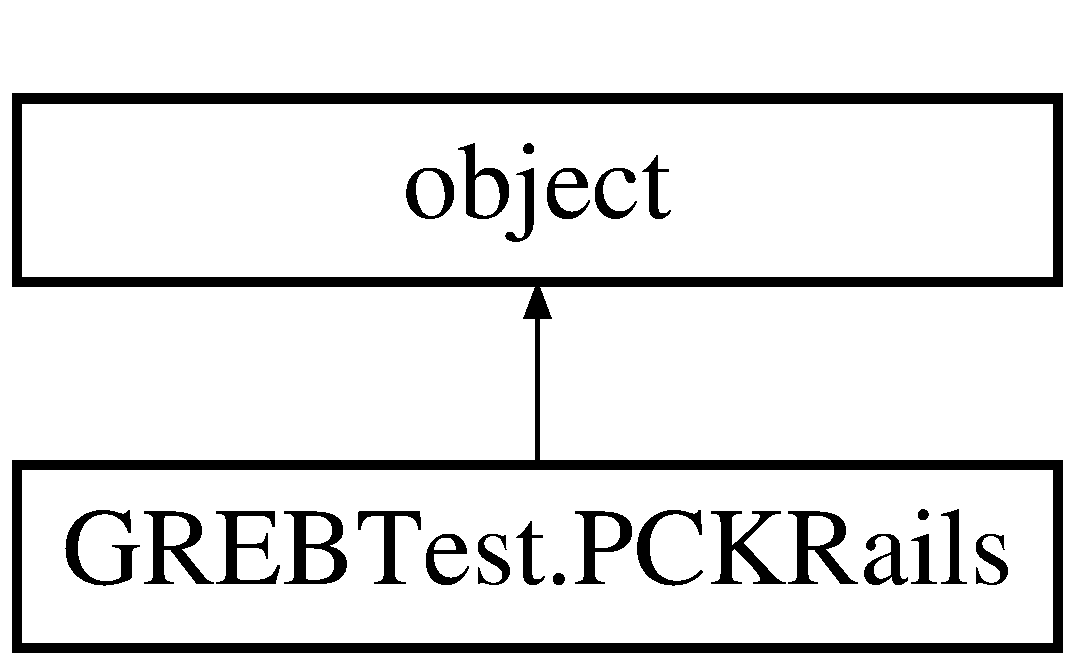
\includegraphics[height=2.000000cm]{class_g_r_e_b_test_1_1_p_c_k_rails}
\end{center}
\end{figure}
\subsection*{Public Member Functions}
\begin{DoxyCompactItemize}
\item 
def \hyperlink{class_g_r_e_b_test_1_1_p_c_k_rails_a00b31975b5faca18c8be81b21b0ba741}{\+\_\+\+\_\+init\+\_\+\+\_\+} (self)
\begin{DoxyCompactList}\small\item\em Initialize minimum required variables for test list. \end{DoxyCompactList}\item 
def \hyperlink{class_g_r_e_b_test_1_1_p_c_k_rails_a88eadd5557a36e319f6b45924573c741}{run\+Test} (self)
\begin{DoxyCompactList}\small\item\em Run the test, save output to state variables. \end{DoxyCompactList}\item 
def \hyperlink{class_g_r_e_b_test_1_1_p_c_k_rails_a277a4fe1cbbd534b76206edd189e89a2}{summarize} (self, summary)
\begin{DoxyCompactList}\small\item\em Summarize the test results for the cover page of the report. \end{DoxyCompactList}\item 
def \hyperlink{class_g_r_e_b_test_1_1_p_c_k_rails_ae1f03dd0cd9709f339fecd9004be7843}{report} (self, pdf, report\+Path)
\begin{DoxyCompactList}\small\item\em generate this test\textquotesingle{}s page in the P\+DF report. \end{DoxyCompactList}\end{DoxyCompactItemize}


\subsection{Detailed Description}
Tests the parallel clock rail performance. 



\subsection{Constructor \& Destructor Documentation}
\index{G\+R\+E\+B\+Test\+::\+P\+C\+K\+Rails@{G\+R\+E\+B\+Test\+::\+P\+C\+K\+Rails}!\+\_\+\+\_\+init\+\_\+\+\_\+@{\+\_\+\+\_\+init\+\_\+\+\_\+}}
\index{\+\_\+\+\_\+init\+\_\+\+\_\+@{\+\_\+\+\_\+init\+\_\+\+\_\+}!G\+R\+E\+B\+Test\+::\+P\+C\+K\+Rails@{G\+R\+E\+B\+Test\+::\+P\+C\+K\+Rails}}
\subsubsection[{\texorpdfstring{\+\_\+\+\_\+init\+\_\+\+\_\+(self)}{__init__(self)}}]{\setlength{\rightskip}{0pt plus 5cm}def G\+R\+E\+B\+Test.\+P\+C\+K\+Rails.\+\_\+\+\_\+init\+\_\+\+\_\+ (
\begin{DoxyParamCaption}
\item[{}]{self}
\end{DoxyParamCaption}
)}\hypertarget{class_g_r_e_b_test_1_1_p_c_k_rails_a00b31975b5faca18c8be81b21b0ba741}{}\label{class_g_r_e_b_test_1_1_p_c_k_rails_a00b31975b5faca18c8be81b21b0ba741}


Initialize minimum required variables for test list. 



\subsection{Member Function Documentation}
\index{G\+R\+E\+B\+Test\+::\+P\+C\+K\+Rails@{G\+R\+E\+B\+Test\+::\+P\+C\+K\+Rails}!report@{report}}
\index{report@{report}!G\+R\+E\+B\+Test\+::\+P\+C\+K\+Rails@{G\+R\+E\+B\+Test\+::\+P\+C\+K\+Rails}}
\subsubsection[{\texorpdfstring{report(self, pdf, report\+Path)}{report(self, pdf, reportPath)}}]{\setlength{\rightskip}{0pt plus 5cm}def G\+R\+E\+B\+Test.\+P\+C\+K\+Rails.\+report (
\begin{DoxyParamCaption}
\item[{}]{self, }
\item[{}]{pdf, }
\item[{}]{report\+Path}
\end{DoxyParamCaption}
)}\hypertarget{class_g_r_e_b_test_1_1_p_c_k_rails_ae1f03dd0cd9709f339fecd9004be7843}{}\label{class_g_r_e_b_test_1_1_p_c_k_rails_ae1f03dd0cd9709f339fecd9004be7843}


generate this test\textquotesingle{}s page in the P\+DF report. 


\begin{DoxyParams}{Parameters}
{\em pdf} & pyfpdf-\/compatible P\+DF object. \\
\hline
{\em report\+Path} & Path of directory containing the pdf report \\
\hline
\end{DoxyParams}
\index{G\+R\+E\+B\+Test\+::\+P\+C\+K\+Rails@{G\+R\+E\+B\+Test\+::\+P\+C\+K\+Rails}!run\+Test@{run\+Test}}
\index{run\+Test@{run\+Test}!G\+R\+E\+B\+Test\+::\+P\+C\+K\+Rails@{G\+R\+E\+B\+Test\+::\+P\+C\+K\+Rails}}
\subsubsection[{\texorpdfstring{run\+Test(self)}{runTest(self)}}]{\setlength{\rightskip}{0pt plus 5cm}def G\+R\+E\+B\+Test.\+P\+C\+K\+Rails.\+run\+Test (
\begin{DoxyParamCaption}
\item[{}]{self}
\end{DoxyParamCaption}
)}\hypertarget{class_g_r_e_b_test_1_1_p_c_k_rails_a88eadd5557a36e319f6b45924573c741}{}\label{class_g_r_e_b_test_1_1_p_c_k_rails_a88eadd5557a36e319f6b45924573c741}


Run the test, save output to state variables. 

\index{G\+R\+E\+B\+Test\+::\+P\+C\+K\+Rails@{G\+R\+E\+B\+Test\+::\+P\+C\+K\+Rails}!summarize@{summarize}}
\index{summarize@{summarize}!G\+R\+E\+B\+Test\+::\+P\+C\+K\+Rails@{G\+R\+E\+B\+Test\+::\+P\+C\+K\+Rails}}
\subsubsection[{\texorpdfstring{summarize(self, summary)}{summarize(self, summary)}}]{\setlength{\rightskip}{0pt plus 5cm}def G\+R\+E\+B\+Test.\+P\+C\+K\+Rails.\+summarize (
\begin{DoxyParamCaption}
\item[{}]{self, }
\item[{}]{summary}
\end{DoxyParamCaption}
)}\hypertarget{class_g_r_e_b_test_1_1_p_c_k_rails_a277a4fe1cbbd534b76206edd189e89a2}{}\label{class_g_r_e_b_test_1_1_p_c_k_rails_a277a4fe1cbbd534b76206edd189e89a2}


Summarize the test results for the cover page of the report. 


\begin{DoxyParams}{Parameters}
{\em summary} & \hyperlink{class_g_r_e_b_test_1_1_summary}{Summary} obejct passed from Functional\+Test() \\
\hline
\end{DoxyParams}


The documentation for this class was generated from the following file\+:\begin{DoxyCompactItemize}
\item 
\hyperlink{_g_r_e_b_test_8py}{G\+R\+E\+B\+Test.\+py}\end{DoxyCompactItemize}

\hypertarget{class_w_r_e_b_test_1_1_p_c_k_rails}{}\section{W\+R\+E\+B\+Test.\+P\+C\+K\+Rails Class Reference}
\label{class_w_r_e_b_test_1_1_p_c_k_rails}\index{W\+R\+E\+B\+Test.\+P\+C\+K\+Rails@{W\+R\+E\+B\+Test.\+P\+C\+K\+Rails}}


Test the parallel clock rail performance.  


Inheritance diagram for W\+R\+E\+B\+Test.\+P\+C\+K\+Rails\+:\begin{figure}[H]
\begin{center}
\leavevmode
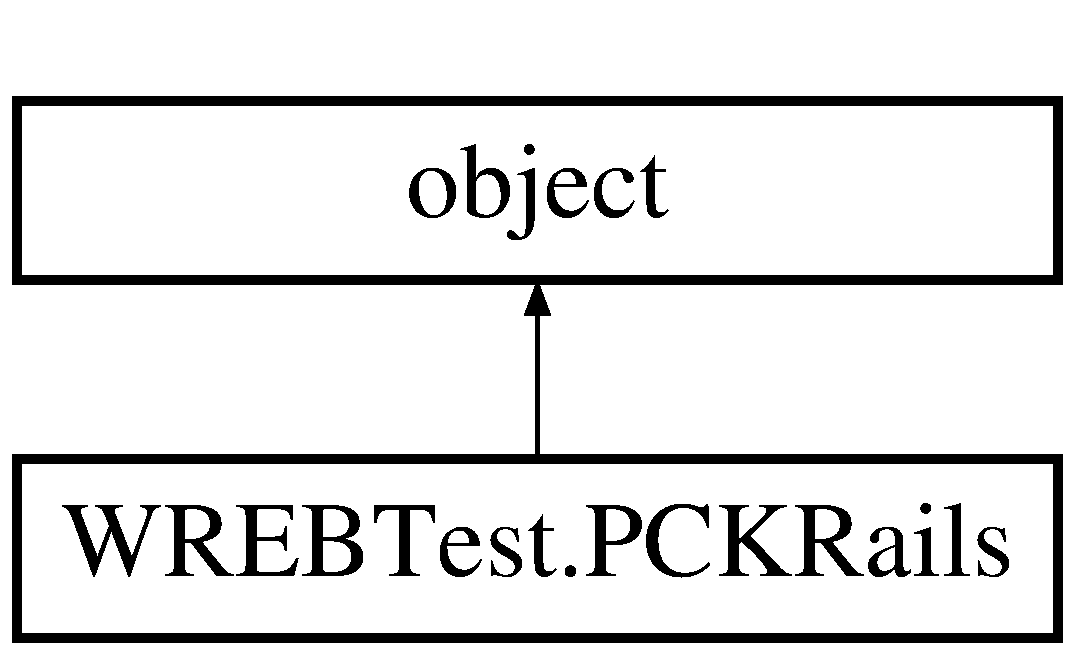
\includegraphics[height=2.000000cm]{class_w_r_e_b_test_1_1_p_c_k_rails}
\end{center}
\end{figure}
\subsection*{Public Member Functions}
\begin{DoxyCompactItemize}
\item 
def \hyperlink{class_w_r_e_b_test_1_1_p_c_k_rails_a09480a5ceddb45da89954585ca9a8d7b}{\+\_\+\+\_\+init\+\_\+\+\_\+} (self)
\begin{DoxyCompactList}\small\item\em Initialize minimum required variables for test list. \end{DoxyCompactList}\item 
def \hyperlink{class_w_r_e_b_test_1_1_p_c_k_rails_a5e706f60ff883d7222b185e082ea7182}{run\+Test} (self)
\begin{DoxyCompactList}\small\item\em Run the test, save output to state variables. \end{DoxyCompactList}\item 
def \hyperlink{class_w_r_e_b_test_1_1_p_c_k_rails_a905d8777dfc5419eca9975e0318cc0ea}{summarize} (self, summary)
\begin{DoxyCompactList}\small\item\em Summarize the test results for the cover page of the report. \end{DoxyCompactList}\item 
def \hyperlink{class_w_r_e_b_test_1_1_p_c_k_rails_ab37489050c10320ee091de8aadfd68a7}{report} (self, pdf)
\begin{DoxyCompactList}\small\item\em generate this test\textquotesingle{}s page in the P\+DF report. \end{DoxyCompactList}\end{DoxyCompactItemize}


\subsection{Detailed Description}
Test the parallel clock rail performance. 



\subsection{Constructor \& Destructor Documentation}
\index{W\+R\+E\+B\+Test\+::\+P\+C\+K\+Rails@{W\+R\+E\+B\+Test\+::\+P\+C\+K\+Rails}!\+\_\+\+\_\+init\+\_\+\+\_\+@{\+\_\+\+\_\+init\+\_\+\+\_\+}}
\index{\+\_\+\+\_\+init\+\_\+\+\_\+@{\+\_\+\+\_\+init\+\_\+\+\_\+}!W\+R\+E\+B\+Test\+::\+P\+C\+K\+Rails@{W\+R\+E\+B\+Test\+::\+P\+C\+K\+Rails}}
\subsubsection[{\texorpdfstring{\+\_\+\+\_\+init\+\_\+\+\_\+(self)}{__init__(self)}}]{\setlength{\rightskip}{0pt plus 5cm}def W\+R\+E\+B\+Test.\+P\+C\+K\+Rails.\+\_\+\+\_\+init\+\_\+\+\_\+ (
\begin{DoxyParamCaption}
\item[{}]{self}
\end{DoxyParamCaption}
)}\hypertarget{class_w_r_e_b_test_1_1_p_c_k_rails_a09480a5ceddb45da89954585ca9a8d7b}{}\label{class_w_r_e_b_test_1_1_p_c_k_rails_a09480a5ceddb45da89954585ca9a8d7b}


Initialize minimum required variables for test list. 



\subsection{Member Function Documentation}
\index{W\+R\+E\+B\+Test\+::\+P\+C\+K\+Rails@{W\+R\+E\+B\+Test\+::\+P\+C\+K\+Rails}!report@{report}}
\index{report@{report}!W\+R\+E\+B\+Test\+::\+P\+C\+K\+Rails@{W\+R\+E\+B\+Test\+::\+P\+C\+K\+Rails}}
\subsubsection[{\texorpdfstring{report(self, pdf)}{report(self, pdf)}}]{\setlength{\rightskip}{0pt plus 5cm}def W\+R\+E\+B\+Test.\+P\+C\+K\+Rails.\+report (
\begin{DoxyParamCaption}
\item[{}]{self, }
\item[{}]{pdf}
\end{DoxyParamCaption}
)}\hypertarget{class_w_r_e_b_test_1_1_p_c_k_rails_ab37489050c10320ee091de8aadfd68a7}{}\label{class_w_r_e_b_test_1_1_p_c_k_rails_ab37489050c10320ee091de8aadfd68a7}


generate this test\textquotesingle{}s page in the P\+DF report. 


\begin{DoxyParams}{Parameters}
{\em pdf} & pyfpdf-\/compatible P\+DF object. \\
\hline
\end{DoxyParams}
\index{W\+R\+E\+B\+Test\+::\+P\+C\+K\+Rails@{W\+R\+E\+B\+Test\+::\+P\+C\+K\+Rails}!run\+Test@{run\+Test}}
\index{run\+Test@{run\+Test}!W\+R\+E\+B\+Test\+::\+P\+C\+K\+Rails@{W\+R\+E\+B\+Test\+::\+P\+C\+K\+Rails}}
\subsubsection[{\texorpdfstring{run\+Test(self)}{runTest(self)}}]{\setlength{\rightskip}{0pt plus 5cm}def W\+R\+E\+B\+Test.\+P\+C\+K\+Rails.\+run\+Test (
\begin{DoxyParamCaption}
\item[{}]{self}
\end{DoxyParamCaption}
)}\hypertarget{class_w_r_e_b_test_1_1_p_c_k_rails_a5e706f60ff883d7222b185e082ea7182}{}\label{class_w_r_e_b_test_1_1_p_c_k_rails_a5e706f60ff883d7222b185e082ea7182}


Run the test, save output to state variables. 

\index{W\+R\+E\+B\+Test\+::\+P\+C\+K\+Rails@{W\+R\+E\+B\+Test\+::\+P\+C\+K\+Rails}!summarize@{summarize}}
\index{summarize@{summarize}!W\+R\+E\+B\+Test\+::\+P\+C\+K\+Rails@{W\+R\+E\+B\+Test\+::\+P\+C\+K\+Rails}}
\subsubsection[{\texorpdfstring{summarize(self, summary)}{summarize(self, summary)}}]{\setlength{\rightskip}{0pt plus 5cm}def W\+R\+E\+B\+Test.\+P\+C\+K\+Rails.\+summarize (
\begin{DoxyParamCaption}
\item[{}]{self, }
\item[{}]{summary}
\end{DoxyParamCaption}
)}\hypertarget{class_w_r_e_b_test_1_1_p_c_k_rails_a905d8777dfc5419eca9975e0318cc0ea}{}\label{class_w_r_e_b_test_1_1_p_c_k_rails_a905d8777dfc5419eca9975e0318cc0ea}


Summarize the test results for the cover page of the report. 


\begin{DoxyParams}{Parameters}
{\em summary} & \hyperlink{class_w_r_e_b_test_1_1_summary}{Summary} obejct passed from Functional\+Test() \\
\hline
\end{DoxyParams}


The documentation for this class was generated from the following file\+:\begin{DoxyCompactItemize}
\item 
\hyperlink{_w_r_e_b_test_8py}{W\+R\+E\+B\+Test.\+py}\end{DoxyCompactItemize}

\hypertarget{class_v_s_t_test_1_1_p_c_k_rails}{}\section{V\+S\+T\+Test.\+P\+C\+K\+Rails Class Reference}
\label{class_v_s_t_test_1_1_p_c_k_rails}\index{V\+S\+T\+Test.\+P\+C\+K\+Rails@{V\+S\+T\+Test.\+P\+C\+K\+Rails}}


Tests the parallel clock rail performance.  


Inheritance diagram for V\+S\+T\+Test.\+P\+C\+K\+Rails\+:\begin{figure}[H]
\begin{center}
\leavevmode
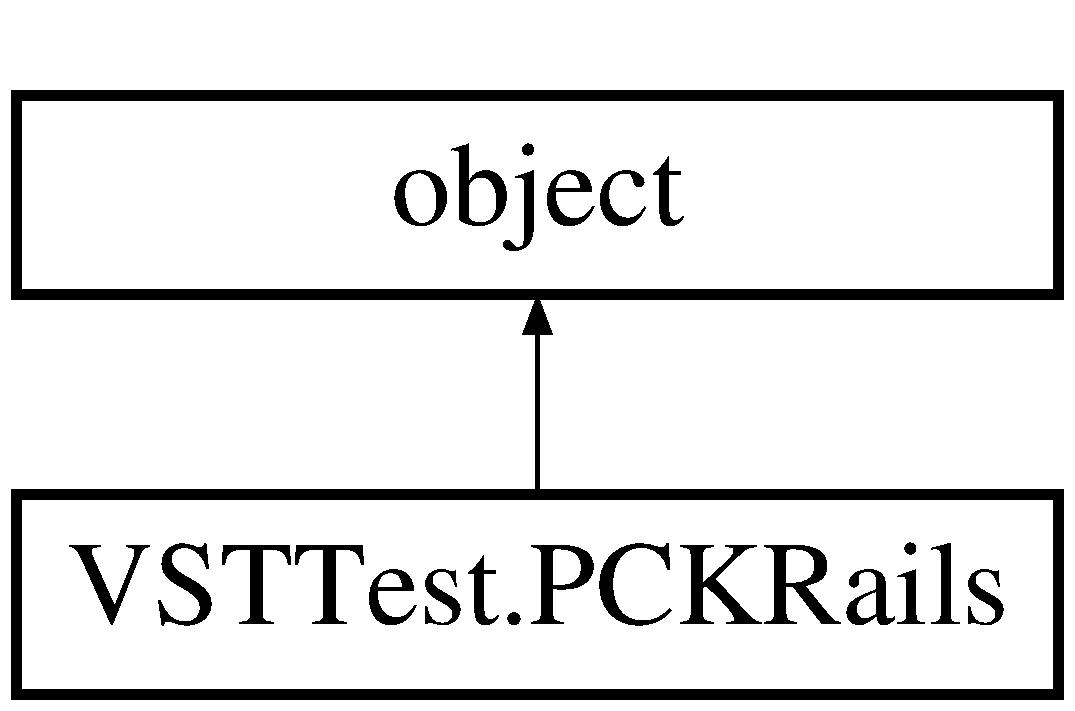
\includegraphics[height=2.000000cm]{class_v_s_t_test_1_1_p_c_k_rails}
\end{center}
\end{figure}
\subsection*{Public Member Functions}
\begin{DoxyCompactItemize}
\item 
def \hyperlink{class_v_s_t_test_1_1_p_c_k_rails_a4987db68048645a88d3bcf997b2dd025}{\+\_\+\+\_\+init\+\_\+\+\_\+} (self)
\begin{DoxyCompactList}\small\item\em Initialize minimum required variables for test list. \end{DoxyCompactList}\item 
def \hyperlink{class_v_s_t_test_1_1_p_c_k_rails_a9f2e2cb16e1fc652bf616bda7a61b35b}{run\+Test} (self)
\begin{DoxyCompactList}\small\item\em Run the test, save output to state variables. \end{DoxyCompactList}\item 
def \hyperlink{class_v_s_t_test_1_1_p_c_k_rails_a848e1924e7e16672cea96152ba852387}{summarize} (self, summary)
\begin{DoxyCompactList}\small\item\em Summarize the test results for the cover page of the report. \end{DoxyCompactList}\item 
def \hyperlink{class_v_s_t_test_1_1_p_c_k_rails_a9cda7cc2d2094acd84397e4ace3a34e9}{report} (self, pdf, report\+Path)
\begin{DoxyCompactList}\small\item\em generate this test\textquotesingle{}s page in the P\+DF report. \end{DoxyCompactList}\end{DoxyCompactItemize}


\subsection{Detailed Description}
Tests the parallel clock rail performance. 



\subsection{Constructor \& Destructor Documentation}
\index{V\+S\+T\+Test\+::\+P\+C\+K\+Rails@{V\+S\+T\+Test\+::\+P\+C\+K\+Rails}!\+\_\+\+\_\+init\+\_\+\+\_\+@{\+\_\+\+\_\+init\+\_\+\+\_\+}}
\index{\+\_\+\+\_\+init\+\_\+\+\_\+@{\+\_\+\+\_\+init\+\_\+\+\_\+}!V\+S\+T\+Test\+::\+P\+C\+K\+Rails@{V\+S\+T\+Test\+::\+P\+C\+K\+Rails}}
\subsubsection[{\texorpdfstring{\+\_\+\+\_\+init\+\_\+\+\_\+(self)}{__init__(self)}}]{\setlength{\rightskip}{0pt plus 5cm}def V\+S\+T\+Test.\+P\+C\+K\+Rails.\+\_\+\+\_\+init\+\_\+\+\_\+ (
\begin{DoxyParamCaption}
\item[{}]{self}
\end{DoxyParamCaption}
)}\hypertarget{class_v_s_t_test_1_1_p_c_k_rails_a4987db68048645a88d3bcf997b2dd025}{}\label{class_v_s_t_test_1_1_p_c_k_rails_a4987db68048645a88d3bcf997b2dd025}


Initialize minimum required variables for test list. 



\subsection{Member Function Documentation}
\index{V\+S\+T\+Test\+::\+P\+C\+K\+Rails@{V\+S\+T\+Test\+::\+P\+C\+K\+Rails}!report@{report}}
\index{report@{report}!V\+S\+T\+Test\+::\+P\+C\+K\+Rails@{V\+S\+T\+Test\+::\+P\+C\+K\+Rails}}
\subsubsection[{\texorpdfstring{report(self, pdf, report\+Path)}{report(self, pdf, reportPath)}}]{\setlength{\rightskip}{0pt plus 5cm}def V\+S\+T\+Test.\+P\+C\+K\+Rails.\+report (
\begin{DoxyParamCaption}
\item[{}]{self, }
\item[{}]{pdf, }
\item[{}]{report\+Path}
\end{DoxyParamCaption}
)}\hypertarget{class_v_s_t_test_1_1_p_c_k_rails_a9cda7cc2d2094acd84397e4ace3a34e9}{}\label{class_v_s_t_test_1_1_p_c_k_rails_a9cda7cc2d2094acd84397e4ace3a34e9}


generate this test\textquotesingle{}s page in the P\+DF report. 


\begin{DoxyParams}{Parameters}
{\em pdf} & pyfpdf-\/compatible P\+DF object. \\
\hline
{\em report\+Path} & Path of directory containing the pdf report \\
\hline
\end{DoxyParams}
\index{V\+S\+T\+Test\+::\+P\+C\+K\+Rails@{V\+S\+T\+Test\+::\+P\+C\+K\+Rails}!run\+Test@{run\+Test}}
\index{run\+Test@{run\+Test}!V\+S\+T\+Test\+::\+P\+C\+K\+Rails@{V\+S\+T\+Test\+::\+P\+C\+K\+Rails}}
\subsubsection[{\texorpdfstring{run\+Test(self)}{runTest(self)}}]{\setlength{\rightskip}{0pt plus 5cm}def V\+S\+T\+Test.\+P\+C\+K\+Rails.\+run\+Test (
\begin{DoxyParamCaption}
\item[{}]{self}
\end{DoxyParamCaption}
)}\hypertarget{class_v_s_t_test_1_1_p_c_k_rails_a9f2e2cb16e1fc652bf616bda7a61b35b}{}\label{class_v_s_t_test_1_1_p_c_k_rails_a9f2e2cb16e1fc652bf616bda7a61b35b}


Run the test, save output to state variables. 

\index{V\+S\+T\+Test\+::\+P\+C\+K\+Rails@{V\+S\+T\+Test\+::\+P\+C\+K\+Rails}!summarize@{summarize}}
\index{summarize@{summarize}!V\+S\+T\+Test\+::\+P\+C\+K\+Rails@{V\+S\+T\+Test\+::\+P\+C\+K\+Rails}}
\subsubsection[{\texorpdfstring{summarize(self, summary)}{summarize(self, summary)}}]{\setlength{\rightskip}{0pt plus 5cm}def V\+S\+T\+Test.\+P\+C\+K\+Rails.\+summarize (
\begin{DoxyParamCaption}
\item[{}]{self, }
\item[{}]{summary}
\end{DoxyParamCaption}
)}\hypertarget{class_v_s_t_test_1_1_p_c_k_rails_a848e1924e7e16672cea96152ba852387}{}\label{class_v_s_t_test_1_1_p_c_k_rails_a848e1924e7e16672cea96152ba852387}


Summarize the test results for the cover page of the report. 


\begin{DoxyParams}{Parameters}
{\em summary} & \hyperlink{class_v_s_t_test_1_1_summary}{Summary} obejct passed from Functional\+Test() \\
\hline
\end{DoxyParams}


The documentation for this class was generated from the following file\+:\begin{DoxyCompactItemize}
\item 
\hyperlink{_v_s_t_test_8py}{V\+S\+T\+Test.\+py}\end{DoxyCompactItemize}

\hypertarget{classpdf_gen_w_r_e_b_1_1_p_d_f}{}\section{pdf\+Gen\+W\+R\+E\+B.\+P\+DF Class Reference}
\label{classpdf_gen_w_r_e_b_1_1_p_d_f}\index{pdf\+Gen\+W\+R\+E\+B.\+P\+DF@{pdf\+Gen\+W\+R\+E\+B.\+P\+DF}}


\hyperlink{classpdf_gen_w_r_e_b_1_1_p_d_f}{P\+DF} generation class for reports.  


Inheritance diagram for pdf\+Gen\+W\+R\+E\+B.\+P\+DF\+:\begin{figure}[H]
\begin{center}
\leavevmode
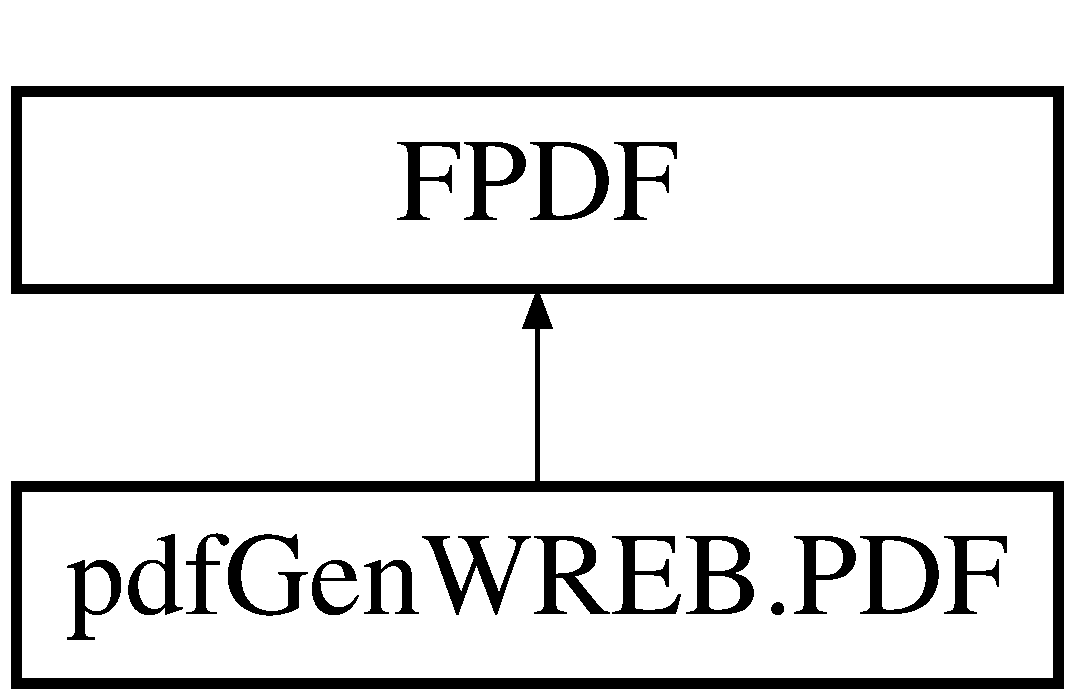
\includegraphics[height=2.000000cm]{classpdf_gen_w_r_e_b_1_1_p_d_f}
\end{center}
\end{figure}
\subsection*{Public Member Functions}
\begin{DoxyCompactItemize}
\item 
def \hyperlink{classpdf_gen_w_r_e_b_1_1_p_d_f_ae0da62a475a1b97d62428ae3c662f2a6}{header} (self)
\begin{DoxyCompactList}\small\item\em Adds a L\+S\+S\+T/\+S\+L\+AC header and title to every page. \end{DoxyCompactList}\item 
def \hyperlink{classpdf_gen_w_r_e_b_1_1_p_d_f_a01a4153716448dc03856712735fee900}{footer} (self)
\begin{DoxyCompactList}\small\item\em Adds page numbers to every page. \end{DoxyCompactList}\item 
def \hyperlink{classpdf_gen_w_r_e_b_1_1_p_d_f_a682682f02997f0cc3fefc7468265a90b}{test\+Title} (self, title)
\begin{DoxyCompactList}\small\item\em Generic title function for tests. \end{DoxyCompactList}\item 
def \hyperlink{classpdf_gen_w_r_e_b_1_1_p_d_f_a08028486631686cbf99a23e97485478b}{summary\+Page} (self, board\+ID, board\+Type, link\+Version, F\+P\+G\+A\+Version, script\+Version, start\+Time, test\+List, pass\+List, stats\+List)
\begin{DoxyCompactList}\small\item\em Generate a summary page for the tests that were run. \end{DoxyCompactList}\item 
def \hyperlink{classpdf_gen_w_r_e_b_1_1_p_d_f_a38eb7da8869e7b9252f9e6dad3d5129b}{column\+Table} (self, col\+Data, R\+OI=None, col\+Headers=None, font\+Size=8, width=1.\+0, width\+Array=None, align=\char`\"{}L\char`\"{})
\begin{DoxyCompactList}\small\item\em Generates a table from a list of lists of column data. \end{DoxyCompactList}\item 
def \hyperlink{classpdf_gen_w_r_e_b_1_1_p_d_f_ab9270daacb7fb78b62b040fb389a1a3f}{add\+Plot\+Page} (self, title, img\+Name, img\+Size=1.\+0)
\begin{DoxyCompactList}\small\item\em Adds a page for tests with outputs consisting only of an image/plot. \end{DoxyCompactList}\item 
def \hyperlink{classpdf_gen_w_r_e_b_1_1_p_d_f_a0c03db1c6bbb6d9de9fec314cf845cbb}{idle\+Current} (self, title, voltages, currents)
\begin{DoxyCompactList}\small\item\em Idle current generation test, will be moved to \hyperlink{_w_r_e_b_test_8py}{W\+R\+E\+B\+Test.\+py} soon. \end{DoxyCompactList}\item 
def \hyperlink{classpdf_gen_w_r_e_b_1_1_p_d_f_ae508c11aef02aa49d0e846a03b71abf2}{residual\+Test} (self, title, datas, residuals, passed, stats, R\+OI=None, img\+Size=0.\+7, xdat=None, plt\+Range=None)
\begin{DoxyCompactList}\small\item\em Report page for tests that consist of a single residual plot, including comments and pass/fail. \end{DoxyCompactList}\item 
def \hyperlink{classpdf_gen_w_r_e_b_1_1_p_d_f_a6fa66ac0799cc7bd37698f30f0136931}{make\+Residual\+Plot\+Page} (self, title, img\+Name, datas, residuals, R\+OI=None, img\+Size=1.\+0, xdat=None, plt\+Range=None)
\begin{DoxyCompactList}\small\item\em Generates the new page and plot for the residual tests. \end{DoxyCompactList}\item 
def \hyperlink{classpdf_gen_w_r_e_b_1_1_p_d_f_a6d5d3b21e55356e95a2c73d2e086620c}{make\+Plot\+Page} (self, title, img\+Name, datas, img\+Size=1.\+0, xdat=None)
\begin{DoxyCompactList}\small\item\em Generates the new page and plot for the non-\/residual tests. \end{DoxyCompactList}\item 
def \hyperlink{classpdf_gen_w_r_e_b_1_1_p_d_f_ab247acf933388e099f79ae0213f72972}{pass\+Fail} (self, passed)
\begin{DoxyCompactList}\small\item\em Return color-\/coded pass/fail result. \end{DoxyCompactList}\end{DoxyCompactItemize}


\subsection{Detailed Description}
\hyperlink{classpdf_gen_w_r_e_b_1_1_p_d_f}{P\+DF} generation class for reports. 

\subsection{Member Function Documentation}
\index{pdf\+Gen\+W\+R\+E\+B\+::\+P\+DF@{pdf\+Gen\+W\+R\+E\+B\+::\+P\+DF}!add\+Plot\+Page@{add\+Plot\+Page}}
\index{add\+Plot\+Page@{add\+Plot\+Page}!pdf\+Gen\+W\+R\+E\+B\+::\+P\+DF@{pdf\+Gen\+W\+R\+E\+B\+::\+P\+DF}}
\subsubsection[{\texorpdfstring{add\+Plot\+Page(self, title, img\+Name, img\+Size=1.\+0)}{addPlotPage(self, title, imgName, imgSize=1.0)}}]{\setlength{\rightskip}{0pt plus 5cm}def pdf\+Gen\+W\+R\+E\+B.\+P\+D\+F.\+add\+Plot\+Page (
\begin{DoxyParamCaption}
\item[{}]{self, }
\item[{}]{title, }
\item[{}]{img\+Name, }
\item[{}]{img\+Size = {\ttfamily 1.0}}
\end{DoxyParamCaption}
)}\hypertarget{classpdf_gen_w_r_e_b_1_1_p_d_f_ab9270daacb7fb78b62b040fb389a1a3f}{}\label{classpdf_gen_w_r_e_b_1_1_p_d_f_ab9270daacb7fb78b62b040fb389a1a3f}


Adds a page for tests with outputs consisting only of an image/plot. 


\begin{DoxyParams}{Parameters}
{\em title} & Title of test on page \\
\hline
{\em img\+Name} & File to save plot as \\
\hline
{\em img\+Size} & Optional, percent of page width image should take up; defaults to 1.\+0 \\
\hline
\end{DoxyParams}
\index{pdf\+Gen\+W\+R\+E\+B\+::\+P\+DF@{pdf\+Gen\+W\+R\+E\+B\+::\+P\+DF}!column\+Table@{column\+Table}}
\index{column\+Table@{column\+Table}!pdf\+Gen\+W\+R\+E\+B\+::\+P\+DF@{pdf\+Gen\+W\+R\+E\+B\+::\+P\+DF}}
\subsubsection[{\texorpdfstring{column\+Table(self, col\+Data, R\+O\+I=\+None, col\+Headers=\+None, font\+Size=8, width=1.\+0, width\+Array=\+None, align=""L"")}{columnTable(self, colData, ROI=None, colHeaders=None, fontSize=8, width=1.0, widthArray=None, align="L")}}]{\setlength{\rightskip}{0pt plus 5cm}def pdf\+Gen\+W\+R\+E\+B.\+P\+D\+F.\+column\+Table (
\begin{DoxyParamCaption}
\item[{}]{self, }
\item[{}]{col\+Data, }
\item[{}]{R\+OI = {\ttfamily None}, }
\item[{}]{col\+Headers = {\ttfamily None}, }
\item[{}]{font\+Size = {\ttfamily 8}, }
\item[{}]{width = {\ttfamily 1.0}, }
\item[{}]{width\+Array = {\ttfamily None}, }
\item[{}]{align = {\ttfamily \char`\"{}L\char`\"{}}}
\end{DoxyParamCaption}
)}\hypertarget{classpdf_gen_w_r_e_b_1_1_p_d_f_a38eb7da8869e7b9252f9e6dad3d5129b}{}\label{classpdf_gen_w_r_e_b_1_1_p_d_f_a38eb7da8869e7b9252f9e6dad3d5129b}


Generates a table from a list of lists of column data. 


\begin{DoxyParams}{Parameters}
{\em col\+Data} & Tuple of column information as (\mbox{[}data\mbox{]}, header) to be put in a column, from left to right. \\
\hline
{\em R\+OI} & Optional parameter of \mbox{[}low, high\mbox{]} index of cells to be highlighted as a region of interest. \\
\hline
{\em col\+Headers} & Optional list of headers for columns; if specified, col\+Data is expected as (\mbox{[}data\mbox{]},\mbox{[}data\mbox{]},...) \\
\hline
{\em font\+Size} & Optional font size for the table. \\
\hline
{\em width} & Percent of page width the table should occupy. \\
\hline
{\em width\+Array} & Non-\/normalized list of relative column widths. Defaults to every column having equal width. \\
\hline
{\em align} & Align as left (\char`\"{}\+L\char`\"{}), center (\char`\"{}\+C\char`\"{}), right (\char`\"{}\+R\char`\"{}) \\
\hline
\end{DoxyParams}
\index{pdf\+Gen\+W\+R\+E\+B\+::\+P\+DF@{pdf\+Gen\+W\+R\+E\+B\+::\+P\+DF}!footer@{footer}}
\index{footer@{footer}!pdf\+Gen\+W\+R\+E\+B\+::\+P\+DF@{pdf\+Gen\+W\+R\+E\+B\+::\+P\+DF}}
\subsubsection[{\texorpdfstring{footer(self)}{footer(self)}}]{\setlength{\rightskip}{0pt plus 5cm}def pdf\+Gen\+W\+R\+E\+B.\+P\+D\+F.\+footer (
\begin{DoxyParamCaption}
\item[{}]{self}
\end{DoxyParamCaption}
)}\hypertarget{classpdf_gen_w_r_e_b_1_1_p_d_f_a01a4153716448dc03856712735fee900}{}\label{classpdf_gen_w_r_e_b_1_1_p_d_f_a01a4153716448dc03856712735fee900}


Adds page numbers to every page. 

\index{pdf\+Gen\+W\+R\+E\+B\+::\+P\+DF@{pdf\+Gen\+W\+R\+E\+B\+::\+P\+DF}!header@{header}}
\index{header@{header}!pdf\+Gen\+W\+R\+E\+B\+::\+P\+DF@{pdf\+Gen\+W\+R\+E\+B\+::\+P\+DF}}
\subsubsection[{\texorpdfstring{header(self)}{header(self)}}]{\setlength{\rightskip}{0pt plus 5cm}def pdf\+Gen\+W\+R\+E\+B.\+P\+D\+F.\+header (
\begin{DoxyParamCaption}
\item[{}]{self}
\end{DoxyParamCaption}
)}\hypertarget{classpdf_gen_w_r_e_b_1_1_p_d_f_ae0da62a475a1b97d62428ae3c662f2a6}{}\label{classpdf_gen_w_r_e_b_1_1_p_d_f_ae0da62a475a1b97d62428ae3c662f2a6}


Adds a L\+S\+S\+T/\+S\+L\+AC header and title to every page. 

\index{pdf\+Gen\+W\+R\+E\+B\+::\+P\+DF@{pdf\+Gen\+W\+R\+E\+B\+::\+P\+DF}!idle\+Current@{idle\+Current}}
\index{idle\+Current@{idle\+Current}!pdf\+Gen\+W\+R\+E\+B\+::\+P\+DF@{pdf\+Gen\+W\+R\+E\+B\+::\+P\+DF}}
\subsubsection[{\texorpdfstring{idle\+Current(self, title, voltages, currents)}{idleCurrent(self, title, voltages, currents)}}]{\setlength{\rightskip}{0pt plus 5cm}def pdf\+Gen\+W\+R\+E\+B.\+P\+D\+F.\+idle\+Current (
\begin{DoxyParamCaption}
\item[{}]{self, }
\item[{}]{title, }
\item[{}]{voltages, }
\item[{}]{currents}
\end{DoxyParamCaption}
)}\hypertarget{classpdf_gen_w_r_e_b_1_1_p_d_f_a0c03db1c6bbb6d9de9fec314cf845cbb}{}\label{classpdf_gen_w_r_e_b_1_1_p_d_f_a0c03db1c6bbb6d9de9fec314cf845cbb}


Idle current generation test, will be moved to \hyperlink{_w_r_e_b_test_8py}{W\+R\+E\+B\+Test.\+py} soon. 


\begin{DoxyParams}{Parameters}
{\em title} & Title of test on page \\
\hline
{\em voltages} & List of (category title, \mbox{[}voltages\mbox{]}) \\
\hline
{\em currents} & List of (category title, \mbox{[}currents\mbox{]}) \\
\hline
\end{DoxyParams}
\index{pdf\+Gen\+W\+R\+E\+B\+::\+P\+DF@{pdf\+Gen\+W\+R\+E\+B\+::\+P\+DF}!make\+Plot\+Page@{make\+Plot\+Page}}
\index{make\+Plot\+Page@{make\+Plot\+Page}!pdf\+Gen\+W\+R\+E\+B\+::\+P\+DF@{pdf\+Gen\+W\+R\+E\+B\+::\+P\+DF}}
\subsubsection[{\texorpdfstring{make\+Plot\+Page(self, title, img\+Name, datas, img\+Size=1.\+0, xdat=\+None)}{makePlotPage(self, title, imgName, datas, imgSize=1.0, xdat=None)}}]{\setlength{\rightskip}{0pt plus 5cm}def pdf\+Gen\+W\+R\+E\+B.\+P\+D\+F.\+make\+Plot\+Page (
\begin{DoxyParamCaption}
\item[{}]{self, }
\item[{}]{title, }
\item[{}]{img\+Name, }
\item[{}]{datas, }
\item[{}]{img\+Size = {\ttfamily 1.0}, }
\item[{}]{xdat = {\ttfamily None}}
\end{DoxyParamCaption}
)}\hypertarget{classpdf_gen_w_r_e_b_1_1_p_d_f_a6d5d3b21e55356e95a2c73d2e086620c}{}\label{classpdf_gen_w_r_e_b_1_1_p_d_f_a6d5d3b21e55356e95a2c73d2e086620c}


Generates the new page and plot for the non-\/residual tests. 


\begin{DoxyParams}{Parameters}
{\em title} & Title of test on page \\
\hline
{\em img\+Name} & Title of temporary plot image \\
\hline
{\em datas} & Zipped data arrays and legend titles \\
\hline
{\em img\+Size} & Optional, percent of page width image should take up; defaults to 1.\+0 \\
\hline
{\em xdat} & Optional zipped array of x values and titles. Defaults to iteration values. \\
\hline
\end{DoxyParams}
\index{pdf\+Gen\+W\+R\+E\+B\+::\+P\+DF@{pdf\+Gen\+W\+R\+E\+B\+::\+P\+DF}!make\+Residual\+Plot\+Page@{make\+Residual\+Plot\+Page}}
\index{make\+Residual\+Plot\+Page@{make\+Residual\+Plot\+Page}!pdf\+Gen\+W\+R\+E\+B\+::\+P\+DF@{pdf\+Gen\+W\+R\+E\+B\+::\+P\+DF}}
\subsubsection[{\texorpdfstring{make\+Residual\+Plot\+Page(self, title, img\+Name, datas, residuals, R\+O\+I=\+None, img\+Size=1.\+0, xdat=\+None, plt\+Range=\+None)}{makeResidualPlotPage(self, title, imgName, datas, residuals, ROI=None, imgSize=1.0, xdat=None, pltRange=None)}}]{\setlength{\rightskip}{0pt plus 5cm}def pdf\+Gen\+W\+R\+E\+B.\+P\+D\+F.\+make\+Residual\+Plot\+Page (
\begin{DoxyParamCaption}
\item[{}]{self, }
\item[{}]{title, }
\item[{}]{img\+Name, }
\item[{}]{datas, }
\item[{}]{residuals, }
\item[{}]{R\+OI = {\ttfamily None}, }
\item[{}]{img\+Size = {\ttfamily 1.0}, }
\item[{}]{xdat = {\ttfamily None}, }
\item[{}]{plt\+Range = {\ttfamily None}}
\end{DoxyParamCaption}
)}\hypertarget{classpdf_gen_w_r_e_b_1_1_p_d_f_a6fa66ac0799cc7bd37698f30f0136931}{}\label{classpdf_gen_w_r_e_b_1_1_p_d_f_a6fa66ac0799cc7bd37698f30f0136931}


Generates the new page and plot for the residual tests. 


\begin{DoxyParams}{Parameters}
{\em title} & Title of test on page \\
\hline
{\em img\+Name} & Title of temporary plot image \\
\hline
{\em datas} & Zipped data arrays and legend titles \\
\hline
{\em residuals} & Zipped array of residuals and legend titles \\
\hline
{\em R\+OI} & Optional parameter specifying region of interest in the plot \\
\hline
{\em img\+Size} & Optional, percent of page width image should take up; defaults to 1.\+0 \\
\hline
{\em xdat} & Optional zipped array of x values and titles. Defaults to iteration values. \\
\hline
{\em plt\+Range} & Optional specified plot range. \\
\hline
\end{DoxyParams}
\index{pdf\+Gen\+W\+R\+E\+B\+::\+P\+DF@{pdf\+Gen\+W\+R\+E\+B\+::\+P\+DF}!pass\+Fail@{pass\+Fail}}
\index{pass\+Fail@{pass\+Fail}!pdf\+Gen\+W\+R\+E\+B\+::\+P\+DF@{pdf\+Gen\+W\+R\+E\+B\+::\+P\+DF}}
\subsubsection[{\texorpdfstring{pass\+Fail(self, passed)}{passFail(self, passed)}}]{\setlength{\rightskip}{0pt plus 5cm}def pdf\+Gen\+W\+R\+E\+B.\+P\+D\+F.\+pass\+Fail (
\begin{DoxyParamCaption}
\item[{}]{self, }
\item[{}]{passed}
\end{DoxyParamCaption}
)}\hypertarget{classpdf_gen_w_r_e_b_1_1_p_d_f_ab247acf933388e099f79ae0213f72972}{}\label{classpdf_gen_w_r_e_b_1_1_p_d_f_ab247acf933388e099f79ae0213f72972}


Return color-\/coded pass/fail result. 


\begin{DoxyParams}{Parameters}
{\em passed} & String of either \char`\"{}\+P\+A\+S\+S\char`\"{} or \char`\"{}\+F\+A\+I\+L\char`\"{} \\
\hline
\end{DoxyParams}
\index{pdf\+Gen\+W\+R\+E\+B\+::\+P\+DF@{pdf\+Gen\+W\+R\+E\+B\+::\+P\+DF}!residual\+Test@{residual\+Test}}
\index{residual\+Test@{residual\+Test}!pdf\+Gen\+W\+R\+E\+B\+::\+P\+DF@{pdf\+Gen\+W\+R\+E\+B\+::\+P\+DF}}
\subsubsection[{\texorpdfstring{residual\+Test(self, title, datas, residuals, passed, stats, R\+O\+I=\+None, img\+Size=0.\+7, xdat=\+None, plt\+Range=\+None)}{residualTest(self, title, datas, residuals, passed, stats, ROI=None, imgSize=0.7, xdat=None, pltRange=None)}}]{\setlength{\rightskip}{0pt plus 5cm}def pdf\+Gen\+W\+R\+E\+B.\+P\+D\+F.\+residual\+Test (
\begin{DoxyParamCaption}
\item[{}]{self, }
\item[{}]{title, }
\item[{}]{datas, }
\item[{}]{residuals, }
\item[{}]{passed, }
\item[{}]{stats, }
\item[{}]{R\+OI = {\ttfamily None}, }
\item[{}]{img\+Size = {\ttfamily 0.7}, }
\item[{}]{xdat = {\ttfamily None}, }
\item[{}]{plt\+Range = {\ttfamily None}}
\end{DoxyParamCaption}
)}\hypertarget{classpdf_gen_w_r_e_b_1_1_p_d_f_ae508c11aef02aa49d0e846a03b71abf2}{}\label{classpdf_gen_w_r_e_b_1_1_p_d_f_ae508c11aef02aa49d0e846a03b71abf2}


Report page for tests that consist of a single residual plot, including comments and pass/fail. 


\begin{DoxyParams}{Parameters}
{\em title} & Title of test on page and title of temporary plot image \\
\hline
{\em datas} & Zipped data arrays and legend titles \\
\hline
{\em residuals} & Zipped array of residuals and legend titles \\
\hline
{\em passed} & Pass/fail result of test \\
\hline
{\em stats} & Relevant comments from the test \\
\hline
{\em R\+OI} & Optional parameter specifying region of interest in the plot \\
\hline
{\em img\+Size} & Optional, percent of page width image should take up; defaults to 1.\+0 \\
\hline
{\em xdat} & Optional zipped array of x values and titles. Defaults to iteration values. \\
\hline
{\em plt\+Range} & Optional specified plot range. \\
\hline
\end{DoxyParams}
\index{pdf\+Gen\+W\+R\+E\+B\+::\+P\+DF@{pdf\+Gen\+W\+R\+E\+B\+::\+P\+DF}!summary\+Page@{summary\+Page}}
\index{summary\+Page@{summary\+Page}!pdf\+Gen\+W\+R\+E\+B\+::\+P\+DF@{pdf\+Gen\+W\+R\+E\+B\+::\+P\+DF}}
\subsubsection[{\texorpdfstring{summary\+Page(self, board\+I\+D, board\+Type, link\+Version, F\+P\+G\+A\+Version, script\+Version, start\+Time, test\+List, pass\+List, stats\+List)}{summaryPage(self, boardID, boardType, linkVersion, FPGAVersion, scriptVersion, startTime, testList, passList, statsList)}}]{\setlength{\rightskip}{0pt plus 5cm}def pdf\+Gen\+W\+R\+E\+B.\+P\+D\+F.\+summary\+Page (
\begin{DoxyParamCaption}
\item[{}]{self, }
\item[{}]{board\+ID, }
\item[{}]{board\+Type, }
\item[{}]{link\+Version, }
\item[{}]{F\+P\+G\+A\+Version, }
\item[{}]{script\+Version, }
\item[{}]{start\+Time, }
\item[{}]{test\+List, }
\item[{}]{pass\+List, }
\item[{}]{stats\+List}
\end{DoxyParamCaption}
)}\hypertarget{classpdf_gen_w_r_e_b_1_1_p_d_f_a08028486631686cbf99a23e97485478b}{}\label{classpdf_gen_w_r_e_b_1_1_p_d_f_a08028486631686cbf99a23e97485478b}


Generate a summary page for the tests that were run. 


\begin{DoxyParams}{Parameters}
{\em board\+ID} & Serial number of the board that is tested \\
\hline
{\em board\+Type} & Type of phsyical board model \\
\hline
{\em link\+Version} & Version of link software \\
\hline
{\em F\+P\+G\+A\+Version} & Front-\/end F\+P\+GA code version \\
\hline
{\em script\+Version} & Version of the script, given by the last modified date Y\+Y.\+M\+M.\+D\+D.\+hh.\+mm.\+ss \\
\hline
{\em test\+List} & List of test titles that were run \\
\hline
{\em pass\+List} & List of test results \\
\hline
{\em stats\+List} & List of relevant statistics returned from the tests \\
\hline
\end{DoxyParams}
\index{pdf\+Gen\+W\+R\+E\+B\+::\+P\+DF@{pdf\+Gen\+W\+R\+E\+B\+::\+P\+DF}!test\+Title@{test\+Title}}
\index{test\+Title@{test\+Title}!pdf\+Gen\+W\+R\+E\+B\+::\+P\+DF@{pdf\+Gen\+W\+R\+E\+B\+::\+P\+DF}}
\subsubsection[{\texorpdfstring{test\+Title(self, title)}{testTitle(self, title)}}]{\setlength{\rightskip}{0pt plus 5cm}def pdf\+Gen\+W\+R\+E\+B.\+P\+D\+F.\+test\+Title (
\begin{DoxyParamCaption}
\item[{}]{self, }
\item[{}]{title}
\end{DoxyParamCaption}
)}\hypertarget{classpdf_gen_w_r_e_b_1_1_p_d_f_a682682f02997f0cc3fefc7468265a90b}{}\label{classpdf_gen_w_r_e_b_1_1_p_d_f_a682682f02997f0cc3fefc7468265a90b}


Generic title function for tests. 



The documentation for this class was generated from the following file\+:\begin{DoxyCompactItemize}
\item 
\hyperlink{pdf_gen_w_r_e_b_8py}{pdf\+Gen\+W\+R\+E\+B.\+py}\end{DoxyCompactItemize}

\hypertarget{class_g_r_e_b_test_1_1_r_d_bias}{}\section{G\+R\+E\+B\+Test.\+R\+D\+Bias Class Reference}
\label{class_g_r_e_b_test_1_1_r_d_bias}\index{G\+R\+E\+B\+Test.\+R\+D\+Bias@{G\+R\+E\+B\+Test.\+R\+D\+Bias}}


Tests the reset drain performance.  


Inheritance diagram for G\+R\+E\+B\+Test.\+R\+D\+Bias\+:\begin{figure}[H]
\begin{center}
\leavevmode
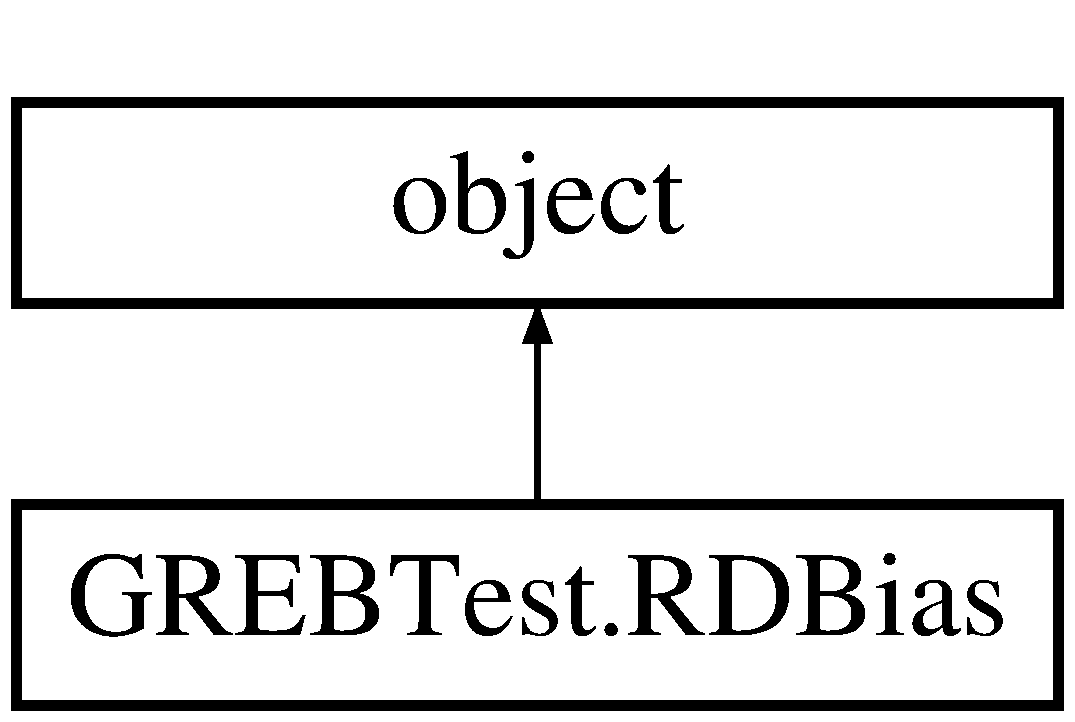
\includegraphics[height=2.000000cm]{class_g_r_e_b_test_1_1_r_d_bias}
\end{center}
\end{figure}
\subsection*{Public Member Functions}
\begin{DoxyCompactItemize}
\item 
def \hyperlink{class_g_r_e_b_test_1_1_r_d_bias_a03fa3204f1b14c82c6aab46eff1dfc6d}{\+\_\+\+\_\+init\+\_\+\+\_\+} (self)
\begin{DoxyCompactList}\small\item\em Initialize minimum required variables for test list. \end{DoxyCompactList}\item 
def \hyperlink{class_g_r_e_b_test_1_1_r_d_bias_a5c88a3421501fa0f0875a9fb0fc7f8db}{run\+Test} (self)
\begin{DoxyCompactList}\small\item\em Run the test, save output to state variables. \end{DoxyCompactList}\item 
def \hyperlink{class_g_r_e_b_test_1_1_r_d_bias_aa6e369baa9f067780f6588cbf6161470}{summarize} (self, summary)
\begin{DoxyCompactList}\small\item\em Summarize the test results for the cover page of the report. \end{DoxyCompactList}\item 
def \hyperlink{class_g_r_e_b_test_1_1_r_d_bias_ae10f981e67f5b0f8a7f016e28b006866}{report} (self, pdf, report\+Path)
\begin{DoxyCompactList}\small\item\em generate this test\textquotesingle{}s page in the P\+DF report. \end{DoxyCompactList}\end{DoxyCompactItemize}


\subsection{Detailed Description}
Tests the reset drain performance. 



\subsection{Constructor \& Destructor Documentation}
\index{G\+R\+E\+B\+Test\+::\+R\+D\+Bias@{G\+R\+E\+B\+Test\+::\+R\+D\+Bias}!\+\_\+\+\_\+init\+\_\+\+\_\+@{\+\_\+\+\_\+init\+\_\+\+\_\+}}
\index{\+\_\+\+\_\+init\+\_\+\+\_\+@{\+\_\+\+\_\+init\+\_\+\+\_\+}!G\+R\+E\+B\+Test\+::\+R\+D\+Bias@{G\+R\+E\+B\+Test\+::\+R\+D\+Bias}}
\subsubsection[{\texorpdfstring{\+\_\+\+\_\+init\+\_\+\+\_\+(self)}{__init__(self)}}]{\setlength{\rightskip}{0pt plus 5cm}def G\+R\+E\+B\+Test.\+R\+D\+Bias.\+\_\+\+\_\+init\+\_\+\+\_\+ (
\begin{DoxyParamCaption}
\item[{}]{self}
\end{DoxyParamCaption}
)}\hypertarget{class_g_r_e_b_test_1_1_r_d_bias_a03fa3204f1b14c82c6aab46eff1dfc6d}{}\label{class_g_r_e_b_test_1_1_r_d_bias_a03fa3204f1b14c82c6aab46eff1dfc6d}


Initialize minimum required variables for test list. 



\subsection{Member Function Documentation}
\index{G\+R\+E\+B\+Test\+::\+R\+D\+Bias@{G\+R\+E\+B\+Test\+::\+R\+D\+Bias}!report@{report}}
\index{report@{report}!G\+R\+E\+B\+Test\+::\+R\+D\+Bias@{G\+R\+E\+B\+Test\+::\+R\+D\+Bias}}
\subsubsection[{\texorpdfstring{report(self, pdf, report\+Path)}{report(self, pdf, reportPath)}}]{\setlength{\rightskip}{0pt plus 5cm}def G\+R\+E\+B\+Test.\+R\+D\+Bias.\+report (
\begin{DoxyParamCaption}
\item[{}]{self, }
\item[{}]{pdf, }
\item[{}]{report\+Path}
\end{DoxyParamCaption}
)}\hypertarget{class_g_r_e_b_test_1_1_r_d_bias_ae10f981e67f5b0f8a7f016e28b006866}{}\label{class_g_r_e_b_test_1_1_r_d_bias_ae10f981e67f5b0f8a7f016e28b006866}


generate this test\textquotesingle{}s page in the P\+DF report. 


\begin{DoxyParams}{Parameters}
{\em pdf} & pyfpdf-\/compatible P\+DF object. \\
\hline
{\em report\+Path} & Path of directory containing the pdf report \\
\hline
\end{DoxyParams}
\index{G\+R\+E\+B\+Test\+::\+R\+D\+Bias@{G\+R\+E\+B\+Test\+::\+R\+D\+Bias}!run\+Test@{run\+Test}}
\index{run\+Test@{run\+Test}!G\+R\+E\+B\+Test\+::\+R\+D\+Bias@{G\+R\+E\+B\+Test\+::\+R\+D\+Bias}}
\subsubsection[{\texorpdfstring{run\+Test(self)}{runTest(self)}}]{\setlength{\rightskip}{0pt plus 5cm}def G\+R\+E\+B\+Test.\+R\+D\+Bias.\+run\+Test (
\begin{DoxyParamCaption}
\item[{}]{self}
\end{DoxyParamCaption}
)}\hypertarget{class_g_r_e_b_test_1_1_r_d_bias_a5c88a3421501fa0f0875a9fb0fc7f8db}{}\label{class_g_r_e_b_test_1_1_r_d_bias_a5c88a3421501fa0f0875a9fb0fc7f8db}


Run the test, save output to state variables. 

\index{G\+R\+E\+B\+Test\+::\+R\+D\+Bias@{G\+R\+E\+B\+Test\+::\+R\+D\+Bias}!summarize@{summarize}}
\index{summarize@{summarize}!G\+R\+E\+B\+Test\+::\+R\+D\+Bias@{G\+R\+E\+B\+Test\+::\+R\+D\+Bias}}
\subsubsection[{\texorpdfstring{summarize(self, summary)}{summarize(self, summary)}}]{\setlength{\rightskip}{0pt plus 5cm}def G\+R\+E\+B\+Test.\+R\+D\+Bias.\+summarize (
\begin{DoxyParamCaption}
\item[{}]{self, }
\item[{}]{summary}
\end{DoxyParamCaption}
)}\hypertarget{class_g_r_e_b_test_1_1_r_d_bias_aa6e369baa9f067780f6588cbf6161470}{}\label{class_g_r_e_b_test_1_1_r_d_bias_aa6e369baa9f067780f6588cbf6161470}


Summarize the test results for the cover page of the report. 


\begin{DoxyParams}{Parameters}
{\em summary} & \hyperlink{class_g_r_e_b_test_1_1_summary}{Summary} obejct passed from Functional\+Test() \\
\hline
\end{DoxyParams}


The documentation for this class was generated from the following file\+:\begin{DoxyCompactItemize}
\item 
\hyperlink{_g_r_e_b_test_8py}{G\+R\+E\+B\+Test.\+py}\end{DoxyCompactItemize}

\hypertarget{class_v_s_t_test_1_1_r_d_bias}{}\section{V\+S\+T\+Test.\+R\+D\+Bias Class Reference}
\label{class_v_s_t_test_1_1_r_d_bias}\index{V\+S\+T\+Test.\+R\+D\+Bias@{V\+S\+T\+Test.\+R\+D\+Bias}}


Tests the reset drain performance.  


Inheritance diagram for V\+S\+T\+Test.\+R\+D\+Bias\+:\begin{figure}[H]
\begin{center}
\leavevmode
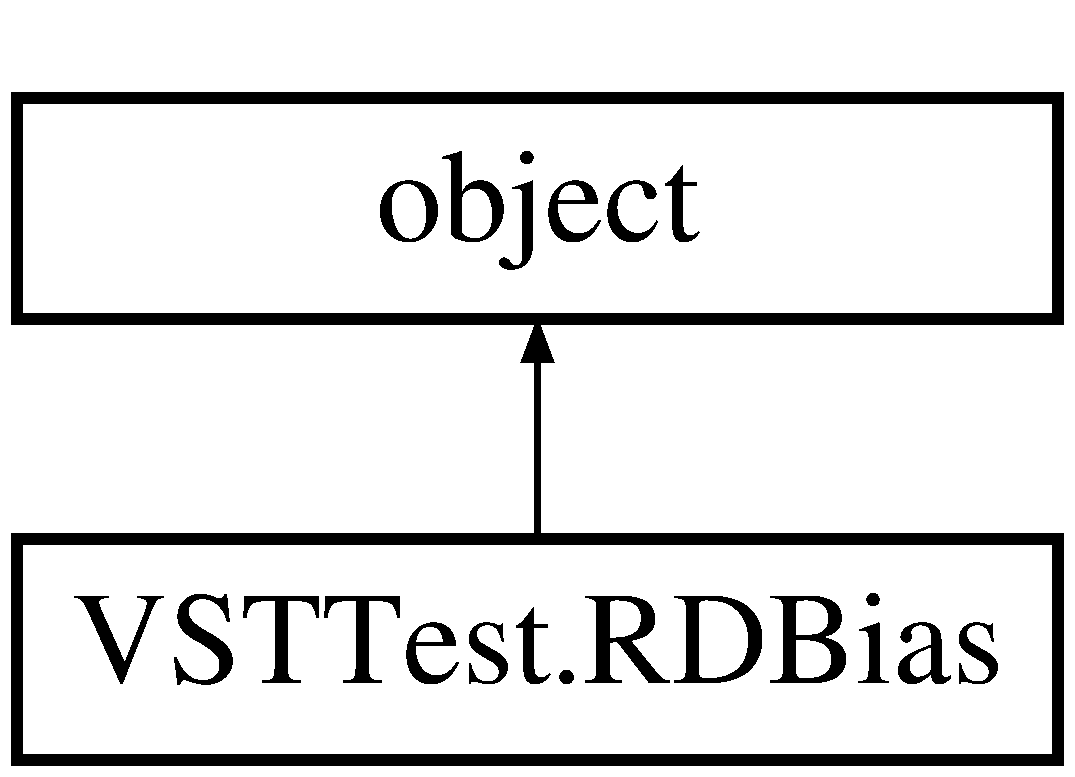
\includegraphics[height=2.000000cm]{class_v_s_t_test_1_1_r_d_bias}
\end{center}
\end{figure}
\subsection*{Public Member Functions}
\begin{DoxyCompactItemize}
\item 
def \hyperlink{class_v_s_t_test_1_1_r_d_bias_a40c667035a3b876fcc79fb2081ed4b56}{\+\_\+\+\_\+init\+\_\+\+\_\+} (self)
\begin{DoxyCompactList}\small\item\em Initialize minimum required variables for test list. \end{DoxyCompactList}\item 
def \hyperlink{class_v_s_t_test_1_1_r_d_bias_a93ed826cc1fdd7c1d850a585419821c7}{run\+Test} (self)
\begin{DoxyCompactList}\small\item\em Run the test, save output to state variables. \end{DoxyCompactList}\item 
def \hyperlink{class_v_s_t_test_1_1_r_d_bias_a2e3395c4c17e6f257193e00de4cadb33}{summarize} (self, summary)
\begin{DoxyCompactList}\small\item\em Summarize the test results for the cover page of the report. \end{DoxyCompactList}\item 
def \hyperlink{class_v_s_t_test_1_1_r_d_bias_ab53a33a86263b30f47c4b2945647f6cc}{report} (self, pdf, report\+Path)
\begin{DoxyCompactList}\small\item\em generate this test\textquotesingle{}s page in the P\+DF report. \end{DoxyCompactList}\end{DoxyCompactItemize}


\subsection{Detailed Description}
Tests the reset drain performance. 



\subsection{Constructor \& Destructor Documentation}
\index{V\+S\+T\+Test\+::\+R\+D\+Bias@{V\+S\+T\+Test\+::\+R\+D\+Bias}!\+\_\+\+\_\+init\+\_\+\+\_\+@{\+\_\+\+\_\+init\+\_\+\+\_\+}}
\index{\+\_\+\+\_\+init\+\_\+\+\_\+@{\+\_\+\+\_\+init\+\_\+\+\_\+}!V\+S\+T\+Test\+::\+R\+D\+Bias@{V\+S\+T\+Test\+::\+R\+D\+Bias}}
\subsubsection[{\texorpdfstring{\+\_\+\+\_\+init\+\_\+\+\_\+(self)}{__init__(self)}}]{\setlength{\rightskip}{0pt plus 5cm}def V\+S\+T\+Test.\+R\+D\+Bias.\+\_\+\+\_\+init\+\_\+\+\_\+ (
\begin{DoxyParamCaption}
\item[{}]{self}
\end{DoxyParamCaption}
)}\hypertarget{class_v_s_t_test_1_1_r_d_bias_a40c667035a3b876fcc79fb2081ed4b56}{}\label{class_v_s_t_test_1_1_r_d_bias_a40c667035a3b876fcc79fb2081ed4b56}


Initialize minimum required variables for test list. 



\subsection{Member Function Documentation}
\index{V\+S\+T\+Test\+::\+R\+D\+Bias@{V\+S\+T\+Test\+::\+R\+D\+Bias}!report@{report}}
\index{report@{report}!V\+S\+T\+Test\+::\+R\+D\+Bias@{V\+S\+T\+Test\+::\+R\+D\+Bias}}
\subsubsection[{\texorpdfstring{report(self, pdf, report\+Path)}{report(self, pdf, reportPath)}}]{\setlength{\rightskip}{0pt plus 5cm}def V\+S\+T\+Test.\+R\+D\+Bias.\+report (
\begin{DoxyParamCaption}
\item[{}]{self, }
\item[{}]{pdf, }
\item[{}]{report\+Path}
\end{DoxyParamCaption}
)}\hypertarget{class_v_s_t_test_1_1_r_d_bias_ab53a33a86263b30f47c4b2945647f6cc}{}\label{class_v_s_t_test_1_1_r_d_bias_ab53a33a86263b30f47c4b2945647f6cc}


generate this test\textquotesingle{}s page in the P\+DF report. 


\begin{DoxyParams}{Parameters}
{\em pdf} & pyfpdf-\/compatible P\+DF object. \\
\hline
{\em report\+Path} & Path of directory containing the pdf report \\
\hline
\end{DoxyParams}
\index{V\+S\+T\+Test\+::\+R\+D\+Bias@{V\+S\+T\+Test\+::\+R\+D\+Bias}!run\+Test@{run\+Test}}
\index{run\+Test@{run\+Test}!V\+S\+T\+Test\+::\+R\+D\+Bias@{V\+S\+T\+Test\+::\+R\+D\+Bias}}
\subsubsection[{\texorpdfstring{run\+Test(self)}{runTest(self)}}]{\setlength{\rightskip}{0pt plus 5cm}def V\+S\+T\+Test.\+R\+D\+Bias.\+run\+Test (
\begin{DoxyParamCaption}
\item[{}]{self}
\end{DoxyParamCaption}
)}\hypertarget{class_v_s_t_test_1_1_r_d_bias_a93ed826cc1fdd7c1d850a585419821c7}{}\label{class_v_s_t_test_1_1_r_d_bias_a93ed826cc1fdd7c1d850a585419821c7}


Run the test, save output to state variables. 

\index{V\+S\+T\+Test\+::\+R\+D\+Bias@{V\+S\+T\+Test\+::\+R\+D\+Bias}!summarize@{summarize}}
\index{summarize@{summarize}!V\+S\+T\+Test\+::\+R\+D\+Bias@{V\+S\+T\+Test\+::\+R\+D\+Bias}}
\subsubsection[{\texorpdfstring{summarize(self, summary)}{summarize(self, summary)}}]{\setlength{\rightskip}{0pt plus 5cm}def V\+S\+T\+Test.\+R\+D\+Bias.\+summarize (
\begin{DoxyParamCaption}
\item[{}]{self, }
\item[{}]{summary}
\end{DoxyParamCaption}
)}\hypertarget{class_v_s_t_test_1_1_r_d_bias_a2e3395c4c17e6f257193e00de4cadb33}{}\label{class_v_s_t_test_1_1_r_d_bias_a2e3395c4c17e6f257193e00de4cadb33}


Summarize the test results for the cover page of the report. 


\begin{DoxyParams}{Parameters}
{\em summary} & \hyperlink{class_v_s_t_test_1_1_summary}{Summary} obejct passed from Functional\+Test() \\
\hline
\end{DoxyParams}


The documentation for this class was generated from the following file\+:\begin{DoxyCompactItemize}
\item 
\hyperlink{_v_s_t_test_8py}{V\+S\+T\+Test.\+py}\end{DoxyCompactItemize}

\hypertarget{class_w_r_e_b_test_1_1_r_d_bias}{}\section{W\+R\+E\+B\+Test.\+R\+D\+Bias Class Reference}
\label{class_w_r_e_b_test_1_1_r_d_bias}\index{W\+R\+E\+B\+Test.\+R\+D\+Bias@{W\+R\+E\+B\+Test.\+R\+D\+Bias}}


Tests the reset drain performance.  


Inheritance diagram for W\+R\+E\+B\+Test.\+R\+D\+Bias\+:\begin{figure}[H]
\begin{center}
\leavevmode
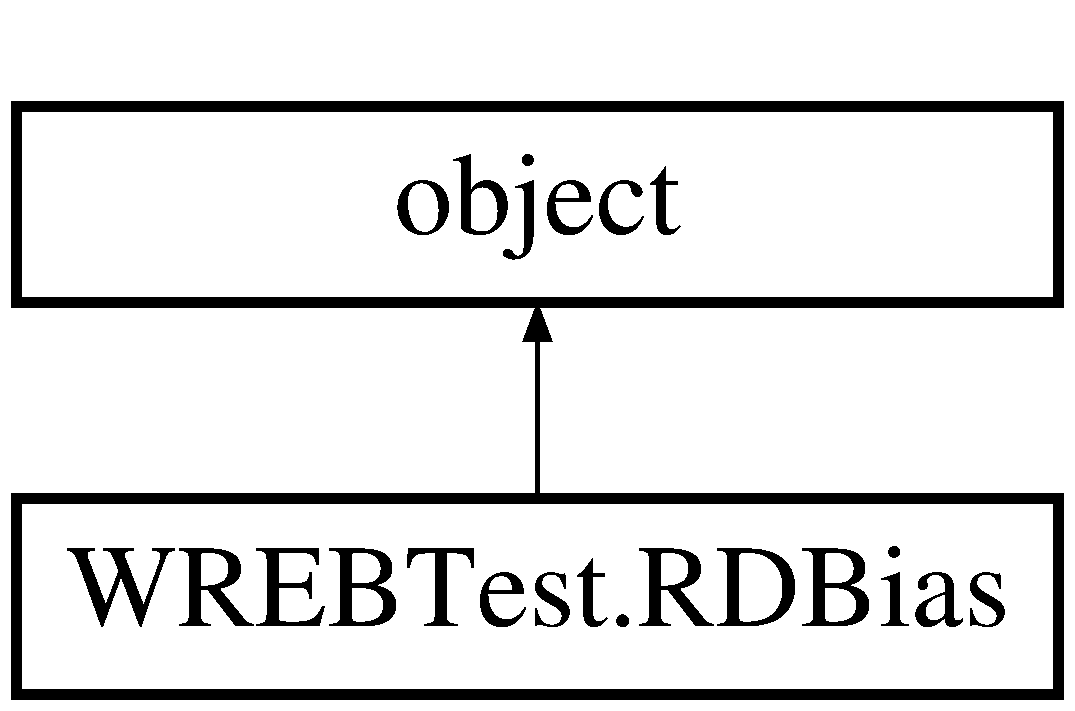
\includegraphics[height=2.000000cm]{class_w_r_e_b_test_1_1_r_d_bias}
\end{center}
\end{figure}
\subsection*{Public Member Functions}
\begin{DoxyCompactItemize}
\item 
def \hyperlink{class_w_r_e_b_test_1_1_r_d_bias_acc742bc1a44bbba81ab903a532aa2340}{\+\_\+\+\_\+init\+\_\+\+\_\+} (self)
\begin{DoxyCompactList}\small\item\em Initialize minimum required variables for test list. \end{DoxyCompactList}\item 
def \hyperlink{class_w_r_e_b_test_1_1_r_d_bias_aa0e5d7ab0c7193c74cd2f1940e31e46f}{run\+Test} (self)
\begin{DoxyCompactList}\small\item\em Run the test, save output to state variables. \end{DoxyCompactList}\item 
def \hyperlink{class_w_r_e_b_test_1_1_r_d_bias_ae17b85a71baa044098cd474ca12c4155}{summarize} (self, summary)
\begin{DoxyCompactList}\small\item\em Summarize the test results for the cover page of the report. \end{DoxyCompactList}\item 
def \hyperlink{class_w_r_e_b_test_1_1_r_d_bias_a411e7e21cb4b0603d8f2ed04b332ace4}{report} (self, pdf)
\begin{DoxyCompactList}\small\item\em generate this test\textquotesingle{}s page in the P\+DF report. \end{DoxyCompactList}\end{DoxyCompactItemize}


\subsection{Detailed Description}
Tests the reset drain performance. 



\subsection{Constructor \& Destructor Documentation}
\index{W\+R\+E\+B\+Test\+::\+R\+D\+Bias@{W\+R\+E\+B\+Test\+::\+R\+D\+Bias}!\+\_\+\+\_\+init\+\_\+\+\_\+@{\+\_\+\+\_\+init\+\_\+\+\_\+}}
\index{\+\_\+\+\_\+init\+\_\+\+\_\+@{\+\_\+\+\_\+init\+\_\+\+\_\+}!W\+R\+E\+B\+Test\+::\+R\+D\+Bias@{W\+R\+E\+B\+Test\+::\+R\+D\+Bias}}
\subsubsection[{\texorpdfstring{\+\_\+\+\_\+init\+\_\+\+\_\+(self)}{__init__(self)}}]{\setlength{\rightskip}{0pt plus 5cm}def W\+R\+E\+B\+Test.\+R\+D\+Bias.\+\_\+\+\_\+init\+\_\+\+\_\+ (
\begin{DoxyParamCaption}
\item[{}]{self}
\end{DoxyParamCaption}
)}\hypertarget{class_w_r_e_b_test_1_1_r_d_bias_acc742bc1a44bbba81ab903a532aa2340}{}\label{class_w_r_e_b_test_1_1_r_d_bias_acc742bc1a44bbba81ab903a532aa2340}


Initialize minimum required variables for test list. 



\subsection{Member Function Documentation}
\index{W\+R\+E\+B\+Test\+::\+R\+D\+Bias@{W\+R\+E\+B\+Test\+::\+R\+D\+Bias}!report@{report}}
\index{report@{report}!W\+R\+E\+B\+Test\+::\+R\+D\+Bias@{W\+R\+E\+B\+Test\+::\+R\+D\+Bias}}
\subsubsection[{\texorpdfstring{report(self, pdf)}{report(self, pdf)}}]{\setlength{\rightskip}{0pt plus 5cm}def W\+R\+E\+B\+Test.\+R\+D\+Bias.\+report (
\begin{DoxyParamCaption}
\item[{}]{self, }
\item[{}]{pdf}
\end{DoxyParamCaption}
)}\hypertarget{class_w_r_e_b_test_1_1_r_d_bias_a411e7e21cb4b0603d8f2ed04b332ace4}{}\label{class_w_r_e_b_test_1_1_r_d_bias_a411e7e21cb4b0603d8f2ed04b332ace4}


generate this test\textquotesingle{}s page in the P\+DF report. 


\begin{DoxyParams}{Parameters}
{\em pdf} & pyfpdf-\/compatible P\+DF object. \\
\hline
\end{DoxyParams}
\index{W\+R\+E\+B\+Test\+::\+R\+D\+Bias@{W\+R\+E\+B\+Test\+::\+R\+D\+Bias}!run\+Test@{run\+Test}}
\index{run\+Test@{run\+Test}!W\+R\+E\+B\+Test\+::\+R\+D\+Bias@{W\+R\+E\+B\+Test\+::\+R\+D\+Bias}}
\subsubsection[{\texorpdfstring{run\+Test(self)}{runTest(self)}}]{\setlength{\rightskip}{0pt plus 5cm}def W\+R\+E\+B\+Test.\+R\+D\+Bias.\+run\+Test (
\begin{DoxyParamCaption}
\item[{}]{self}
\end{DoxyParamCaption}
)}\hypertarget{class_w_r_e_b_test_1_1_r_d_bias_aa0e5d7ab0c7193c74cd2f1940e31e46f}{}\label{class_w_r_e_b_test_1_1_r_d_bias_aa0e5d7ab0c7193c74cd2f1940e31e46f}


Run the test, save output to state variables. 

\index{W\+R\+E\+B\+Test\+::\+R\+D\+Bias@{W\+R\+E\+B\+Test\+::\+R\+D\+Bias}!summarize@{summarize}}
\index{summarize@{summarize}!W\+R\+E\+B\+Test\+::\+R\+D\+Bias@{W\+R\+E\+B\+Test\+::\+R\+D\+Bias}}
\subsubsection[{\texorpdfstring{summarize(self, summary)}{summarize(self, summary)}}]{\setlength{\rightskip}{0pt plus 5cm}def W\+R\+E\+B\+Test.\+R\+D\+Bias.\+summarize (
\begin{DoxyParamCaption}
\item[{}]{self, }
\item[{}]{summary}
\end{DoxyParamCaption}
)}\hypertarget{class_w_r_e_b_test_1_1_r_d_bias_ae17b85a71baa044098cd474ca12c4155}{}\label{class_w_r_e_b_test_1_1_r_d_bias_ae17b85a71baa044098cd474ca12c4155}


Summarize the test results for the cover page of the report. 


\begin{DoxyParams}{Parameters}
{\em summary} & \hyperlink{class_w_r_e_b_test_1_1_summary}{Summary} obejct passed from Functional\+Test() \\
\hline
\end{DoxyParams}


The documentation for this class was generated from the following file\+:\begin{DoxyCompactItemize}
\item 
\hyperlink{_w_r_e_b_test_8py}{W\+R\+E\+B\+Test.\+py}\end{DoxyCompactItemize}

\hypertarget{class_v_s_t_test_1_1_r_g_rails}{}\section{V\+S\+T\+Test.\+R\+G\+Rails Class Reference}
\label{class_v_s_t_test_1_1_r_g_rails}\index{V\+S\+T\+Test.\+R\+G\+Rails@{V\+S\+T\+Test.\+R\+G\+Rails}}


Tests the reset gate rail performance.  


Inheritance diagram for V\+S\+T\+Test.\+R\+G\+Rails\+:\begin{figure}[H]
\begin{center}
\leavevmode
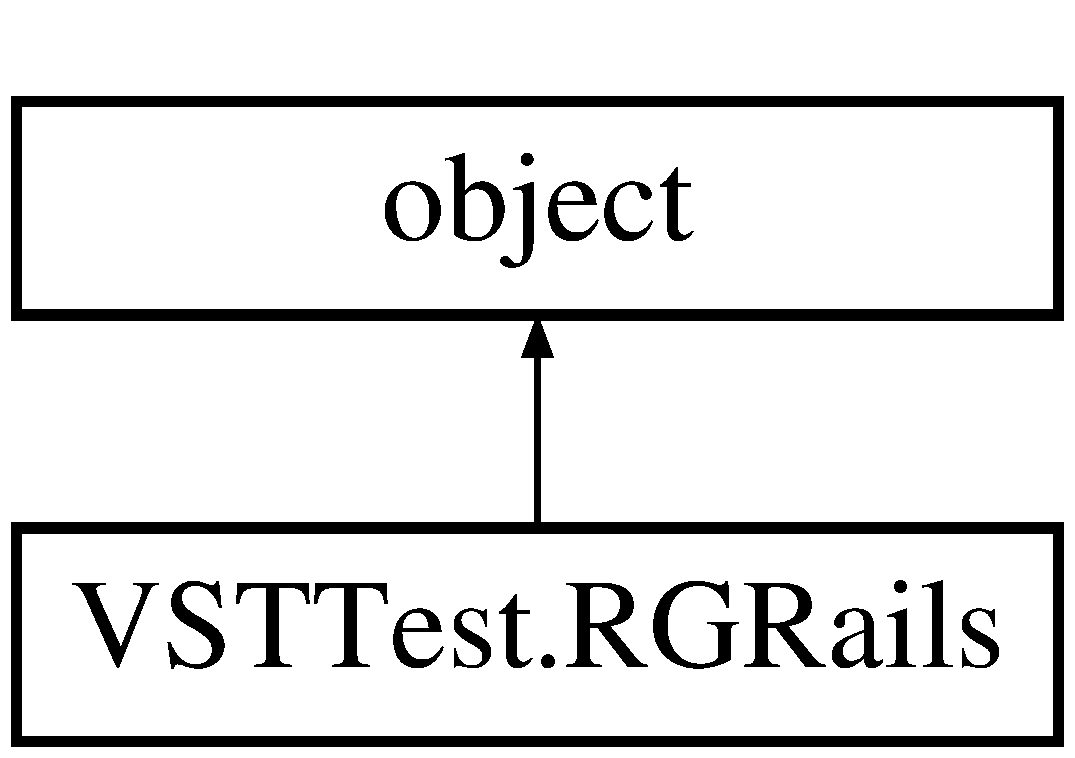
\includegraphics[height=2.000000cm]{class_v_s_t_test_1_1_r_g_rails}
\end{center}
\end{figure}
\subsection*{Public Member Functions}
\begin{DoxyCompactItemize}
\item 
def \hyperlink{class_v_s_t_test_1_1_r_g_rails_a85c267c8fae70d3556cb644b2d842443}{\+\_\+\+\_\+init\+\_\+\+\_\+} (self)
\begin{DoxyCompactList}\small\item\em Initialize minimum required variables for test list. \end{DoxyCompactList}\item 
def \hyperlink{class_v_s_t_test_1_1_r_g_rails_a1772c077dfe85be836e164434dcabcc1}{run\+Test} (self)
\begin{DoxyCompactList}\small\item\em Run the test, save output to state variables. \end{DoxyCompactList}\item 
def \hyperlink{class_v_s_t_test_1_1_r_g_rails_ae94665bd258b7b590bd41ccca4d4cb66}{summarize} (self, summary)
\begin{DoxyCompactList}\small\item\em Summarize the test results for the cover page of the report. \end{DoxyCompactList}\item 
def \hyperlink{class_v_s_t_test_1_1_r_g_rails_ad57a9f83959b1f24242f2179632b5c9f}{report} (self, pdf, report\+Path)
\begin{DoxyCompactList}\small\item\em generate this test\textquotesingle{}s page in the P\+DF report. \end{DoxyCompactList}\end{DoxyCompactItemize}


\subsection{Detailed Description}
Tests the reset gate rail performance. 



\subsection{Constructor \& Destructor Documentation}
\index{V\+S\+T\+Test\+::\+R\+G\+Rails@{V\+S\+T\+Test\+::\+R\+G\+Rails}!\+\_\+\+\_\+init\+\_\+\+\_\+@{\+\_\+\+\_\+init\+\_\+\+\_\+}}
\index{\+\_\+\+\_\+init\+\_\+\+\_\+@{\+\_\+\+\_\+init\+\_\+\+\_\+}!V\+S\+T\+Test\+::\+R\+G\+Rails@{V\+S\+T\+Test\+::\+R\+G\+Rails}}
\subsubsection[{\texorpdfstring{\+\_\+\+\_\+init\+\_\+\+\_\+(self)}{__init__(self)}}]{\setlength{\rightskip}{0pt plus 5cm}def V\+S\+T\+Test.\+R\+G\+Rails.\+\_\+\+\_\+init\+\_\+\+\_\+ (
\begin{DoxyParamCaption}
\item[{}]{self}
\end{DoxyParamCaption}
)}\hypertarget{class_v_s_t_test_1_1_r_g_rails_a85c267c8fae70d3556cb644b2d842443}{}\label{class_v_s_t_test_1_1_r_g_rails_a85c267c8fae70d3556cb644b2d842443}


Initialize minimum required variables for test list. 



\subsection{Member Function Documentation}
\index{V\+S\+T\+Test\+::\+R\+G\+Rails@{V\+S\+T\+Test\+::\+R\+G\+Rails}!report@{report}}
\index{report@{report}!V\+S\+T\+Test\+::\+R\+G\+Rails@{V\+S\+T\+Test\+::\+R\+G\+Rails}}
\subsubsection[{\texorpdfstring{report(self, pdf, report\+Path)}{report(self, pdf, reportPath)}}]{\setlength{\rightskip}{0pt plus 5cm}def V\+S\+T\+Test.\+R\+G\+Rails.\+report (
\begin{DoxyParamCaption}
\item[{}]{self, }
\item[{}]{pdf, }
\item[{}]{report\+Path}
\end{DoxyParamCaption}
)}\hypertarget{class_v_s_t_test_1_1_r_g_rails_ad57a9f83959b1f24242f2179632b5c9f}{}\label{class_v_s_t_test_1_1_r_g_rails_ad57a9f83959b1f24242f2179632b5c9f}


generate this test\textquotesingle{}s page in the P\+DF report. 


\begin{DoxyParams}{Parameters}
{\em pdf} & pyfpdf-\/compatible P\+DF object. \\
\hline
{\em report\+Path} & Path of directory containing the pdf report \\
\hline
\end{DoxyParams}
\index{V\+S\+T\+Test\+::\+R\+G\+Rails@{V\+S\+T\+Test\+::\+R\+G\+Rails}!run\+Test@{run\+Test}}
\index{run\+Test@{run\+Test}!V\+S\+T\+Test\+::\+R\+G\+Rails@{V\+S\+T\+Test\+::\+R\+G\+Rails}}
\subsubsection[{\texorpdfstring{run\+Test(self)}{runTest(self)}}]{\setlength{\rightskip}{0pt plus 5cm}def V\+S\+T\+Test.\+R\+G\+Rails.\+run\+Test (
\begin{DoxyParamCaption}
\item[{}]{self}
\end{DoxyParamCaption}
)}\hypertarget{class_v_s_t_test_1_1_r_g_rails_a1772c077dfe85be836e164434dcabcc1}{}\label{class_v_s_t_test_1_1_r_g_rails_a1772c077dfe85be836e164434dcabcc1}


Run the test, save output to state variables. 

\index{V\+S\+T\+Test\+::\+R\+G\+Rails@{V\+S\+T\+Test\+::\+R\+G\+Rails}!summarize@{summarize}}
\index{summarize@{summarize}!V\+S\+T\+Test\+::\+R\+G\+Rails@{V\+S\+T\+Test\+::\+R\+G\+Rails}}
\subsubsection[{\texorpdfstring{summarize(self, summary)}{summarize(self, summary)}}]{\setlength{\rightskip}{0pt plus 5cm}def V\+S\+T\+Test.\+R\+G\+Rails.\+summarize (
\begin{DoxyParamCaption}
\item[{}]{self, }
\item[{}]{summary}
\end{DoxyParamCaption}
)}\hypertarget{class_v_s_t_test_1_1_r_g_rails_ae94665bd258b7b590bd41ccca4d4cb66}{}\label{class_v_s_t_test_1_1_r_g_rails_ae94665bd258b7b590bd41ccca4d4cb66}


Summarize the test results for the cover page of the report. 


\begin{DoxyParams}{Parameters}
{\em summary} & \hyperlink{class_v_s_t_test_1_1_summary}{Summary} obejct passed from Functional\+Test() \\
\hline
\end{DoxyParams}


The documentation for this class was generated from the following file\+:\begin{DoxyCompactItemize}
\item 
\hyperlink{_v_s_t_test_8py}{V\+S\+T\+Test.\+py}\end{DoxyCompactItemize}

\hypertarget{class_g_r_e_b_test_1_1_r_g_rails}{}\section{G\+R\+E\+B\+Test.\+R\+G\+Rails Class Reference}
\label{class_g_r_e_b_test_1_1_r_g_rails}\index{G\+R\+E\+B\+Test.\+R\+G\+Rails@{G\+R\+E\+B\+Test.\+R\+G\+Rails}}


Tests the reset gate rail performance.  


Inheritance diagram for G\+R\+E\+B\+Test.\+R\+G\+Rails\+:\begin{figure}[H]
\begin{center}
\leavevmode
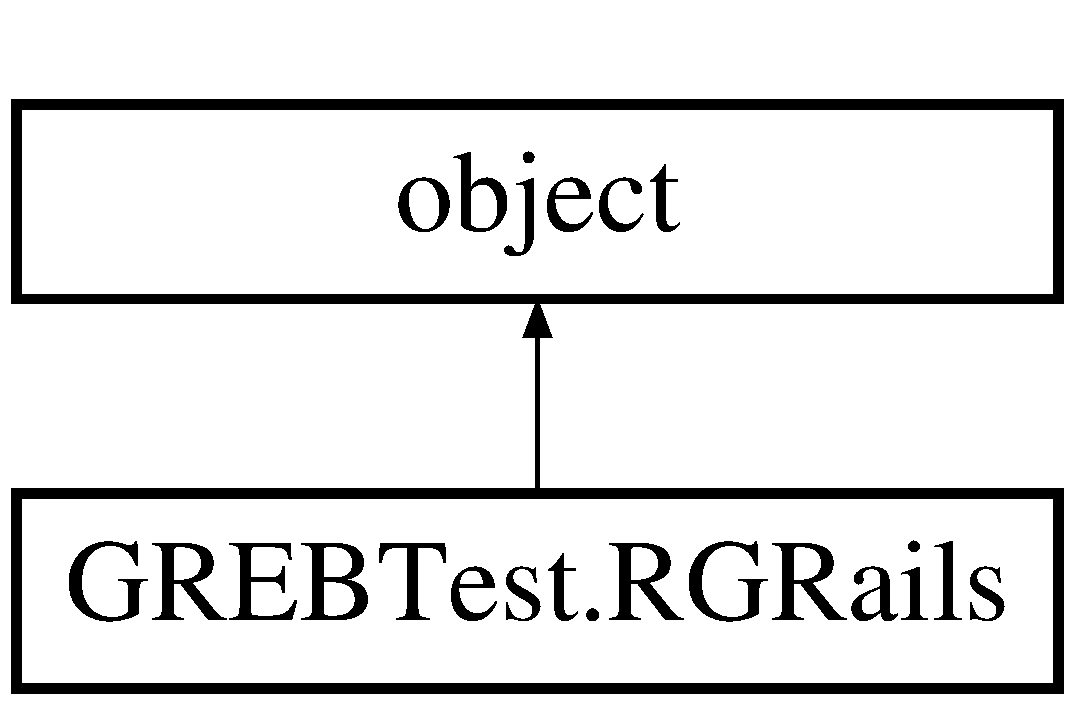
\includegraphics[height=2.000000cm]{class_g_r_e_b_test_1_1_r_g_rails}
\end{center}
\end{figure}
\subsection*{Public Member Functions}
\begin{DoxyCompactItemize}
\item 
def \hyperlink{class_g_r_e_b_test_1_1_r_g_rails_ad5c0e5b8b5c15405baa9a904cb88ba29}{\+\_\+\+\_\+init\+\_\+\+\_\+} (self)
\begin{DoxyCompactList}\small\item\em Initialize minimum required variables for test list. \end{DoxyCompactList}\item 
def \hyperlink{class_g_r_e_b_test_1_1_r_g_rails_a0626f52ae5a531fbd25a5e3e0e4fb532}{run\+Test} (self)
\begin{DoxyCompactList}\small\item\em Run the test, save output to state variables. \end{DoxyCompactList}\item 
def \hyperlink{class_g_r_e_b_test_1_1_r_g_rails_aab4387f319014e2b2cdc5ca58b15e780}{summarize} (self, summary)
\begin{DoxyCompactList}\small\item\em Summarize the test results for the cover page of the report. \end{DoxyCompactList}\item 
def \hyperlink{class_g_r_e_b_test_1_1_r_g_rails_a49d56a3d9cf180e8d128136e9ddb23e2}{report} (self, pdf, report\+Path)
\begin{DoxyCompactList}\small\item\em generate this test\textquotesingle{}s page in the P\+DF report. \end{DoxyCompactList}\end{DoxyCompactItemize}


\subsection{Detailed Description}
Tests the reset gate rail performance. 



\subsection{Constructor \& Destructor Documentation}
\index{G\+R\+E\+B\+Test\+::\+R\+G\+Rails@{G\+R\+E\+B\+Test\+::\+R\+G\+Rails}!\+\_\+\+\_\+init\+\_\+\+\_\+@{\+\_\+\+\_\+init\+\_\+\+\_\+}}
\index{\+\_\+\+\_\+init\+\_\+\+\_\+@{\+\_\+\+\_\+init\+\_\+\+\_\+}!G\+R\+E\+B\+Test\+::\+R\+G\+Rails@{G\+R\+E\+B\+Test\+::\+R\+G\+Rails}}
\subsubsection[{\texorpdfstring{\+\_\+\+\_\+init\+\_\+\+\_\+(self)}{__init__(self)}}]{\setlength{\rightskip}{0pt plus 5cm}def G\+R\+E\+B\+Test.\+R\+G\+Rails.\+\_\+\+\_\+init\+\_\+\+\_\+ (
\begin{DoxyParamCaption}
\item[{}]{self}
\end{DoxyParamCaption}
)}\hypertarget{class_g_r_e_b_test_1_1_r_g_rails_ad5c0e5b8b5c15405baa9a904cb88ba29}{}\label{class_g_r_e_b_test_1_1_r_g_rails_ad5c0e5b8b5c15405baa9a904cb88ba29}


Initialize minimum required variables for test list. 



\subsection{Member Function Documentation}
\index{G\+R\+E\+B\+Test\+::\+R\+G\+Rails@{G\+R\+E\+B\+Test\+::\+R\+G\+Rails}!report@{report}}
\index{report@{report}!G\+R\+E\+B\+Test\+::\+R\+G\+Rails@{G\+R\+E\+B\+Test\+::\+R\+G\+Rails}}
\subsubsection[{\texorpdfstring{report(self, pdf, report\+Path)}{report(self, pdf, reportPath)}}]{\setlength{\rightskip}{0pt plus 5cm}def G\+R\+E\+B\+Test.\+R\+G\+Rails.\+report (
\begin{DoxyParamCaption}
\item[{}]{self, }
\item[{}]{pdf, }
\item[{}]{report\+Path}
\end{DoxyParamCaption}
)}\hypertarget{class_g_r_e_b_test_1_1_r_g_rails_a49d56a3d9cf180e8d128136e9ddb23e2}{}\label{class_g_r_e_b_test_1_1_r_g_rails_a49d56a3d9cf180e8d128136e9ddb23e2}


generate this test\textquotesingle{}s page in the P\+DF report. 


\begin{DoxyParams}{Parameters}
{\em pdf} & pyfpdf-\/compatible P\+DF object. \\
\hline
{\em report\+Path} & Path of directory containing the pdf report \\
\hline
\end{DoxyParams}
\index{G\+R\+E\+B\+Test\+::\+R\+G\+Rails@{G\+R\+E\+B\+Test\+::\+R\+G\+Rails}!run\+Test@{run\+Test}}
\index{run\+Test@{run\+Test}!G\+R\+E\+B\+Test\+::\+R\+G\+Rails@{G\+R\+E\+B\+Test\+::\+R\+G\+Rails}}
\subsubsection[{\texorpdfstring{run\+Test(self)}{runTest(self)}}]{\setlength{\rightskip}{0pt plus 5cm}def G\+R\+E\+B\+Test.\+R\+G\+Rails.\+run\+Test (
\begin{DoxyParamCaption}
\item[{}]{self}
\end{DoxyParamCaption}
)}\hypertarget{class_g_r_e_b_test_1_1_r_g_rails_a0626f52ae5a531fbd25a5e3e0e4fb532}{}\label{class_g_r_e_b_test_1_1_r_g_rails_a0626f52ae5a531fbd25a5e3e0e4fb532}


Run the test, save output to state variables. 

\index{G\+R\+E\+B\+Test\+::\+R\+G\+Rails@{G\+R\+E\+B\+Test\+::\+R\+G\+Rails}!summarize@{summarize}}
\index{summarize@{summarize}!G\+R\+E\+B\+Test\+::\+R\+G\+Rails@{G\+R\+E\+B\+Test\+::\+R\+G\+Rails}}
\subsubsection[{\texorpdfstring{summarize(self, summary)}{summarize(self, summary)}}]{\setlength{\rightskip}{0pt plus 5cm}def G\+R\+E\+B\+Test.\+R\+G\+Rails.\+summarize (
\begin{DoxyParamCaption}
\item[{}]{self, }
\item[{}]{summary}
\end{DoxyParamCaption}
)}\hypertarget{class_g_r_e_b_test_1_1_r_g_rails_aab4387f319014e2b2cdc5ca58b15e780}{}\label{class_g_r_e_b_test_1_1_r_g_rails_aab4387f319014e2b2cdc5ca58b15e780}


Summarize the test results for the cover page of the report. 


\begin{DoxyParams}{Parameters}
{\em summary} & \hyperlink{class_g_r_e_b_test_1_1_summary}{Summary} obejct passed from Functional\+Test() \\
\hline
\end{DoxyParams}


The documentation for this class was generated from the following file\+:\begin{DoxyCompactItemize}
\item 
\hyperlink{_g_r_e_b_test_8py}{G\+R\+E\+B\+Test.\+py}\end{DoxyCompactItemize}

\hypertarget{class_w_r_e_b_test_1_1_r_g_rails}{}\section{W\+R\+E\+B\+Test.\+R\+G\+Rails Class Reference}
\label{class_w_r_e_b_test_1_1_r_g_rails}\index{W\+R\+E\+B\+Test.\+R\+G\+Rails@{W\+R\+E\+B\+Test.\+R\+G\+Rails}}


Tests the reset gate rail performance.  


Inheritance diagram for W\+R\+E\+B\+Test.\+R\+G\+Rails\+:\begin{figure}[H]
\begin{center}
\leavevmode
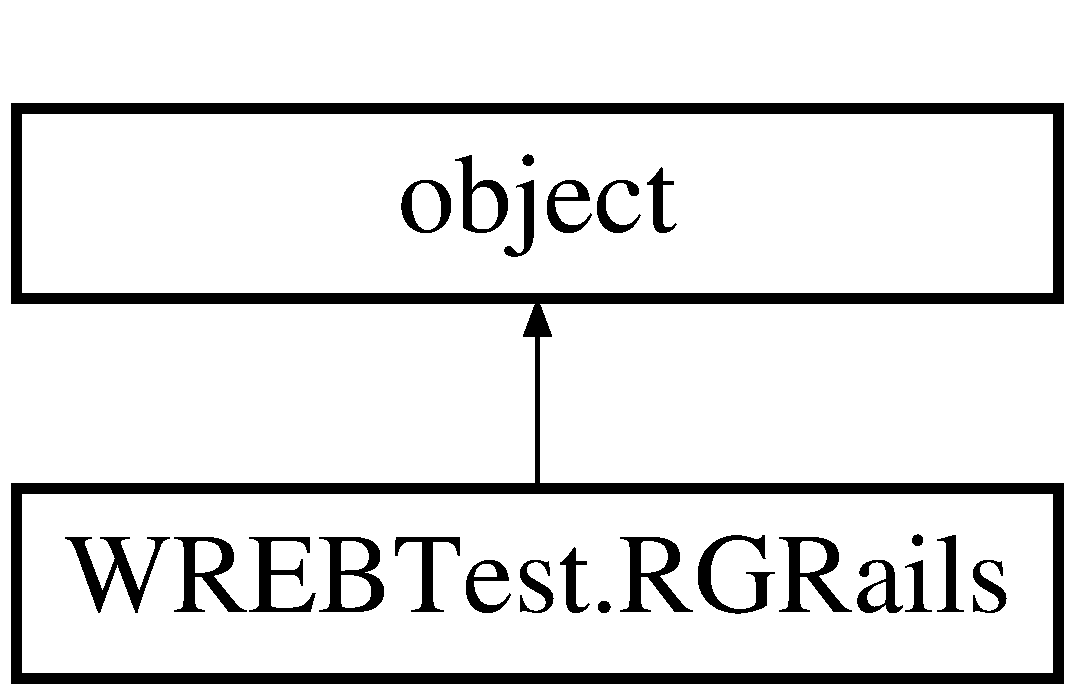
\includegraphics[height=2.000000cm]{class_w_r_e_b_test_1_1_r_g_rails}
\end{center}
\end{figure}
\subsection*{Public Member Functions}
\begin{DoxyCompactItemize}
\item 
def \hyperlink{class_w_r_e_b_test_1_1_r_g_rails_aa88fe8bf073459ccdd221172f50bf78c}{\+\_\+\+\_\+init\+\_\+\+\_\+} (self)
\begin{DoxyCompactList}\small\item\em Initialize minimum required variables for test list. \end{DoxyCompactList}\item 
def \hyperlink{class_w_r_e_b_test_1_1_r_g_rails_ad734ff3e10aac9d80365f55dc88f5adc}{run\+Test} (self)
\begin{DoxyCompactList}\small\item\em Run the test, save output to state variables. \end{DoxyCompactList}\item 
def \hyperlink{class_w_r_e_b_test_1_1_r_g_rails_a7c0b9c673b50fdaa24e1911a0634adca}{summarize} (self, summary)
\begin{DoxyCompactList}\small\item\em Summarize the test results for the cover page of the report. \end{DoxyCompactList}\item 
def \hyperlink{class_w_r_e_b_test_1_1_r_g_rails_a7736f682d02c1200e55ec3e587556c54}{report} (self, pdf, report\+Path)
\begin{DoxyCompactList}\small\item\em generate this test\textquotesingle{}s page in the P\+DF report. \end{DoxyCompactList}\end{DoxyCompactItemize}


\subsection{Detailed Description}
Tests the reset gate rail performance. 



\subsection{Constructor \& Destructor Documentation}
\index{W\+R\+E\+B\+Test\+::\+R\+G\+Rails@{W\+R\+E\+B\+Test\+::\+R\+G\+Rails}!\+\_\+\+\_\+init\+\_\+\+\_\+@{\+\_\+\+\_\+init\+\_\+\+\_\+}}
\index{\+\_\+\+\_\+init\+\_\+\+\_\+@{\+\_\+\+\_\+init\+\_\+\+\_\+}!W\+R\+E\+B\+Test\+::\+R\+G\+Rails@{W\+R\+E\+B\+Test\+::\+R\+G\+Rails}}
\subsubsection[{\texorpdfstring{\+\_\+\+\_\+init\+\_\+\+\_\+(self)}{__init__(self)}}]{\setlength{\rightskip}{0pt plus 5cm}def W\+R\+E\+B\+Test.\+R\+G\+Rails.\+\_\+\+\_\+init\+\_\+\+\_\+ (
\begin{DoxyParamCaption}
\item[{}]{self}
\end{DoxyParamCaption}
)}\hypertarget{class_w_r_e_b_test_1_1_r_g_rails_aa88fe8bf073459ccdd221172f50bf78c}{}\label{class_w_r_e_b_test_1_1_r_g_rails_aa88fe8bf073459ccdd221172f50bf78c}


Initialize minimum required variables for test list. 



\subsection{Member Function Documentation}
\index{W\+R\+E\+B\+Test\+::\+R\+G\+Rails@{W\+R\+E\+B\+Test\+::\+R\+G\+Rails}!report@{report}}
\index{report@{report}!W\+R\+E\+B\+Test\+::\+R\+G\+Rails@{W\+R\+E\+B\+Test\+::\+R\+G\+Rails}}
\subsubsection[{\texorpdfstring{report(self, pdf, report\+Path)}{report(self, pdf, reportPath)}}]{\setlength{\rightskip}{0pt plus 5cm}def W\+R\+E\+B\+Test.\+R\+G\+Rails.\+report (
\begin{DoxyParamCaption}
\item[{}]{self, }
\item[{}]{pdf, }
\item[{}]{report\+Path}
\end{DoxyParamCaption}
)}\hypertarget{class_w_r_e_b_test_1_1_r_g_rails_a7736f682d02c1200e55ec3e587556c54}{}\label{class_w_r_e_b_test_1_1_r_g_rails_a7736f682d02c1200e55ec3e587556c54}


generate this test\textquotesingle{}s page in the P\+DF report. 


\begin{DoxyParams}{Parameters}
{\em pdf} & pyfpdf-\/compatible P\+DF object. \\
\hline
{\em report\+Path} & Path of directory containing the pdf report \\
\hline
\end{DoxyParams}
\index{W\+R\+E\+B\+Test\+::\+R\+G\+Rails@{W\+R\+E\+B\+Test\+::\+R\+G\+Rails}!run\+Test@{run\+Test}}
\index{run\+Test@{run\+Test}!W\+R\+E\+B\+Test\+::\+R\+G\+Rails@{W\+R\+E\+B\+Test\+::\+R\+G\+Rails}}
\subsubsection[{\texorpdfstring{run\+Test(self)}{runTest(self)}}]{\setlength{\rightskip}{0pt plus 5cm}def W\+R\+E\+B\+Test.\+R\+G\+Rails.\+run\+Test (
\begin{DoxyParamCaption}
\item[{}]{self}
\end{DoxyParamCaption}
)}\hypertarget{class_w_r_e_b_test_1_1_r_g_rails_ad734ff3e10aac9d80365f55dc88f5adc}{}\label{class_w_r_e_b_test_1_1_r_g_rails_ad734ff3e10aac9d80365f55dc88f5adc}


Run the test, save output to state variables. 

\index{W\+R\+E\+B\+Test\+::\+R\+G\+Rails@{W\+R\+E\+B\+Test\+::\+R\+G\+Rails}!summarize@{summarize}}
\index{summarize@{summarize}!W\+R\+E\+B\+Test\+::\+R\+G\+Rails@{W\+R\+E\+B\+Test\+::\+R\+G\+Rails}}
\subsubsection[{\texorpdfstring{summarize(self, summary)}{summarize(self, summary)}}]{\setlength{\rightskip}{0pt plus 5cm}def W\+R\+E\+B\+Test.\+R\+G\+Rails.\+summarize (
\begin{DoxyParamCaption}
\item[{}]{self, }
\item[{}]{summary}
\end{DoxyParamCaption}
)}\hypertarget{class_w_r_e_b_test_1_1_r_g_rails_a7c0b9c673b50fdaa24e1911a0634adca}{}\label{class_w_r_e_b_test_1_1_r_g_rails_a7c0b9c673b50fdaa24e1911a0634adca}


Summarize the test results for the cover page of the report. 


\begin{DoxyParams}{Parameters}
{\em summary} & \hyperlink{class_w_r_e_b_test_1_1_summary}{Summary} obejct passed from Functional\+Test() \\
\hline
\end{DoxyParams}


The documentation for this class was generated from the following file\+:\begin{DoxyCompactItemize}
\item 
\hyperlink{_w_r_e_b_test_8py}{W\+R\+E\+B\+Test.\+py}\end{DoxyCompactItemize}

\hypertarget{class_v_s_t_test_1_1_r_g_rails_diverging}{}\section{V\+S\+T\+Test.\+R\+G\+Rails\+Diverging Class Reference}
\label{class_v_s_t_test_1_1_r_g_rails_diverging}\index{V\+S\+T\+Test.\+R\+G\+Rails\+Diverging@{V\+S\+T\+Test.\+R\+G\+Rails\+Diverging}}


Tests the reset gate rail performance with a diverging voltage pattern.  


Inheritance diagram for V\+S\+T\+Test.\+R\+G\+Rails\+Diverging\+:\begin{figure}[H]
\begin{center}
\leavevmode
\includegraphics[height=2.000000cm]{class_v_s_t_test_1_1_r_g_rails_diverging}
\end{center}
\end{figure}
\subsection*{Public Member Functions}
\begin{DoxyCompactItemize}
\item 
def \hyperlink{class_v_s_t_test_1_1_r_g_rails_diverging_a3e9f3ea44f1cebae255b767668a63033}{\+\_\+\+\_\+init\+\_\+\+\_\+} (self, amplitude, startV)
\begin{DoxyCompactList}\small\item\em Initialize required variables for test list and stores input arguments to state variables. \end{DoxyCompactList}\item 
def \hyperlink{class_v_s_t_test_1_1_r_g_rails_diverging_a9a27de681058f113edc6acabf0034e28}{run\+Test} (self)
\begin{DoxyCompactList}\small\item\em Run the test, save output to state variables. \end{DoxyCompactList}\item 
def \hyperlink{class_v_s_t_test_1_1_r_g_rails_diverging_a5a6964f3dfda21365e3c581e85b5a31e}{summarize} (self, summary)
\begin{DoxyCompactList}\small\item\em Summarize the test results for the cover page of the report. \end{DoxyCompactList}\item 
def \hyperlink{class_v_s_t_test_1_1_r_g_rails_diverging_ab88a31c9d04ed4f1cdb17bd17544df40}{report} (self, pdf, report\+Path)
\begin{DoxyCompactList}\small\item\em generate this test\textquotesingle{}s page in the P\+DF report. \end{DoxyCompactList}\end{DoxyCompactItemize}


\subsection{Detailed Description}
Tests the reset gate rail performance with a diverging voltage pattern. 



\subsection{Constructor \& Destructor Documentation}
\index{V\+S\+T\+Test\+::\+R\+G\+Rails\+Diverging@{V\+S\+T\+Test\+::\+R\+G\+Rails\+Diverging}!\+\_\+\+\_\+init\+\_\+\+\_\+@{\+\_\+\+\_\+init\+\_\+\+\_\+}}
\index{\+\_\+\+\_\+init\+\_\+\+\_\+@{\+\_\+\+\_\+init\+\_\+\+\_\+}!V\+S\+T\+Test\+::\+R\+G\+Rails\+Diverging@{V\+S\+T\+Test\+::\+R\+G\+Rails\+Diverging}}
\subsubsection[{\texorpdfstring{\+\_\+\+\_\+init\+\_\+\+\_\+(self, amplitude, start\+V)}{__init__(self, amplitude, startV)}}]{\setlength{\rightskip}{0pt plus 5cm}def V\+S\+T\+Test.\+R\+G\+Rails\+Diverging.\+\_\+\+\_\+init\+\_\+\+\_\+ (
\begin{DoxyParamCaption}
\item[{}]{self, }
\item[{}]{amplitude, }
\item[{}]{startV}
\end{DoxyParamCaption}
)}\hypertarget{class_v_s_t_test_1_1_r_g_rails_diverging_a3e9f3ea44f1cebae255b767668a63033}{}\label{class_v_s_t_test_1_1_r_g_rails_diverging_a3e9f3ea44f1cebae255b767668a63033}


Initialize required variables for test list and stores input arguments to state variables. 


\begin{DoxyParams}{Parameters}
{\em amplitude} & Maximum voltage differential between rails, half-\/wave. (5V amplitude is 10V max difference.) \\
\hline
{\em startV} & Initial voltage the diverging rails tests starts at. \\
\hline
\end{DoxyParams}


\subsection{Member Function Documentation}
\index{V\+S\+T\+Test\+::\+R\+G\+Rails\+Diverging@{V\+S\+T\+Test\+::\+R\+G\+Rails\+Diverging}!report@{report}}
\index{report@{report}!V\+S\+T\+Test\+::\+R\+G\+Rails\+Diverging@{V\+S\+T\+Test\+::\+R\+G\+Rails\+Diverging}}
\subsubsection[{\texorpdfstring{report(self, pdf, report\+Path)}{report(self, pdf, reportPath)}}]{\setlength{\rightskip}{0pt plus 5cm}def V\+S\+T\+Test.\+R\+G\+Rails\+Diverging.\+report (
\begin{DoxyParamCaption}
\item[{}]{self, }
\item[{}]{pdf, }
\item[{}]{report\+Path}
\end{DoxyParamCaption}
)}\hypertarget{class_v_s_t_test_1_1_r_g_rails_diverging_ab88a31c9d04ed4f1cdb17bd17544df40}{}\label{class_v_s_t_test_1_1_r_g_rails_diverging_ab88a31c9d04ed4f1cdb17bd17544df40}


generate this test\textquotesingle{}s page in the P\+DF report. 


\begin{DoxyParams}{Parameters}
{\em pdf} & pyfpdf-\/compatible P\+DF object. \\
\hline
{\em report\+Path} & Path of directory containing the pdf report \\
\hline
\end{DoxyParams}
\index{V\+S\+T\+Test\+::\+R\+G\+Rails\+Diverging@{V\+S\+T\+Test\+::\+R\+G\+Rails\+Diverging}!run\+Test@{run\+Test}}
\index{run\+Test@{run\+Test}!V\+S\+T\+Test\+::\+R\+G\+Rails\+Diverging@{V\+S\+T\+Test\+::\+R\+G\+Rails\+Diverging}}
\subsubsection[{\texorpdfstring{run\+Test(self)}{runTest(self)}}]{\setlength{\rightskip}{0pt plus 5cm}def V\+S\+T\+Test.\+R\+G\+Rails\+Diverging.\+run\+Test (
\begin{DoxyParamCaption}
\item[{}]{self}
\end{DoxyParamCaption}
)}\hypertarget{class_v_s_t_test_1_1_r_g_rails_diverging_a9a27de681058f113edc6acabf0034e28}{}\label{class_v_s_t_test_1_1_r_g_rails_diverging_a9a27de681058f113edc6acabf0034e28}


Run the test, save output to state variables. 

\index{V\+S\+T\+Test\+::\+R\+G\+Rails\+Diverging@{V\+S\+T\+Test\+::\+R\+G\+Rails\+Diverging}!summarize@{summarize}}
\index{summarize@{summarize}!V\+S\+T\+Test\+::\+R\+G\+Rails\+Diverging@{V\+S\+T\+Test\+::\+R\+G\+Rails\+Diverging}}
\subsubsection[{\texorpdfstring{summarize(self, summary)}{summarize(self, summary)}}]{\setlength{\rightskip}{0pt plus 5cm}def V\+S\+T\+Test.\+R\+G\+Rails\+Diverging.\+summarize (
\begin{DoxyParamCaption}
\item[{}]{self, }
\item[{}]{summary}
\end{DoxyParamCaption}
)}\hypertarget{class_v_s_t_test_1_1_r_g_rails_diverging_a5a6964f3dfda21365e3c581e85b5a31e}{}\label{class_v_s_t_test_1_1_r_g_rails_diverging_a5a6964f3dfda21365e3c581e85b5a31e}


Summarize the test results for the cover page of the report. 


\begin{DoxyParams}{Parameters}
{\em summary} & \hyperlink{class_v_s_t_test_1_1_summary}{Summary} obejct passed from Functional\+Test() \\
\hline
\end{DoxyParams}


The documentation for this class was generated from the following file\+:\begin{DoxyCompactItemize}
\item 
\hyperlink{_v_s_t_test_8py}{V\+S\+T\+Test.\+py}\end{DoxyCompactItemize}

\hypertarget{class_g_r_e_b_test_1_1_r_g_rails_diverging}{}\section{G\+R\+E\+B\+Test.\+R\+G\+Rails\+Diverging Class Reference}
\label{class_g_r_e_b_test_1_1_r_g_rails_diverging}\index{G\+R\+E\+B\+Test.\+R\+G\+Rails\+Diverging@{G\+R\+E\+B\+Test.\+R\+G\+Rails\+Diverging}}


Tests the reset gate rail performance with a diverging voltage pattern.  


Inheritance diagram for G\+R\+E\+B\+Test.\+R\+G\+Rails\+Diverging\+:\begin{figure}[H]
\begin{center}
\leavevmode
\includegraphics[height=2.000000cm]{class_g_r_e_b_test_1_1_r_g_rails_diverging}
\end{center}
\end{figure}
\subsection*{Public Member Functions}
\begin{DoxyCompactItemize}
\item 
def \hyperlink{class_g_r_e_b_test_1_1_r_g_rails_diverging_a80bca507ab4c2c3d5e1821f7e81a34e8}{\+\_\+\+\_\+init\+\_\+\+\_\+} (self, amplitude, startV)
\begin{DoxyCompactList}\small\item\em Initialize required variables for test list and stores input arguments to state variables. \end{DoxyCompactList}\item 
def \hyperlink{class_g_r_e_b_test_1_1_r_g_rails_diverging_a34c944c556559bdf05bd5350833c1db6}{run\+Test} (self)
\begin{DoxyCompactList}\small\item\em Run the test, save output to state variables. \end{DoxyCompactList}\item 
def \hyperlink{class_g_r_e_b_test_1_1_r_g_rails_diverging_a262ac574eef44165ea30130e8145c683}{summarize} (self, summary)
\begin{DoxyCompactList}\small\item\em Summarize the test results for the cover page of the report. \end{DoxyCompactList}\item 
def \hyperlink{class_g_r_e_b_test_1_1_r_g_rails_diverging_a99618ce71adbb3a4d75b221941d629af}{report} (self, pdf, report\+Path)
\begin{DoxyCompactList}\small\item\em generate this test\textquotesingle{}s page in the P\+DF report. \end{DoxyCompactList}\end{DoxyCompactItemize}


\subsection{Detailed Description}
Tests the reset gate rail performance with a diverging voltage pattern. 



\subsection{Constructor \& Destructor Documentation}
\index{G\+R\+E\+B\+Test\+::\+R\+G\+Rails\+Diverging@{G\+R\+E\+B\+Test\+::\+R\+G\+Rails\+Diverging}!\+\_\+\+\_\+init\+\_\+\+\_\+@{\+\_\+\+\_\+init\+\_\+\+\_\+}}
\index{\+\_\+\+\_\+init\+\_\+\+\_\+@{\+\_\+\+\_\+init\+\_\+\+\_\+}!G\+R\+E\+B\+Test\+::\+R\+G\+Rails\+Diverging@{G\+R\+E\+B\+Test\+::\+R\+G\+Rails\+Diverging}}
\subsubsection[{\texorpdfstring{\+\_\+\+\_\+init\+\_\+\+\_\+(self, amplitude, start\+V)}{__init__(self, amplitude, startV)}}]{\setlength{\rightskip}{0pt plus 5cm}def G\+R\+E\+B\+Test.\+R\+G\+Rails\+Diverging.\+\_\+\+\_\+init\+\_\+\+\_\+ (
\begin{DoxyParamCaption}
\item[{}]{self, }
\item[{}]{amplitude, }
\item[{}]{startV}
\end{DoxyParamCaption}
)}\hypertarget{class_g_r_e_b_test_1_1_r_g_rails_diverging_a80bca507ab4c2c3d5e1821f7e81a34e8}{}\label{class_g_r_e_b_test_1_1_r_g_rails_diverging_a80bca507ab4c2c3d5e1821f7e81a34e8}


Initialize required variables for test list and stores input arguments to state variables. 


\begin{DoxyParams}{Parameters}
{\em amplitude} & Maximum voltage differential between rails, half-\/wave. (5V amplitude is 10V max difference.) \\
\hline
{\em startV} & Initial voltage the diverging rails tests starts at. \\
\hline
\end{DoxyParams}


\subsection{Member Function Documentation}
\index{G\+R\+E\+B\+Test\+::\+R\+G\+Rails\+Diverging@{G\+R\+E\+B\+Test\+::\+R\+G\+Rails\+Diverging}!report@{report}}
\index{report@{report}!G\+R\+E\+B\+Test\+::\+R\+G\+Rails\+Diverging@{G\+R\+E\+B\+Test\+::\+R\+G\+Rails\+Diverging}}
\subsubsection[{\texorpdfstring{report(self, pdf, report\+Path)}{report(self, pdf, reportPath)}}]{\setlength{\rightskip}{0pt plus 5cm}def G\+R\+E\+B\+Test.\+R\+G\+Rails\+Diverging.\+report (
\begin{DoxyParamCaption}
\item[{}]{self, }
\item[{}]{pdf, }
\item[{}]{report\+Path}
\end{DoxyParamCaption}
)}\hypertarget{class_g_r_e_b_test_1_1_r_g_rails_diverging_a99618ce71adbb3a4d75b221941d629af}{}\label{class_g_r_e_b_test_1_1_r_g_rails_diverging_a99618ce71adbb3a4d75b221941d629af}


generate this test\textquotesingle{}s page in the P\+DF report. 


\begin{DoxyParams}{Parameters}
{\em pdf} & pyfpdf-\/compatible P\+DF object. \\
\hline
{\em report\+Path} & Path of directory containing the pdf report \\
\hline
\end{DoxyParams}
\index{G\+R\+E\+B\+Test\+::\+R\+G\+Rails\+Diverging@{G\+R\+E\+B\+Test\+::\+R\+G\+Rails\+Diverging}!run\+Test@{run\+Test}}
\index{run\+Test@{run\+Test}!G\+R\+E\+B\+Test\+::\+R\+G\+Rails\+Diverging@{G\+R\+E\+B\+Test\+::\+R\+G\+Rails\+Diverging}}
\subsubsection[{\texorpdfstring{run\+Test(self)}{runTest(self)}}]{\setlength{\rightskip}{0pt plus 5cm}def G\+R\+E\+B\+Test.\+R\+G\+Rails\+Diverging.\+run\+Test (
\begin{DoxyParamCaption}
\item[{}]{self}
\end{DoxyParamCaption}
)}\hypertarget{class_g_r_e_b_test_1_1_r_g_rails_diverging_a34c944c556559bdf05bd5350833c1db6}{}\label{class_g_r_e_b_test_1_1_r_g_rails_diverging_a34c944c556559bdf05bd5350833c1db6}


Run the test, save output to state variables. 

\index{G\+R\+E\+B\+Test\+::\+R\+G\+Rails\+Diverging@{G\+R\+E\+B\+Test\+::\+R\+G\+Rails\+Diverging}!summarize@{summarize}}
\index{summarize@{summarize}!G\+R\+E\+B\+Test\+::\+R\+G\+Rails\+Diverging@{G\+R\+E\+B\+Test\+::\+R\+G\+Rails\+Diverging}}
\subsubsection[{\texorpdfstring{summarize(self, summary)}{summarize(self, summary)}}]{\setlength{\rightskip}{0pt plus 5cm}def G\+R\+E\+B\+Test.\+R\+G\+Rails\+Diverging.\+summarize (
\begin{DoxyParamCaption}
\item[{}]{self, }
\item[{}]{summary}
\end{DoxyParamCaption}
)}\hypertarget{class_g_r_e_b_test_1_1_r_g_rails_diverging_a262ac574eef44165ea30130e8145c683}{}\label{class_g_r_e_b_test_1_1_r_g_rails_diverging_a262ac574eef44165ea30130e8145c683}


Summarize the test results for the cover page of the report. 


\begin{DoxyParams}{Parameters}
{\em summary} & \hyperlink{class_g_r_e_b_test_1_1_summary}{Summary} obejct passed from Functional\+Test() \\
\hline
\end{DoxyParams}


The documentation for this class was generated from the following file\+:\begin{DoxyCompactItemize}
\item 
\hyperlink{_g_r_e_b_test_8py}{G\+R\+E\+B\+Test.\+py}\end{DoxyCompactItemize}

\hypertarget{class_w_r_e_b_test_1_1_r_g_rails_diverging}{}\section{W\+R\+E\+B\+Test.\+R\+G\+Rails\+Diverging Class Reference}
\label{class_w_r_e_b_test_1_1_r_g_rails_diverging}\index{W\+R\+E\+B\+Test.\+R\+G\+Rails\+Diverging@{W\+R\+E\+B\+Test.\+R\+G\+Rails\+Diverging}}


Tests the reset gate rail performance with a diverging voltage pattern.  


Inheritance diagram for W\+R\+E\+B\+Test.\+R\+G\+Rails\+Diverging\+:\begin{figure}[H]
\begin{center}
\leavevmode
\includegraphics[height=2.000000cm]{class_w_r_e_b_test_1_1_r_g_rails_diverging}
\end{center}
\end{figure}
\subsection*{Public Member Functions}
\begin{DoxyCompactItemize}
\item 
def \hyperlink{class_w_r_e_b_test_1_1_r_g_rails_diverging_a7fab6121125ab257cc56bc703393fe08}{\+\_\+\+\_\+init\+\_\+\+\_\+} (self, amplitude, startV)
\begin{DoxyCompactList}\small\item\em Initialize required variables for test list and stores input arguments to state variables. \end{DoxyCompactList}\item 
def \hyperlink{class_w_r_e_b_test_1_1_r_g_rails_diverging_ac8d72cae4d14bb10d651b74ccfde9aa6}{run\+Test} (self)
\begin{DoxyCompactList}\small\item\em Run the test, save output to state variables. \end{DoxyCompactList}\item 
def \hyperlink{class_w_r_e_b_test_1_1_r_g_rails_diverging_a59dd2895cefaef9903db2fdc158880e9}{summarize} (self, summary)
\begin{DoxyCompactList}\small\item\em Summarize the test results for the cover page of the report. \end{DoxyCompactList}\item 
def \hyperlink{class_w_r_e_b_test_1_1_r_g_rails_diverging_aa78030a638e61164f7a8724be3b35072}{report} (self, pdf, report\+Path)
\begin{DoxyCompactList}\small\item\em generate this test\textquotesingle{}s page in the P\+DF report. \end{DoxyCompactList}\end{DoxyCompactItemize}


\subsection{Detailed Description}
Tests the reset gate rail performance with a diverging voltage pattern. 



\subsection{Constructor \& Destructor Documentation}
\index{W\+R\+E\+B\+Test\+::\+R\+G\+Rails\+Diverging@{W\+R\+E\+B\+Test\+::\+R\+G\+Rails\+Diverging}!\+\_\+\+\_\+init\+\_\+\+\_\+@{\+\_\+\+\_\+init\+\_\+\+\_\+}}
\index{\+\_\+\+\_\+init\+\_\+\+\_\+@{\+\_\+\+\_\+init\+\_\+\+\_\+}!W\+R\+E\+B\+Test\+::\+R\+G\+Rails\+Diverging@{W\+R\+E\+B\+Test\+::\+R\+G\+Rails\+Diverging}}
\subsubsection[{\texorpdfstring{\+\_\+\+\_\+init\+\_\+\+\_\+(self, amplitude, start\+V)}{__init__(self, amplitude, startV)}}]{\setlength{\rightskip}{0pt plus 5cm}def W\+R\+E\+B\+Test.\+R\+G\+Rails\+Diverging.\+\_\+\+\_\+init\+\_\+\+\_\+ (
\begin{DoxyParamCaption}
\item[{}]{self, }
\item[{}]{amplitude, }
\item[{}]{startV}
\end{DoxyParamCaption}
)}\hypertarget{class_w_r_e_b_test_1_1_r_g_rails_diverging_a7fab6121125ab257cc56bc703393fe08}{}\label{class_w_r_e_b_test_1_1_r_g_rails_diverging_a7fab6121125ab257cc56bc703393fe08}


Initialize required variables for test list and stores input arguments to state variables. 


\begin{DoxyParams}{Parameters}
{\em amplitude} & Maximum voltage differential between rails, half-\/wave. (5V amplitude is 10V max difference.) \\
\hline
{\em startV} & Initial voltage the diverging rails tests starts at. \\
\hline
\end{DoxyParams}


\subsection{Member Function Documentation}
\index{W\+R\+E\+B\+Test\+::\+R\+G\+Rails\+Diverging@{W\+R\+E\+B\+Test\+::\+R\+G\+Rails\+Diverging}!report@{report}}
\index{report@{report}!W\+R\+E\+B\+Test\+::\+R\+G\+Rails\+Diverging@{W\+R\+E\+B\+Test\+::\+R\+G\+Rails\+Diverging}}
\subsubsection[{\texorpdfstring{report(self, pdf, report\+Path)}{report(self, pdf, reportPath)}}]{\setlength{\rightskip}{0pt plus 5cm}def W\+R\+E\+B\+Test.\+R\+G\+Rails\+Diverging.\+report (
\begin{DoxyParamCaption}
\item[{}]{self, }
\item[{}]{pdf, }
\item[{}]{report\+Path}
\end{DoxyParamCaption}
)}\hypertarget{class_w_r_e_b_test_1_1_r_g_rails_diverging_aa78030a638e61164f7a8724be3b35072}{}\label{class_w_r_e_b_test_1_1_r_g_rails_diverging_aa78030a638e61164f7a8724be3b35072}


generate this test\textquotesingle{}s page in the P\+DF report. 


\begin{DoxyParams}{Parameters}
{\em pdf} & pyfpdf-\/compatible P\+DF object. \\
\hline
{\em report\+Path} & Path of directory containing the pdf report \\
\hline
\end{DoxyParams}
\index{W\+R\+E\+B\+Test\+::\+R\+G\+Rails\+Diverging@{W\+R\+E\+B\+Test\+::\+R\+G\+Rails\+Diverging}!run\+Test@{run\+Test}}
\index{run\+Test@{run\+Test}!W\+R\+E\+B\+Test\+::\+R\+G\+Rails\+Diverging@{W\+R\+E\+B\+Test\+::\+R\+G\+Rails\+Diverging}}
\subsubsection[{\texorpdfstring{run\+Test(self)}{runTest(self)}}]{\setlength{\rightskip}{0pt plus 5cm}def W\+R\+E\+B\+Test.\+R\+G\+Rails\+Diverging.\+run\+Test (
\begin{DoxyParamCaption}
\item[{}]{self}
\end{DoxyParamCaption}
)}\hypertarget{class_w_r_e_b_test_1_1_r_g_rails_diverging_ac8d72cae4d14bb10d651b74ccfde9aa6}{}\label{class_w_r_e_b_test_1_1_r_g_rails_diverging_ac8d72cae4d14bb10d651b74ccfde9aa6}


Run the test, save output to state variables. 

\index{W\+R\+E\+B\+Test\+::\+R\+G\+Rails\+Diverging@{W\+R\+E\+B\+Test\+::\+R\+G\+Rails\+Diverging}!summarize@{summarize}}
\index{summarize@{summarize}!W\+R\+E\+B\+Test\+::\+R\+G\+Rails\+Diverging@{W\+R\+E\+B\+Test\+::\+R\+G\+Rails\+Diverging}}
\subsubsection[{\texorpdfstring{summarize(self, summary)}{summarize(self, summary)}}]{\setlength{\rightskip}{0pt plus 5cm}def W\+R\+E\+B\+Test.\+R\+G\+Rails\+Diverging.\+summarize (
\begin{DoxyParamCaption}
\item[{}]{self, }
\item[{}]{summary}
\end{DoxyParamCaption}
)}\hypertarget{class_w_r_e_b_test_1_1_r_g_rails_diverging_a59dd2895cefaef9903db2fdc158880e9}{}\label{class_w_r_e_b_test_1_1_r_g_rails_diverging_a59dd2895cefaef9903db2fdc158880e9}


Summarize the test results for the cover page of the report. 


\begin{DoxyParams}{Parameters}
{\em summary} & \hyperlink{class_w_r_e_b_test_1_1_summary}{Summary} obejct passed from Functional\+Test() \\
\hline
\end{DoxyParams}


The documentation for this class was generated from the following file\+:\begin{DoxyCompactItemize}
\item 
\hyperlink{_w_r_e_b_test_8py}{W\+R\+E\+B\+Test.\+py}\end{DoxyCompactItemize}

\hypertarget{class_w_r_e_b_test_1_1_s_c_k_rails}{}\section{W\+R\+E\+B\+Test.\+S\+C\+K\+Rails Class Reference}
\label{class_w_r_e_b_test_1_1_s_c_k_rails}\index{W\+R\+E\+B\+Test.\+S\+C\+K\+Rails@{W\+R\+E\+B\+Test.\+S\+C\+K\+Rails}}


Tests the serial clock rail performance.  


Inheritance diagram for W\+R\+E\+B\+Test.\+S\+C\+K\+Rails\+:\begin{figure}[H]
\begin{center}
\leavevmode
\includegraphics[height=2.000000cm]{class_w_r_e_b_test_1_1_s_c_k_rails}
\end{center}
\end{figure}
\subsection*{Public Member Functions}
\begin{DoxyCompactItemize}
\item 
def \hyperlink{class_w_r_e_b_test_1_1_s_c_k_rails_a3b97f57578a878d60be2dc318b75ec40}{\+\_\+\+\_\+init\+\_\+\+\_\+} (self)
\begin{DoxyCompactList}\small\item\em Initialize minimum required variables for test list. \end{DoxyCompactList}\item 
def \hyperlink{class_w_r_e_b_test_1_1_s_c_k_rails_a545777a2849f4e2262d16432d209e128}{run\+Test} (self)
\begin{DoxyCompactList}\small\item\em Run the test, save output to state variables. \end{DoxyCompactList}\item 
def \hyperlink{class_w_r_e_b_test_1_1_s_c_k_rails_a6a3308b1318ead9249d8e14f521976c7}{summarize} (self, summary)
\begin{DoxyCompactList}\small\item\em Summarize the test results for the cover page of the report. \end{DoxyCompactList}\item 
def \hyperlink{class_w_r_e_b_test_1_1_s_c_k_rails_a09af6bfd2a19ee745faa2184f67415f7}{report} (self, pdf, report\+Path)
\begin{DoxyCompactList}\small\item\em generate this test\textquotesingle{}s page in the P\+DF report. \end{DoxyCompactList}\end{DoxyCompactItemize}


\subsection{Detailed Description}
Tests the serial clock rail performance. 



\subsection{Constructor \& Destructor Documentation}
\index{W\+R\+E\+B\+Test\+::\+S\+C\+K\+Rails@{W\+R\+E\+B\+Test\+::\+S\+C\+K\+Rails}!\+\_\+\+\_\+init\+\_\+\+\_\+@{\+\_\+\+\_\+init\+\_\+\+\_\+}}
\index{\+\_\+\+\_\+init\+\_\+\+\_\+@{\+\_\+\+\_\+init\+\_\+\+\_\+}!W\+R\+E\+B\+Test\+::\+S\+C\+K\+Rails@{W\+R\+E\+B\+Test\+::\+S\+C\+K\+Rails}}
\subsubsection[{\texorpdfstring{\+\_\+\+\_\+init\+\_\+\+\_\+(self)}{__init__(self)}}]{\setlength{\rightskip}{0pt plus 5cm}def W\+R\+E\+B\+Test.\+S\+C\+K\+Rails.\+\_\+\+\_\+init\+\_\+\+\_\+ (
\begin{DoxyParamCaption}
\item[{}]{self}
\end{DoxyParamCaption}
)}\hypertarget{class_w_r_e_b_test_1_1_s_c_k_rails_a3b97f57578a878d60be2dc318b75ec40}{}\label{class_w_r_e_b_test_1_1_s_c_k_rails_a3b97f57578a878d60be2dc318b75ec40}


Initialize minimum required variables for test list. 



\subsection{Member Function Documentation}
\index{W\+R\+E\+B\+Test\+::\+S\+C\+K\+Rails@{W\+R\+E\+B\+Test\+::\+S\+C\+K\+Rails}!report@{report}}
\index{report@{report}!W\+R\+E\+B\+Test\+::\+S\+C\+K\+Rails@{W\+R\+E\+B\+Test\+::\+S\+C\+K\+Rails}}
\subsubsection[{\texorpdfstring{report(self, pdf, report\+Path)}{report(self, pdf, reportPath)}}]{\setlength{\rightskip}{0pt plus 5cm}def W\+R\+E\+B\+Test.\+S\+C\+K\+Rails.\+report (
\begin{DoxyParamCaption}
\item[{}]{self, }
\item[{}]{pdf, }
\item[{}]{report\+Path}
\end{DoxyParamCaption}
)}\hypertarget{class_w_r_e_b_test_1_1_s_c_k_rails_a09af6bfd2a19ee745faa2184f67415f7}{}\label{class_w_r_e_b_test_1_1_s_c_k_rails_a09af6bfd2a19ee745faa2184f67415f7}


generate this test\textquotesingle{}s page in the P\+DF report. 


\begin{DoxyParams}{Parameters}
{\em pdf} & pyfpdf-\/compatible P\+DF object. \\
\hline
{\em report\+Path} & Path of directory containing the pdf report \\
\hline
\end{DoxyParams}
\index{W\+R\+E\+B\+Test\+::\+S\+C\+K\+Rails@{W\+R\+E\+B\+Test\+::\+S\+C\+K\+Rails}!run\+Test@{run\+Test}}
\index{run\+Test@{run\+Test}!W\+R\+E\+B\+Test\+::\+S\+C\+K\+Rails@{W\+R\+E\+B\+Test\+::\+S\+C\+K\+Rails}}
\subsubsection[{\texorpdfstring{run\+Test(self)}{runTest(self)}}]{\setlength{\rightskip}{0pt plus 5cm}def W\+R\+E\+B\+Test.\+S\+C\+K\+Rails.\+run\+Test (
\begin{DoxyParamCaption}
\item[{}]{self}
\end{DoxyParamCaption}
)}\hypertarget{class_w_r_e_b_test_1_1_s_c_k_rails_a545777a2849f4e2262d16432d209e128}{}\label{class_w_r_e_b_test_1_1_s_c_k_rails_a545777a2849f4e2262d16432d209e128}


Run the test, save output to state variables. 

\index{W\+R\+E\+B\+Test\+::\+S\+C\+K\+Rails@{W\+R\+E\+B\+Test\+::\+S\+C\+K\+Rails}!summarize@{summarize}}
\index{summarize@{summarize}!W\+R\+E\+B\+Test\+::\+S\+C\+K\+Rails@{W\+R\+E\+B\+Test\+::\+S\+C\+K\+Rails}}
\subsubsection[{\texorpdfstring{summarize(self, summary)}{summarize(self, summary)}}]{\setlength{\rightskip}{0pt plus 5cm}def W\+R\+E\+B\+Test.\+S\+C\+K\+Rails.\+summarize (
\begin{DoxyParamCaption}
\item[{}]{self, }
\item[{}]{summary}
\end{DoxyParamCaption}
)}\hypertarget{class_w_r_e_b_test_1_1_s_c_k_rails_a6a3308b1318ead9249d8e14f521976c7}{}\label{class_w_r_e_b_test_1_1_s_c_k_rails_a6a3308b1318ead9249d8e14f521976c7}


Summarize the test results for the cover page of the report. 


\begin{DoxyParams}{Parameters}
{\em summary} & \hyperlink{class_w_r_e_b_test_1_1_summary}{Summary} obejct passed from Functional\+Test() \\
\hline
\end{DoxyParams}


The documentation for this class was generated from the following file\+:\begin{DoxyCompactItemize}
\item 
\hyperlink{_w_r_e_b_test_8py}{W\+R\+E\+B\+Test.\+py}\end{DoxyCompactItemize}

\hypertarget{class_g_r_e_b_test_1_1_s_c_k_rails}{}\section{G\+R\+E\+B\+Test.\+S\+C\+K\+Rails Class Reference}
\label{class_g_r_e_b_test_1_1_s_c_k_rails}\index{G\+R\+E\+B\+Test.\+S\+C\+K\+Rails@{G\+R\+E\+B\+Test.\+S\+C\+K\+Rails}}


Tests the serial clock rail performance.  


Inheritance diagram for G\+R\+E\+B\+Test.\+S\+C\+K\+Rails\+:\begin{figure}[H]
\begin{center}
\leavevmode
\includegraphics[height=2.000000cm]{class_g_r_e_b_test_1_1_s_c_k_rails}
\end{center}
\end{figure}
\subsection*{Public Member Functions}
\begin{DoxyCompactItemize}
\item 
def \hyperlink{class_g_r_e_b_test_1_1_s_c_k_rails_aa7f341bfb9332eceb1ca87a4bc258403}{\+\_\+\+\_\+init\+\_\+\+\_\+} (self)
\begin{DoxyCompactList}\small\item\em Initialize minimum required variables for test list. \end{DoxyCompactList}\item 
def \hyperlink{class_g_r_e_b_test_1_1_s_c_k_rails_aba714748d43ade3199da3eecba5feee8}{run\+Test} (self)
\begin{DoxyCompactList}\small\item\em Run the test, save output to state variables. \end{DoxyCompactList}\item 
def \hyperlink{class_g_r_e_b_test_1_1_s_c_k_rails_a32a5630f15fd51d03009bb7daa98c64c}{summarize} (self, summary)
\begin{DoxyCompactList}\small\item\em Summarize the test results for the cover page of the report. \end{DoxyCompactList}\item 
def \hyperlink{class_g_r_e_b_test_1_1_s_c_k_rails_a41aa3fa33b985d4df9d2b6c85b5e4bcb}{report} (self, pdf, report\+Path)
\begin{DoxyCompactList}\small\item\em generate this test\textquotesingle{}s page in the P\+DF report. \end{DoxyCompactList}\end{DoxyCompactItemize}


\subsection{Detailed Description}
Tests the serial clock rail performance. 



\subsection{Constructor \& Destructor Documentation}
\index{G\+R\+E\+B\+Test\+::\+S\+C\+K\+Rails@{G\+R\+E\+B\+Test\+::\+S\+C\+K\+Rails}!\+\_\+\+\_\+init\+\_\+\+\_\+@{\+\_\+\+\_\+init\+\_\+\+\_\+}}
\index{\+\_\+\+\_\+init\+\_\+\+\_\+@{\+\_\+\+\_\+init\+\_\+\+\_\+}!G\+R\+E\+B\+Test\+::\+S\+C\+K\+Rails@{G\+R\+E\+B\+Test\+::\+S\+C\+K\+Rails}}
\subsubsection[{\texorpdfstring{\+\_\+\+\_\+init\+\_\+\+\_\+(self)}{__init__(self)}}]{\setlength{\rightskip}{0pt plus 5cm}def G\+R\+E\+B\+Test.\+S\+C\+K\+Rails.\+\_\+\+\_\+init\+\_\+\+\_\+ (
\begin{DoxyParamCaption}
\item[{}]{self}
\end{DoxyParamCaption}
)}\hypertarget{class_g_r_e_b_test_1_1_s_c_k_rails_aa7f341bfb9332eceb1ca87a4bc258403}{}\label{class_g_r_e_b_test_1_1_s_c_k_rails_aa7f341bfb9332eceb1ca87a4bc258403}


Initialize minimum required variables for test list. 



\subsection{Member Function Documentation}
\index{G\+R\+E\+B\+Test\+::\+S\+C\+K\+Rails@{G\+R\+E\+B\+Test\+::\+S\+C\+K\+Rails}!report@{report}}
\index{report@{report}!G\+R\+E\+B\+Test\+::\+S\+C\+K\+Rails@{G\+R\+E\+B\+Test\+::\+S\+C\+K\+Rails}}
\subsubsection[{\texorpdfstring{report(self, pdf, report\+Path)}{report(self, pdf, reportPath)}}]{\setlength{\rightskip}{0pt plus 5cm}def G\+R\+E\+B\+Test.\+S\+C\+K\+Rails.\+report (
\begin{DoxyParamCaption}
\item[{}]{self, }
\item[{}]{pdf, }
\item[{}]{report\+Path}
\end{DoxyParamCaption}
)}\hypertarget{class_g_r_e_b_test_1_1_s_c_k_rails_a41aa3fa33b985d4df9d2b6c85b5e4bcb}{}\label{class_g_r_e_b_test_1_1_s_c_k_rails_a41aa3fa33b985d4df9d2b6c85b5e4bcb}


generate this test\textquotesingle{}s page in the P\+DF report. 


\begin{DoxyParams}{Parameters}
{\em pdf} & pyfpdf-\/compatible P\+DF object. \\
\hline
{\em report\+Path} & Path of directory containing the pdf report \\
\hline
\end{DoxyParams}
\index{G\+R\+E\+B\+Test\+::\+S\+C\+K\+Rails@{G\+R\+E\+B\+Test\+::\+S\+C\+K\+Rails}!run\+Test@{run\+Test}}
\index{run\+Test@{run\+Test}!G\+R\+E\+B\+Test\+::\+S\+C\+K\+Rails@{G\+R\+E\+B\+Test\+::\+S\+C\+K\+Rails}}
\subsubsection[{\texorpdfstring{run\+Test(self)}{runTest(self)}}]{\setlength{\rightskip}{0pt plus 5cm}def G\+R\+E\+B\+Test.\+S\+C\+K\+Rails.\+run\+Test (
\begin{DoxyParamCaption}
\item[{}]{self}
\end{DoxyParamCaption}
)}\hypertarget{class_g_r_e_b_test_1_1_s_c_k_rails_aba714748d43ade3199da3eecba5feee8}{}\label{class_g_r_e_b_test_1_1_s_c_k_rails_aba714748d43ade3199da3eecba5feee8}


Run the test, save output to state variables. 

\index{G\+R\+E\+B\+Test\+::\+S\+C\+K\+Rails@{G\+R\+E\+B\+Test\+::\+S\+C\+K\+Rails}!summarize@{summarize}}
\index{summarize@{summarize}!G\+R\+E\+B\+Test\+::\+S\+C\+K\+Rails@{G\+R\+E\+B\+Test\+::\+S\+C\+K\+Rails}}
\subsubsection[{\texorpdfstring{summarize(self, summary)}{summarize(self, summary)}}]{\setlength{\rightskip}{0pt plus 5cm}def G\+R\+E\+B\+Test.\+S\+C\+K\+Rails.\+summarize (
\begin{DoxyParamCaption}
\item[{}]{self, }
\item[{}]{summary}
\end{DoxyParamCaption}
)}\hypertarget{class_g_r_e_b_test_1_1_s_c_k_rails_a32a5630f15fd51d03009bb7daa98c64c}{}\label{class_g_r_e_b_test_1_1_s_c_k_rails_a32a5630f15fd51d03009bb7daa98c64c}


Summarize the test results for the cover page of the report. 


\begin{DoxyParams}{Parameters}
{\em summary} & \hyperlink{class_g_r_e_b_test_1_1_summary}{Summary} obejct passed from Functional\+Test() \\
\hline
\end{DoxyParams}


The documentation for this class was generated from the following file\+:\begin{DoxyCompactItemize}
\item 
\hyperlink{_g_r_e_b_test_8py}{G\+R\+E\+B\+Test.\+py}\end{DoxyCompactItemize}

\hypertarget{class_v_s_t_test_1_1_s_c_k_rails}{}\section{V\+S\+T\+Test.\+S\+C\+K\+Rails Class Reference}
\label{class_v_s_t_test_1_1_s_c_k_rails}\index{V\+S\+T\+Test.\+S\+C\+K\+Rails@{V\+S\+T\+Test.\+S\+C\+K\+Rails}}


Tests the serial clock rail performance.  


Inheritance diagram for V\+S\+T\+Test.\+S\+C\+K\+Rails\+:\begin{figure}[H]
\begin{center}
\leavevmode
\includegraphics[height=2.000000cm]{class_v_s_t_test_1_1_s_c_k_rails}
\end{center}
\end{figure}
\subsection*{Public Member Functions}
\begin{DoxyCompactItemize}
\item 
def \hyperlink{class_v_s_t_test_1_1_s_c_k_rails_a692ae2b1a76088c193733c85b0571e93}{\+\_\+\+\_\+init\+\_\+\+\_\+} (self)
\begin{DoxyCompactList}\small\item\em Initialize minimum required variables for test list. \end{DoxyCompactList}\item 
def \hyperlink{class_v_s_t_test_1_1_s_c_k_rails_a31020db1aefb7c4e0131aef03661418e}{run\+Test} (self)
\begin{DoxyCompactList}\small\item\em Run the test, save output to state variables. \end{DoxyCompactList}\item 
def \hyperlink{class_v_s_t_test_1_1_s_c_k_rails_ac9f5288c99877bfdf5c8740dcda780ce}{summarize} (self, summary)
\begin{DoxyCompactList}\small\item\em Summarize the test results for the cover page of the report. \end{DoxyCompactList}\item 
def \hyperlink{class_v_s_t_test_1_1_s_c_k_rails_a0f3b7316154e4db91db755fd8f20c692}{report} (self, pdf, report\+Path)
\begin{DoxyCompactList}\small\item\em generate this test\textquotesingle{}s page in the P\+DF report. \end{DoxyCompactList}\end{DoxyCompactItemize}


\subsection{Detailed Description}
Tests the serial clock rail performance. 



\subsection{Constructor \& Destructor Documentation}
\index{V\+S\+T\+Test\+::\+S\+C\+K\+Rails@{V\+S\+T\+Test\+::\+S\+C\+K\+Rails}!\+\_\+\+\_\+init\+\_\+\+\_\+@{\+\_\+\+\_\+init\+\_\+\+\_\+}}
\index{\+\_\+\+\_\+init\+\_\+\+\_\+@{\+\_\+\+\_\+init\+\_\+\+\_\+}!V\+S\+T\+Test\+::\+S\+C\+K\+Rails@{V\+S\+T\+Test\+::\+S\+C\+K\+Rails}}
\subsubsection[{\texorpdfstring{\+\_\+\+\_\+init\+\_\+\+\_\+(self)}{__init__(self)}}]{\setlength{\rightskip}{0pt plus 5cm}def V\+S\+T\+Test.\+S\+C\+K\+Rails.\+\_\+\+\_\+init\+\_\+\+\_\+ (
\begin{DoxyParamCaption}
\item[{}]{self}
\end{DoxyParamCaption}
)}\hypertarget{class_v_s_t_test_1_1_s_c_k_rails_a692ae2b1a76088c193733c85b0571e93}{}\label{class_v_s_t_test_1_1_s_c_k_rails_a692ae2b1a76088c193733c85b0571e93}


Initialize minimum required variables for test list. 



\subsection{Member Function Documentation}
\index{V\+S\+T\+Test\+::\+S\+C\+K\+Rails@{V\+S\+T\+Test\+::\+S\+C\+K\+Rails}!report@{report}}
\index{report@{report}!V\+S\+T\+Test\+::\+S\+C\+K\+Rails@{V\+S\+T\+Test\+::\+S\+C\+K\+Rails}}
\subsubsection[{\texorpdfstring{report(self, pdf, report\+Path)}{report(self, pdf, reportPath)}}]{\setlength{\rightskip}{0pt plus 5cm}def V\+S\+T\+Test.\+S\+C\+K\+Rails.\+report (
\begin{DoxyParamCaption}
\item[{}]{self, }
\item[{}]{pdf, }
\item[{}]{report\+Path}
\end{DoxyParamCaption}
)}\hypertarget{class_v_s_t_test_1_1_s_c_k_rails_a0f3b7316154e4db91db755fd8f20c692}{}\label{class_v_s_t_test_1_1_s_c_k_rails_a0f3b7316154e4db91db755fd8f20c692}


generate this test\textquotesingle{}s page in the P\+DF report. 


\begin{DoxyParams}{Parameters}
{\em pdf} & pyfpdf-\/compatible P\+DF object. \\
\hline
{\em report\+Path} & Path of directory containing the pdf report \\
\hline
\end{DoxyParams}
\index{V\+S\+T\+Test\+::\+S\+C\+K\+Rails@{V\+S\+T\+Test\+::\+S\+C\+K\+Rails}!run\+Test@{run\+Test}}
\index{run\+Test@{run\+Test}!V\+S\+T\+Test\+::\+S\+C\+K\+Rails@{V\+S\+T\+Test\+::\+S\+C\+K\+Rails}}
\subsubsection[{\texorpdfstring{run\+Test(self)}{runTest(self)}}]{\setlength{\rightskip}{0pt plus 5cm}def V\+S\+T\+Test.\+S\+C\+K\+Rails.\+run\+Test (
\begin{DoxyParamCaption}
\item[{}]{self}
\end{DoxyParamCaption}
)}\hypertarget{class_v_s_t_test_1_1_s_c_k_rails_a31020db1aefb7c4e0131aef03661418e}{}\label{class_v_s_t_test_1_1_s_c_k_rails_a31020db1aefb7c4e0131aef03661418e}


Run the test, save output to state variables. 

\index{V\+S\+T\+Test\+::\+S\+C\+K\+Rails@{V\+S\+T\+Test\+::\+S\+C\+K\+Rails}!summarize@{summarize}}
\index{summarize@{summarize}!V\+S\+T\+Test\+::\+S\+C\+K\+Rails@{V\+S\+T\+Test\+::\+S\+C\+K\+Rails}}
\subsubsection[{\texorpdfstring{summarize(self, summary)}{summarize(self, summary)}}]{\setlength{\rightskip}{0pt plus 5cm}def V\+S\+T\+Test.\+S\+C\+K\+Rails.\+summarize (
\begin{DoxyParamCaption}
\item[{}]{self, }
\item[{}]{summary}
\end{DoxyParamCaption}
)}\hypertarget{class_v_s_t_test_1_1_s_c_k_rails_ac9f5288c99877bfdf5c8740dcda780ce}{}\label{class_v_s_t_test_1_1_s_c_k_rails_ac9f5288c99877bfdf5c8740dcda780ce}


Summarize the test results for the cover page of the report. 


\begin{DoxyParams}{Parameters}
{\em summary} & \hyperlink{class_v_s_t_test_1_1_summary}{Summary} obejct passed from Functional\+Test() \\
\hline
\end{DoxyParams}


The documentation for this class was generated from the following file\+:\begin{DoxyCompactItemize}
\item 
\hyperlink{_v_s_t_test_8py}{V\+S\+T\+Test.\+py}\end{DoxyCompactItemize}

\hypertarget{class_g_r_e_b_test_1_1_s_c_k_rails_diverging}{}\section{G\+R\+E\+B\+Test.\+S\+C\+K\+Rails\+Diverging Class Reference}
\label{class_g_r_e_b_test_1_1_s_c_k_rails_diverging}\index{G\+R\+E\+B\+Test.\+S\+C\+K\+Rails\+Diverging@{G\+R\+E\+B\+Test.\+S\+C\+K\+Rails\+Diverging}}


Test the serial clock rail performance with a diverging voltage pattern.  


Inheritance diagram for G\+R\+E\+B\+Test.\+S\+C\+K\+Rails\+Diverging\+:\begin{figure}[H]
\begin{center}
\leavevmode
\includegraphics[height=2.000000cm]{class_g_r_e_b_test_1_1_s_c_k_rails_diverging}
\end{center}
\end{figure}
\subsection*{Public Member Functions}
\begin{DoxyCompactItemize}
\item 
def \hyperlink{class_g_r_e_b_test_1_1_s_c_k_rails_diverging_ac4a6f0e253664bd4e73218ed241b5fdf}{\+\_\+\+\_\+init\+\_\+\+\_\+} (self, amplitude, startV)
\begin{DoxyCompactList}\small\item\em Initialize required variables for test list and stores input arguments to state variables. \end{DoxyCompactList}\item 
def \hyperlink{class_g_r_e_b_test_1_1_s_c_k_rails_diverging_a2013f55e170fd821abd1d7a9daae6ddc}{run\+Test} (self)
\begin{DoxyCompactList}\small\item\em Run the test, save output to state variables. \end{DoxyCompactList}\item 
def \hyperlink{class_g_r_e_b_test_1_1_s_c_k_rails_diverging_abdc5706fe0a88876f573e90b2929fe60}{summarize} (self, summary)
\begin{DoxyCompactList}\small\item\em Summarize the test results for the cover page of the report. \end{DoxyCompactList}\item 
def \hyperlink{class_g_r_e_b_test_1_1_s_c_k_rails_diverging_aaa7437f537fd3aaa532b25d98cf20889}{report} (self, pdf, report\+Path)
\begin{DoxyCompactList}\small\item\em generate this test\textquotesingle{}s page in the P\+DF report. \end{DoxyCompactList}\end{DoxyCompactItemize}


\subsection{Detailed Description}
Test the serial clock rail performance with a diverging voltage pattern. 



\subsection{Constructor \& Destructor Documentation}
\index{G\+R\+E\+B\+Test\+::\+S\+C\+K\+Rails\+Diverging@{G\+R\+E\+B\+Test\+::\+S\+C\+K\+Rails\+Diverging}!\+\_\+\+\_\+init\+\_\+\+\_\+@{\+\_\+\+\_\+init\+\_\+\+\_\+}}
\index{\+\_\+\+\_\+init\+\_\+\+\_\+@{\+\_\+\+\_\+init\+\_\+\+\_\+}!G\+R\+E\+B\+Test\+::\+S\+C\+K\+Rails\+Diverging@{G\+R\+E\+B\+Test\+::\+S\+C\+K\+Rails\+Diverging}}
\subsubsection[{\texorpdfstring{\+\_\+\+\_\+init\+\_\+\+\_\+(self, amplitude, start\+V)}{__init__(self, amplitude, startV)}}]{\setlength{\rightskip}{0pt plus 5cm}def G\+R\+E\+B\+Test.\+S\+C\+K\+Rails\+Diverging.\+\_\+\+\_\+init\+\_\+\+\_\+ (
\begin{DoxyParamCaption}
\item[{}]{self, }
\item[{}]{amplitude, }
\item[{}]{startV}
\end{DoxyParamCaption}
)}\hypertarget{class_g_r_e_b_test_1_1_s_c_k_rails_diverging_ac4a6f0e253664bd4e73218ed241b5fdf}{}\label{class_g_r_e_b_test_1_1_s_c_k_rails_diverging_ac4a6f0e253664bd4e73218ed241b5fdf}


Initialize required variables for test list and stores input arguments to state variables. 


\begin{DoxyParams}{Parameters}
{\em amplitude} & Maximum voltage differential between rails, half-\/wave. (5V amplitude is 10V max difference.) \\
\hline
{\em startV} & Initial voltage the diverging rails tests starts at. \\
\hline
\end{DoxyParams}


\subsection{Member Function Documentation}
\index{G\+R\+E\+B\+Test\+::\+S\+C\+K\+Rails\+Diverging@{G\+R\+E\+B\+Test\+::\+S\+C\+K\+Rails\+Diverging}!report@{report}}
\index{report@{report}!G\+R\+E\+B\+Test\+::\+S\+C\+K\+Rails\+Diverging@{G\+R\+E\+B\+Test\+::\+S\+C\+K\+Rails\+Diverging}}
\subsubsection[{\texorpdfstring{report(self, pdf, report\+Path)}{report(self, pdf, reportPath)}}]{\setlength{\rightskip}{0pt plus 5cm}def G\+R\+E\+B\+Test.\+S\+C\+K\+Rails\+Diverging.\+report (
\begin{DoxyParamCaption}
\item[{}]{self, }
\item[{}]{pdf, }
\item[{}]{report\+Path}
\end{DoxyParamCaption}
)}\hypertarget{class_g_r_e_b_test_1_1_s_c_k_rails_diverging_aaa7437f537fd3aaa532b25d98cf20889}{}\label{class_g_r_e_b_test_1_1_s_c_k_rails_diverging_aaa7437f537fd3aaa532b25d98cf20889}


generate this test\textquotesingle{}s page in the P\+DF report. 


\begin{DoxyParams}{Parameters}
{\em pdf} & pyfpdf-\/compatible P\+DF object. \\
\hline
{\em report\+Path} & Path of directory containing the pdf report \\
\hline
\end{DoxyParams}
\index{G\+R\+E\+B\+Test\+::\+S\+C\+K\+Rails\+Diverging@{G\+R\+E\+B\+Test\+::\+S\+C\+K\+Rails\+Diverging}!run\+Test@{run\+Test}}
\index{run\+Test@{run\+Test}!G\+R\+E\+B\+Test\+::\+S\+C\+K\+Rails\+Diverging@{G\+R\+E\+B\+Test\+::\+S\+C\+K\+Rails\+Diverging}}
\subsubsection[{\texorpdfstring{run\+Test(self)}{runTest(self)}}]{\setlength{\rightskip}{0pt plus 5cm}def G\+R\+E\+B\+Test.\+S\+C\+K\+Rails\+Diverging.\+run\+Test (
\begin{DoxyParamCaption}
\item[{}]{self}
\end{DoxyParamCaption}
)}\hypertarget{class_g_r_e_b_test_1_1_s_c_k_rails_diverging_a2013f55e170fd821abd1d7a9daae6ddc}{}\label{class_g_r_e_b_test_1_1_s_c_k_rails_diverging_a2013f55e170fd821abd1d7a9daae6ddc}


Run the test, save output to state variables. 

\begin{DoxyVerb}Diverging SCK Rails test. Amplitude is half-wave maximum divergence,
startV is initial voltage to start LV=UV diverging from.\end{DoxyVerb}
 \index{G\+R\+E\+B\+Test\+::\+S\+C\+K\+Rails\+Diverging@{G\+R\+E\+B\+Test\+::\+S\+C\+K\+Rails\+Diverging}!summarize@{summarize}}
\index{summarize@{summarize}!G\+R\+E\+B\+Test\+::\+S\+C\+K\+Rails\+Diverging@{G\+R\+E\+B\+Test\+::\+S\+C\+K\+Rails\+Diverging}}
\subsubsection[{\texorpdfstring{summarize(self, summary)}{summarize(self, summary)}}]{\setlength{\rightskip}{0pt plus 5cm}def G\+R\+E\+B\+Test.\+S\+C\+K\+Rails\+Diverging.\+summarize (
\begin{DoxyParamCaption}
\item[{}]{self, }
\item[{}]{summary}
\end{DoxyParamCaption}
)}\hypertarget{class_g_r_e_b_test_1_1_s_c_k_rails_diverging_abdc5706fe0a88876f573e90b2929fe60}{}\label{class_g_r_e_b_test_1_1_s_c_k_rails_diverging_abdc5706fe0a88876f573e90b2929fe60}


Summarize the test results for the cover page of the report. 


\begin{DoxyParams}{Parameters}
{\em summary} & \hyperlink{class_g_r_e_b_test_1_1_summary}{Summary} obejct passed from Functional\+Test() \\
\hline
\end{DoxyParams}


The documentation for this class was generated from the following file\+:\begin{DoxyCompactItemize}
\item 
\hyperlink{_g_r_e_b_test_8py}{G\+R\+E\+B\+Test.\+py}\end{DoxyCompactItemize}

\hypertarget{class_w_r_e_b_test_1_1_s_c_k_rails_diverging}{}\section{W\+R\+E\+B\+Test.\+S\+C\+K\+Rails\+Diverging Class Reference}
\label{class_w_r_e_b_test_1_1_s_c_k_rails_diverging}\index{W\+R\+E\+B\+Test.\+S\+C\+K\+Rails\+Diverging@{W\+R\+E\+B\+Test.\+S\+C\+K\+Rails\+Diverging}}


Test the serial clock rail performance with a diverging voltage pattern.  


Inheritance diagram for W\+R\+E\+B\+Test.\+S\+C\+K\+Rails\+Diverging\+:\begin{figure}[H]
\begin{center}
\leavevmode
\includegraphics[height=2.000000cm]{class_w_r_e_b_test_1_1_s_c_k_rails_diverging}
\end{center}
\end{figure}
\subsection*{Public Member Functions}
\begin{DoxyCompactItemize}
\item 
def \hyperlink{class_w_r_e_b_test_1_1_s_c_k_rails_diverging_ab39e5d3330990a4f7bcd6ba455458c51}{\+\_\+\+\_\+init\+\_\+\+\_\+} (self, amplitude, startV)
\begin{DoxyCompactList}\small\item\em Initialize required variables for test list and stores input arguments to state variables. \end{DoxyCompactList}\item 
def \hyperlink{class_w_r_e_b_test_1_1_s_c_k_rails_diverging_a549807de798a22afefb13b25bdaf9dd1}{run\+Test} (self)
\begin{DoxyCompactList}\small\item\em Run the test, save output to state variables. \end{DoxyCompactList}\item 
def \hyperlink{class_w_r_e_b_test_1_1_s_c_k_rails_diverging_ad07c939b9865cd306161310c864ada90}{summarize} (self, summary)
\begin{DoxyCompactList}\small\item\em Summarize the test results for the cover page of the report. \end{DoxyCompactList}\item 
def \hyperlink{class_w_r_e_b_test_1_1_s_c_k_rails_diverging_aba2dbb1030e9d1a774640fac9b1c2b26}{report} (self, pdf)
\begin{DoxyCompactList}\small\item\em generate this test\textquotesingle{}s page in the P\+DF report. \end{DoxyCompactList}\end{DoxyCompactItemize}


\subsection{Detailed Description}
Test the serial clock rail performance with a diverging voltage pattern. 



\subsection{Constructor \& Destructor Documentation}
\index{W\+R\+E\+B\+Test\+::\+S\+C\+K\+Rails\+Diverging@{W\+R\+E\+B\+Test\+::\+S\+C\+K\+Rails\+Diverging}!\+\_\+\+\_\+init\+\_\+\+\_\+@{\+\_\+\+\_\+init\+\_\+\+\_\+}}
\index{\+\_\+\+\_\+init\+\_\+\+\_\+@{\+\_\+\+\_\+init\+\_\+\+\_\+}!W\+R\+E\+B\+Test\+::\+S\+C\+K\+Rails\+Diverging@{W\+R\+E\+B\+Test\+::\+S\+C\+K\+Rails\+Diverging}}
\subsubsection[{\texorpdfstring{\+\_\+\+\_\+init\+\_\+\+\_\+(self, amplitude, start\+V)}{__init__(self, amplitude, startV)}}]{\setlength{\rightskip}{0pt plus 5cm}def W\+R\+E\+B\+Test.\+S\+C\+K\+Rails\+Diverging.\+\_\+\+\_\+init\+\_\+\+\_\+ (
\begin{DoxyParamCaption}
\item[{}]{self, }
\item[{}]{amplitude, }
\item[{}]{startV}
\end{DoxyParamCaption}
)}\hypertarget{class_w_r_e_b_test_1_1_s_c_k_rails_diverging_ab39e5d3330990a4f7bcd6ba455458c51}{}\label{class_w_r_e_b_test_1_1_s_c_k_rails_diverging_ab39e5d3330990a4f7bcd6ba455458c51}


Initialize required variables for test list and stores input arguments to state variables. 


\begin{DoxyParams}{Parameters}
{\em amplitude} & Maximum voltage differential between rails, half-\/wave. (5V amplitude is 10V max difference.) \\
\hline
{\em startV} & Initial voltage the diverging rails tests starts at. \\
\hline
\end{DoxyParams}


\subsection{Member Function Documentation}
\index{W\+R\+E\+B\+Test\+::\+S\+C\+K\+Rails\+Diverging@{W\+R\+E\+B\+Test\+::\+S\+C\+K\+Rails\+Diverging}!report@{report}}
\index{report@{report}!W\+R\+E\+B\+Test\+::\+S\+C\+K\+Rails\+Diverging@{W\+R\+E\+B\+Test\+::\+S\+C\+K\+Rails\+Diverging}}
\subsubsection[{\texorpdfstring{report(self, pdf)}{report(self, pdf)}}]{\setlength{\rightskip}{0pt plus 5cm}def W\+R\+E\+B\+Test.\+S\+C\+K\+Rails\+Diverging.\+report (
\begin{DoxyParamCaption}
\item[{}]{self, }
\item[{}]{pdf}
\end{DoxyParamCaption}
)}\hypertarget{class_w_r_e_b_test_1_1_s_c_k_rails_diverging_aba2dbb1030e9d1a774640fac9b1c2b26}{}\label{class_w_r_e_b_test_1_1_s_c_k_rails_diverging_aba2dbb1030e9d1a774640fac9b1c2b26}


generate this test\textquotesingle{}s page in the P\+DF report. 


\begin{DoxyParams}{Parameters}
{\em pdf} & pyfpdf-\/compatible P\+DF object. \\
\hline
\end{DoxyParams}
\index{W\+R\+E\+B\+Test\+::\+S\+C\+K\+Rails\+Diverging@{W\+R\+E\+B\+Test\+::\+S\+C\+K\+Rails\+Diverging}!run\+Test@{run\+Test}}
\index{run\+Test@{run\+Test}!W\+R\+E\+B\+Test\+::\+S\+C\+K\+Rails\+Diverging@{W\+R\+E\+B\+Test\+::\+S\+C\+K\+Rails\+Diverging}}
\subsubsection[{\texorpdfstring{run\+Test(self)}{runTest(self)}}]{\setlength{\rightskip}{0pt plus 5cm}def W\+R\+E\+B\+Test.\+S\+C\+K\+Rails\+Diverging.\+run\+Test (
\begin{DoxyParamCaption}
\item[{}]{self}
\end{DoxyParamCaption}
)}\hypertarget{class_w_r_e_b_test_1_1_s_c_k_rails_diverging_a549807de798a22afefb13b25bdaf9dd1}{}\label{class_w_r_e_b_test_1_1_s_c_k_rails_diverging_a549807de798a22afefb13b25bdaf9dd1}


Run the test, save output to state variables. 

\begin{DoxyVerb}Diverging SCK Rails test. Amplitude is half-wave maximum divergence,
startV is initial voltage to start LV=UV diverging from.\end{DoxyVerb}
 \index{W\+R\+E\+B\+Test\+::\+S\+C\+K\+Rails\+Diverging@{W\+R\+E\+B\+Test\+::\+S\+C\+K\+Rails\+Diverging}!summarize@{summarize}}
\index{summarize@{summarize}!W\+R\+E\+B\+Test\+::\+S\+C\+K\+Rails\+Diverging@{W\+R\+E\+B\+Test\+::\+S\+C\+K\+Rails\+Diverging}}
\subsubsection[{\texorpdfstring{summarize(self, summary)}{summarize(self, summary)}}]{\setlength{\rightskip}{0pt plus 5cm}def W\+R\+E\+B\+Test.\+S\+C\+K\+Rails\+Diverging.\+summarize (
\begin{DoxyParamCaption}
\item[{}]{self, }
\item[{}]{summary}
\end{DoxyParamCaption}
)}\hypertarget{class_w_r_e_b_test_1_1_s_c_k_rails_diverging_ad07c939b9865cd306161310c864ada90}{}\label{class_w_r_e_b_test_1_1_s_c_k_rails_diverging_ad07c939b9865cd306161310c864ada90}


Summarize the test results for the cover page of the report. 


\begin{DoxyParams}{Parameters}
{\em summary} & \hyperlink{class_w_r_e_b_test_1_1_summary}{Summary} obejct passed from Functional\+Test() \\
\hline
\end{DoxyParams}


The documentation for this class was generated from the following file\+:\begin{DoxyCompactItemize}
\item 
\hyperlink{_w_r_e_b_test_8py}{W\+R\+E\+B\+Test.\+py}\end{DoxyCompactItemize}

\hypertarget{class_v_s_t_test_1_1_s_c_k_rails_diverging}{}\section{V\+S\+T\+Test.\+S\+C\+K\+Rails\+Diverging Class Reference}
\label{class_v_s_t_test_1_1_s_c_k_rails_diverging}\index{V\+S\+T\+Test.\+S\+C\+K\+Rails\+Diverging@{V\+S\+T\+Test.\+S\+C\+K\+Rails\+Diverging}}


Test the serial clock rail performance with a diverging voltage pattern.  


Inheritance diagram for V\+S\+T\+Test.\+S\+C\+K\+Rails\+Diverging\+:\begin{figure}[H]
\begin{center}
\leavevmode
\includegraphics[height=2.000000cm]{class_v_s_t_test_1_1_s_c_k_rails_diverging}
\end{center}
\end{figure}
\subsection*{Public Member Functions}
\begin{DoxyCompactItemize}
\item 
def \hyperlink{class_v_s_t_test_1_1_s_c_k_rails_diverging_ac0d3b3b94a2fc52abedef04ad1da88da}{\+\_\+\+\_\+init\+\_\+\+\_\+} (self, amplitude, startV)
\begin{DoxyCompactList}\small\item\em Initialize required variables for test list and stores input arguments to state variables. \end{DoxyCompactList}\item 
def \hyperlink{class_v_s_t_test_1_1_s_c_k_rails_diverging_a225dac6408cf1468418fe421cdedb56e}{run\+Test} (self)
\begin{DoxyCompactList}\small\item\em Run the test, save output to state variables. \end{DoxyCompactList}\item 
def \hyperlink{class_v_s_t_test_1_1_s_c_k_rails_diverging_a958ccea76b2c7bdecfb5302a374b3333}{summarize} (self, summary)
\begin{DoxyCompactList}\small\item\em Summarize the test results for the cover page of the report. \end{DoxyCompactList}\item 
def \hyperlink{class_v_s_t_test_1_1_s_c_k_rails_diverging_a67a0a1dbf4b7b638edbb26ef821a08e2}{report} (self, pdf, report\+Path)
\begin{DoxyCompactList}\small\item\em generate this test\textquotesingle{}s page in the P\+DF report. \end{DoxyCompactList}\end{DoxyCompactItemize}


\subsection{Detailed Description}
Test the serial clock rail performance with a diverging voltage pattern. 



\subsection{Constructor \& Destructor Documentation}
\index{V\+S\+T\+Test\+::\+S\+C\+K\+Rails\+Diverging@{V\+S\+T\+Test\+::\+S\+C\+K\+Rails\+Diverging}!\+\_\+\+\_\+init\+\_\+\+\_\+@{\+\_\+\+\_\+init\+\_\+\+\_\+}}
\index{\+\_\+\+\_\+init\+\_\+\+\_\+@{\+\_\+\+\_\+init\+\_\+\+\_\+}!V\+S\+T\+Test\+::\+S\+C\+K\+Rails\+Diverging@{V\+S\+T\+Test\+::\+S\+C\+K\+Rails\+Diverging}}
\subsubsection[{\texorpdfstring{\+\_\+\+\_\+init\+\_\+\+\_\+(self, amplitude, start\+V)}{__init__(self, amplitude, startV)}}]{\setlength{\rightskip}{0pt plus 5cm}def V\+S\+T\+Test.\+S\+C\+K\+Rails\+Diverging.\+\_\+\+\_\+init\+\_\+\+\_\+ (
\begin{DoxyParamCaption}
\item[{}]{self, }
\item[{}]{amplitude, }
\item[{}]{startV}
\end{DoxyParamCaption}
)}\hypertarget{class_v_s_t_test_1_1_s_c_k_rails_diverging_ac0d3b3b94a2fc52abedef04ad1da88da}{}\label{class_v_s_t_test_1_1_s_c_k_rails_diverging_ac0d3b3b94a2fc52abedef04ad1da88da}


Initialize required variables for test list and stores input arguments to state variables. 


\begin{DoxyParams}{Parameters}
{\em amplitude} & Maximum voltage differential between rails, half-\/wave. (5V amplitude is 10V max difference.) \\
\hline
{\em startV} & Initial voltage the diverging rails tests starts at. \\
\hline
\end{DoxyParams}


\subsection{Member Function Documentation}
\index{V\+S\+T\+Test\+::\+S\+C\+K\+Rails\+Diverging@{V\+S\+T\+Test\+::\+S\+C\+K\+Rails\+Diverging}!report@{report}}
\index{report@{report}!V\+S\+T\+Test\+::\+S\+C\+K\+Rails\+Diverging@{V\+S\+T\+Test\+::\+S\+C\+K\+Rails\+Diverging}}
\subsubsection[{\texorpdfstring{report(self, pdf, report\+Path)}{report(self, pdf, reportPath)}}]{\setlength{\rightskip}{0pt plus 5cm}def V\+S\+T\+Test.\+S\+C\+K\+Rails\+Diverging.\+report (
\begin{DoxyParamCaption}
\item[{}]{self, }
\item[{}]{pdf, }
\item[{}]{report\+Path}
\end{DoxyParamCaption}
)}\hypertarget{class_v_s_t_test_1_1_s_c_k_rails_diverging_a67a0a1dbf4b7b638edbb26ef821a08e2}{}\label{class_v_s_t_test_1_1_s_c_k_rails_diverging_a67a0a1dbf4b7b638edbb26ef821a08e2}


generate this test\textquotesingle{}s page in the P\+DF report. 


\begin{DoxyParams}{Parameters}
{\em pdf} & pyfpdf-\/compatible P\+DF object. \\
\hline
{\em report\+Path} & Path of directory containing the pdf report \\
\hline
\end{DoxyParams}
\index{V\+S\+T\+Test\+::\+S\+C\+K\+Rails\+Diverging@{V\+S\+T\+Test\+::\+S\+C\+K\+Rails\+Diverging}!run\+Test@{run\+Test}}
\index{run\+Test@{run\+Test}!V\+S\+T\+Test\+::\+S\+C\+K\+Rails\+Diverging@{V\+S\+T\+Test\+::\+S\+C\+K\+Rails\+Diverging}}
\subsubsection[{\texorpdfstring{run\+Test(self)}{runTest(self)}}]{\setlength{\rightskip}{0pt plus 5cm}def V\+S\+T\+Test.\+S\+C\+K\+Rails\+Diverging.\+run\+Test (
\begin{DoxyParamCaption}
\item[{}]{self}
\end{DoxyParamCaption}
)}\hypertarget{class_v_s_t_test_1_1_s_c_k_rails_diverging_a225dac6408cf1468418fe421cdedb56e}{}\label{class_v_s_t_test_1_1_s_c_k_rails_diverging_a225dac6408cf1468418fe421cdedb56e}


Run the test, save output to state variables. 

\begin{DoxyVerb}Diverging SCK Rails test. Amplitude is half-wave maximum divergence,
startV is initial voltage to start LV=UV diverging from.\end{DoxyVerb}
 \index{V\+S\+T\+Test\+::\+S\+C\+K\+Rails\+Diverging@{V\+S\+T\+Test\+::\+S\+C\+K\+Rails\+Diverging}!summarize@{summarize}}
\index{summarize@{summarize}!V\+S\+T\+Test\+::\+S\+C\+K\+Rails\+Diverging@{V\+S\+T\+Test\+::\+S\+C\+K\+Rails\+Diverging}}
\subsubsection[{\texorpdfstring{summarize(self, summary)}{summarize(self, summary)}}]{\setlength{\rightskip}{0pt plus 5cm}def V\+S\+T\+Test.\+S\+C\+K\+Rails\+Diverging.\+summarize (
\begin{DoxyParamCaption}
\item[{}]{self, }
\item[{}]{summary}
\end{DoxyParamCaption}
)}\hypertarget{class_v_s_t_test_1_1_s_c_k_rails_diverging_a958ccea76b2c7bdecfb5302a374b3333}{}\label{class_v_s_t_test_1_1_s_c_k_rails_diverging_a958ccea76b2c7bdecfb5302a374b3333}


Summarize the test results for the cover page of the report. 


\begin{DoxyParams}{Parameters}
{\em summary} & \hyperlink{class_v_s_t_test_1_1_summary}{Summary} obejct passed from Functional\+Test() \\
\hline
\end{DoxyParams}


The documentation for this class was generated from the following file\+:\begin{DoxyCompactItemize}
\item 
\hyperlink{_v_s_t_test_8py}{V\+S\+T\+Test.\+py}\end{DoxyCompactItemize}

\hypertarget{class_w_r_e_b_test_1_1_sequencer_toggling}{}\section{W\+R\+E\+B\+Test.\+Sequencer\+Toggling Class Reference}
\label{class_w_r_e_b_test_1_1_sequencer_toggling}\index{W\+R\+E\+B\+Test.\+Sequencer\+Toggling@{W\+R\+E\+B\+Test.\+Sequencer\+Toggling}}


Toggles the sequencer outputs for the P\+C\+K/\+S\+C\+K/\+RG rails systems, switching the polarity.  


Inheritance diagram for W\+R\+E\+B\+Test.\+Sequencer\+Toggling\+:\begin{figure}[H]
\begin{center}
\leavevmode
\includegraphics[height=2.000000cm]{class_w_r_e_b_test_1_1_sequencer_toggling}
\end{center}
\end{figure}
\subsection*{Public Member Functions}
\begin{DoxyCompactItemize}
\item 
def \hyperlink{class_w_r_e_b_test_1_1_sequencer_toggling_a153dc6c61b777d29f1d0c40df1f6b783}{\+\_\+\+\_\+init\+\_\+\+\_\+} (self)
\begin{DoxyCompactList}\small\item\em Initialize minimum required variables for test list. \end{DoxyCompactList}\item 
def \hyperlink{class_w_r_e_b_test_1_1_sequencer_toggling_ae7cb075c9994b500d63b8bce2d9babd1}{run\+Test} (self)
\begin{DoxyCompactList}\small\item\em Runs the test, outputting toggled and untoggled potential values. \end{DoxyCompactList}\item 
def \hyperlink{class_w_r_e_b_test_1_1_sequencer_toggling_ad368de8f2a2aab9604a927e6016de323}{summarize} (self, summary)
\begin{DoxyCompactList}\small\item\em Summarize the test results for the cover page of the report. \end{DoxyCompactList}\item 
def \hyperlink{class_w_r_e_b_test_1_1_sequencer_toggling_af0bcf2c5cf3018fd2ba01e3b4a002d4e}{report} (self, pdf, report\+Path)
\begin{DoxyCompactList}\small\item\em generate this test\textquotesingle{}s page in the P\+DF report. \end{DoxyCompactList}\end{DoxyCompactItemize}


\subsection{Detailed Description}
Toggles the sequencer outputs for the P\+C\+K/\+S\+C\+K/\+RG rails systems, switching the polarity. 



\subsection{Constructor \& Destructor Documentation}
\index{W\+R\+E\+B\+Test\+::\+Sequencer\+Toggling@{W\+R\+E\+B\+Test\+::\+Sequencer\+Toggling}!\+\_\+\+\_\+init\+\_\+\+\_\+@{\+\_\+\+\_\+init\+\_\+\+\_\+}}
\index{\+\_\+\+\_\+init\+\_\+\+\_\+@{\+\_\+\+\_\+init\+\_\+\+\_\+}!W\+R\+E\+B\+Test\+::\+Sequencer\+Toggling@{W\+R\+E\+B\+Test\+::\+Sequencer\+Toggling}}
\subsubsection[{\texorpdfstring{\+\_\+\+\_\+init\+\_\+\+\_\+(self)}{__init__(self)}}]{\setlength{\rightskip}{0pt plus 5cm}def W\+R\+E\+B\+Test.\+Sequencer\+Toggling.\+\_\+\+\_\+init\+\_\+\+\_\+ (
\begin{DoxyParamCaption}
\item[{}]{self}
\end{DoxyParamCaption}
)}\hypertarget{class_w_r_e_b_test_1_1_sequencer_toggling_a153dc6c61b777d29f1d0c40df1f6b783}{}\label{class_w_r_e_b_test_1_1_sequencer_toggling_a153dc6c61b777d29f1d0c40df1f6b783}


Initialize minimum required variables for test list. 



\subsection{Member Function Documentation}
\index{W\+R\+E\+B\+Test\+::\+Sequencer\+Toggling@{W\+R\+E\+B\+Test\+::\+Sequencer\+Toggling}!report@{report}}
\index{report@{report}!W\+R\+E\+B\+Test\+::\+Sequencer\+Toggling@{W\+R\+E\+B\+Test\+::\+Sequencer\+Toggling}}
\subsubsection[{\texorpdfstring{report(self, pdf, report\+Path)}{report(self, pdf, reportPath)}}]{\setlength{\rightskip}{0pt plus 5cm}def W\+R\+E\+B\+Test.\+Sequencer\+Toggling.\+report (
\begin{DoxyParamCaption}
\item[{}]{self, }
\item[{}]{pdf, }
\item[{}]{report\+Path}
\end{DoxyParamCaption}
)}\hypertarget{class_w_r_e_b_test_1_1_sequencer_toggling_af0bcf2c5cf3018fd2ba01e3b4a002d4e}{}\label{class_w_r_e_b_test_1_1_sequencer_toggling_af0bcf2c5cf3018fd2ba01e3b4a002d4e}


generate this test\textquotesingle{}s page in the P\+DF report. 


\begin{DoxyParams}{Parameters}
{\em pdf} & pyfpdf-\/compatible P\+DF object. \\
\hline
{\em report\+Path} & Path of directory containing the pdf report \\
\hline
\end{DoxyParams}
\index{W\+R\+E\+B\+Test\+::\+Sequencer\+Toggling@{W\+R\+E\+B\+Test\+::\+Sequencer\+Toggling}!run\+Test@{run\+Test}}
\index{run\+Test@{run\+Test}!W\+R\+E\+B\+Test\+::\+Sequencer\+Toggling@{W\+R\+E\+B\+Test\+::\+Sequencer\+Toggling}}
\subsubsection[{\texorpdfstring{run\+Test(self)}{runTest(self)}}]{\setlength{\rightskip}{0pt plus 5cm}def W\+R\+E\+B\+Test.\+Sequencer\+Toggling.\+run\+Test (
\begin{DoxyParamCaption}
\item[{}]{self}
\end{DoxyParamCaption}
)}\hypertarget{class_w_r_e_b_test_1_1_sequencer_toggling_ae7cb075c9994b500d63b8bce2d9babd1}{}\label{class_w_r_e_b_test_1_1_sequencer_toggling_ae7cb075c9994b500d63b8bce2d9babd1}


Runs the test, outputting toggled and untoggled potential values. 

\index{W\+R\+E\+B\+Test\+::\+Sequencer\+Toggling@{W\+R\+E\+B\+Test\+::\+Sequencer\+Toggling}!summarize@{summarize}}
\index{summarize@{summarize}!W\+R\+E\+B\+Test\+::\+Sequencer\+Toggling@{W\+R\+E\+B\+Test\+::\+Sequencer\+Toggling}}
\subsubsection[{\texorpdfstring{summarize(self, summary)}{summarize(self, summary)}}]{\setlength{\rightskip}{0pt plus 5cm}def W\+R\+E\+B\+Test.\+Sequencer\+Toggling.\+summarize (
\begin{DoxyParamCaption}
\item[{}]{self, }
\item[{}]{summary}
\end{DoxyParamCaption}
)}\hypertarget{class_w_r_e_b_test_1_1_sequencer_toggling_ad368de8f2a2aab9604a927e6016de323}{}\label{class_w_r_e_b_test_1_1_sequencer_toggling_ad368de8f2a2aab9604a927e6016de323}


Summarize the test results for the cover page of the report. 


\begin{DoxyParams}{Parameters}
{\em summary} & \hyperlink{class_w_r_e_b_test_1_1_summary}{Summary} obejct passed from Functional\+Test() \\
\hline
\end{DoxyParams}


The documentation for this class was generated from the following file\+:\begin{DoxyCompactItemize}
\item 
\hyperlink{_w_r_e_b_test_8py}{W\+R\+E\+B\+Test.\+py}\end{DoxyCompactItemize}

\hypertarget{class_g_r_e_b_test_1_1_summary}{}\section{G\+R\+E\+B\+Test.\+Summary Class Reference}
\label{class_g_r_e_b_test_1_1_summary}\index{G\+R\+E\+B\+Test.\+Summary@{G\+R\+E\+B\+Test.\+Summary}}


\hyperlink{class_g_r_e_b_test_1_1_summary}{Summary} object containing the needed information for the cover page.  


Inheritance diagram for G\+R\+E\+B\+Test.\+Summary\+:\begin{figure}[H]
\begin{center}
\leavevmode
\includegraphics[height=2.000000cm]{class_g_r_e_b_test_1_1_summary}
\end{center}
\end{figure}
\subsection*{Public Member Functions}
\begin{DoxyCompactItemize}
\item 
def \hyperlink{class_g_r_e_b_test_1_1_summary_addc6e11f2d5be8b5d1fe8a4e9bfb1a74}{\+\_\+\+\_\+init\+\_\+\+\_\+} (self)
\begin{DoxyCompactList}\small\item\em Initialize the list of tests, the list of passes/fails, and the list of results. \end{DoxyCompactList}\end{DoxyCompactItemize}


\subsection{Detailed Description}
\hyperlink{class_g_r_e_b_test_1_1_summary}{Summary} object containing the needed information for the cover page. 



\subsection{Constructor \& Destructor Documentation}
\index{G\+R\+E\+B\+Test\+::\+Summary@{G\+R\+E\+B\+Test\+::\+Summary}!\+\_\+\+\_\+init\+\_\+\+\_\+@{\+\_\+\+\_\+init\+\_\+\+\_\+}}
\index{\+\_\+\+\_\+init\+\_\+\+\_\+@{\+\_\+\+\_\+init\+\_\+\+\_\+}!G\+R\+E\+B\+Test\+::\+Summary@{G\+R\+E\+B\+Test\+::\+Summary}}
\subsubsection[{\texorpdfstring{\+\_\+\+\_\+init\+\_\+\+\_\+(self)}{__init__(self)}}]{\setlength{\rightskip}{0pt plus 5cm}def G\+R\+E\+B\+Test.\+Summary.\+\_\+\+\_\+init\+\_\+\+\_\+ (
\begin{DoxyParamCaption}
\item[{}]{self}
\end{DoxyParamCaption}
)}\hypertarget{class_g_r_e_b_test_1_1_summary_addc6e11f2d5be8b5d1fe8a4e9bfb1a74}{}\label{class_g_r_e_b_test_1_1_summary_addc6e11f2d5be8b5d1fe8a4e9bfb1a74}


Initialize the list of tests, the list of passes/fails, and the list of results. 



The documentation for this class was generated from the following file\+:\begin{DoxyCompactItemize}
\item 
\hyperlink{_g_r_e_b_test_8py}{G\+R\+E\+B\+Test.\+py}\end{DoxyCompactItemize}

\hypertarget{class_w_r_e_b_test_1_1_summary}{}\section{W\+R\+E\+B\+Test.\+Summary Class Reference}
\label{class_w_r_e_b_test_1_1_summary}\index{W\+R\+E\+B\+Test.\+Summary@{W\+R\+E\+B\+Test.\+Summary}}


\hyperlink{class_w_r_e_b_test_1_1_summary}{Summary} object containing the needed information for the cover page.  


Inheritance diagram for W\+R\+E\+B\+Test.\+Summary\+:\begin{figure}[H]
\begin{center}
\leavevmode
\includegraphics[height=2.000000cm]{class_w_r_e_b_test_1_1_summary}
\end{center}
\end{figure}
\subsection*{Public Member Functions}
\begin{DoxyCompactItemize}
\item 
def \hyperlink{class_w_r_e_b_test_1_1_summary_a79a9148558c39dd0445c97603ef836c5}{\+\_\+\+\_\+init\+\_\+\+\_\+} (self)
\begin{DoxyCompactList}\small\item\em Initialize the list of tests, the list of passes/fails, and the list of results. \end{DoxyCompactList}\end{DoxyCompactItemize}


\subsection{Detailed Description}
\hyperlink{class_w_r_e_b_test_1_1_summary}{Summary} object containing the needed information for the cover page. 



\subsection{Constructor \& Destructor Documentation}
\index{W\+R\+E\+B\+Test\+::\+Summary@{W\+R\+E\+B\+Test\+::\+Summary}!\+\_\+\+\_\+init\+\_\+\+\_\+@{\+\_\+\+\_\+init\+\_\+\+\_\+}}
\index{\+\_\+\+\_\+init\+\_\+\+\_\+@{\+\_\+\+\_\+init\+\_\+\+\_\+}!W\+R\+E\+B\+Test\+::\+Summary@{W\+R\+E\+B\+Test\+::\+Summary}}
\subsubsection[{\texorpdfstring{\+\_\+\+\_\+init\+\_\+\+\_\+(self)}{__init__(self)}}]{\setlength{\rightskip}{0pt plus 5cm}def W\+R\+E\+B\+Test.\+Summary.\+\_\+\+\_\+init\+\_\+\+\_\+ (
\begin{DoxyParamCaption}
\item[{}]{self}
\end{DoxyParamCaption}
)}\hypertarget{class_w_r_e_b_test_1_1_summary_a79a9148558c39dd0445c97603ef836c5}{}\label{class_w_r_e_b_test_1_1_summary_a79a9148558c39dd0445c97603ef836c5}


Initialize the list of tests, the list of passes/fails, and the list of results. 



The documentation for this class was generated from the following file\+:\begin{DoxyCompactItemize}
\item 
\hyperlink{_w_r_e_b_test_8py}{W\+R\+E\+B\+Test.\+py}\end{DoxyCompactItemize}

\hypertarget{class_v_s_t_test_1_1_summary}{}\section{V\+S\+T\+Test.\+Summary Class Reference}
\label{class_v_s_t_test_1_1_summary}\index{V\+S\+T\+Test.\+Summary@{V\+S\+T\+Test.\+Summary}}


\hyperlink{class_v_s_t_test_1_1_summary}{Summary} object containing the needed information for the cover page.  


Inheritance diagram for V\+S\+T\+Test.\+Summary\+:\begin{figure}[H]
\begin{center}
\leavevmode
\includegraphics[height=2.000000cm]{class_v_s_t_test_1_1_summary}
\end{center}
\end{figure}
\subsection*{Public Member Functions}
\begin{DoxyCompactItemize}
\item 
def \hyperlink{class_v_s_t_test_1_1_summary_ad86d56416c316e7b4029924b457b6cbe}{\+\_\+\+\_\+init\+\_\+\+\_\+} (self)
\begin{DoxyCompactList}\small\item\em Initialize the list of tests, the list of passes/fails, and the list of results. \end{DoxyCompactList}\end{DoxyCompactItemize}


\subsection{Detailed Description}
\hyperlink{class_v_s_t_test_1_1_summary}{Summary} object containing the needed information for the cover page. 



\subsection{Constructor \& Destructor Documentation}
\index{V\+S\+T\+Test\+::\+Summary@{V\+S\+T\+Test\+::\+Summary}!\+\_\+\+\_\+init\+\_\+\+\_\+@{\+\_\+\+\_\+init\+\_\+\+\_\+}}
\index{\+\_\+\+\_\+init\+\_\+\+\_\+@{\+\_\+\+\_\+init\+\_\+\+\_\+}!V\+S\+T\+Test\+::\+Summary@{V\+S\+T\+Test\+::\+Summary}}
\subsubsection[{\texorpdfstring{\+\_\+\+\_\+init\+\_\+\+\_\+(self)}{__init__(self)}}]{\setlength{\rightskip}{0pt plus 5cm}def V\+S\+T\+Test.\+Summary.\+\_\+\+\_\+init\+\_\+\+\_\+ (
\begin{DoxyParamCaption}
\item[{}]{self}
\end{DoxyParamCaption}
)}\hypertarget{class_v_s_t_test_1_1_summary_ad86d56416c316e7b4029924b457b6cbe}{}\label{class_v_s_t_test_1_1_summary_ad86d56416c316e7b4029924b457b6cbe}


Initialize the list of tests, the list of passes/fails, and the list of results. 



The documentation for this class was generated from the following file\+:\begin{DoxyCompactItemize}
\item 
\hyperlink{_v_s_t_test_8py}{V\+S\+T\+Test.\+py}\end{DoxyCompactItemize}

\hypertarget{class_v_s_t_test_1_1_temperature_logging}{}\section{V\+S\+T\+Test.\+Temperature\+Logging Class Reference}
\label{class_v_s_t_test_1_1_temperature_logging}\index{V\+S\+T\+Test.\+Temperature\+Logging@{V\+S\+T\+Test.\+Temperature\+Logging}}


Requests temperature logs for R\+E\+B0.\+Temp(1-\/6) and C\+CD since the test started from the board\textquotesingle{}s database.  


Inheritance diagram for V\+S\+T\+Test.\+Temperature\+Logging\+:\begin{figure}[H]
\begin{center}
\leavevmode
\includegraphics[height=2.000000cm]{class_v_s_t_test_1_1_temperature_logging}
\end{center}
\end{figure}
\subsection*{Public Member Functions}
\begin{DoxyCompactItemize}
\item 
def \hyperlink{class_v_s_t_test_1_1_temperature_logging_a5c3cf0fa22c85a81049c699e1837525a}{\+\_\+\+\_\+init\+\_\+\+\_\+} (self, start\+Time)
\begin{DoxyCompactList}\small\item\em Initialize required variables for test list. \end{DoxyCompactList}\item 
def \hyperlink{class_v_s_t_test_1_1_temperature_logging_a96c572238081070b22dfaeda6a9ecab9}{run\+Test} (self)
\begin{DoxyCompactList}\small\item\em Run the test, save output to state variables. \end{DoxyCompactList}\item 
def \hyperlink{class_v_s_t_test_1_1_temperature_logging_a522cf4079236462e82c078a194526a93}{summarize} (self, summary)
\begin{DoxyCompactList}\small\item\em Summarize the test results for the cover page of the report. \end{DoxyCompactList}\item 
def \hyperlink{class_v_s_t_test_1_1_temperature_logging_acee043694f538acce563360a262e79c2}{report} (self, pdf)
\begin{DoxyCompactList}\small\item\em generate this test\textquotesingle{}s page in the P\+DF report. \end{DoxyCompactList}\end{DoxyCompactItemize}


\subsection{Detailed Description}
Requests temperature logs for R\+E\+B0.\+Temp(1-\/6) and C\+CD since the test started from the board\textquotesingle{}s database. 



\subsection{Constructor \& Destructor Documentation}
\index{V\+S\+T\+Test\+::\+Temperature\+Logging@{V\+S\+T\+Test\+::\+Temperature\+Logging}!\+\_\+\+\_\+init\+\_\+\+\_\+@{\+\_\+\+\_\+init\+\_\+\+\_\+}}
\index{\+\_\+\+\_\+init\+\_\+\+\_\+@{\+\_\+\+\_\+init\+\_\+\+\_\+}!V\+S\+T\+Test\+::\+Temperature\+Logging@{V\+S\+T\+Test\+::\+Temperature\+Logging}}
\subsubsection[{\texorpdfstring{\+\_\+\+\_\+init\+\_\+\+\_\+(self, start\+Time)}{__init__(self, startTime)}}]{\setlength{\rightskip}{0pt plus 5cm}def V\+S\+T\+Test.\+Temperature\+Logging.\+\_\+\+\_\+init\+\_\+\+\_\+ (
\begin{DoxyParamCaption}
\item[{}]{self, }
\item[{}]{start\+Time}
\end{DoxyParamCaption}
)}\hypertarget{class_v_s_t_test_1_1_temperature_logging_a5c3cf0fa22c85a81049c699e1837525a}{}\label{class_v_s_t_test_1_1_temperature_logging_a5c3cf0fa22c85a81049c699e1837525a}


Initialize required variables for test list. 


\begin{DoxyParams}{Parameters}
{\em start\+Time} & Time to request temperature data since. Should be the beginning time of this test. \\
\hline
\end{DoxyParams}


\subsection{Member Function Documentation}
\index{V\+S\+T\+Test\+::\+Temperature\+Logging@{V\+S\+T\+Test\+::\+Temperature\+Logging}!report@{report}}
\index{report@{report}!V\+S\+T\+Test\+::\+Temperature\+Logging@{V\+S\+T\+Test\+::\+Temperature\+Logging}}
\subsubsection[{\texorpdfstring{report(self, pdf)}{report(self, pdf)}}]{\setlength{\rightskip}{0pt plus 5cm}def V\+S\+T\+Test.\+Temperature\+Logging.\+report (
\begin{DoxyParamCaption}
\item[{}]{self, }
\item[{}]{pdf}
\end{DoxyParamCaption}
)}\hypertarget{class_v_s_t_test_1_1_temperature_logging_acee043694f538acce563360a262e79c2}{}\label{class_v_s_t_test_1_1_temperature_logging_acee043694f538acce563360a262e79c2}


generate this test\textquotesingle{}s page in the P\+DF report. 


\begin{DoxyParams}{Parameters}
{\em pdf} & pyfpdf-\/compatible P\+DF object. \\
\hline
\end{DoxyParams}
\index{V\+S\+T\+Test\+::\+Temperature\+Logging@{V\+S\+T\+Test\+::\+Temperature\+Logging}!run\+Test@{run\+Test}}
\index{run\+Test@{run\+Test}!V\+S\+T\+Test\+::\+Temperature\+Logging@{V\+S\+T\+Test\+::\+Temperature\+Logging}}
\subsubsection[{\texorpdfstring{run\+Test(self)}{runTest(self)}}]{\setlength{\rightskip}{0pt plus 5cm}def V\+S\+T\+Test.\+Temperature\+Logging.\+run\+Test (
\begin{DoxyParamCaption}
\item[{}]{self}
\end{DoxyParamCaption}
)}\hypertarget{class_v_s_t_test_1_1_temperature_logging_a96c572238081070b22dfaeda6a9ecab9}{}\label{class_v_s_t_test_1_1_temperature_logging_a96c572238081070b22dfaeda6a9ecab9}


Run the test, save output to state variables. 

\index{V\+S\+T\+Test\+::\+Temperature\+Logging@{V\+S\+T\+Test\+::\+Temperature\+Logging}!summarize@{summarize}}
\index{summarize@{summarize}!V\+S\+T\+Test\+::\+Temperature\+Logging@{V\+S\+T\+Test\+::\+Temperature\+Logging}}
\subsubsection[{\texorpdfstring{summarize(self, summary)}{summarize(self, summary)}}]{\setlength{\rightskip}{0pt plus 5cm}def V\+S\+T\+Test.\+Temperature\+Logging.\+summarize (
\begin{DoxyParamCaption}
\item[{}]{self, }
\item[{}]{summary}
\end{DoxyParamCaption}
)}\hypertarget{class_v_s_t_test_1_1_temperature_logging_a522cf4079236462e82c078a194526a93}{}\label{class_v_s_t_test_1_1_temperature_logging_a522cf4079236462e82c078a194526a93}


Summarize the test results for the cover page of the report. 


\begin{DoxyParams}{Parameters}
{\em summary} & \hyperlink{class_v_s_t_test_1_1_summary}{Summary} obejct passed from Functional\+Test() \\
\hline
\end{DoxyParams}


The documentation for this class was generated from the following file\+:\begin{DoxyCompactItemize}
\item 
\hyperlink{_v_s_t_test_8py}{V\+S\+T\+Test.\+py}\end{DoxyCompactItemize}

\hypertarget{class_w_r_e_b_test_1_1_temperature_logging}{}\section{W\+R\+E\+B\+Test.\+Temperature\+Logging Class Reference}
\label{class_w_r_e_b_test_1_1_temperature_logging}\index{W\+R\+E\+B\+Test.\+Temperature\+Logging@{W\+R\+E\+B\+Test.\+Temperature\+Logging}}


Requests temperature logs for W\+R\+E\+B.\+Temp(1-\/6) and C\+CD since the test started from the board\textquotesingle{}s database.  


Inheritance diagram for W\+R\+E\+B\+Test.\+Temperature\+Logging\+:\begin{figure}[H]
\begin{center}
\leavevmode
\includegraphics[height=2.000000cm]{class_w_r_e_b_test_1_1_temperature_logging}
\end{center}
\end{figure}
\subsection*{Public Member Functions}
\begin{DoxyCompactItemize}
\item 
def \hyperlink{class_w_r_e_b_test_1_1_temperature_logging_a58d5dab39c261476eec7ea47a5e90d9e}{\+\_\+\+\_\+init\+\_\+\+\_\+} (self, start\+Time)
\begin{DoxyCompactList}\small\item\em Initialize required variables for test list. \end{DoxyCompactList}\item 
def \hyperlink{class_w_r_e_b_test_1_1_temperature_logging_ade8e340fe3b9506a4579925fcc8815de}{run\+Test} (self)
\begin{DoxyCompactList}\small\item\em Run the test, save output to state variables. \end{DoxyCompactList}\item 
def \hyperlink{class_w_r_e_b_test_1_1_temperature_logging_a7fdba53169a60c8ae4da20f253c911a1}{summarize} (self, summary)
\begin{DoxyCompactList}\small\item\em Summarize the test results for the cover page of the report. \end{DoxyCompactList}\item 
def \hyperlink{class_w_r_e_b_test_1_1_temperature_logging_a1b7cc6f99d91150acccc382ccd8416c8}{report} (self, pdf)
\begin{DoxyCompactList}\small\item\em generate this test\textquotesingle{}s page in the P\+DF report. \end{DoxyCompactList}\end{DoxyCompactItemize}


\subsection{Detailed Description}
Requests temperature logs for W\+R\+E\+B.\+Temp(1-\/6) and C\+CD since the test started from the board\textquotesingle{}s database. 



\subsection{Constructor \& Destructor Documentation}
\index{W\+R\+E\+B\+Test\+::\+Temperature\+Logging@{W\+R\+E\+B\+Test\+::\+Temperature\+Logging}!\+\_\+\+\_\+init\+\_\+\+\_\+@{\+\_\+\+\_\+init\+\_\+\+\_\+}}
\index{\+\_\+\+\_\+init\+\_\+\+\_\+@{\+\_\+\+\_\+init\+\_\+\+\_\+}!W\+R\+E\+B\+Test\+::\+Temperature\+Logging@{W\+R\+E\+B\+Test\+::\+Temperature\+Logging}}
\subsubsection[{\texorpdfstring{\+\_\+\+\_\+init\+\_\+\+\_\+(self, start\+Time)}{__init__(self, startTime)}}]{\setlength{\rightskip}{0pt plus 5cm}def W\+R\+E\+B\+Test.\+Temperature\+Logging.\+\_\+\+\_\+init\+\_\+\+\_\+ (
\begin{DoxyParamCaption}
\item[{}]{self, }
\item[{}]{start\+Time}
\end{DoxyParamCaption}
)}\hypertarget{class_w_r_e_b_test_1_1_temperature_logging_a58d5dab39c261476eec7ea47a5e90d9e}{}\label{class_w_r_e_b_test_1_1_temperature_logging_a58d5dab39c261476eec7ea47a5e90d9e}


Initialize required variables for test list. 


\begin{DoxyParams}{Parameters}
{\em start\+Time} & Time to request temperature data since. Should be the beginning time of this test. \\
\hline
\end{DoxyParams}


\subsection{Member Function Documentation}
\index{W\+R\+E\+B\+Test\+::\+Temperature\+Logging@{W\+R\+E\+B\+Test\+::\+Temperature\+Logging}!report@{report}}
\index{report@{report}!W\+R\+E\+B\+Test\+::\+Temperature\+Logging@{W\+R\+E\+B\+Test\+::\+Temperature\+Logging}}
\subsubsection[{\texorpdfstring{report(self, pdf)}{report(self, pdf)}}]{\setlength{\rightskip}{0pt plus 5cm}def W\+R\+E\+B\+Test.\+Temperature\+Logging.\+report (
\begin{DoxyParamCaption}
\item[{}]{self, }
\item[{}]{pdf}
\end{DoxyParamCaption}
)}\hypertarget{class_w_r_e_b_test_1_1_temperature_logging_a1b7cc6f99d91150acccc382ccd8416c8}{}\label{class_w_r_e_b_test_1_1_temperature_logging_a1b7cc6f99d91150acccc382ccd8416c8}


generate this test\textquotesingle{}s page in the P\+DF report. 


\begin{DoxyParams}{Parameters}
{\em pdf} & pyfpdf-\/compatible P\+DF object. \\
\hline
\end{DoxyParams}
\index{W\+R\+E\+B\+Test\+::\+Temperature\+Logging@{W\+R\+E\+B\+Test\+::\+Temperature\+Logging}!run\+Test@{run\+Test}}
\index{run\+Test@{run\+Test}!W\+R\+E\+B\+Test\+::\+Temperature\+Logging@{W\+R\+E\+B\+Test\+::\+Temperature\+Logging}}
\subsubsection[{\texorpdfstring{run\+Test(self)}{runTest(self)}}]{\setlength{\rightskip}{0pt plus 5cm}def W\+R\+E\+B\+Test.\+Temperature\+Logging.\+run\+Test (
\begin{DoxyParamCaption}
\item[{}]{self}
\end{DoxyParamCaption}
)}\hypertarget{class_w_r_e_b_test_1_1_temperature_logging_ade8e340fe3b9506a4579925fcc8815de}{}\label{class_w_r_e_b_test_1_1_temperature_logging_ade8e340fe3b9506a4579925fcc8815de}


Run the test, save output to state variables. 

\index{W\+R\+E\+B\+Test\+::\+Temperature\+Logging@{W\+R\+E\+B\+Test\+::\+Temperature\+Logging}!summarize@{summarize}}
\index{summarize@{summarize}!W\+R\+E\+B\+Test\+::\+Temperature\+Logging@{W\+R\+E\+B\+Test\+::\+Temperature\+Logging}}
\subsubsection[{\texorpdfstring{summarize(self, summary)}{summarize(self, summary)}}]{\setlength{\rightskip}{0pt plus 5cm}def W\+R\+E\+B\+Test.\+Temperature\+Logging.\+summarize (
\begin{DoxyParamCaption}
\item[{}]{self, }
\item[{}]{summary}
\end{DoxyParamCaption}
)}\hypertarget{class_w_r_e_b_test_1_1_temperature_logging_a7fdba53169a60c8ae4da20f253c911a1}{}\label{class_w_r_e_b_test_1_1_temperature_logging_a7fdba53169a60c8ae4da20f253c911a1}


Summarize the test results for the cover page of the report. 


\begin{DoxyParams}{Parameters}
{\em summary} & \hyperlink{class_w_r_e_b_test_1_1_summary}{Summary} obejct passed from Functional\+Test() \\
\hline
\end{DoxyParams}


The documentation for this class was generated from the following file\+:\begin{DoxyCompactItemize}
\item 
\hyperlink{_w_r_e_b_test_8py}{W\+R\+E\+B\+Test.\+py}\end{DoxyCompactItemize}

\hypertarget{class_g_r_e_b_test_1_1_temperature_logging}{}\section{G\+R\+E\+B\+Test.\+Temperature\+Logging Class Reference}
\label{class_g_r_e_b_test_1_1_temperature_logging}\index{G\+R\+E\+B\+Test.\+Temperature\+Logging@{G\+R\+E\+B\+Test.\+Temperature\+Logging}}


Requests temperature logs for G\+R\+E\+B.\+Temp(1-\/6) and C\+CD since the test started from the board\textquotesingle{}s database.  


Inheritance diagram for G\+R\+E\+B\+Test.\+Temperature\+Logging\+:\begin{figure}[H]
\begin{center}
\leavevmode
\includegraphics[height=2.000000cm]{class_g_r_e_b_test_1_1_temperature_logging}
\end{center}
\end{figure}
\subsection*{Public Member Functions}
\begin{DoxyCompactItemize}
\item 
def \hyperlink{class_g_r_e_b_test_1_1_temperature_logging_a838e9b53c199d5ecab913bd9efd8e575}{\+\_\+\+\_\+init\+\_\+\+\_\+} (self, start\+Time)
\begin{DoxyCompactList}\small\item\em Initialize required variables for test list. \end{DoxyCompactList}\item 
def \hyperlink{class_g_r_e_b_test_1_1_temperature_logging_a35a95e04c075201d23923cd26fe96a41}{run\+Test} (self)
\begin{DoxyCompactList}\small\item\em Run the test, save output to state variables. \end{DoxyCompactList}\item 
def \hyperlink{class_g_r_e_b_test_1_1_temperature_logging_ac91eed8fa0bd394d2ca2cae2eb7b4a2c}{summarize} (self, summary)
\begin{DoxyCompactList}\small\item\em Summarize the test results for the cover page of the report. \end{DoxyCompactList}\item 
def \hyperlink{class_g_r_e_b_test_1_1_temperature_logging_abe626c38e37de9a7d00054c6bf11d217}{report} (self, pdf)
\begin{DoxyCompactList}\small\item\em generate this test\textquotesingle{}s page in the P\+DF report. \end{DoxyCompactList}\end{DoxyCompactItemize}


\subsection{Detailed Description}
Requests temperature logs for G\+R\+E\+B.\+Temp(1-\/6) and C\+CD since the test started from the board\textquotesingle{}s database. 



\subsection{Constructor \& Destructor Documentation}
\index{G\+R\+E\+B\+Test\+::\+Temperature\+Logging@{G\+R\+E\+B\+Test\+::\+Temperature\+Logging}!\+\_\+\+\_\+init\+\_\+\+\_\+@{\+\_\+\+\_\+init\+\_\+\+\_\+}}
\index{\+\_\+\+\_\+init\+\_\+\+\_\+@{\+\_\+\+\_\+init\+\_\+\+\_\+}!G\+R\+E\+B\+Test\+::\+Temperature\+Logging@{G\+R\+E\+B\+Test\+::\+Temperature\+Logging}}
\subsubsection[{\texorpdfstring{\+\_\+\+\_\+init\+\_\+\+\_\+(self, start\+Time)}{__init__(self, startTime)}}]{\setlength{\rightskip}{0pt plus 5cm}def G\+R\+E\+B\+Test.\+Temperature\+Logging.\+\_\+\+\_\+init\+\_\+\+\_\+ (
\begin{DoxyParamCaption}
\item[{}]{self, }
\item[{}]{start\+Time}
\end{DoxyParamCaption}
)}\hypertarget{class_g_r_e_b_test_1_1_temperature_logging_a838e9b53c199d5ecab913bd9efd8e575}{}\label{class_g_r_e_b_test_1_1_temperature_logging_a838e9b53c199d5ecab913bd9efd8e575}


Initialize required variables for test list. 


\begin{DoxyParams}{Parameters}
{\em start\+Time} & Time to request temperature data since. Should be the beginning time of this test. \\
\hline
\end{DoxyParams}


\subsection{Member Function Documentation}
\index{G\+R\+E\+B\+Test\+::\+Temperature\+Logging@{G\+R\+E\+B\+Test\+::\+Temperature\+Logging}!report@{report}}
\index{report@{report}!G\+R\+E\+B\+Test\+::\+Temperature\+Logging@{G\+R\+E\+B\+Test\+::\+Temperature\+Logging}}
\subsubsection[{\texorpdfstring{report(self, pdf)}{report(self, pdf)}}]{\setlength{\rightskip}{0pt plus 5cm}def G\+R\+E\+B\+Test.\+Temperature\+Logging.\+report (
\begin{DoxyParamCaption}
\item[{}]{self, }
\item[{}]{pdf}
\end{DoxyParamCaption}
)}\hypertarget{class_g_r_e_b_test_1_1_temperature_logging_abe626c38e37de9a7d00054c6bf11d217}{}\label{class_g_r_e_b_test_1_1_temperature_logging_abe626c38e37de9a7d00054c6bf11d217}


generate this test\textquotesingle{}s page in the P\+DF report. 


\begin{DoxyParams}{Parameters}
{\em pdf} & pyfpdf-\/compatible P\+DF object. \\
\hline
\end{DoxyParams}
\index{G\+R\+E\+B\+Test\+::\+Temperature\+Logging@{G\+R\+E\+B\+Test\+::\+Temperature\+Logging}!run\+Test@{run\+Test}}
\index{run\+Test@{run\+Test}!G\+R\+E\+B\+Test\+::\+Temperature\+Logging@{G\+R\+E\+B\+Test\+::\+Temperature\+Logging}}
\subsubsection[{\texorpdfstring{run\+Test(self)}{runTest(self)}}]{\setlength{\rightskip}{0pt plus 5cm}def G\+R\+E\+B\+Test.\+Temperature\+Logging.\+run\+Test (
\begin{DoxyParamCaption}
\item[{}]{self}
\end{DoxyParamCaption}
)}\hypertarget{class_g_r_e_b_test_1_1_temperature_logging_a35a95e04c075201d23923cd26fe96a41}{}\label{class_g_r_e_b_test_1_1_temperature_logging_a35a95e04c075201d23923cd26fe96a41}


Run the test, save output to state variables. 

\index{G\+R\+E\+B\+Test\+::\+Temperature\+Logging@{G\+R\+E\+B\+Test\+::\+Temperature\+Logging}!summarize@{summarize}}
\index{summarize@{summarize}!G\+R\+E\+B\+Test\+::\+Temperature\+Logging@{G\+R\+E\+B\+Test\+::\+Temperature\+Logging}}
\subsubsection[{\texorpdfstring{summarize(self, summary)}{summarize(self, summary)}}]{\setlength{\rightskip}{0pt plus 5cm}def G\+R\+E\+B\+Test.\+Temperature\+Logging.\+summarize (
\begin{DoxyParamCaption}
\item[{}]{self, }
\item[{}]{summary}
\end{DoxyParamCaption}
)}\hypertarget{class_g_r_e_b_test_1_1_temperature_logging_ac91eed8fa0bd394d2ca2cae2eb7b4a2c}{}\label{class_g_r_e_b_test_1_1_temperature_logging_ac91eed8fa0bd394d2ca2cae2eb7b4a2c}


Summarize the test results for the cover page of the report. 


\begin{DoxyParams}{Parameters}
{\em summary} & \hyperlink{class_g_r_e_b_test_1_1_summary}{Summary} obejct passed from Functional\+Test() \\
\hline
\end{DoxyParams}


The documentation for this class was generated from the following file\+:\begin{DoxyCompactItemize}
\item 
\hyperlink{_g_r_e_b_test_8py}{G\+R\+E\+B\+Test.\+py}\end{DoxyCompactItemize}

\chapter{File Documentation}
\hypertarget{_g_r_e_b_test_8py}{}\section{G\+R\+E\+B\+Test.\+py File Reference}
\label{_g_r_e_b_test_8py}\index{G\+R\+E\+B\+Test.\+py@{G\+R\+E\+B\+Test.\+py}}


Suite of tests for the G\+R\+EB controller board.  


\subsection*{Classes}
\begin{DoxyCompactItemize}
\item 
class \hyperlink{class_g_r_e_b_test_1_1_jython_interface}{G\+R\+E\+B\+Test.\+Jython\+Interface}
\begin{DoxyCompactList}\small\item\em Some hacky workarounds to clean up the limited communication with the Jython interface. \end{DoxyCompactList}\item 
class \hyperlink{class_g_r_e_b_test_1_1_idle_current_consumption}{G\+R\+E\+B\+Test.\+Idle\+Current\+Consumption}
\begin{DoxyCompactList}\small\item\em Test for idle current consumption in the G\+R\+EB board. \end{DoxyCompactList}\item 
class \hyperlink{class_g_r_e_b_test_1_1_channel_test}{G\+R\+E\+B\+Test.\+Channel\+Test}
\begin{DoxyCompactList}\small\item\em Tests number of communicable channels available to the board. \end{DoxyCompactList}\item 
class \hyperlink{class_g_r_e_b_test_1_1_a_s_p_i_ccomms_test}{G\+R\+E\+B\+Test.\+A\+S\+P\+I\+Ccomms\+Test}
\begin{DoxyCompactList}\small\item\em Tests that the board can communicate with the A\+S\+P\+I\+CS. \end{DoxyCompactList}\item 
class \hyperlink{class_g_r_e_b_test_1_1_c_s_gate}{G\+R\+E\+B\+Test.\+C\+S\+Gate}
\begin{DoxyCompactList}\small\item\em Tests the current source gate. \end{DoxyCompactList}\item 
class \hyperlink{class_g_r_e_b_test_1_1_p_c_k_rails}{G\+R\+E\+B\+Test.\+P\+C\+K\+Rails}
\begin{DoxyCompactList}\small\item\em Tests the parallel clock rail performance. \end{DoxyCompactList}\item 
class \hyperlink{class_g_r_e_b_test_1_1_s_c_k_rails}{G\+R\+E\+B\+Test.\+S\+C\+K\+Rails}
\begin{DoxyCompactList}\small\item\em Tests the serial clock rail performance. \end{DoxyCompactList}\item 
class \hyperlink{class_g_r_e_b_test_1_1_s_c_k_rails_diverging}{G\+R\+E\+B\+Test.\+S\+C\+K\+Rails\+Diverging}
\begin{DoxyCompactList}\small\item\em Test the serial clock rail performance with a diverging voltage pattern. \end{DoxyCompactList}\item 
class \hyperlink{class_g_r_e_b_test_1_1_r_g_rails}{G\+R\+E\+B\+Test.\+R\+G\+Rails}
\begin{DoxyCompactList}\small\item\em Tests the reset gate rail performance. \end{DoxyCompactList}\item 
class \hyperlink{class_g_r_e_b_test_1_1_r_g_rails_diverging}{G\+R\+E\+B\+Test.\+R\+G\+Rails\+Diverging}
\begin{DoxyCompactList}\small\item\em Tests the reset gate rail performance with a diverging voltage pattern. \end{DoxyCompactList}\item 
class \hyperlink{class_g_r_e_b_test_1_1_o_g_bias}{G\+R\+E\+B\+Test.\+O\+G\+Bias}
\begin{DoxyCompactList}\small\item\em Tests the output gate performance. \end{DoxyCompactList}\item 
class \hyperlink{class_g_r_e_b_test_1_1_o_d_bias}{G\+R\+E\+B\+Test.\+O\+D\+Bias}
\begin{DoxyCompactList}\small\item\em Tests the output drain performance. \end{DoxyCompactList}\item 
class \hyperlink{class_g_r_e_b_test_1_1_g_d_bias}{G\+R\+E\+B\+Test.\+G\+D\+Bias}
\begin{DoxyCompactList}\small\item\em Tests the guard drain performance. \end{DoxyCompactList}\item 
class \hyperlink{class_g_r_e_b_test_1_1_r_d_bias}{G\+R\+E\+B\+Test.\+R\+D\+Bias}
\begin{DoxyCompactList}\small\item\em Tests the reset drain performance. \end{DoxyCompactList}\item 
class \hyperlink{class_g_r_e_b_test_1_1_temperature_logging}{G\+R\+E\+B\+Test.\+Temperature\+Logging}
\begin{DoxyCompactList}\small\item\em Requests temperature logs for G\+R\+E\+B.\+Temp(1-\/6) and C\+CD since the test started from the board\textquotesingle{}s database. \end{DoxyCompactList}\item 
class \hyperlink{class_g_r_e_b_test_1_1_parameter_logging}{G\+R\+E\+B\+Test.\+Parameter\+Logging}
\begin{DoxyCompactList}\small\item\em Periodically records specified values over the course of the testing sequence. \end{DoxyCompactList}\item 
class \hyperlink{class_g_r_e_b_test_1_1_a_s_p_i_c_noise}{G\+R\+E\+B\+Test.\+A\+S\+P\+I\+C\+Noise}
\begin{DoxyCompactList}\small\item\em Measure noise distribution in A\+S\+P\+I\+Cs for the unclamped, clamped, and reset cases. \end{DoxyCompactList}\item 
class \hyperlink{class_g_r_e_b_test_1_1_a_s_p_i_c_logging}{G\+R\+E\+B\+Test.\+A\+S\+P\+I\+C\+Logging}
\begin{DoxyCompactList}\small\item\em Continuously measure noise distribution in A\+S\+P\+I\+Cs. \end{DoxyCompactList}\item 
class \hyperlink{class_g_r_e_b_test_1_1_summary}{G\+R\+E\+B\+Test.\+Summary}
\begin{DoxyCompactList}\small\item\em \hyperlink{class_g_r_e_b_test_1_1_summary}{Summary} object containing the needed information for the cover page. \end{DoxyCompactList}\item 
class \hyperlink{class_g_r_e_b_test_1_1_functional_test}{G\+R\+E\+B\+Test.\+Functional\+Test}
\begin{DoxyCompactList}\small\item\em Runs the functional testing suite. \end{DoxyCompactList}\item 
class \hyperlink{class_g_r_e_b_test_1_1_g_u_i}{G\+R\+E\+B\+Test.\+G\+UI}
\begin{DoxyCompactList}\small\item\em Dialog-\/based \hyperlink{class_g_r_e_b_test_1_1_g_u_i}{G\+UI} for displaying test progress and navigating options. \end{DoxyCompactList}\end{DoxyCompactItemize}
\subsection*{Functions}
\begin{DoxyCompactItemize}
\item 
def \hyperlink{_g_r_e_b_test_8py_a8dfa3e06abd422eca4a305a24ffc0c14}{G\+R\+E\+B\+Test.\+reset\+Settings} ()
\begin{DoxyCompactList}\small\item\em Reset the board settings for use in between tests. \end{DoxyCompactList}\item 
def \hyperlink{_g_r_e_b_test_8py_a0f16d3dc9468970377761b6891824157}{G\+R\+E\+B\+Test.\+exit\+Script} ()
\begin{DoxyCompactList}\small\item\em Reset settings and exit. \end{DoxyCompactList}\item 
def \hyperlink{_g_r_e_b_test_8py_af42ab82677b1cf6a9d5ed141b6e1fab9}{G\+R\+E\+B\+Test.\+read\+Rails} (rail\+Type, count=0, u\+Bound=20, l\+Bound=-\/20)
\begin{DoxyCompactList}\small\item\em Reads the upper and lower voltages for a rail type (RG, S\+Clk, P\+Clk) and rejects if nonsensible. \end{DoxyCompactList}\item 
def \hyperlink{_g_r_e_b_test_8py_a23186adfdacbd28625e69443b001d464}{G\+R\+E\+B\+Test.\+volts\+To\+Rail\+D\+AC} (V, rf, ri)
\begin{DoxyCompactList}\small\item\em Given a voltage, return a pair of voltage, shift D\+AC values. \end{DoxyCompactList}\item 
def \hyperlink{_g_r_e_b_test_8py_af5f974982fb407ff13e0d2fec1f286cf}{G\+R\+E\+B\+Test.\+set\+R\+G\+Rail\+Voltage} (lowV, highV, rf=25.\+0, ri=10.\+0)
\begin{DoxyCompactList}\small\item\em Set the voltage for the RG rail system. \end{DoxyCompactList}\item 
def \hyperlink{_g_r_e_b_test_8py_a2d3978558bba0268f73af9d39e98461a}{G\+R\+E\+B\+Test.\+set\+S\+C\+K\+Rail\+Voltage} (lowV, highV, rf=25.\+0, ri=10.\+0)
\begin{DoxyCompactList}\small\item\em Set the voltage for the S\+CK rail system. \end{DoxyCompactList}\item 
def \hyperlink{_g_r_e_b_test_8py_a857ce1a32ff8b00ef77f1bdb07cafdab}{G\+R\+E\+B\+Test.\+set\+P\+C\+K\+Rail\+Voltage} (lowV, highV, rf=25.\+0, ri=10.\+0)
\begin{DoxyCompactList}\small\item\em Set the voltage for the S\+CK rail system. \end{DoxyCompactList}\item 
def \hyperlink{_g_r_e_b_test_8py_a5875b7a2175abed02107dd875af8f8e8}{G\+R\+E\+B\+Test.\+convert} (value, type\+\_\+)
\begin{DoxyCompactList}\small\item\em Converts a value to the specified type. \end{DoxyCompactList}\item 
def \hyperlink{_g_r_e_b_test_8py_ab29b2f5e057f49780686a116b4d355a4}{G\+R\+E\+B\+Test.\+printv} (string)
\begin{DoxyCompactList}\small\item\em Print if verbose is enabled. \end{DoxyCompactList}\end{DoxyCompactItemize}


\subsection{Detailed Description}
Suite of tests for the G\+R\+EB controller board. 

This program communicates directly with the Jython interpreter to manipulate the board, so it does not need to be loaded into the Jython exectuor.

External dependencies\+:
\begin{DoxyItemize}
\item astropy
\item numpy
\item matplotlib
\end{DoxyItemize}

To run\+:
\begin{DoxyItemize}
\item Ensure Jython console is running (./\+Jython\+Console or the bootstrapper program)
\item Ensure reb\+Run.\+sh g is running
\item \char`\"{}python G\+R\+E\+B\+Test.\+py \mbox{[}options\mbox{]}\char`\"{} Initial crashing yielding a Value\+Error is likely due to a cr\+Run or Jython\+Console crashing or not being loaded.
\end{DoxyItemize}

Tests are structured as classes with four required methods\+:
\begin{DoxyItemize}
\item {\bfseries init} sets initial variables; minimum required variables are self.\+title and self.\+status.
\item run\+Test is the body of the tests, running the code to execute the tests and storing the results to state variables.
\item summarize writes summary information to the summary object passed to it; this is used in generating the cover page.
\item report writes the portion of the pdf report that the test is responsible for. Tests are executed from a list of test objects defined in Functional\+Test(). 
\end{DoxyItemize}

\subsection{Function Documentation}
\index{G\+R\+E\+B\+Test.\+py@{G\+R\+E\+B\+Test.\+py}!convert@{convert}}
\index{convert@{convert}!G\+R\+E\+B\+Test.\+py@{G\+R\+E\+B\+Test.\+py}}
\subsubsection[{\texorpdfstring{convert(value, type\+\_\+)}{convert(value, type_)}}]{\setlength{\rightskip}{0pt plus 5cm}def G\+R\+E\+B\+Test.\+convert (
\begin{DoxyParamCaption}
\item[{}]{value, }
\item[{}]{type\+\_\+}
\end{DoxyParamCaption}
)}\hypertarget{_g_r_e_b_test_8py_file_a5875b7a2175abed02107dd875af8f8e8}{}\label{_g_r_e_b_test_8py_file_a5875b7a2175abed02107dd875af8f8e8}


Converts a value to the specified type. 


\begin{DoxyParams}{Parameters}
{\em value} & Value to be converted \\
\hline
{\em type\+\_\+} & Type to convert to. \\
\hline
\end{DoxyParams}
\begin{DoxyReturn}{Returns}
Converted value 
\end{DoxyReturn}
\index{G\+R\+E\+B\+Test.\+py@{G\+R\+E\+B\+Test.\+py}!exit\+Script@{exit\+Script}}
\index{exit\+Script@{exit\+Script}!G\+R\+E\+B\+Test.\+py@{G\+R\+E\+B\+Test.\+py}}
\subsubsection[{\texorpdfstring{exit\+Script()}{exitScript()}}]{\setlength{\rightskip}{0pt plus 5cm}def G\+R\+E\+B\+Test.\+exit\+Script (
\begin{DoxyParamCaption}
{}
\end{DoxyParamCaption}
)}\hypertarget{_g_r_e_b_test_8py_file_a0f16d3dc9468970377761b6891824157}{}\label{_g_r_e_b_test_8py_file_a0f16d3dc9468970377761b6891824157}


Reset settings and exit. 

Usually catches $^\wedge$C. \index{G\+R\+E\+B\+Test.\+py@{G\+R\+E\+B\+Test.\+py}!printv@{printv}}
\index{printv@{printv}!G\+R\+E\+B\+Test.\+py@{G\+R\+E\+B\+Test.\+py}}
\subsubsection[{\texorpdfstring{printv(string)}{printv(string)}}]{\setlength{\rightskip}{0pt plus 5cm}def G\+R\+E\+B\+Test.\+printv (
\begin{DoxyParamCaption}
\item[{}]{string}
\end{DoxyParamCaption}
)}\hypertarget{_g_r_e_b_test_8py_file_ab29b2f5e057f49780686a116b4d355a4}{}\label{_g_r_e_b_test_8py_file_ab29b2f5e057f49780686a116b4d355a4}


Print if verbose is enabled. 

\index{G\+R\+E\+B\+Test.\+py@{G\+R\+E\+B\+Test.\+py}!read\+Rails@{read\+Rails}}
\index{read\+Rails@{read\+Rails}!G\+R\+E\+B\+Test.\+py@{G\+R\+E\+B\+Test.\+py}}
\subsubsection[{\texorpdfstring{read\+Rails(rail\+Type, count=0, u\+Bound=20, l\+Bound=-\/20)}{readRails(railType, count=0, uBound=20, lBound=-20)}}]{\setlength{\rightskip}{0pt plus 5cm}def G\+R\+E\+B\+Test.\+read\+Rails (
\begin{DoxyParamCaption}
\item[{}]{rail\+Type, }
\item[{}]{count = {\ttfamily 0}, }
\item[{}]{u\+Bound = {\ttfamily 20}, }
\item[{}]{l\+Bound = {\ttfamily -\/20}}
\end{DoxyParamCaption}
)}\hypertarget{_g_r_e_b_test_8py_file_af42ab82677b1cf6a9d5ed141b6e1fab9}{}\label{_g_r_e_b_test_8py_file_af42ab82677b1cf6a9d5ed141b6e1fab9}


Reads the upper and lower voltages for a rail type (RG, S\+Clk, P\+Clk) and rejects if nonsensible. 


\begin{DoxyParams}{Parameters}
{\em rail\+Type} & \char`\"{}\+R\+G\char`\"{}, \char`\"{}\+S\+C\+K\char`\"{}, or \char`\"{}\+P\+C\+K\char`\"{} -\/ specifies the type of rail to read \\
\hline
{\em u\+Bound} & Upper bound on sensible voltage \\
\hline
{\em l\+Bound} & Lower bound on sensible voltage \\
\hline
\end{DoxyParams}
\index{G\+R\+E\+B\+Test.\+py@{G\+R\+E\+B\+Test.\+py}!reset\+Settings@{reset\+Settings}}
\index{reset\+Settings@{reset\+Settings}!G\+R\+E\+B\+Test.\+py@{G\+R\+E\+B\+Test.\+py}}
\subsubsection[{\texorpdfstring{reset\+Settings()}{resetSettings()}}]{\setlength{\rightskip}{0pt plus 5cm}def G\+R\+E\+B\+Test.\+reset\+Settings (
\begin{DoxyParamCaption}
{}
\end{DoxyParamCaption}
)}\hypertarget{_g_r_e_b_test_8py_file_a8dfa3e06abd422eca4a305a24ffc0c14}{}\label{_g_r_e_b_test_8py_file_a8dfa3e06abd422eca4a305a24ffc0c14}


Reset the board settings for use in between tests. 

\index{G\+R\+E\+B\+Test.\+py@{G\+R\+E\+B\+Test.\+py}!set\+P\+C\+K\+Rail\+Voltage@{set\+P\+C\+K\+Rail\+Voltage}}
\index{set\+P\+C\+K\+Rail\+Voltage@{set\+P\+C\+K\+Rail\+Voltage}!G\+R\+E\+B\+Test.\+py@{G\+R\+E\+B\+Test.\+py}}
\subsubsection[{\texorpdfstring{set\+P\+C\+K\+Rail\+Voltage(low\+V, high\+V, rf=25.\+0, ri=10.\+0)}{setPCKRailVoltage(lowV, highV, rf=25.0, ri=10.0)}}]{\setlength{\rightskip}{0pt plus 5cm}def G\+R\+E\+B\+Test.\+set\+P\+C\+K\+Rail\+Voltage (
\begin{DoxyParamCaption}
\item[{}]{lowV, }
\item[{}]{highV, }
\item[{}]{rf = {\ttfamily 25.0}, }
\item[{}]{ri = {\ttfamily 10.0}}
\end{DoxyParamCaption}
)}\hypertarget{_g_r_e_b_test_8py_file_a857ce1a32ff8b00ef77f1bdb07cafdab}{}\label{_g_r_e_b_test_8py_file_a857ce1a32ff8b00ef77f1bdb07cafdab}


Set the voltage for the S\+CK rail system. 


\begin{DoxyParams}{Parameters}
{\em lowV} & Desired lower rail voltage. \\
\hline
{\em highV} & Desired upper rail voltage \\
\hline
{\em rf} & Optional op-\/amp Rf, defaults to 49.\+9 Ohm. \\
\hline
{\em ri} & Optional op-\/amp Ri, defaults to 20.\+0 Ohm. \\
\hline
\end{DoxyParams}
\index{G\+R\+E\+B\+Test.\+py@{G\+R\+E\+B\+Test.\+py}!set\+R\+G\+Rail\+Voltage@{set\+R\+G\+Rail\+Voltage}}
\index{set\+R\+G\+Rail\+Voltage@{set\+R\+G\+Rail\+Voltage}!G\+R\+E\+B\+Test.\+py@{G\+R\+E\+B\+Test.\+py}}
\subsubsection[{\texorpdfstring{set\+R\+G\+Rail\+Voltage(low\+V, high\+V, rf=25.\+0, ri=10.\+0)}{setRGRailVoltage(lowV, highV, rf=25.0, ri=10.0)}}]{\setlength{\rightskip}{0pt plus 5cm}def G\+R\+E\+B\+Test.\+set\+R\+G\+Rail\+Voltage (
\begin{DoxyParamCaption}
\item[{}]{lowV, }
\item[{}]{highV, }
\item[{}]{rf = {\ttfamily 25.0}, }
\item[{}]{ri = {\ttfamily 10.0}}
\end{DoxyParamCaption}
)}\hypertarget{_g_r_e_b_test_8py_file_af5f974982fb407ff13e0d2fec1f286cf}{}\label{_g_r_e_b_test_8py_file_af5f974982fb407ff13e0d2fec1f286cf}


Set the voltage for the RG rail system. 


\begin{DoxyParams}{Parameters}
{\em lowV} & Desired lower rail voltage. \\
\hline
{\em highV} & Desired upper rail voltage \\
\hline
{\em rf} & Optional op-\/amp Rf, defaults to 49.\+9 Ohm. \\
\hline
{\em ri} & Optional op-\/amp Ri, defaults to 20.\+0 Ohm. \\
\hline
\end{DoxyParams}
\index{G\+R\+E\+B\+Test.\+py@{G\+R\+E\+B\+Test.\+py}!set\+S\+C\+K\+Rail\+Voltage@{set\+S\+C\+K\+Rail\+Voltage}}
\index{set\+S\+C\+K\+Rail\+Voltage@{set\+S\+C\+K\+Rail\+Voltage}!G\+R\+E\+B\+Test.\+py@{G\+R\+E\+B\+Test.\+py}}
\subsubsection[{\texorpdfstring{set\+S\+C\+K\+Rail\+Voltage(low\+V, high\+V, rf=25.\+0, ri=10.\+0)}{setSCKRailVoltage(lowV, highV, rf=25.0, ri=10.0)}}]{\setlength{\rightskip}{0pt plus 5cm}def G\+R\+E\+B\+Test.\+set\+S\+C\+K\+Rail\+Voltage (
\begin{DoxyParamCaption}
\item[{}]{lowV, }
\item[{}]{highV, }
\item[{}]{rf = {\ttfamily 25.0}, }
\item[{}]{ri = {\ttfamily 10.0}}
\end{DoxyParamCaption}
)}\hypertarget{_g_r_e_b_test_8py_file_a2d3978558bba0268f73af9d39e98461a}{}\label{_g_r_e_b_test_8py_file_a2d3978558bba0268f73af9d39e98461a}


Set the voltage for the S\+CK rail system. 


\begin{DoxyParams}{Parameters}
{\em lowV} & Desired lower rail voltage. \\
\hline
{\em highV} & Desired upper rail voltage \\
\hline
{\em rf} & Optional op-\/amp Rf, defaults to 49.\+9 Ohm. \\
\hline
{\em ri} & Optional op-\/amp Ri, defaults to 20.\+0 Ohm. \\
\hline
\end{DoxyParams}
\index{G\+R\+E\+B\+Test.\+py@{G\+R\+E\+B\+Test.\+py}!volts\+To\+Rail\+D\+AC@{volts\+To\+Rail\+D\+AC}}
\index{volts\+To\+Rail\+D\+AC@{volts\+To\+Rail\+D\+AC}!G\+R\+E\+B\+Test.\+py@{G\+R\+E\+B\+Test.\+py}}
\subsubsection[{\texorpdfstring{volts\+To\+Rail\+D\+A\+C(\+V, rf, ri)}{voltsToRailDAC(V, rf, ri)}}]{\setlength{\rightskip}{0pt plus 5cm}def G\+R\+E\+B\+Test.\+volts\+To\+Rail\+D\+AC (
\begin{DoxyParamCaption}
\item[{}]{V, }
\item[{}]{rf, }
\item[{}]{ri}
\end{DoxyParamCaption}
)}\hypertarget{_g_r_e_b_test_8py_file_a23186adfdacbd28625e69443b001d464}{}\label{_g_r_e_b_test_8py_file_a23186adfdacbd28625e69443b001d464}


Given a voltage, return a pair of voltage, shift D\+AC values. 


\begin{DoxyParams}{Parameters}
{\em V} & Desired output voltage \\
\hline
{\em rf} & Op-\/amp Rf \\
\hline
{\em ri} & Op-\/amp Ri \\
\hline
\end{DoxyParams}
\begin{DoxyReturn}{Returns}
(voltage, shift voltage) 
\end{DoxyReturn}

\hypertarget{pdf_gen_w_r_e_b_8py}{}\section{pdf\+Gen\+W\+R\+E\+B.\+py File Reference}
\label{pdf_gen_w_r_e_b_8py}\index{pdf\+Gen\+W\+R\+E\+B.\+py@{pdf\+Gen\+W\+R\+E\+B.\+py}}


Contains common P\+DF generation routines for the W\+R\+EB test report.  


\subsection*{Classes}
\begin{DoxyCompactItemize}
\item 
class \hyperlink{classpdf_gen_w_r_e_b_1_1_p_d_f}{pdf\+Gen\+W\+R\+E\+B.\+P\+DF}
\begin{DoxyCompactList}\small\item\em \hyperlink{classpdf_gen_w_r_e_b_1_1_p_d_f}{P\+DF} generation class for reports. \end{DoxyCompactList}\end{DoxyCompactItemize}
\subsection*{Functions}
\begin{DoxyCompactItemize}
\item 
def \hyperlink{pdf_gen_w_r_e_b_8py_a270c8c0ac6503ed499647f1c39ce6fe1}{pdf\+Gen\+W\+R\+E\+B.\+residual\+Plots} (datas, residuals, save\+As, R\+OI=None, xdat=None, plt\+Range=None)
\begin{DoxyCompactList}\small\item\em Generates a set of plots and residuals. \end{DoxyCompactList}\item 
def \hyperlink{pdf_gen_w_r_e_b_8py_a24d1f1e4c1cddcdaebeb3485d3b41f99}{pdf\+Gen\+W\+R\+E\+B.\+multi\+Plots} (datas, save\+As, xdat=None)
\begin{DoxyCompactList}\small\item\em Generates a set of plots. \end{DoxyCompactList}\end{DoxyCompactItemize}


\subsection{Detailed Description}
Contains common P\+DF generation routines for the W\+R\+EB test report. 

External dependencies\+:
\begin{DoxyItemize}
\item Matplotlib
\item Numpy 
\end{DoxyItemize}

\subsection{Function Documentation}
\index{pdf\+Gen\+W\+R\+E\+B.\+py@{pdf\+Gen\+W\+R\+E\+B.\+py}!multi\+Plots@{multi\+Plots}}
\index{multi\+Plots@{multi\+Plots}!pdf\+Gen\+W\+R\+E\+B.\+py@{pdf\+Gen\+W\+R\+E\+B.\+py}}
\subsubsection[{\texorpdfstring{multi\+Plots(datas, save\+As, xdat=\+None)}{multiPlots(datas, saveAs, xdat=None)}}]{\setlength{\rightskip}{0pt plus 5cm}def pdf\+Gen\+W\+R\+E\+B.\+multi\+Plots (
\begin{DoxyParamCaption}
\item[{}]{datas, }
\item[{}]{save\+As, }
\item[{}]{xdat = {\ttfamily None}}
\end{DoxyParamCaption}
)}\hypertarget{pdf_gen_w_r_e_b_8py_file_a24d1f1e4c1cddcdaebeb3485d3b41f99}{}\label{pdf_gen_w_r_e_b_8py_file_a24d1f1e4c1cddcdaebeb3485d3b41f99}


Generates a set of plots. 


\begin{DoxyParams}{Parameters}
{\em datas} & Zipped data arrays and legend titles \\
\hline
{\em save\+As} & Filename to save plot as \\
\hline
{\em xdat} & Optional zipped array of x values and titles. Defaults to iteration values. \\
\hline
\end{DoxyParams}
\index{pdf\+Gen\+W\+R\+E\+B.\+py@{pdf\+Gen\+W\+R\+E\+B.\+py}!residual\+Plots@{residual\+Plots}}
\index{residual\+Plots@{residual\+Plots}!pdf\+Gen\+W\+R\+E\+B.\+py@{pdf\+Gen\+W\+R\+E\+B.\+py}}
\subsubsection[{\texorpdfstring{residual\+Plots(datas, residuals, save\+As, R\+O\+I=\+None, xdat=\+None, plt\+Range=\+None)}{residualPlots(datas, residuals, saveAs, ROI=None, xdat=None, pltRange=None)}}]{\setlength{\rightskip}{0pt plus 5cm}def pdf\+Gen\+W\+R\+E\+B.\+residual\+Plots (
\begin{DoxyParamCaption}
\item[{}]{datas, }
\item[{}]{residuals, }
\item[{}]{save\+As, }
\item[{}]{R\+OI = {\ttfamily None}, }
\item[{}]{xdat = {\ttfamily None}, }
\item[{}]{plt\+Range = {\ttfamily None}}
\end{DoxyParamCaption}
)}\hypertarget{pdf_gen_w_r_e_b_8py_file_a270c8c0ac6503ed499647f1c39ce6fe1}{}\label{pdf_gen_w_r_e_b_8py_file_a270c8c0ac6503ed499647f1c39ce6fe1}


Generates a set of plots and residuals. 


\begin{DoxyParams}{Parameters}
{\em datas} & Zipped data arrays and legend titles \\
\hline
{\em residuals} & Zipped array of residuals and legend titles \\
\hline
{\em save\+As} & Filename to save plot as \\
\hline
{\em R\+OI} & Optional parameter specifying region of interest in the plot \\
\hline
{\em xdat} & Optional zipped array of x values and titles. Defaults to iteration values. \\
\hline
{\em plt\+Range} & Optional specified plot range. \\
\hline
\end{DoxyParams}

\hypertarget{_v_s_t_test_8py}{}\section{V\+S\+T\+Test.\+py File Reference}
\label{_v_s_t_test_8py}\index{V\+S\+T\+Test.\+py@{V\+S\+T\+Test.\+py}}


Suite of tests for the V\+ST controller board.  


\subsection*{Classes}
\begin{DoxyCompactItemize}
\item 
class \hyperlink{class_v_s_t_test_1_1_jython_interface}{V\+S\+T\+Test.\+Jython\+Interface}
\begin{DoxyCompactList}\small\item\em Some hacky workarounds to clean up the limited communication with the Jython interface. \end{DoxyCompactList}\item 
class \hyperlink{class_v_s_t_test_1_1_idle_current_consumption}{V\+S\+T\+Test.\+Idle\+Current\+Consumption}
\begin{DoxyCompactList}\small\item\em Test for idle current consumption in the V\+ST board. \end{DoxyCompactList}\item 
class \hyperlink{class_v_s_t_test_1_1_channel_test}{V\+S\+T\+Test.\+Channel\+Test}
\begin{DoxyCompactList}\small\item\em Tests number of communicable channels available to the board. \end{DoxyCompactList}\item 
class \hyperlink{class_v_s_t_test_1_1_a_s_p_i_ccomms_test}{V\+S\+T\+Test.\+A\+S\+P\+I\+Ccomms\+Test}
\begin{DoxyCompactList}\small\item\em Tests that the board can communicate with the A\+S\+P\+I\+CS. \end{DoxyCompactList}\item 
class \hyperlink{class_v_s_t_test_1_1_p_c_k_rails}{V\+S\+T\+Test.\+P\+C\+K\+Rails}
\begin{DoxyCompactList}\small\item\em Tests the parallel clock rail performance. \end{DoxyCompactList}\item 
class \hyperlink{class_v_s_t_test_1_1_s_c_k_rails}{V\+S\+T\+Test.\+S\+C\+K\+Rails}
\begin{DoxyCompactList}\small\item\em Tests the serial clock rail performance. \end{DoxyCompactList}\item 
class \hyperlink{class_v_s_t_test_1_1_s_c_k_rails_diverging}{V\+S\+T\+Test.\+S\+C\+K\+Rails\+Diverging}
\begin{DoxyCompactList}\small\item\em Test the serial clock rail performance with a diverging voltage pattern. \end{DoxyCompactList}\item 
class \hyperlink{class_v_s_t_test_1_1_r_g_rails}{V\+S\+T\+Test.\+R\+G\+Rails}
\begin{DoxyCompactList}\small\item\em Tests the reset gate rail performance. \end{DoxyCompactList}\item 
class \hyperlink{class_v_s_t_test_1_1_r_g_rails_diverging}{V\+S\+T\+Test.\+R\+G\+Rails\+Diverging}
\begin{DoxyCompactList}\small\item\em Tests the reset gate rail performance with a diverging voltage pattern. \end{DoxyCompactList}\item 
class \hyperlink{class_v_s_t_test_1_1_o_g_bias}{V\+S\+T\+Test.\+O\+G\+Bias}
\begin{DoxyCompactList}\small\item\em Tests the output gate performance. \end{DoxyCompactList}\item 
class \hyperlink{class_v_s_t_test_1_1_o_d_bias}{V\+S\+T\+Test.\+O\+D\+Bias}
\begin{DoxyCompactList}\small\item\em Tests the output drain performance. \end{DoxyCompactList}\item 
class \hyperlink{class_v_s_t_test_1_1_g_d_bias}{V\+S\+T\+Test.\+G\+D\+Bias}
\begin{DoxyCompactList}\small\item\em Tests the guard drain performance. \end{DoxyCompactList}\item 
class \hyperlink{class_v_s_t_test_1_1_r_d_bias}{V\+S\+T\+Test.\+R\+D\+Bias}
\begin{DoxyCompactList}\small\item\em Tests the reset drain performance. \end{DoxyCompactList}\item 
class \hyperlink{class_v_s_t_test_1_1_temperature_logging}{V\+S\+T\+Test.\+Temperature\+Logging}
\begin{DoxyCompactList}\small\item\em Requests temperature logs for R\+E\+B0.\+Temp(1-\/6) and C\+CD since the test started from the board\textquotesingle{}s database. \end{DoxyCompactList}\item 
class \hyperlink{class_v_s_t_test_1_1_parameter_logging}{V\+S\+T\+Test.\+Parameter\+Logging}
\begin{DoxyCompactList}\small\item\em Periodically records specified values over the course of the testing sequence. \end{DoxyCompactList}\item 
class \hyperlink{class_v_s_t_test_1_1_a_s_p_i_c_noise}{V\+S\+T\+Test.\+A\+S\+P\+I\+C\+Noise}
\begin{DoxyCompactList}\small\item\em Measure noise distribution in A\+S\+P\+I\+Cs for the unclamped, clamped, and reset cases. \end{DoxyCompactList}\item 
class \hyperlink{class_v_s_t_test_1_1_a_s_p_i_c_logging}{V\+S\+T\+Test.\+A\+S\+P\+I\+C\+Logging}
\begin{DoxyCompactList}\small\item\em Continuously measure noise distribution in A\+S\+P\+I\+Cs. \end{DoxyCompactList}\item 
class \hyperlink{class_v_s_t_test_1_1_summary}{V\+S\+T\+Test.\+Summary}
\begin{DoxyCompactList}\small\item\em \hyperlink{class_v_s_t_test_1_1_summary}{Summary} object containing the needed information for the cover page. \end{DoxyCompactList}\item 
class \hyperlink{class_v_s_t_test_1_1_functional_test}{V\+S\+T\+Test.\+Functional\+Test}
\begin{DoxyCompactList}\small\item\em Runs the functional testing suite. \end{DoxyCompactList}\item 
class \hyperlink{class_v_s_t_test_1_1_g_u_i}{V\+S\+T\+Test.\+G\+UI}
\begin{DoxyCompactList}\small\item\em Dialog-\/based \hyperlink{class_v_s_t_test_1_1_g_u_i}{G\+UI} for displaying test progress and navigating options. \end{DoxyCompactList}\end{DoxyCompactItemize}
\subsection*{Functions}
\begin{DoxyCompactItemize}
\item 
def \hyperlink{_v_s_t_test_8py_a7b1e56693c6345af98cf374f091a3d7f}{V\+S\+T\+Test.\+reset\+Settings} ()
\begin{DoxyCompactList}\small\item\em Reset the board settings for use in between tests. \end{DoxyCompactList}\item 
def \hyperlink{_v_s_t_test_8py_a1021fa383fbdfff9d7e40c19513323de}{V\+S\+T\+Test.\+exit\+Script} ()
\begin{DoxyCompactList}\small\item\em Reset settings and exit. \end{DoxyCompactList}\item 
def \hyperlink{_v_s_t_test_8py_a1ad006566463a5d75e4dde972d3d8f60}{V\+S\+T\+Test.\+read\+Rails} (rail\+Type, count=0, u\+Bound=20, l\+Bound=-\/20)
\begin{DoxyCompactList}\small\item\em Reads the upper and lower voltages for a rail type (RG, S\+Clk, P\+Clk) and rejects if nonsensible. \end{DoxyCompactList}\item 
def \hyperlink{_v_s_t_test_8py_a439549e49523fa511b2356f8eb8c1e91}{V\+S\+T\+Test.\+volts\+To\+Rail\+D\+AC} (V, rf, ri)
\begin{DoxyCompactList}\small\item\em Given a voltage, return a pair of voltage, shift D\+AC values. \end{DoxyCompactList}\item 
def \hyperlink{_v_s_t_test_8py_aabb8a82da8ff6a6e4a09bbb17dcd8408}{V\+S\+T\+Test.\+set\+R\+G\+Rail\+Voltage} (lowV, highV, rf=25.\+0, ri=10.\+0)
\begin{DoxyCompactList}\small\item\em Set the voltage for the RG rail system. \end{DoxyCompactList}\item 
def \hyperlink{_v_s_t_test_8py_a5413ae0e16f994b3595a4edad028683d}{V\+S\+T\+Test.\+set\+S\+C\+K\+Rail\+Voltage} (lowV, highV, rf=25.\+0, ri=10.\+0)
\begin{DoxyCompactList}\small\item\em Set the voltage for the S\+CK rail system. \end{DoxyCompactList}\item 
def \hyperlink{_v_s_t_test_8py_a7a6792fbdc75535202e39e7978ad1623}{V\+S\+T\+Test.\+set\+P\+C\+K\+Rail\+Voltage} (lowV, highV, rf=25.\+0, ri=10.\+0)
\begin{DoxyCompactList}\small\item\em Set the voltage for the S\+CK rail system. \end{DoxyCompactList}\item 
def \hyperlink{_v_s_t_test_8py_ae7d8f44f78772a431a2614ab154e8593}{V\+S\+T\+Test.\+convert} (value, type\+\_\+)
\begin{DoxyCompactList}\small\item\em Converts a value to the specified type. \end{DoxyCompactList}\item 
def \hyperlink{_v_s_t_test_8py_ada35370cbdd39561b78c5ca075391467}{V\+S\+T\+Test.\+printv} (string)
\begin{DoxyCompactList}\small\item\em Print if verbose is enabled. \end{DoxyCompactList}\end{DoxyCompactItemize}


\subsection{Detailed Description}
Suite of tests for the V\+ST controller board. 

This program communicates directly with the Jython interpreter to manipulate the board, so it does not need to be loaded into the Jython exectuor.

External dependencies\+:
\begin{DoxyItemize}
\item astropy
\item numpy
\item matplotlib
\end{DoxyItemize}

To run\+:
\begin{DoxyItemize}
\item Ensure Jython console is running (./\+Jython\+Console or the bootstrapper program)
\item Ensure reb\+Run.\+sh 4 is running
\item \char`\"{}python V\+S\+T\+Test.\+py \mbox{[}options\mbox{]}\char`\"{} Initial crashing yielding a Value\+Error is likely due to a cr\+Run or Jython\+Console crashing or not being loaded.
\end{DoxyItemize}

Tests are structured as classes with four required methods\+:
\begin{DoxyItemize}
\item {\bfseries init} sets initial variables; minimum required variables are self.\+title and self.\+status.
\item run\+Test is the body of the tests, running the code to execute the tests and storing the results to state variables.
\item summarize writes summary information to the summary object passed to it; this is used in generating the cover page.
\item report writes the portion of the pdf report that the test is responsible for. Tests are executed from a list of test objects defined in Functional\+Test(). 
\end{DoxyItemize}

\subsection{Function Documentation}
\index{V\+S\+T\+Test.\+py@{V\+S\+T\+Test.\+py}!convert@{convert}}
\index{convert@{convert}!V\+S\+T\+Test.\+py@{V\+S\+T\+Test.\+py}}
\subsubsection[{\texorpdfstring{convert(value, type\+\_\+)}{convert(value, type_)}}]{\setlength{\rightskip}{0pt plus 5cm}def V\+S\+T\+Test.\+convert (
\begin{DoxyParamCaption}
\item[{}]{value, }
\item[{}]{type\+\_\+}
\end{DoxyParamCaption}
)}\hypertarget{_v_s_t_test_8py_file_ae7d8f44f78772a431a2614ab154e8593}{}\label{_v_s_t_test_8py_file_ae7d8f44f78772a431a2614ab154e8593}


Converts a value to the specified type. 


\begin{DoxyParams}{Parameters}
{\em value} & Value to be converted \\
\hline
{\em type\+\_\+} & Type to convert to. \\
\hline
\end{DoxyParams}
\begin{DoxyReturn}{Returns}
Converted value 
\end{DoxyReturn}
\index{V\+S\+T\+Test.\+py@{V\+S\+T\+Test.\+py}!exit\+Script@{exit\+Script}}
\index{exit\+Script@{exit\+Script}!V\+S\+T\+Test.\+py@{V\+S\+T\+Test.\+py}}
\subsubsection[{\texorpdfstring{exit\+Script()}{exitScript()}}]{\setlength{\rightskip}{0pt plus 5cm}def V\+S\+T\+Test.\+exit\+Script (
\begin{DoxyParamCaption}
{}
\end{DoxyParamCaption}
)}\hypertarget{_v_s_t_test_8py_file_a1021fa383fbdfff9d7e40c19513323de}{}\label{_v_s_t_test_8py_file_a1021fa383fbdfff9d7e40c19513323de}


Reset settings and exit. 

Usually catches $^\wedge$C. \index{V\+S\+T\+Test.\+py@{V\+S\+T\+Test.\+py}!printv@{printv}}
\index{printv@{printv}!V\+S\+T\+Test.\+py@{V\+S\+T\+Test.\+py}}
\subsubsection[{\texorpdfstring{printv(string)}{printv(string)}}]{\setlength{\rightskip}{0pt plus 5cm}def V\+S\+T\+Test.\+printv (
\begin{DoxyParamCaption}
\item[{}]{string}
\end{DoxyParamCaption}
)}\hypertarget{_v_s_t_test_8py_file_ada35370cbdd39561b78c5ca075391467}{}\label{_v_s_t_test_8py_file_ada35370cbdd39561b78c5ca075391467}


Print if verbose is enabled. 

\index{V\+S\+T\+Test.\+py@{V\+S\+T\+Test.\+py}!read\+Rails@{read\+Rails}}
\index{read\+Rails@{read\+Rails}!V\+S\+T\+Test.\+py@{V\+S\+T\+Test.\+py}}
\subsubsection[{\texorpdfstring{read\+Rails(rail\+Type, count=0, u\+Bound=20, l\+Bound=-\/20)}{readRails(railType, count=0, uBound=20, lBound=-20)}}]{\setlength{\rightskip}{0pt plus 5cm}def V\+S\+T\+Test.\+read\+Rails (
\begin{DoxyParamCaption}
\item[{}]{rail\+Type, }
\item[{}]{count = {\ttfamily 0}, }
\item[{}]{u\+Bound = {\ttfamily 20}, }
\item[{}]{l\+Bound = {\ttfamily -\/20}}
\end{DoxyParamCaption}
)}\hypertarget{_v_s_t_test_8py_file_a1ad006566463a5d75e4dde972d3d8f60}{}\label{_v_s_t_test_8py_file_a1ad006566463a5d75e4dde972d3d8f60}


Reads the upper and lower voltages for a rail type (RG, S\+Clk, P\+Clk) and rejects if nonsensible. 


\begin{DoxyParams}{Parameters}
{\em rail\+Type} & \char`\"{}\+R\+G\char`\"{}, \char`\"{}\+S\+Clk\char`\"{}, or \char`\"{}\+P\+Clk\char`\"{} -\/ specifies the type of rail to read \\
\hline
{\em u\+Bound} & Upper bound on sensible voltage \\
\hline
{\em l\+Bound} & Lower bound on sensible voltage \\
\hline
\end{DoxyParams}
\index{V\+S\+T\+Test.\+py@{V\+S\+T\+Test.\+py}!reset\+Settings@{reset\+Settings}}
\index{reset\+Settings@{reset\+Settings}!V\+S\+T\+Test.\+py@{V\+S\+T\+Test.\+py}}
\subsubsection[{\texorpdfstring{reset\+Settings()}{resetSettings()}}]{\setlength{\rightskip}{0pt plus 5cm}def V\+S\+T\+Test.\+reset\+Settings (
\begin{DoxyParamCaption}
{}
\end{DoxyParamCaption}
)}\hypertarget{_v_s_t_test_8py_file_a7b1e56693c6345af98cf374f091a3d7f}{}\label{_v_s_t_test_8py_file_a7b1e56693c6345af98cf374f091a3d7f}


Reset the board settings for use in between tests. 

\index{V\+S\+T\+Test.\+py@{V\+S\+T\+Test.\+py}!set\+P\+C\+K\+Rail\+Voltage@{set\+P\+C\+K\+Rail\+Voltage}}
\index{set\+P\+C\+K\+Rail\+Voltage@{set\+P\+C\+K\+Rail\+Voltage}!V\+S\+T\+Test.\+py@{V\+S\+T\+Test.\+py}}
\subsubsection[{\texorpdfstring{set\+P\+C\+K\+Rail\+Voltage(low\+V, high\+V, rf=25.\+0, ri=10.\+0)}{setPCKRailVoltage(lowV, highV, rf=25.0, ri=10.0)}}]{\setlength{\rightskip}{0pt plus 5cm}def V\+S\+T\+Test.\+set\+P\+C\+K\+Rail\+Voltage (
\begin{DoxyParamCaption}
\item[{}]{lowV, }
\item[{}]{highV, }
\item[{}]{rf = {\ttfamily 25.0}, }
\item[{}]{ri = {\ttfamily 10.0}}
\end{DoxyParamCaption}
)}\hypertarget{_v_s_t_test_8py_file_a7a6792fbdc75535202e39e7978ad1623}{}\label{_v_s_t_test_8py_file_a7a6792fbdc75535202e39e7978ad1623}


Set the voltage for the S\+CK rail system. 


\begin{DoxyParams}{Parameters}
{\em lowV} & Desired lower rail voltage. \\
\hline
{\em highV} & Desired upper rail voltage \\
\hline
{\em rf} & Optional op-\/amp Rf, defaults to 49.\+9 Ohm. \\
\hline
{\em ri} & Optional op-\/amp Ri, defaults to 20.\+0 Ohm. \\
\hline
\end{DoxyParams}
\index{V\+S\+T\+Test.\+py@{V\+S\+T\+Test.\+py}!set\+R\+G\+Rail\+Voltage@{set\+R\+G\+Rail\+Voltage}}
\index{set\+R\+G\+Rail\+Voltage@{set\+R\+G\+Rail\+Voltage}!V\+S\+T\+Test.\+py@{V\+S\+T\+Test.\+py}}
\subsubsection[{\texorpdfstring{set\+R\+G\+Rail\+Voltage(low\+V, high\+V, rf=25.\+0, ri=10.\+0)}{setRGRailVoltage(lowV, highV, rf=25.0, ri=10.0)}}]{\setlength{\rightskip}{0pt plus 5cm}def V\+S\+T\+Test.\+set\+R\+G\+Rail\+Voltage (
\begin{DoxyParamCaption}
\item[{}]{lowV, }
\item[{}]{highV, }
\item[{}]{rf = {\ttfamily 25.0}, }
\item[{}]{ri = {\ttfamily 10.0}}
\end{DoxyParamCaption}
)}\hypertarget{_v_s_t_test_8py_file_aabb8a82da8ff6a6e4a09bbb17dcd8408}{}\label{_v_s_t_test_8py_file_aabb8a82da8ff6a6e4a09bbb17dcd8408}


Set the voltage for the RG rail system. 


\begin{DoxyParams}{Parameters}
{\em lowV} & Desired lower rail voltage. \\
\hline
{\em highV} & Desired upper rail voltage \\
\hline
{\em rf} & Optional op-\/amp Rf, defaults to 49.\+9 Ohm. \\
\hline
{\em ri} & Optional op-\/amp Ri, defaults to 20.\+0 Ohm. \\
\hline
\end{DoxyParams}
\index{V\+S\+T\+Test.\+py@{V\+S\+T\+Test.\+py}!set\+S\+C\+K\+Rail\+Voltage@{set\+S\+C\+K\+Rail\+Voltage}}
\index{set\+S\+C\+K\+Rail\+Voltage@{set\+S\+C\+K\+Rail\+Voltage}!V\+S\+T\+Test.\+py@{V\+S\+T\+Test.\+py}}
\subsubsection[{\texorpdfstring{set\+S\+C\+K\+Rail\+Voltage(low\+V, high\+V, rf=25.\+0, ri=10.\+0)}{setSCKRailVoltage(lowV, highV, rf=25.0, ri=10.0)}}]{\setlength{\rightskip}{0pt plus 5cm}def V\+S\+T\+Test.\+set\+S\+C\+K\+Rail\+Voltage (
\begin{DoxyParamCaption}
\item[{}]{lowV, }
\item[{}]{highV, }
\item[{}]{rf = {\ttfamily 25.0}, }
\item[{}]{ri = {\ttfamily 10.0}}
\end{DoxyParamCaption}
)}\hypertarget{_v_s_t_test_8py_file_a5413ae0e16f994b3595a4edad028683d}{}\label{_v_s_t_test_8py_file_a5413ae0e16f994b3595a4edad028683d}


Set the voltage for the S\+CK rail system. 


\begin{DoxyParams}{Parameters}
{\em lowV} & Desired lower rail voltage. \\
\hline
{\em highV} & Desired upper rail voltage \\
\hline
{\em rf} & Optional op-\/amp Rf, defaults to 49.\+9 Ohm. \\
\hline
{\em ri} & Optional op-\/amp Ri, defaults to 20.\+0 Ohm. \\
\hline
\end{DoxyParams}
\index{V\+S\+T\+Test.\+py@{V\+S\+T\+Test.\+py}!volts\+To\+Rail\+D\+AC@{volts\+To\+Rail\+D\+AC}}
\index{volts\+To\+Rail\+D\+AC@{volts\+To\+Rail\+D\+AC}!V\+S\+T\+Test.\+py@{V\+S\+T\+Test.\+py}}
\subsubsection[{\texorpdfstring{volts\+To\+Rail\+D\+A\+C(\+V, rf, ri)}{voltsToRailDAC(V, rf, ri)}}]{\setlength{\rightskip}{0pt plus 5cm}def V\+S\+T\+Test.\+volts\+To\+Rail\+D\+AC (
\begin{DoxyParamCaption}
\item[{}]{V, }
\item[{}]{rf, }
\item[{}]{ri}
\end{DoxyParamCaption}
)}\hypertarget{_v_s_t_test_8py_file_a439549e49523fa511b2356f8eb8c1e91}{}\label{_v_s_t_test_8py_file_a439549e49523fa511b2356f8eb8c1e91}


Given a voltage, return a pair of voltage, shift D\+AC values. 


\begin{DoxyParams}{Parameters}
{\em V} & Desired output voltage \\
\hline
{\em rf} & Op-\/amp Rf \\
\hline
{\em ri} & Op-\/amp Ri \\
\hline
\end{DoxyParams}
\begin{DoxyReturn}{Returns}
(voltage, shift voltage) 
\end{DoxyReturn}

\hypertarget{_w_r_e_b_test_8py}{}\section{W\+R\+E\+B\+Test.\+py File Reference}
\label{_w_r_e_b_test_8py}\index{W\+R\+E\+B\+Test.\+py@{W\+R\+E\+B\+Test.\+py}}


Suite of tests for the W\+R\+EB controller board.  


\subsection*{Classes}
\begin{DoxyCompactItemize}
\item 
class \hyperlink{class_w_r_e_b_test_1_1_jython_interface}{W\+R\+E\+B\+Test.\+Jython\+Interface}
\begin{DoxyCompactList}\small\item\em Some hacky workarounds to clean up the limited communication with the Jython interface. \end{DoxyCompactList}\item 
class \hyperlink{class_w_r_e_b_test_1_1_idle_current_consumption}{W\+R\+E\+B\+Test.\+Idle\+Current\+Consumption}
\begin{DoxyCompactList}\small\item\em Test for idle current consumption in the W\+R\+EB board. \end{DoxyCompactList}\item 
class \hyperlink{class_w_r_e_b_test_1_1_channel_test}{W\+R\+E\+B\+Test.\+Channel\+Test}
\begin{DoxyCompactList}\small\item\em Tests number of communicable channels available to the board. \end{DoxyCompactList}\item 
class \hyperlink{class_w_r_e_b_test_1_1_a_s_p_i_ccomms_test}{W\+R\+E\+B\+Test.\+A\+S\+P\+I\+Ccomms\+Test}
\begin{DoxyCompactList}\small\item\em Tests that the board can communicate with the A\+S\+P\+I\+CS. \end{DoxyCompactList}\item 
class \hyperlink{class_w_r_e_b_test_1_1_c_s_gate}{W\+R\+E\+B\+Test.\+C\+S\+Gate}
\begin{DoxyCompactList}\small\item\em Tests the current source gate. \end{DoxyCompactList}\item 
class \hyperlink{class_w_r_e_b_test_1_1_p_c_k_rails}{W\+R\+E\+B\+Test.\+P\+C\+K\+Rails}
\begin{DoxyCompactList}\small\item\em Test the parallel clock rail performance. \end{DoxyCompactList}\item 
class \hyperlink{class_w_r_e_b_test_1_1_s_c_k_rails}{W\+R\+E\+B\+Test.\+S\+C\+K\+Rails}
\begin{DoxyCompactList}\small\item\em Tests the serial clock rail performance. \end{DoxyCompactList}\item 
class \hyperlink{class_w_r_e_b_test_1_1_s_c_k_rails_diverging}{W\+R\+E\+B\+Test.\+S\+C\+K\+Rails\+Diverging}
\begin{DoxyCompactList}\small\item\em Test the serial clock rail performance with a diverging voltage pattern. \end{DoxyCompactList}\item 
class \hyperlink{class_w_r_e_b_test_1_1_r_g_rails}{W\+R\+E\+B\+Test.\+R\+G\+Rails}
\begin{DoxyCompactList}\small\item\em Tests the reset gate rail performance. \end{DoxyCompactList}\item 
class \hyperlink{class_w_r_e_b_test_1_1_r_g_rails_diverging}{W\+R\+E\+B\+Test.\+R\+G\+Rails\+Diverging}
\begin{DoxyCompactList}\small\item\em Tests the reset gate rail performance with a diverging voltage pattern. \end{DoxyCompactList}\item 
class \hyperlink{class_w_r_e_b_test_1_1_o_g_bias}{W\+R\+E\+B\+Test.\+O\+G\+Bias}
\begin{DoxyCompactList}\small\item\em Tests the output gate performance. \end{DoxyCompactList}\item 
class \hyperlink{class_w_r_e_b_test_1_1_o_d_bias}{W\+R\+E\+B\+Test.\+O\+D\+Bias}
\begin{DoxyCompactList}\small\item\em Tests the output drain performance. \end{DoxyCompactList}\item 
class \hyperlink{class_w_r_e_b_test_1_1_g_d_bias}{W\+R\+E\+B\+Test.\+G\+D\+Bias}
\begin{DoxyCompactList}\small\item\em Tests the guard drain performance. \end{DoxyCompactList}\item 
class \hyperlink{class_w_r_e_b_test_1_1_r_d_bias}{W\+R\+E\+B\+Test.\+R\+D\+Bias}
\begin{DoxyCompactList}\small\item\em Tests the reset drain performance. \end{DoxyCompactList}\item 
class \hyperlink{class_w_r_e_b_test_1_1_temperature_logging}{W\+R\+E\+B\+Test.\+Temperature\+Logging}
\begin{DoxyCompactList}\small\item\em Requests temperature logs for W\+R\+E\+B.\+Temp(1-\/6) and C\+CD since the test started from the board\textquotesingle{}s database. \end{DoxyCompactList}\item 
class \hyperlink{class_w_r_e_b_test_1_1_a_s_p_i_c_noise}{W\+R\+E\+B\+Test.\+A\+S\+P\+I\+C\+Noise}
\begin{DoxyCompactList}\small\item\em Measure noise distribution in A\+S\+P\+I\+Cs for the unclamped, clamped, and reset cases. \end{DoxyCompactList}\item 
class \hyperlink{class_w_r_e_b_test_1_1_summary}{W\+R\+E\+B\+Test.\+Summary}
\begin{DoxyCompactList}\small\item\em \hyperlink{class_w_r_e_b_test_1_1_summary}{Summary} object containing the needed information for the cover page. \end{DoxyCompactList}\item 
class \hyperlink{class_w_r_e_b_test_1_1_functional_test}{W\+R\+E\+B\+Test.\+Functional\+Test}
\begin{DoxyCompactList}\small\item\em Runs the functional testing suite. \end{DoxyCompactList}\item 
class \hyperlink{class_w_r_e_b_test_1_1_g_u_i}{W\+R\+E\+B\+Test.\+G\+UI}
\begin{DoxyCompactList}\small\item\em Dialog-\/based \hyperlink{class_w_r_e_b_test_1_1_g_u_i}{G\+UI} for displaying test progress and navigating options. \end{DoxyCompactList}\end{DoxyCompactItemize}
\subsection*{Functions}
\begin{DoxyCompactItemize}
\item 
def \hyperlink{_w_r_e_b_test_8py_a6e2b3326b0377d9631605fe89e91c890}{W\+R\+E\+B\+Test.\+reset\+Settings} ()
\begin{DoxyCompactList}\small\item\em Reset the board settings for use in between tests. \end{DoxyCompactList}\item 
def \hyperlink{_w_r_e_b_test_8py_abc7cd7c86faa6126711ebd4b5242f794}{W\+R\+E\+B\+Test.\+exit\+Script} ()
\begin{DoxyCompactList}\small\item\em Reset settings and exit. \end{DoxyCompactList}\item 
def \hyperlink{_w_r_e_b_test_8py_a0806fdf61e3889ec1967d3c834800adb}{W\+R\+E\+B\+Test.\+volts\+To\+Rail\+D\+AC} (V, rf, ri)
\begin{DoxyCompactList}\small\item\em Given a voltage, return a pair of voltage, shift D\+AC values. \end{DoxyCompactList}\item 
def \hyperlink{_w_r_e_b_test_8py_a16558115ec6d6bb08bf67247f28ea9d7}{W\+R\+E\+B\+Test.\+set\+R\+G\+Rail\+Voltage} (lowV, highV, rf=49.\+9, ri=20.\+0)
\begin{DoxyCompactList}\small\item\em Set the voltage for the RG rail system. \end{DoxyCompactList}\item 
def \hyperlink{_w_r_e_b_test_8py_ab4c15fe1ef1c32c678920f13389d0392}{W\+R\+E\+B\+Test.\+set\+S\+C\+K\+Rail\+Voltage} (lowV, highV, rf=49.\+9, ri=20.\+0)
\begin{DoxyCompactList}\small\item\em Set the voltage for the S\+CK rail system. \end{DoxyCompactList}\item 
def \hyperlink{_w_r_e_b_test_8py_ad2a0aa10dfce2ada829ac903539e5075}{W\+R\+E\+B\+Test.\+convert} (value, type\+\_\+)
\begin{DoxyCompactList}\small\item\em Converts a value to the specified type. \end{DoxyCompactList}\item 
def \hyperlink{_w_r_e_b_test_8py_a49d73de2edbd5f06016c586eeaea0280}{W\+R\+E\+B\+Test.\+printv} (string)
\begin{DoxyCompactList}\small\item\em Print if verbose is enabled. \end{DoxyCompactList}\end{DoxyCompactItemize}


\subsection{Detailed Description}
Suite of tests for the W\+R\+EB controller board. 

This program communicates directly with the Jython interpreter to manipulate the board, so it does not need to be loaded into the Jython exectuor.

External dependencies\+:
\begin{DoxyItemize}
\item astropy
\item numpy
\item matplotlib
\end{DoxyItemize}

To run\+:
\begin{DoxyItemize}
\item Ensure Jython console is running (./\+Jython\+Console or the bootstrapper program)
\item Ensure cr\+Run.\+sh is running
\item Ensure D\+A\+Cs are loaded in the C\+CS console
\item \char`\"{}python W\+R\+E\+B\+Test.\+py \mbox{[}options\mbox{]}\char`\"{} Initial crashing yielding a Value\+Error is likely due to a cr\+Run or Jython\+Console crashing or not being loaded.
\end{DoxyItemize}

Tests are structured as classes with four required methods\+:
\begin{DoxyItemize}
\item {\bfseries init} sets initial variables; minimum required variables are self.\+title and self.\+status.
\item run\+Test is the body of the tests, running the code to execute the tests and storing the results to state variables.
\item summarize writes summary information to the summary object passed to it; this is used in generating the cover page.
\item report writes the portion of the pdf report that the test is responsible for. Tests are executed from a list of test objects defined in Functional\+Test(). 
\end{DoxyItemize}

\subsection{Function Documentation}
\index{W\+R\+E\+B\+Test.\+py@{W\+R\+E\+B\+Test.\+py}!convert@{convert}}
\index{convert@{convert}!W\+R\+E\+B\+Test.\+py@{W\+R\+E\+B\+Test.\+py}}
\subsubsection[{\texorpdfstring{convert(value, type\+\_\+)}{convert(value, type_)}}]{\setlength{\rightskip}{0pt plus 5cm}def W\+R\+E\+B\+Test.\+convert (
\begin{DoxyParamCaption}
\item[{}]{value, }
\item[{}]{type\+\_\+}
\end{DoxyParamCaption}
)}\hypertarget{_w_r_e_b_test_8py_file_ad2a0aa10dfce2ada829ac903539e5075}{}\label{_w_r_e_b_test_8py_file_ad2a0aa10dfce2ada829ac903539e5075}


Converts a value to the specified type. 


\begin{DoxyParams}{Parameters}
{\em value} & Value to be converted \\
\hline
{\em type\+\_\+} & Type to convert to. \\
\hline
\end{DoxyParams}
\begin{DoxyReturn}{Returns}
Converted value 
\end{DoxyReturn}
\index{W\+R\+E\+B\+Test.\+py@{W\+R\+E\+B\+Test.\+py}!exit\+Script@{exit\+Script}}
\index{exit\+Script@{exit\+Script}!W\+R\+E\+B\+Test.\+py@{W\+R\+E\+B\+Test.\+py}}
\subsubsection[{\texorpdfstring{exit\+Script()}{exitScript()}}]{\setlength{\rightskip}{0pt plus 5cm}def W\+R\+E\+B\+Test.\+exit\+Script (
\begin{DoxyParamCaption}
{}
\end{DoxyParamCaption}
)}\hypertarget{_w_r_e_b_test_8py_file_abc7cd7c86faa6126711ebd4b5242f794}{}\label{_w_r_e_b_test_8py_file_abc7cd7c86faa6126711ebd4b5242f794}


Reset settings and exit. 

Usually catches $^\wedge$C. \index{W\+R\+E\+B\+Test.\+py@{W\+R\+E\+B\+Test.\+py}!printv@{printv}}
\index{printv@{printv}!W\+R\+E\+B\+Test.\+py@{W\+R\+E\+B\+Test.\+py}}
\subsubsection[{\texorpdfstring{printv(string)}{printv(string)}}]{\setlength{\rightskip}{0pt plus 5cm}def W\+R\+E\+B\+Test.\+printv (
\begin{DoxyParamCaption}
\item[{}]{string}
\end{DoxyParamCaption}
)}\hypertarget{_w_r_e_b_test_8py_file_a49d73de2edbd5f06016c586eeaea0280}{}\label{_w_r_e_b_test_8py_file_a49d73de2edbd5f06016c586eeaea0280}


Print if verbose is enabled. 

\index{W\+R\+E\+B\+Test.\+py@{W\+R\+E\+B\+Test.\+py}!reset\+Settings@{reset\+Settings}}
\index{reset\+Settings@{reset\+Settings}!W\+R\+E\+B\+Test.\+py@{W\+R\+E\+B\+Test.\+py}}
\subsubsection[{\texorpdfstring{reset\+Settings()}{resetSettings()}}]{\setlength{\rightskip}{0pt plus 5cm}def W\+R\+E\+B\+Test.\+reset\+Settings (
\begin{DoxyParamCaption}
{}
\end{DoxyParamCaption}
)}\hypertarget{_w_r_e_b_test_8py_file_a6e2b3326b0377d9631605fe89e91c890}{}\label{_w_r_e_b_test_8py_file_a6e2b3326b0377d9631605fe89e91c890}


Reset the board settings for use in between tests. 

\index{W\+R\+E\+B\+Test.\+py@{W\+R\+E\+B\+Test.\+py}!set\+R\+G\+Rail\+Voltage@{set\+R\+G\+Rail\+Voltage}}
\index{set\+R\+G\+Rail\+Voltage@{set\+R\+G\+Rail\+Voltage}!W\+R\+E\+B\+Test.\+py@{W\+R\+E\+B\+Test.\+py}}
\subsubsection[{\texorpdfstring{set\+R\+G\+Rail\+Voltage(low\+V, high\+V, rf=49.\+9, ri=20.\+0)}{setRGRailVoltage(lowV, highV, rf=49.9, ri=20.0)}}]{\setlength{\rightskip}{0pt plus 5cm}def W\+R\+E\+B\+Test.\+set\+R\+G\+Rail\+Voltage (
\begin{DoxyParamCaption}
\item[{}]{lowV, }
\item[{}]{highV, }
\item[{}]{rf = {\ttfamily 49.9}, }
\item[{}]{ri = {\ttfamily 20.0}}
\end{DoxyParamCaption}
)}\hypertarget{_w_r_e_b_test_8py_file_a16558115ec6d6bb08bf67247f28ea9d7}{}\label{_w_r_e_b_test_8py_file_a16558115ec6d6bb08bf67247f28ea9d7}


Set the voltage for the RG rail system. 


\begin{DoxyParams}{Parameters}
{\em lowV} & Desired lower rail voltage. \\
\hline
{\em highV} & Desired upper rail voltage \\
\hline
{\em rf} & Optional op-\/amp Rf, defaults to 49.\+9 Ohm. \\
\hline
{\em ri} & Optional op-\/amp Ri, defaults to 20.\+0 Ohm. \\
\hline
\end{DoxyParams}
\index{W\+R\+E\+B\+Test.\+py@{W\+R\+E\+B\+Test.\+py}!set\+S\+C\+K\+Rail\+Voltage@{set\+S\+C\+K\+Rail\+Voltage}}
\index{set\+S\+C\+K\+Rail\+Voltage@{set\+S\+C\+K\+Rail\+Voltage}!W\+R\+E\+B\+Test.\+py@{W\+R\+E\+B\+Test.\+py}}
\subsubsection[{\texorpdfstring{set\+S\+C\+K\+Rail\+Voltage(low\+V, high\+V, rf=49.\+9, ri=20.\+0)}{setSCKRailVoltage(lowV, highV, rf=49.9, ri=20.0)}}]{\setlength{\rightskip}{0pt plus 5cm}def W\+R\+E\+B\+Test.\+set\+S\+C\+K\+Rail\+Voltage (
\begin{DoxyParamCaption}
\item[{}]{lowV, }
\item[{}]{highV, }
\item[{}]{rf = {\ttfamily 49.9}, }
\item[{}]{ri = {\ttfamily 20.0}}
\end{DoxyParamCaption}
)}\hypertarget{_w_r_e_b_test_8py_file_ab4c15fe1ef1c32c678920f13389d0392}{}\label{_w_r_e_b_test_8py_file_ab4c15fe1ef1c32c678920f13389d0392}


Set the voltage for the S\+CK rail system. 


\begin{DoxyParams}{Parameters}
{\em lowV} & Desired lower rail voltage. \\
\hline
{\em highV} & Desired upper rail voltage \\
\hline
{\em rf} & Optional op-\/amp Rf, defaults to 49.\+9 Ohm. \\
\hline
{\em ri} & Optional op-\/amp Ri, defaults to 20.\+0 Ohm. \\
\hline
\end{DoxyParams}
\index{W\+R\+E\+B\+Test.\+py@{W\+R\+E\+B\+Test.\+py}!volts\+To\+Rail\+D\+AC@{volts\+To\+Rail\+D\+AC}}
\index{volts\+To\+Rail\+D\+AC@{volts\+To\+Rail\+D\+AC}!W\+R\+E\+B\+Test.\+py@{W\+R\+E\+B\+Test.\+py}}
\subsubsection[{\texorpdfstring{volts\+To\+Rail\+D\+A\+C(\+V, rf, ri)}{voltsToRailDAC(V, rf, ri)}}]{\setlength{\rightskip}{0pt plus 5cm}def W\+R\+E\+B\+Test.\+volts\+To\+Rail\+D\+AC (
\begin{DoxyParamCaption}
\item[{}]{V, }
\item[{}]{rf, }
\item[{}]{ri}
\end{DoxyParamCaption}
)}\hypertarget{_w_r_e_b_test_8py_file_a0806fdf61e3889ec1967d3c834800adb}{}\label{_w_r_e_b_test_8py_file_a0806fdf61e3889ec1967d3c834800adb}


Given a voltage, return a pair of voltage, shift D\+AC values. 


\begin{DoxyParams}{Parameters}
{\em V} & Desired output voltage \\
\hline
{\em rf} & Op-\/amp Rf \\
\hline
{\em ri} & Op-\/amp Ri \\
\hline
\end{DoxyParams}
\begin{DoxyReturn}{Returns}
(voltage, shift voltage) 
\end{DoxyReturn}

%--- End generated contents ---

% Index
\backmatter
\newpage
\phantomsection
\clearemptydoublepage
\addcontentsline{toc}{chapter}{Index}
\printindex

\end{document}
